%!TEX TS-program = xelatex
%!TEX encoding = UTF-8 Unicode

\documentclass{harvard-thesis}

\begin{document}

% the front matter
\pagenumbering{gobble}
% some details about the thesis
\title{An Introduction to Modeling Composition through Abjad's Model of Music Notation}
\author{Gregory Rowland Evans}
\advisor{Charles Mason}

% about the degree
\degree{Master of Music}
\field{Digital Arts and Sound Design}
\degreeyear{2019}
\degreemonth{May}

% about the university
\department{Department of Composition and Theory}
\university{University of Miami}
\universitycity{Coral Gables}
\universitystate{Florida}
\maketitle
\copyrightpage
\cleardoublepage
\phantomsection
\addcontentsline{toc}{chapter}{Blank Page}

\vspace*{\fill}
\begin{center}
This page is intentionally left blank.
\end{center}
\vspace*{\fill}
\abstractpage
\pagenumbering{roman}
\setcounter{page}{3}
\dedicationpage
\acknowledgments
\pagenumbering{roman}
\setcounter{page}{5}
\tableofcontents
\pagenumbering{roman}
%\authorlist
\setcounter{page}{7}
\listoffigures
\pagenumbering{roman}
\setcounter{page}{8}
\lstlistoflistings
\cleardoublepage
\phantomsection
\addcontentsline{toc}{chapter}{Cover Image}


\vspace*{\fill}

\singlespace
\begin{figure}[h]
    \centering
  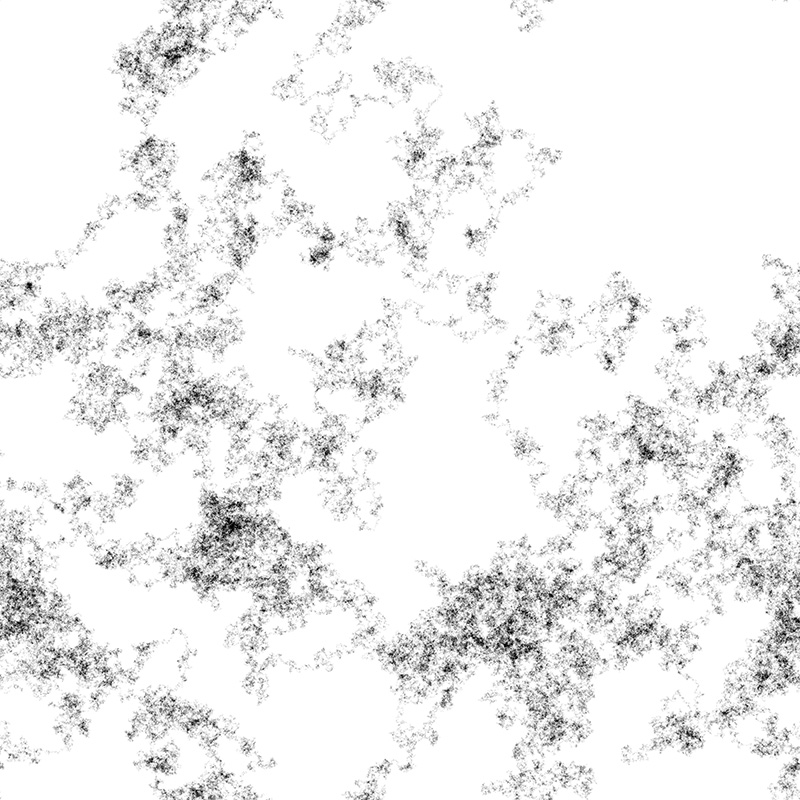
\includegraphics[width=0.50\linewidth]{figures/walk100.jpg}
  \caption{A 2-dimensional random walk of 100 iterations by Paul Bourke.}
  \label{fig:100-iteration random walk}
\end{figure}

\vspace*{\fill}

\doublespace


\onehalfspacing

% include each chapter...
\pagenumbering{arabic}
\singlespace
\begin{savequote}[75mm] %was 85
The artist-conceptor will have to be knowledgeable and inventive in such varied domains as mathematics, logic, physics, chemistry, biology, genetics, paleontology (for the evolution of forms), the human sciences and history; in short, a sort of universality, but one based upon, guided by and oriented toward forms and architectures. \\
\citeyearpar[Arts/Sciences: Alloys p.3]{Xenakis}
\qauthor{Iannis Xenakis} 
\end{savequote}

\chapter{Some Prerequisite Knowledge of Lilypond and Python}
\doublespace
\newthought{In my experience} composing scores with the help of computational systems, I have found that the Abjad Application Programming Interface\footnote{http://abjad.mbrsi.org/} for formalized score control provides the greatest power and flexibility. Abjad is significant because of the freedom with which it provides composers with the ability to manipulate their musical material and the ability to control not only the musical elements of a score, but also other graphic features as well. Every score that is created with Abjad is engraved by the Lilypond music notation engine.\footnote{http://lilypond.org/} Because of this interdependence, the composer should become familiar with Lilypond’s model of music notation as well as elements of Lilypond's syntax. Since Abjad is an API in the Python programming language,\footnote{https://www.python.org/} it is essential that the composer be familiar with writing Python code. In this chapter, some basic concerns about Lilypond and Python will be discussed, while information directly related to the Abjad API follows in chapter two.

	\section{Lilypond}

\pagestyle{fancy}
\renewcommand\headrulewidth{0pt}
\lhead{}\chead{}\rhead{\thepage}
\cfoot{}
    \subsection{Comparision with Other Software}
\newthought{Most modern composers} will be familiar with the plethora of options available for digital music engraving. The purpose of this paper is not to delve into the history of modern engraving practices, but it is important to note that, by far, the most popular engraving software available for the consumer market today are Finale\footnote{https://www.finalemusic.com/} and Sibelius,\footnote{https://www.avid.com/sibelius} with a few new robust programs like Dorico\footnote{https://www.dorico.com/} beginning to appear. These systems, packed with many features, are suitable for the majority of composers’ needs. They allow composers to be able to engrave pitches and rhythms in traditional Western notation and provide a number of formatting options that expand upon these traditions, allowing the user to create professional-quality documents, but it is not insignificant to note that many composers find the musical model of these programs to be overly restrictive upon musical creativity. As an example, with most of the common engraving software, users often must click through several menus to engrave a tuplet other than a triplet, especially if that tuplet does not contain successive rhythms of the same duration. Programs such as Dorico and the most recent versions of Finale have supplemented some of these issues through keyboard shortcuts\footnote{Most notation software also allows the user to define their own keyboard shortcuts.} and opened a clearer accessibility to the engraving of insected tuplets, but otherwise it is clear: these programs are tailored to a specific set of engraving requirements. This software is made for people engraving fairly traditional music like transcriptions, orchestrations, film scores, and so on, which do not typically make extensive use of this kind of notation.


While the programs are flexible and can be used for other means, I decided that what I require from a musical score is significantly restricted by the software. It becomes tedious to write music with many tuplets or other graphical oddities. While some composers have written their own engraving programs, like NoteAbility Pro,\footnote{http://debussy.music.ubc.ca/NoteAbility/} which can handle a number of contemporary techniques with ease, other composers have resorted to simply composing in graphic editors and drawing-oriented software, which brings the act of engraving much closer to the act of handwriting a piece; but even with these paradigm shifts, few notation engines show any friendliness to structural formalization. Finale and Sibelius have features that allow the user to program certain procedures,\footnote{I have mostly seen plugins related to layout spacing and harmonic analysis, but it is my understanding the there are more capabilities available.} but these are limited. Programs like Patch Work (and its kin Patch Work Graphic Language\footnote{http://www2.siba.fi/PWGL/}) and OpenMusic\footnote{http://repmus.ircam.fr/openmusic/home} were created in order to supplement this limitation. These programs allow the composer to manipulate data to represent musical elements which are then engraved within the program in the case of PWGL. In the case of OpenMusic, the elements are exported as MusicXML,\footnote{https://www.musicxml.com/} to be engraved by another software; but the complex MusicXML files produced by these programs are not always stable and often produce fallacious results or completely fail to convert.\footnote{Incidentally, my first serious attempt to learn Abjad stems exactly from the fact that neither Finale 2012 nor Dorico 1 could convert MusicXML files I had created in OpenMusic 6.12. OMLily was the salvation of this music, but engraving features of the score other than pitch and rhythm proved tedious.} The combination of Abjad and Lilypond surmounts many of these concerns. Abjad simply writes text files of Lilypond code, which removes the concern of file transfer errors, and Lilypond represents each element of a score, music, text, or graphic, in a syntax that is simple and consistent across a number of engraving complexities allowing the composer to engrave almost anything as part of the score.\footnote{This is possible because Lilypond inherently has no GUI and writing text files is the intended user interaction with the program. It is also possible because Lilypond is open source. Abjad could potentially be reworked to engrave music with a different engine, but Lilypond was and still is the most feasible option.} 

\subsection{Lilypond's Model of Musical Rhythm}

Another important aspect of Lilypond is its modelling of rhythmic content. Lilypond makes a distinction, unlike other notation engines, between written and prolated durations. In programs like OpenMusic, a set of triplet eighth notes would be written as durations of \( \frac{1}{3} \), \( \frac{1}{3} \), \( \frac{1}{3} \),\footnote{Often, composers use OpenMusic's RTM syntax which is comprised of LISP-like nested lists like the following, which does not model rhythm in the way described in this paragraph: (1 (3 (2 (1 2 -1 1)) 3))} but in Lilypond they would be written as \( \frac{1}{8} \), \( \frac{1}{8} \), \( \frac{1}{8} \) prolated by a duration of \( \frac{3}{2} \). This means that traditional rhythmic notation like whole notes through sixty-fourth notes and beyond are written as usual, but are prolated by a surrounding tuplet bracket with a given duration. Abjad follows, as much as possible, the same conventions as Lilypond’s notational model.

\subsection{Context Concatenation}

Lilypond also has a feature referred to as ``Context Concatenation.'' A context in Lilypond can be thought of as a staff with various features and formats associated with it. When given a name, a context is able to be appended to another context with the same name, as long as the files share the same score structure.\footnote{i.e. instrumentation as well as other invisible contexts} This allows the composer to write various sections of a piece in isolation and to stitch them together into a final document as a secondary process. Users should note a similarity between Lilypond syntax and \LaTeX \:\footnote{https://www.latex-project.org/} syntax, both of which share conceptual similarities with HTML\footnote{https://www.w3.org/html/} code. The following is a simple example of Lilypond syntax containing an unusual tuplet:\footnote{Note that it should be clear from this example that it is no more difficult to engrave this unusual tuplet than a regular triplet of straight eighth notes.}

\singlespace
\begin{lstlisting}[language=, caption=Lilypond syntax]
\version "2.19.82"
\language "english"
\score {
    \new Staff
    {   \times 2/9{
            c'8
            cs'8
            d'4.
            ef'8
            \times 3/2 {
                e'8
                f'8    }
              }
        fs'8
        g'8
        af'4
        a'4  }
}
\end{lstlisting}
\doublespace

		\section{Python}

\newthought{In Python}, there are a number of data types. Some of the important data types to address when discussing Abjad are integers, floating-point decimals, booleans, variables, strings, lists, tuples, and dictionaries. Each of these data types have specific features and behave in characteristic ways. Both integers and floating-point decimals, often called floats, are numbers. Integers can be used to signify numeric value in whole numbers while floats offer a more refined gradation of values. Variables are names that are assigned to other values or processes. With variables, users are able to refer to elements throughout a file without rewriting the information many times by hand.
    \subsection{Lists}
        \subsubsection{Slicing}
An important process to comprehend when composing with Abjad is that of list manipulation.\footnote{In fact, most of the work composers do when using Abjad involves storing and manipulating data in lists and dictionaries. Most elements of the score end up in a list at some point.} There are many processes that can be performed on and with lists. The concept of slicing will be discussed first. Readers vaguely familiar with Python may recognize the format $[x:y]$ when referring to slicing a list. In Python, the programmer can refer to items within a list via their indices. The index is the location within a list where an item exists. These indices begin at zero. An example set of indices is $[0, 1, 2, 3, 4, 5 …]$,\footnote{It is also possible to use a negative index. The first element of a list is still index 0, but the final element of the list is -1.} but the Python slices $[x:y]$ do not refer to items, even though indices do refer to items. The indicators within a slice actually refer to the spaces between items. It is possible to test this principle as follows:\footnote{This explanation comes from an email sent by Trevor Ba\v{c}a to the Abjad mailing list.}
\singlespace
\begin{lstlisting}[language=Python, caption=Printing an item of a list through indexing]
>>> letters = ['a', 'b', 'c', 'd', 'e', 'f']
>>> print(letters[2])
\end{lstlisting}
\doublespace
Which results in:
\singlespace
\begin{lstlisting}[language=, caption=Printing an item of a list through indexing: RESULT]
c
\end{lstlisting}
\doublespace
but:
\singlespace
\begin{lstlisting}[language=Python, caption=Printing items of a list through slicing]
>>> letters = ['a', 'b', 'c', 'd', 'e', 'f']
>>> print(letters[0:2])
\end{lstlisting}
\doublespace
results in:
\singlespace
\begin{lstlisting}[language=, caption=Printing items of a list through slicing: RESULT]
a
b
\end{lstlisting}
\doublespace
The following example presents a logical pitfall:
\singlespace
\begin{lstlisting}[language=Python, caption=Inserting elements into a list through slicing]
>>> letters = ['a', 'b', 'c', 'd', 'e', 'f']
>>> letters[-1:1] = 'xyz'
>>> print(letters)
\end{lstlisting}
\doublespace
Which will result in:
\singlespace
\begin{lstlisting}[language=, caption=Inserting elements into a list through slicing: RESULT]
['a', 'b', 'c', 'd', 'e', 'x', 'y', 'z', 'f']
\end{lstlisting}
\doublespace
It is demonstrated here that, in fact, this slicing refers to the continuous space between -1 and 1. The direction proceeds from right to left because the slice was begun with a negative number.

\subsubsection{List Comprehensions}

Another of the many actions that are able to be performed on lists is that of list comprehension. List comprehensions allow the programmer to quickly create lists whose contents follow simple parameters. Consider the built-in Python function $range()$, which allows the user to increment integers up until the user-input point. If Python were asked to print each item within $range(5)$, then $0, 1, 2, 3,$ and $4$ would be written to the terminal. A list comprehension could be written as follows:
\singlespace
\begin{lstlisting}[language=Python, caption=Creating a list with a list comprehension]
>>> foo = [x for x in range(5)]
>>> print(foo)
\end{lstlisting}
\doublespace
Which will result in:
\singlespace
\begin{lstlisting}[language=, caption=Creating a list with a list comprehension: RESULT]
[0, 1, 2, 3, 4]
\end{lstlisting}
\doublespace
It is also possible to act upon the elements within this list:
\singlespace
\begin{lstlisting}[language=Python, caption=Acting upon elements in a list comprehension]
>>> bar = [x*3 for x in range(5)]
>>> print(bar)
\end{lstlisting}
\doublespace
Which will result in:
\singlespace
\begin{lstlisting}[language=, caption=Acting upon elements in a list comprehension: RESULT]
[0, 3, 6, 9, 12]
\end{lstlisting}
\doublespace
This process can be substituted by a ``for loop,'' which is useful for more complicated functions, but can be overly verbose for processes better handled by list comprehensions:
\singlespace
\begin{lstlisting}[language=Python, caption=Rewriting a list comprehension as a ``for loop'']
>>> increments = range(5)
>>> spam = []
>>> for x in increments:
...	    spam.append(x*3)
>>> print(spam)
\end{lstlisting}
\doublespace
In this example, the built-in function $append()$ is used. It is important to make a distinction between append() and extend(). This can be illustrated as follows:
\singlespace
\begin{lstlisting}[language=Python, caption=Appending elements to a list]
>>> list_1 = [0, 1, 2, 3]
>>> list_2 = [4, 5, 6, 7]
>>> list_1.append(list_2)
>>> print(list_1)
\end{lstlisting}
\doublespace
Which results in:
\singlespace
\begin{lstlisting}[language=, caption=Appending elements to a list: RESULT]
[0, 1, 2, 3, [4, 5, 6, 7]]
\end{lstlisting}
\doublespace
but:
\singlespace
\begin{lstlisting}[language=Python, caption=Extending a list with elements]
>>> list_1 = [0, 1, 2, 3]
>>> list_2 = [4, 5, 6, 7]
>>> list_1.extend(list_2)
>>> print(list_1)
\end{lstlisting}
\doublespace
results in:
\singlespace
\begin{lstlisting}[language=, caption=Extending a list with elements: RESULT]
[0, 1, 2, 3, 4, 5, 6, 7]
\end{lstlisting}
\doublespace

    \subsection{Dictionaries}

A dictionary is much like a list, but in the case of a dictionary, elements of the list are referred to by keys:

\singlespace
\begin{lstlisting}[language=Python, caption=Printing elements from a dictionary]
musician = {'name':'Greg', 'instrument':'cello', 'age':24}
print(musician['instrument'])
\end{lstlisting}
\doublespace

resulting in:

\singlespace
\begin{lstlisting}[language=, caption=Printing elements from a dictionary: RESULT]
cello
\end{lstlisting}
\doublespace

Is is not possible to refer to elements in the dictionary from the right side of the key. The following example produces an error:

\singlespace
\begin{lstlisting}[language=Python, caption=Printing elements from a dictionary: ERROR]
musician = {'name':'Greg', 'instrument':'cello', 'age':24}
print(musician['cello'])
\end{lstlisting}
\doublespace

To make this kind of cross-definition work, the user must add the keys in reverse as follows:

\singlespace
\begin{lstlisting}[language=Python, caption=Printing elements from a dictionary: CORRECTION]
musician = {'name':'Greg', 'instrument':'cello', 'age':24, 'Greg':'name', 'cello':'instrument', 24:'age'}
print(musician['cello'])
\end{lstlisting}
\doublespace

\subsubsection{Dictionary Comprehensions}

Dictionary comprehensions are also possible and follow the same structure as list comprehensions:

\singlespace
\begin{lstlisting}[language=Python, caption=Making a dictionary comprehension]
keys =['Name', 'Instrument', 'Age']
definitions = ['Greg', 'Cello', 24]
musician = {key:definition for key, definition in zip(keys, definitions)}
print(musician)
\end{lstlisting}
\doublespace

resulting in:

\singlespace
\begin{lstlisting}[language=, caption=Making a dictionary comprehension: RESULT]
{'Name': 'Greg', 'Instrument': 'Cello', 'Age': 24}
\end{lstlisting}
\doublespace

\subsection{Modelling Objects}

One of the most attractive features of Abjad is that the system allows for the formalization of structures to control the placement and distribution of dynamics, articulations, and in fact, every visual element of the score. This is because Abjad attempts to model music notation rather than musical phenomenology. It treats all elements in a musical score as an object. An object in programming has various attributes and potential modes of behavior. An example of object modelling can be seen in the creation of animals. A first step is to create a general template on which the animals are based.

\singlespace
\begin{lstlisting}[language=Python, caption=Creating an empty class in python]
>>> class Animal:
... 	def __init__(self):
\end{lstlisting}
\doublespace

Attributes can be added to the basic animal in the \_\_init\_\_ section.

\singlespace
\begin{lstlisting}[language=Python, caption=Adding attributes to classes]
>>> class Animal:
... 	def __init__(self, name, color, pattern):
\end{lstlisting}
\doublespace

In order to retrieve the information that is placed in these attributes, the user must add the following below the \_\_init\_\_ section:

\singlespace
\begin{lstlisting}[language=Python, caption=Defining attributes in classes]
>>> class Animal:
... 	def __init__(self, name, color, pattern):
...		self.name = name
...		self.color = color
...		self.pattern = pattern
\end{lstlisting}
\doublespace

Now that an Animal object has been created, the programmer can begin to create individual animal types. One could create many animal objects to represent the menagerie, but a possible intermediate step would be to create a sub-class of the Animal. For instance, one could create a cat based on the general animal by doing the following:

\singlespace
\begin{lstlisting}[language=Python, caption=Creating a subclass]
>>> class Cat(Animal):
\end{lstlisting}
\doublespace

This cat has all of the same attributes that the general animal has. It is also possible to write functions to be included only in a specific sub-class:

\singlespace
\begin{lstlisting}[language=Python, caption=Adding methods to a subclass]
>>> class Cat(Animal):
...	def speak(self):
...		print('Purr...')
\end{lstlisting}
\doublespace

Likewise, other animals can be created in the same fashion:

\singlespace
\begin{lstlisting}[language=Python, caption=Creating more subclasses]
>>> class Dog(Animal):
...	def speak(self):
...		print('Woof...')
>>> class Giraffe(Animal):
...	def speak(self):
...		print('...giraffe sounds?')
\end{lstlisting}
\doublespace

Once the programmer has created objects to model different types of animals, specific animals with names, colors, and coat patterns can be defined by creating an instance of the animal objects.

\singlespace
\begin{lstlisting}[language=Python, caption=Instantiating objects with attribute values]
>>> huckle = Cat('huckle', 'orange', 'tabby')
>>> ginger = Dog('ginger', 'tan', 'fluffy')
>>> spooks = Cat('spooks', 'grey', 'tabby')
>>> geoffrey = Giraffe('geoffrey', 'brown and yellow', 'spotted')
\end{lstlisting}
\doublespace

These object instances can be queried for certain information:

\singlespace
\begin{lstlisting}[language=Python, caption=Interacting with objects]
>>> print('Huckle is ' + huckle.color)
>>> print('Spooks is a ' + spooks.pattern)
>>> print('The dog's name is ' + ginger.name)
>>> print('Geoffrey is ' + geoffrey.color)
>>> huckle.speak()
>>> spooks.speak()
>>> ginger.speak()
>>> geoffrey.speak()
\end{lstlisting}
\doublespace

Which results in the following output at the terminal:

\singlespace
\begin{lstlisting}[language=, caption=Interacting with objects: RESULT]
Huckle is orange
Spooks is a tabby
The dog's name is ginger
Geoffrey is brown and yellow
Purr...
Purr...
Woof!
...giraffe sounds?
\end{lstlisting}
\doublespace

Working with Python quickly becomes very complex, depending on the needs of the programmer, but much can be accomplished with an understanding of Python's data types, lists, dictionaries, and object modelling. In the following chapter, concepts in Lilypond and Python pertaining specifically to Abjad will be introduced in the context of my own use of the software for my compositional process.

\singlespace
\cleardoublepage
\phantomsection
\addcontentsline{toc}{chapter}{Blank Page}

\vspace*{\fill}
\begin{center}
This page is intentionally left blank.
\end{center}
\vspace*{\fill}
\begin{savequote}[75mm] 
One of the most significant areas of investigation in live instrumental music - that pertaining to the degree of approximation attained in any given realization of a particular type of musical text - offers itself most directly for transference into the computer studio, by reason of the obviously significant extent to which the concept of efficiency (in both human and computer terms) is (at least in real time) self-contradictory. \\
\citeyearpar[Composer-Computer-Active Form par.3]{Ferneyhough}
\qauthor{Brian Ferneyhough} 
\end{savequote}

\chapter{My Compositional Practice With Abjad, Lilypond, and Python}
\doublespace
	\section{Methodology}

\pagestyle{fancy}
\renewcommand\headrulewidth{0pt}
\lhead{}\chead{}\rhead{}
\cfoot{\vspace*{1.5\baselineskip}\thepage}

\newthought{In the preceding chapter}, I presented some of the strengths and potential weaknesses of Abjad and Lilypond when compared with similar programming paradigms, as well as some potential logical pitfalls when working with these programs. In my recent compositional practice, I have begun to amalgamate a workflow out of the ecosystem of Python, Abjad, and Lilypond, by learning from and embracing the idiosyncrasies of each. The use of these tools in tandem is advantageous for my work due to the flexibility of Lilypond's notational algorithm and Abjad’s clarification of Lilypond’s model of music notation through Python’s object-oriented nature, as well as Python’s vast logical and mathematical abilities. Not only are Abjad and Lilypond both full of diverse features, but due to their open source nature, the source code for each is accessible to the user for further modification. Occasionally, I have found the need to tweak Abjad's source code in order for it to perform functions that I desire, but more often than this, the composer will find the need to build tools to simplify the process of engraving.

In my work, I often desire a structural rigor, where rhythms, pitches, and orchestration, among other parameters are balanced together by a plan or logic that gives meaning to potential musical realities. A rigorous structure tends to fall apart when constructed by hand because humans are prone to err, while computers, conversely, do not make mistakes unless they are taught a false procedure. The computer does not have the ability to produce a logical fallacy unless the error is programmed into its underlying functionality. Because of this, working with the Python programming language allows for a consistency in formal rigor that might be otherwise unattainable by intuition or hand-written calculations and graphs. It also allows for the potential modeling of complex systems and algorithmic music, where human intuition is placed in a more subordinate role to formal design.

\pagestyle{fancy}
\renewcommand\headrulewidth{0pt}
\lhead{}\chead{}\rhead{\thepage}
\cfoot{}

Lilypond’s ability to draw lines and shapes, and its less restrictive model of notation than other software, allow the composer to have greater graphic freedom than other notation software. Another notable feature of Lilypond is its lack of a GUI,\footnote{Graphic User Interface} allowing the program more memory power when calculating spacing to avoid collisions, which results in greater visual clarity upon the first engraving of a piece. Also, since it allows the user to include functions in the Scheme programming language,\footnote{https://www.scheme.com/} the user is able to affect other features like proportional spacing across an entire score instead of manually clicking and dragging note heads as one would do while using Finale or Sibelius. Lilypond has the ability to manage all visual aspects of a score and can also be used to export image files in the $pdf$ and $png$ formats, along with $midi$ files. Finally, a great feature of Lilypond is its context concatenation ability. As mentioned in the previous chapter, this allows multiple, separate Lilypond files to be combined with one another to stitch together separate segments of a full composition into one document.


An advantage to the Abjad composition paradigm is its ability to manage polyphony. Other programming paradigms like PWGL or OM are a little more restrictive in this regard. Often, in PWGL and OM, using a procedure in one instrument as well as the next requires the user to instantiate a function multiple times and to alter the settings of the function in order for the music to seem continuous.\footnote{This issue would be solved with generators, but functions in OpenMusic don't naturally behave in this way. Admittedly, I do not know LISP very well and never wrote my own LISP functions in OM.} This duplication of processes that were carried out in other voices clutters up the workspace with redundant information. In Abjad, the two concepts of copying and continuing are very distinct,\footnote{This distinction, as mentioned earlier, comes from whether or not the programmer retrieves data from a generator or another reservoir.} allowing the composer to specifically use either technique as needed. Since Abjad is an API,\footnote{Application Programming Interface} in Python, it becomes very easy to cross-reference the same material-generating functions across different voices and at different points in time within the score. This comes from the fact that the music composed with Abjad is written as a text file, allowing composers to create and manipulate any object or function they choose; whereas programs like PWGL and OM are slightly restricted by their GUI. Though there are ways for composers to write their own functions in these programs, they are more difficult to manipulate and it is not entirely obvious to a beginner that it is even possible to do so. Because Abjad has no GUI, it inherently invites the composer to write the source code as part of the act of composition.


Though one could theoretically compose an entire score and only compile the Python file once the score is finalized, Abjad allows for an iterative workflow of composing, compiling, critiquing, and correcting in a cycle that lasts until the composer is satisfied with the composition. The speed of modern computation as opposed to hand written calculation and engraving makes this workflow reasonable. 


In Abjad, elements of a score are modeled as Python objects. Some objects, like a note or a rest for instance, have a duration attribute, but a note has an attribute that a rest does not: pitch. All elements of the score are objects with properties and attributes, therefore the entire score is manipulable via Abjad and, by extension, various formal means. This is a feature that is not present in OM and is difficult to achieve in PWGL, as OM does not display articulations or dynamics within the score viewing windows and PWGL’s interface is difficult to read.\footnote{Although many composers have had success with PWGL, its user interface has always seemed too cluttered to me and I have not explored it as thoroughly as I have OpenMusic.} This is, in part, because these programs have different foci and goals. OM is typically used like a calculator for composers to generate options for materials with which to compose and PWGL, while able to export data to other notation engines, is equipped with its own ENP,\footnote{Expressive Notation Package} with which music is rendered. Both OM and PWGL are based on CLOS,\footnote{Common LISP Object System} but I believe that the legibility of Python scripts as well as the large number of Python programmers makes it a much better candidate for the user-end of the system allowing for easy transference of knowledge from one user to another. The objects of notational elements are capable of being manipulated, therefore they can be created, connected, and appended to one another throughout the composition process to create a score through composer-written procedures and functions as well as through built-in tools. In the end, the greatest strength of this ecosystem is its flexibility.

In this chapter, I will discuss the compositional advantages of working with these programs such as how to automate potentially tedious tasks, the benefits of an iterative compositional workflow, and the possibilities for composing with algorithms or models. I will also explain some of my own solutions to composing with Abjad, like my $MusicMaker$ and $AttachmentHandlers$ classes as well as times when I have edited the Abjad source code.

\subsection{The Usefulness of Abjad for me as a Composer}

In my recent music, it is typical for me to focus significantly on formal uniformity and continuous, alternating procedures. These procedures might be in relation to the rhythmic, harmonic, textural, or dynamic material. I have also become very interested in a pseudo-tablature style of notation that features these iterative, procedural factors. It became apparent to me that I could leverage the programming concepts of loops and functions to write music very quickly. With this methodology I have written various programs that organize and produce musical material based on my predetermined structures, allowing me to compose material and generate the product of these procedures quickly. In the course of working in this manner, I have begun to appreciate the necessity of externalizing various tools in order to clean up my composition files. These tools, as well as my general compositional templates, could also easily be used by other composers, but they are tailored explicitly to my own compositional needs. Not only do my tools written in Python help me stay consistent with my formal designs, they also allow me to compose music that is specifically organized to my own tendencies and logic, rather than copying another composer’s tools and workflow. Although I have benefited greatly from the programs I have written, they are a work in progress and may not necessarily have universal functionality.\footnote{All code examples in this paper are written in Python 3, Abjad 3.1, and Lilypond 2.19.82.}

\subsection{Automating Potentially Tedious Tasks}

\subsubsection{Creating Notes}

There are two options for creating and viewing notes with Abjad. One could open up the terminal, or command line, and activate a Python session in order to write the code or alternatively, it is possible to write code in a text file saved with the $.py$ suffix and call Python to compile it once the file is completed. The former method is better for quick testing of loops and materials, while the second method is much more sustainable for the process of composing a score, because it allows the programmer to save progress as well as multiple versions of the code along the way. Regardless of which method is chosen, the code is written in the same way. The first step is always to import the Abjad API into the python session or file so that all of Abjad’s tools and properties are available. There are several ways of doing this, but the key to clarity is to be consistent. Throughout this chapter I will use this format:

\singlespace
\begin{lstlisting}[language=Python, caption=Import statement format]
>>> import abjad
\end{lstlisting}
\doublespace

This tells Python to instantiate tools through the Abjad namespace. Doing this requires that all Abjad objects be prefixed with $abjad.$ followed by whatever object or tool is being used. Thus, a note object will look like this:

\singlespace
\begin{lstlisting}[language=Python, caption=Format for object instantiation]
>>> abjad.Note()
\end{lstlisting}
\doublespace

This note can be given a variable name with which the user is able to refer to the note throughout the file and $abjad.show()$ can be used to quickly produce a $pdf$ file of this note:

\singlespace
\begin{lstlisting}[language=Python, caption=Showing an $abjad.Note()$ object]
>>> import abjad
>>> note = abjad.Note()
>>> abjad.show(note)
\end{lstlisting}
\doublespace

This Abjad code will produce a Lilypond file containing the following text:

\singlespace
\begin{lstlisting}[language=, caption=Showing an instance of an $abjad.Note()$ object: RESULT]
\version "2.19.82"  %! LilyPondFile
\language "english" %! LilyPondFile

\header { %! LilyPondFile
    tagline = ##f
} %! LilyPondFile

\layout {}

\paper {}

\score { %! LilyPondFile
    {
        c'4
    }
} %! LilyPondFile
\end{lstlisting}
\doublespace

and will produce the image in a pdf file seen in figure \ref{fig:default_note}:

\singlespace
\begin{figure}[h]
  \includegraphics[width=0.25\linewidth]{figures/fig1.png}
  \caption{A default note.}
  \label{fig:default_note}
\end{figure}
\doublespace

Notice that the note object has various default values associated with it. The note is rendered with a pitch value of middle c and a duration value of one quarter note. Easily enough, these values are manipulable! Instead, the following could have been written:\footnote{http://abjad.mbrsi.org/appendices/pitch\_conventions.html}

\singlespace
\begin{lstlisting}[language=Python, caption=Altering default values in an instance $abjad.Note()$ object]
>>> import abjad
>>> note = abjad.Note(11, abjad.Duration(1, 8))
>>> abjad.show(note)
\end{lstlisting}
\doublespace

from which the image in figure \ref{fig:b_natural} and the following Lilypond code would be received:

\singlespace
\begin{lstlisting}[language=, caption=Altering default values in an instance $abjad.Note()$ object: RESULT]
\score { %! LilyPondFile
    {
        b'8
    }
} %! LilyPondFile
\end{lstlisting}
\doublespace

\singlespace
\begin{figure}[h]
  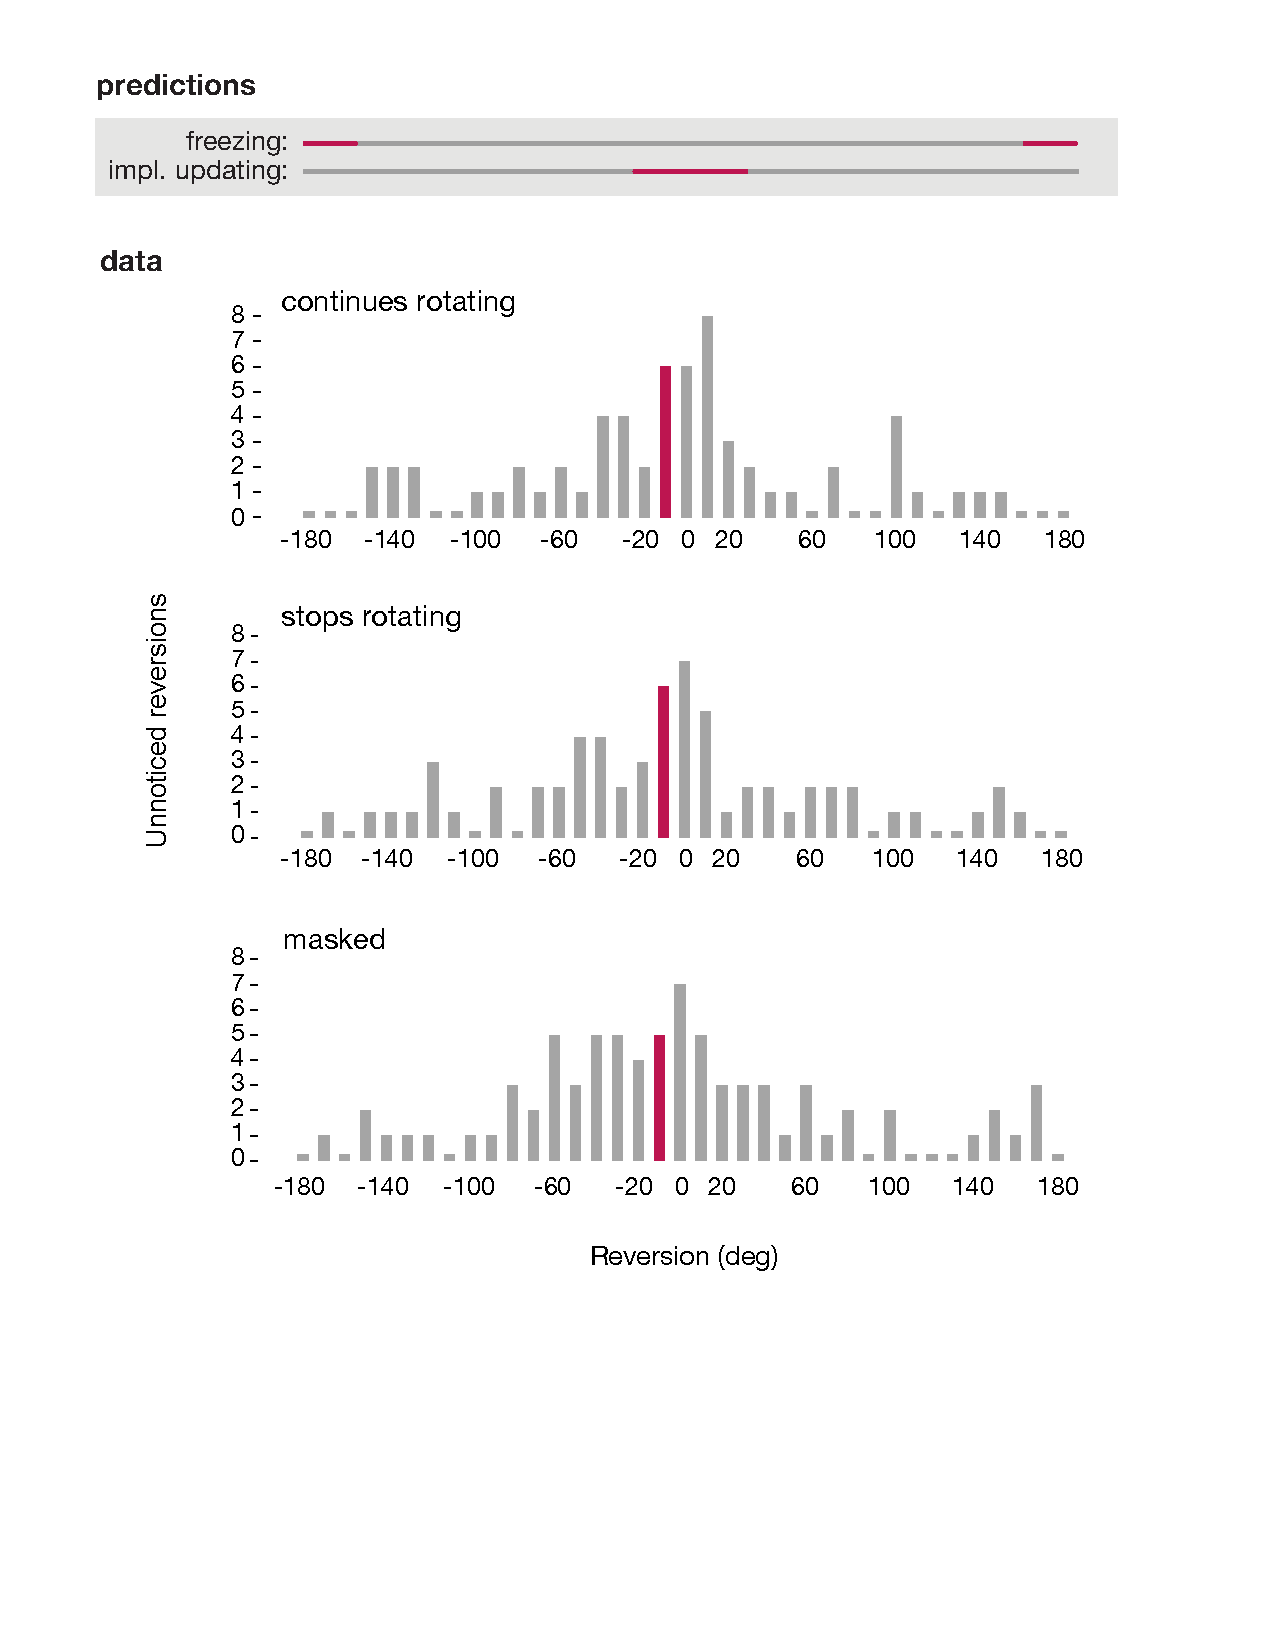
\includegraphics[width=0.21\linewidth]{figures/fig2.png}
  \caption{A note with the user-input duration value of (1, 8) and pitch value of 11.}
  \label{fig:b_natural}
\end{figure}
\doublespace

The following are a few strategies for making many notes in a row in order to create a piece. First, a staff and notes should be created. Then, the staff will be filled with notes and finally, the staff will be shown. Here is one way this can be done:

\singlespace
\begin{lstlisting}[language=Python, caption=Populating a staff with notes]
>>> import abjad
>>> note_1 = abjad.Note(0, abjad.Duration(1, 4))
>>> note_2 = abjad.Note(1, abjad.Duration(1, 4))
>>> note_3 = abjad.Note(2, abjad.Duration(1, 2))
>>> notes = [note_1, note_2, note_3]
>>> staff = abjad.Staff(notes)
>>> abjad.show(staff)
\end{lstlisting}
\doublespace

from which the user would receive figure \ref{fig:staff_with_pitches} and the following Lilypond code:

\singlespace
\begin{lstlisting}[language=, caption=Populating a staff with notes: RESULT]
\score { %! LilyPondFile
    \new Staff
    {
        c'4
        cs'4
        d'2
    }
} %! LilyPondFile
\end{lstlisting}
\doublespace

\singlespace
\begin{figure}[h]
  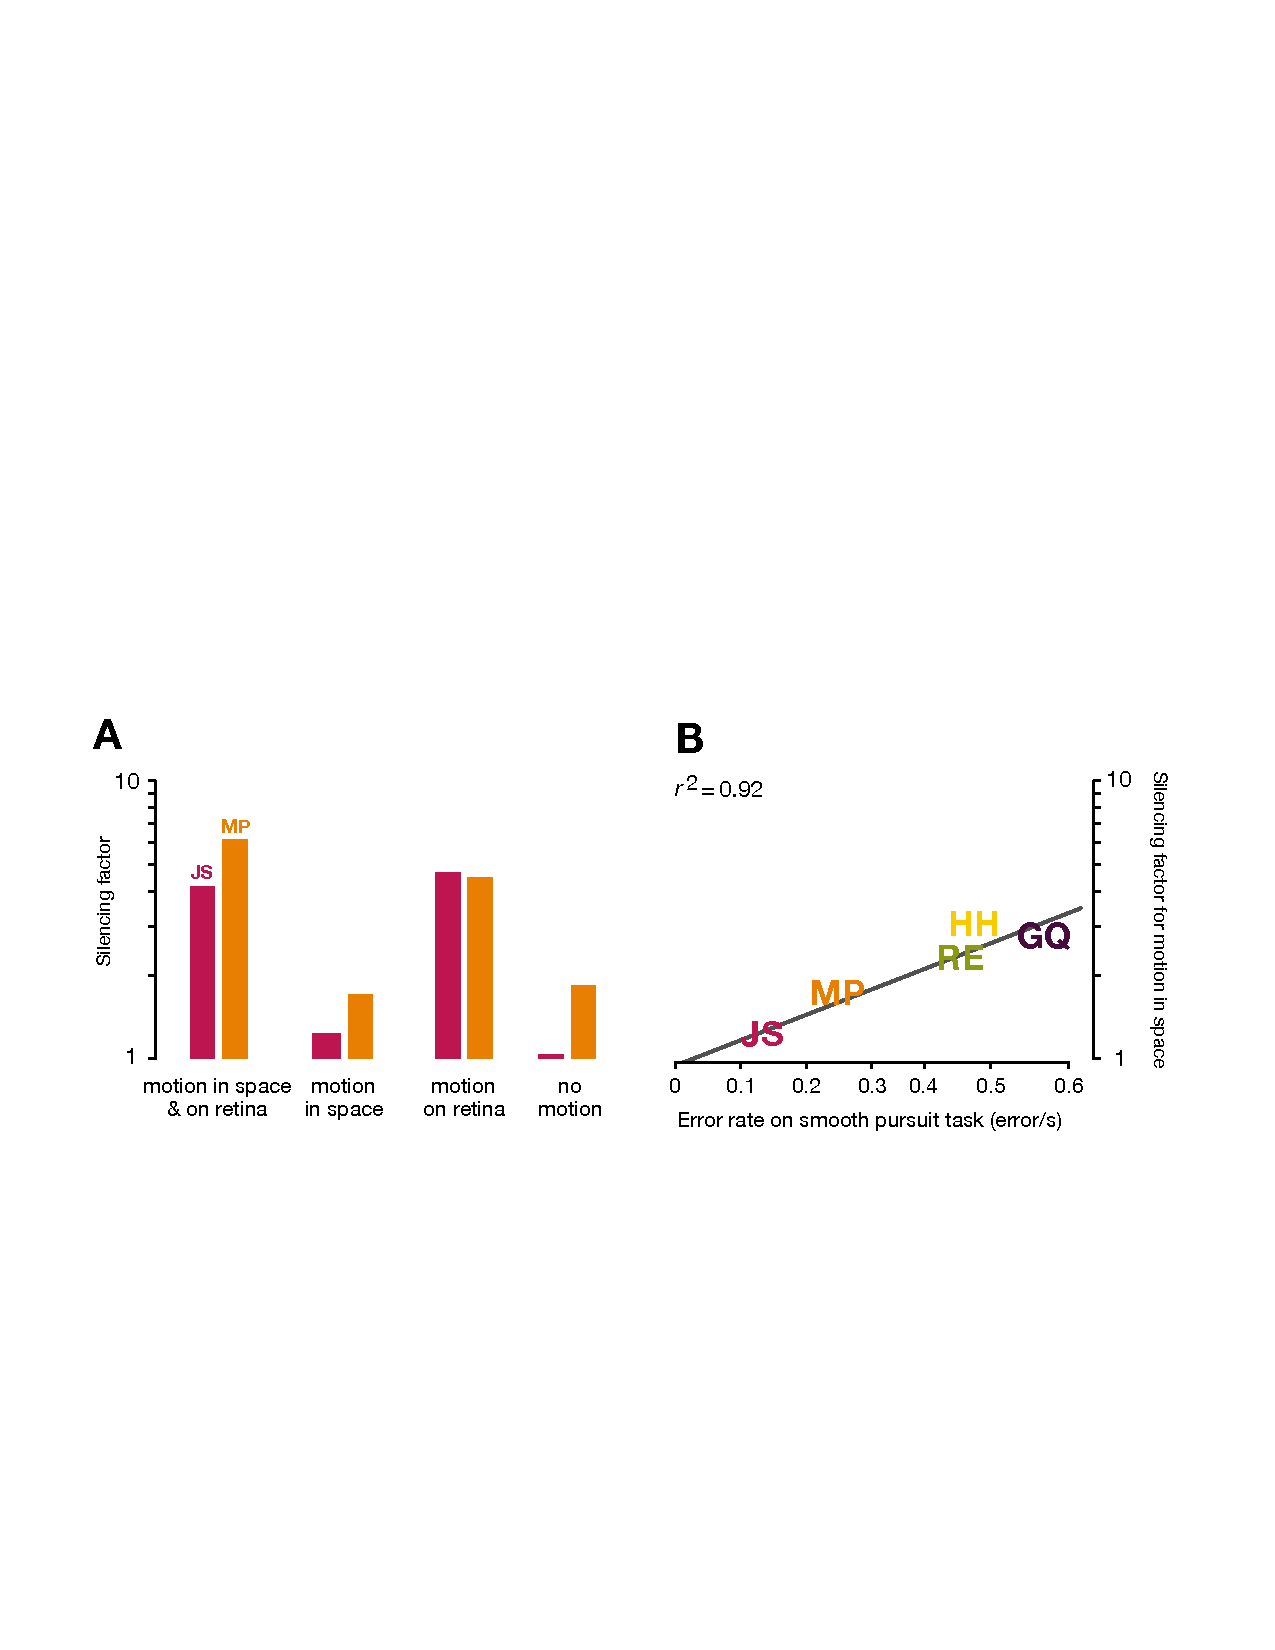
\includegraphics[width=0.36\linewidth]{figures/fig3.png}
  \caption{A staff with notes of varying pitch and duration.}
  \label{fig:staff_with_pitches}
\end{figure}
\doublespace

As one might begin to suspect, this process of note creation can get quite tedious. Here is one possible alternative approach to writing code with Abjad which is more economical for a longer piece:

\singlespace
\begin{lstlisting}[language=Python, caption=Faster note creation]
>>> import abjad
>>> numerators = [1, 1, 1, 1, 1, 1, 1, 3, 1, 1, 1, 1, ]
>>> denominators = [4, 4, 2, 8, 8, 4, 16, 16, 16, 16, 16, 16, ]
>>> durations = [abjad.Duration(y, z) for y, z in zip(numerators, denominators)]
>>> pitches = [0, 1, 2, 3, 4, 5, 6, 7, 8, 9, 10, 11]
>>> notes = [abjad.Note(x, y) for x, y in zip(pitches, durations)]
>>> note_staff = abjad.Staff(notes)
>>> abjad.show(note_staff)
\end{lstlisting}
\doublespace

Here, the use of $zip()$ can be seen as well as a list comprehension. With $zip()$ the programmer creates a list of numerators and denominators organized as tuples to represent fractions:

\singlespace
\begin{lstlisting}[language=, caption=Tuple zip: RESULT]
[(1, 4), (1, 4), (1, 2), (1, 8), (1, 8), (1, 4), (1, 16), (3, 16), (1, 16), (1, 16), (1, 16), (1, 16),]
\end{lstlisting}
\doublespace

and with this list comprehension a list of duration objects based on those fractions is returned:

\singlespace
\begin{lstlisting}[language=Python, caption=Duration list comprehension]
>>> [abjad.Duration(y, z) for y, z in zip(numerators, denominators)]
\end{lstlisting}
\doublespace

resulting in:	

\singlespace
\begin{lstlisting}[language=, caption=Duration list comprehension: RESULT]
[abjad.Duration((1, 4)), abjad.Duration((1, 4)), abjad.Duration((1, 2)), abjad.Duration((1, 8)), abjad.Duration((1, 8)), abjad.Duration((1, 4)), abjad.Duration((1, 16)), abjad.Duration((3, 16)), abjad.Duration((1, 16)), abjad.Duration((1, 16)), abjad.Duration((1, 16)), abjad.Duration((1, 16)),]
\end{lstlisting}
\doublespace

Again, two lists are zipped together, these being the list of pitches and the list of durations:

\singlespace
\begin{lstlisting}[language=, caption=Pitch and duration zip: RESULT]
[(0, abjad.Duration((1, 4))), (1, abjad.Duration((1, 4))), (2, abjad.Duration((1, 2))), (3, abjad.Duration((1, 8))), (4, abjad.Duration((1, 8))), (5, abjad.Duration((1, 4))), (6, abjad.Duration((1, 16))), (7, abjad.Duration((3, 16))), (8, abjad.Duration((1, 16))), (9, abjad.Duration((1, 16))), (10, abjad.Duration((1, 16))), (11, abjad.Duration((1, 16))),]
\end{lstlisting}
\doublespace

and a note object is created for every pitch and duration in this list with a list comprehension:

\singlespace
\begin{lstlisting}[language=, caption=Note object list comprehension: RESULT]
[abjad.Note(0, abjad.Duration((1, 4))), abjad.Note(1, abjad.Duration((1, 4))), abjad.Note(2, abjad.Duration((1, 2))), abjad.Note(3, abjad.Duration((1, 8))), abjad.Note(4, abjad.Duration((1, 8))), abjad.Note(5, abjad.Duration((1, 4))), abjad.Note(6, abjad.Duration((1, 16))), abjad.Note(7, abjad.Duration((3, 16))), abjad.Note(8, abjad.Duration((1, 16))), abjad.Note(9, abjad.Duration((1, 16))), abjad.Note(10, abjad.Duration((1, 16))), abjad.Note(11, abjad.Duration((1, 16))),]
\end{lstlisting}
\doublespace

this list of notes is placed inside of a staff and the staff is shown.

\singlespace
\begin{lstlisting}[language=Python, caption=Showing the staff]
>>> note_staff = abjad.Staff(notes)
>>> abjad.show(note_staff)
\end{lstlisting}
\doublespace

From this process, figure \ref{fig:staff_with_more_pitches} along with the following Lilypond output are produced:

\singlespace
\begin{lstlisting}[language=, caption=Showing the staff: RESULT]
\score { %! LilyPondFile
    \new Staff
    {
        c'4
        cs'4
        d'2
        ef'8
        e'8
        f'4
        fs'16
        g'8.
        af'16
        a'16
        bf'16
        b'16
    }
} %! LilyPondFile
\end{lstlisting}
\doublespace

\singlespace
\begin{figure}[h]
  \includegraphics[width=0.75\linewidth]{figures/fig13.png}
  \caption{A staff with many notes.}
  \label{fig:staff_with_more_pitches}
\end{figure}
\doublespace

If this kind of process is extrapolated, one can begin to create loops\footnote{a ``loop,'' or ``for loop'' is the name of a kind of function structure.} to handle tasks of every shape and size. Because this process can be arduous at times, Abjad is equipped with a number of tools out of the box to assist in processes like note creation such as $abjad.LeafMaker()$, $abjad.NoteMaker()$, $abjad.MeasureMaker()$, and $abjad.SegmentMaker()$. While these features are useful and are at the heart of many other tools like the Abjad-ext package $rmakers$, it is important to realize that it is not necessary to rely on these built-in functions to be able to write music with Abjad. 

\subsubsection{Dynamics, Articulations, and Hairpins}

Just like the creation of note objects, one can also simplify and formalize the attachment of dynamics:

\singlespace
\begin{lstlisting}[language=Python, caption=Attaching dynamics]
>>> import abjad
>>> dynamic_staff = abjad.Staff()
>>> dynamic_staff.extend(r"c'4 cs'4 d'2")
>>> piano = abjad.Dynamic('p')
>>> mezzo_forte = abjad.Dynamic('mf')
>>> forte = abjad.Dynamic('f')
>>> abjad.attach(piano, dynamic_staff[0])
>>> abjad.attach(mezzo_forte, dynamic_staff[1])
>>> abjad.attach(forte, dynamic_staff[2])
>>> abjad.show(dynamic_staff)
\end{lstlisting}
\doublespace

resulting in figure \ref{fig:dynamic_attachment_1} and the following Lilypond code:

\singlespace
\begin{lstlisting}[language=, caption=Attaching dynamics: RESULT]
\score { %! LilyPondFile
    \new Staff
    {
        c'4
        \p
        cs'4
        \mf
        d'2
        \f
    }
} %! LilyPondFile
\end{lstlisting}
\doublespace

\singlespace
\begin{figure}[h]
  \includegraphics[width=0.36\linewidth]{figures/fig5.png}
  \caption{Notes with dynamics.}
  \label{fig:dynamic_attachment_1}
\end{figure}
\doublespace

Simplifying this further by making use of a loop to attach the dynamics to each leaf\footnote{http://abjad.mbrsi.org/core\_concepts/lcsi.html} in the staff, dynamic objects can be created and attached at once:

\singlespace
\begin{lstlisting}[language=Python, caption=Attaching more dynamics]
>>> import abjad
>>> new_staff = abjad.Staff()
>>> new_staff.extend(r"c'4 cs'4 d'2 ef'8 e'8 f'4 fs'16 g'8. af'16 a'16 bf'16 b'16")
>>> dynamics = ['niente', 'pppp', 'ppp', 'pp', 'p', 'mp', 'mf', 'f', 'ff', 'fff', 'ffff', 'sfz', ]
>>> leaves = abjad.select(new_staff).leaves()
>>> for leaf, dynamic in zip(leaves, dynamics):
...     abjad.attach(abjad.Dynamic(dynamic), leaf)
>>> abjad.show(new_staff)
\end{lstlisting}
\doublespace

resulting in the Lilypond code and figure: \ref{fig:dynamic_attachment_1}:

\singlespace
\begin{lstlisting}[language=, caption=Attaching more dynamics: RESULT]
\score { %! LilyPondFile
    \new Staff
    {
        c'4
        _ #(make-dynamic-script (markup #:whiteout #:normal-text #:italic "niente"))
        cs'4
        \pppp
        d'2
        \ppp
        ef'8
        \pp
        e'8
        \p
        f'4
        \mp
        fs'16
        \mf
        g'8.
        \f
        af'16
        \ff
        a'16
        \fff
        bf'16
        \ffff
        b'16
        \sfz
    }
} %! LilyPondFile
\end{lstlisting}
\doublespace

\singlespace
\begin{figure}[h]
  \includegraphics[width=0.75\linewidth]{figures/fig14.png}
  \caption{More notes with dynamics.}
  \label{fig:dynamic_attachment_1}
\end{figure}
\doublespace

It can be seen that dynamics behave in the same way as other attachable objects. This is also true of articulations and hairpins. In the following example, articulations and hairpins are attached to leaves as well, featuring a possible way to imbue some behavioral qualities into the attachment of these elements.

\singlespace
\begin{lstlisting}[language=Python, caption=Attaching dynamics through an algorithm]
>>> import abjad
>>> music_staff = abjad.Staff()
>>> music_staff.extend(r"c'4 cs'4 d'2 r4 ds'2. e'8 f'8 fs'8 g'8 gs'8 r4. a'1")
>>> for run in abjad.select(music_staff).runs():
...     if len(run) > 3:
...         leaves = abjad.select(run).leaves()
...         abjad.attach(abjad.Dynamic('mf'), run[0])
...         for leaf in leaves:
...             abjad.attach(abjad.Articulation('tenuto'), leaf)
...     elif len(run) == 3:
...         abjad.attach(abjad.Dynamic('f'), run[0])
...         abjad.attach(abjad.StartHairpin('>'), run[0])
...         abjad.attach(abjad.Dynamic('mp'), run[-1])
...     elif len(run) == 1:
...         abjad.attach(abjad.Dynamic('ppp'), run[0])
>>> abjad.show(music_staff)
\end{lstlisting}
\doublespace

resulting in the Lilypond code and figure \ref{fig:dynamic_attachment_2}:

\singlespace
\begin{lstlisting}[language=, caption=Attaching dynamics through an algorithm: RESULT]
\score { %! LilyPondFile
    \new Staff
    {
        c'4
        \f
        \>
        cs'4
        d'2
        \mp
        r4
        e'2
        \mf
        - \tenuto
        f'8
        - \tenuto
        g'8
        - \tenuto
        a''8
        - \tenuto
        b''8
        - \tenuto
        c''8
        - \tenuto
        r4
        c''2.
        \ppp
    }
} %! LilyPondFile
\end{lstlisting}
\doublespace

\singlespace
\begin{figure}[h]
  \includegraphics[width=0.75\linewidth]{figures/fig6.png}
  \caption{Notes with algorithmic dynamics.}
  \label{fig:dynamic_attachment_2}
\end{figure}
\doublespace

This loop analyzes the length of each run in the staff and chooses what dynamics and articulations to attach based on the result. This is an extremely powerful method for attaching indicators throughout a score. Next, I will introduce a procedure to handle the $abjad.BowContactPoint()$ object, which produces a more complex Lilypond result and graphic.\footnote{For clean and legible notation, users will want to edit the Lilypond context in which this notation occurs to remove clefs and staff lines. An example of this can be seen in the following section on $Stylesheets$. In order to avoid confusion, examples featuring the $abjad.BowContactPoint$ too are engraved with the default staff context.}

\subsubsection{Using \textit{abjad.BowContactPoint()}}

The $abjad.BowContactPoint()$ object and an accompanying factory function, $abjad.bow\_contact\_spanner()$, are tools that are able to annotate a staff of notes with fractions intended to represent points along the length of a bow.\footnote{It makes no difference what pitches are in the staff because the note heads are removed by the tool.} Native in these tools is the ability to calculate whether one fraction is greater or lesser than its surrounding fractions and attach an ``up-bow'' or ``down-bow'' marking as needed. Because of this feature, I created a file in Abjad 2.21 which I called $abjad.StringContactSpanner$ which eliminated the bow markings in order for it to be used universally for any potential parameter. This file was adapted by Trevor Ba\v{c}a into Abjad 3.1’s $abjad.BowContactPoint()$ which features an optional keyword to include or exclude these bowings. Here is a possible way to use these tools:

\singlespace
\begin{lstlisting}[language=Python, caption=Bow tablature]
>>> import abjad
>>> bow_staff = abjad.Staff()
>>> bow_staff.extend(r"c'4 c'4 c'4 c'4")
>>> indicator_1 = abjad.BowContactPoint((3, 3))
>>> indicator_2 = abjad.BowContactPoint((2, 3))
>>> indicator_3 = abjad.BowContactPoint((1, 3))
>>> indicator_4 = abjad.BowContactPoint((0, 3))
>>> abjad.attach(indicator_1, bow_staff[0])
>>> abjad.attach(indicator_2, bow_staff[1])
>>> abjad.attach(indicator_3, bow_staff[2])
>>> abjad.attach(indicator_4, bow_staff[3])
>>> abjad.bow_contact_spanner(bow_staff, omit_bow_changes=True)
>>> abjad.show(bow_staff)
\end{lstlisting}
\doublespace

resulting in the Lilypond code:

\singlespace
\begin{lstlisting}[language=, caption=Bow tablature: RESULT]
\score { %! LilyPondFile
    \new Staff
    {
        \tweak Y-offset #2.0
        \tweak stencil #ly:text-interface::print
        \tweak text \markup {
            \center-align
                \vcenter
                    \fraction
                        1
                        1
            }
        c'4
        \glissando
        \tweak Y-offset #0.6666666666666666
        \tweak stencil #ly:text-interface::print
        \tweak text \markup {
            \center-align
                \vcenter
                    \fraction
                        2
                        3
            }
        c'4
        \glissando
        \tweak Y-offset #-0.6666666666666666
        \tweak stencil #ly:text-interface::print
        \tweak text \markup {
            \center-align
                \vcenter
                    \fraction
                        1
                        3
            }
        c'4
        \glissando
        \tweak Y-offset #-2.0
        \tweak stencil #ly:text-interface::print
        \tweak text \markup {
            \center-align
                \vcenter
                    \fraction
                        0
                        1
            }
        c'4
    }
} %! LilyPondFile
\end{lstlisting}
\doublespace

and figure \ref{fig:bow_contact_1}:

\singlespace
\begin{figure}[h]
  \includegraphics[width=0.25\linewidth]{figures/fig4.png}
  \caption{Bow tablature.}
  \label{fig:bow_contact_1}
\end{figure}
\doublespace

In the resultant Lilypond code are several, lengthy \textbackslash$tweak$ commands. Composing a score in Lilypond where an instrument has two staves, one of which is a bowing tablature that uses notation similar to what is produced by the $abjad.BowContactPoint()$ tool would be even more tedious to write than the note creation process above, making this tool quite useful for speeding up the engraving process. The following examples are a few alternative methods that achieve this kind of notation in a similar manner of reduction as in the note creation examples:

\singlespace
\begin{lstlisting}[language=Python, caption=Extended bow tablature]
>>> import abjad
>>> new_bow_staff = abjad.Staff()
>>> new_bow_staff.extend(r"c'4 c'4 c'2 c'8 c'8 c'4 c'16 c'8. c'16 c'16 c'16 c'16")
>>> indicator_1 = abjad.BowContactPoint((3, 3))
>>> indicator_2 = abjad.BowContactPoint((2, 3))
>>> indicator_3 = abjad.BowContactPoint((1, 3))
>>> indicator_4 = abjad.BowContactPoint((0, 3))
>>> indicator_5 = abjad.BowContactPoint((2, 3))
>>> indicator_6 = abjad.BowContactPoint((1, 3))
>>> indicator_7 = abjad.BowContactPoint((3, 3))
>>> indicator_8 = abjad.BowContactPoint((0, 3))
>>> indicator_9 = abjad.BowContactPoint((1, 3))
>>> indicator_10 = abjad.BowContactPoint((2, 3))
>>> indicator_11 = abjad.BowContactPoint((3, 3))
>>> indicator_12 = abjad.BowContactPoint((0, 3))
>>> indicators = [indicator_1, indicator_2, indicator_3, indicator_4, indicator_5,
... 			indicator_6, indicator_7, indicator_8, indicator_9, indicator_10,
...			indicator_11, indicator_12, ]
>>> leaves = abjad.select(new_bow_staff).leaves()
>>> for leaf, indicator in zip(leaves, indicators):
...     abjad.attach(indicator, leaf)
>>> abjad.bow_contact_spanner(new_bow_staff, omit_bow_changes=True)
\end{lstlisting}
\doublespace

resulting in the Lilypond code:

\singlespace
\begin{lstlisting}[language=, caption=Extended bow tablature: RESULT]
\score { %! LilyPondFile
    \new Staff
    {
        \tweak Y-offset #2.0
        \tweak stencil #ly:text-interface::print
        \tweak text \markup {
            \center-align
                \vcenter
                    \fraction
                        1
                        1
            }
        c'4
        \glissando
        \tweak Y-offset #0.6666666666666666
        \tweak stencil #ly:text-interface::print
        \tweak text \markup {
            \center-align
                \vcenter
                    \fraction
                        2
                        3
            }
        c'4
        \glissando
        \tweak Y-offset #-0.6666666666666666
        \tweak stencil #ly:text-interface::print
        \tweak text \markup {
            \center-align
                \vcenter
                    \fraction
                        1
                        3
            }
        c'2
        \glissando
        \tweak Y-offset #-2.0
        \tweak stencil #ly:text-interface::print
        \tweak text \markup {
            \center-align
                \vcenter
                    \fraction
                        0
                        1
            }
        c'8
        \glissando
        \tweak Y-offset #0.6666666666666666
        \tweak stencil #ly:text-interface::print
        \tweak text \markup {
            \center-align
                \vcenter
                    \fraction
                        2
                        3
            }
        c'8
        \glissando
        \tweak Y-offset #-0.6666666666666666
        \tweak stencil #ly:text-interface::print
        \tweak text \markup {
            \center-align
                \vcenter
                    \fraction
                        1
                        3
            }
        c'4
        \glissando
        \tweak Y-offset #2.0
        \tweak stencil #ly:text-interface::print
        \tweak text \markup {
            \center-align
                \vcenter
                    \fraction
                        1
                        1
            }
        c'16
        \glissando
        \tweak Y-offset #-2.0
        \tweak stencil #ly:text-interface::print
        \tweak text \markup {
            \center-align
                \vcenter
                    \fraction
                        0
                        1
            }
        c'8.
        \glissando
        \tweak Y-offset #-0.6666666666666666
        \tweak stencil #ly:text-interface::print
        \tweak text \markup {
            \center-align
                \vcenter
                    \fraction
                        1
                        3
            }
        c'16
        \glissando
        \tweak Y-offset #0.6666666666666666
        \tweak stencil #ly:text-interface::print
        \tweak text \markup {
            \center-align
                \vcenter
                    \fraction
                        2
                        3
            }
        c'16
        \glissando
        \tweak Y-offset #2.0
        \tweak stencil #ly:text-interface::print
        \tweak text \markup {
            \center-align
                \vcenter
                    \fraction
                        1
                        1
            }
        c'16
        \glissando
        \tweak Y-offset #-2.0
        \tweak stencil #ly:text-interface::print
        \tweak text \markup {
            \center-align
                \vcenter
                    \fraction
                        0
                        1
            }
        c'16
    }
} %! LilyPondFile
\end{lstlisting}
\doublespace

and figure \ref{fig:bow_contact_2}:

\singlespace
\begin{figure}[h]
  \includegraphics[width=0.75\linewidth]{figures/fig15.png}
  \caption{Extended bow tablature.}
  \label{fig:bow_contact_2}
\end{figure}
\doublespace

This example is very similar to the previous example, except for the fact that the process of attaching indicators to leaves has been streamlined. Here is another possibility:

\singlespace
\begin{lstlisting}[language=Python, caption=Very long bow tablature]
>>> import abjad
>>> new_bow_staff = abjad.Staff()
>>> new_bow_staff.extend(r"c'4 c'4 c'4 c'4 c'4 c'4 c'4 c'4 c'4 c'4 c'4 c'4")
>>> numerators = [3, 2, 1, 0, 1, 2, 3, 2, 1, 3, 0, 1, ]
>>> indicators = [(abjad.BowContactPoint((numerator, 3))) for numerator in numerators]
>>> leaves = abjad.select(new_bow_staff).leaves()
>>> for leaf, indicator in zip(leaves, indicators):
...     abjad.attach(indicator, leaf)
>>> abjad.bow_contact_spanner(new_bow_staff, omit_bow_changes=True)
>>> abjad.show(new_bow_staff)
\end{lstlisting}
\doublespace

resulting in the Lilypond code and figure \ref{fig:bow_contact_3}:

\singlespace
\begin{lstlisting}[language=, caption=Very long bow tablature: RESULT]
\score { %! LilyPondFile
    \new Staff
    {
        \tweak Y-offset #2.0
        \tweak stencil #ly:text-interface::print
        \tweak text \markup {
            \center-align
                \vcenter
                    \fraction
                        1
                        1
            }
        c'4
        \glissando
        \tweak Y-offset #0.6666666666666666
        \tweak stencil #ly:text-interface::print
        \tweak text \markup {
            \center-align
                \vcenter
                    \fraction
                        2
                        3
            }
        c'4
        \glissando
        \tweak Y-offset #-0.6666666666666666
        \tweak stencil #ly:text-interface::print
        \tweak text \markup {
            \center-align
                \vcenter
                    \fraction
                        1
                        3
            }
        c'4
        \glissando
        \tweak Y-offset #-2.0
        \tweak stencil #ly:text-interface::print
        \tweak text \markup {
            \center-align
                \vcenter
                    \fraction
                        0
                        1
            }
        c'4
        \glissando
        \tweak Y-offset #-0.6666666666666666
        \tweak stencil #ly:text-interface::print
        \tweak text \markup {
            \center-align
                \vcenter
                    \fraction
                        1
                        3
            }
        c'4
        \glissando
        \tweak Y-offset #0.6666666666666666
        \tweak stencil #ly:text-interface::print
        \tweak text \markup {
            \center-align
                \vcenter
                    \fraction
                        2
                        3
            }
        c'4
        \glissando
        \tweak Y-offset #2.0
        \tweak stencil #ly:text-interface::print
        \tweak text \markup {
            \center-align
                \vcenter
                    \fraction
                        1
                        1
            }
        c'4
        \glissando
        \tweak Y-offset #0.6666666666666666
        \tweak stencil #ly:text-interface::print
        \tweak text \markup {
            \center-align
                \vcenter
                    \fraction
                        2
                        3
            }
        c'4
        \glissando
        \tweak Y-offset #-0.6666666666666666
        \tweak stencil #ly:text-interface::print
        \tweak text \markup {
            \center-align
                \vcenter
                    \fraction
                        1
                        3
            }
        c'4
        \glissando
        \tweak Y-offset #2.0
        \tweak stencil #ly:text-interface::print
        \tweak text \markup {
            \center-align
                \vcenter
                    \fraction
                        1
                        1
            }
        c'4
        \glissando
        \tweak Y-offset #-2.0
        \tweak stencil #ly:text-interface::print
        \tweak text \markup {
            \center-align
                \vcenter
                    \fraction
                        0
                        1
            }
        c'4
        \glissando
        \tweak Y-offset #-0.6666666666666666
        \tweak stencil #ly:text-interface::print
        \tweak text \markup {
            \center-align
                \vcenter
                    \fraction
                        1
                        3
            }
        c'4
    }
} %! LilyPondFile
\end{lstlisting}
\doublespace

\singlespace
\begin{figure}[h]
  \includegraphics[width=0.65\linewidth]{figures/fig16.png}
  \caption{Very long bow tablature.}
  \label{fig:bow_contact_3}
\end{figure}
\doublespace

Here is a further simplification. In this code, the fractions in the indicators are summarized in a list comprehension. If this process is simplified even further it is possible to write code like this:

\singlespace
\begin{lstlisting}[language=Python, caption=Extremely long bow tablature]
>>> import abjad
>>> newer_bow_staff = abjad.Staff()
>>> newer_bow_staff.extend(r"c'8 c'8 c'8 c'8 c'8 c'8 c'8 c'8 c'8 c'8 c'8 c'8 c'8 c'8 c'8 ... 					c'8 c'8 c'8 c'8 c'8 c'8 c'8 c'8 c'8"
...					)
>>> leaves = abjad.select(newer_bow_staff).leaves()
>>> indicator_numerators = [3, 2, 1, 2, 1, 0, 3, 2, 0, 3, 1, 0, 0, 3, 2, 3, 2, 1, 1, 0, 3, ... 					2, 1, 0,
...					]
>>> for leaf, numerator in zip(leaves, indicator_numerators):
...     abjad.attach(abjad.BowContactPoint((numerator, 3)), leaf)
>>> abjad.bow_contact_spanner(newer_bow_staff, omit_bow_changes=True)
>>> abjad.show(newer_bow_staff)
\end{lstlisting}
\doublespace

resulting in the Lilypond code and figure \ref{fig:bow_contact_4}:

\singlespace
\begin{lstlisting}[language=, caption=Extremely long bow tablature: RESULT]
\score { %! LilyPondFile
    \new Staff
    {
        \tweak Y-offset #2.0
        \tweak stencil #ly:text-interface::print
        \tweak text \markup {
            \center-align
                \vcenter
                    \fraction
                        1
                        1
            }
        c'8
        \glissando
        \tweak Y-offset #0.6666666666666666
        \tweak stencil #ly:text-interface::print
        \tweak text \markup {
            \center-align
                \vcenter
                    \fraction
                        2
                        3
            }
        c'8
        \glissando
        \tweak Y-offset #-0.6666666666666666
        \tweak stencil #ly:text-interface::print
        \tweak text \markup {
            \center-align
                \vcenter
                    \fraction
                        1
                        3
            }
        c'8
        \glissando
        \tweak Y-offset #0.6666666666666666
        \tweak stencil #ly:text-interface::print
        \tweak text \markup {
            \center-align
                \vcenter
                    \fraction
                        2
                        3
            }
        c'8
        \glissando
        \tweak Y-offset #-0.6666666666666666
        \tweak stencil #ly:text-interface::print
        \tweak text \markup {
            \center-align
                \vcenter
                    \fraction
                        1
                        3
            }
        c'8
        \glissando
        \tweak Y-offset #-2.0
        \tweak stencil #ly:text-interface::print
        \tweak text \markup {
            \center-align
                \vcenter
                    \fraction
                        0
                        1
            }
        c'8
        \glissando
        \tweak Y-offset #2.0
        \tweak stencil #ly:text-interface::print
        \tweak text \markup {
            \center-align
                \vcenter
                    \fraction
                        1
                        1
            }
        c'8
        \glissando
        \tweak Y-offset #0.6666666666666666
        \tweak stencil #ly:text-interface::print
        \tweak text \markup {
            \center-align
                \vcenter
                    \fraction
                        2
                        3
            }
        c'8
        \glissando
        \tweak Y-offset #-2.0
        \tweak stencil #ly:text-interface::print
        \tweak text \markup {
            \center-align
                \vcenter
                    \fraction
                        0
                        1
            }
        c'8
        \glissando
        \tweak Y-offset #2.0
        \tweak stencil #ly:text-interface::print
        \tweak text \markup {
            \center-align
                \vcenter
                    \fraction
                        1
                        1
            }
        c'8
        \glissando
        \tweak Y-offset #-0.6666666666666666
        \tweak stencil #ly:text-interface::print
        \tweak text \markup {
            \center-align
                \vcenter
                    \fraction
                        1
                        3
            }
        c'8
        \glissando
        \tweak Y-offset #-2.0
        \tweak stencil #ly:text-interface::print
        \tweak text \markup {
            \center-align
                \vcenter
                    \fraction
                        0
                        1
            }
        c'8
        \glissando
        \tweak Y-offset #-2.0
        \tweak stencil #ly:text-interface::print
        \tweak text \markup {
            \center-align
                \vcenter
                    \fraction
                        0
                        1
            }
        c'8
        \glissando
        \tweak Y-offset #2.0
        \tweak stencil #ly:text-interface::print
        \tweak text \markup {
            \center-align
                \vcenter
                    \fraction
                        1
                        1
            }
        c'8
        \glissando
        \tweak Y-offset #0.6666666666666666
        \tweak stencil #ly:text-interface::print
        \tweak text \markup {
            \center-align
                \vcenter
                    \fraction
                        2
                        3
            }
        c'8
        \glissando
        \tweak Y-offset #2.0
        \tweak stencil #ly:text-interface::print
        \tweak text \markup {
            \center-align
                \vcenter
                    \fraction
                        1
                        1
            }
        c'8
        \glissando
        \tweak Y-offset #0.6666666666666666
        \tweak stencil #ly:text-interface::print
        \tweak text \markup {
            \center-align
                \vcenter
                    \fraction
                        2
                        3
            }
        c'8
        \glissando
        \tweak Y-offset #-0.6666666666666666
        \tweak stencil #ly:text-interface::print
        \tweak text \markup {
            \center-align
                \vcenter
                    \fraction
                        1
                        3
            }
        c'8
        \glissando
        \tweak Y-offset #-0.6666666666666666
        \tweak stencil #ly:text-interface::print
        \tweak text \markup {
            \center-align
                \vcenter
                    \fraction
                        1
                        3
            }
        c'8
        \glissando
        \tweak Y-offset #-2.0
        \tweak stencil #ly:text-interface::print
        \tweak text \markup {
            \center-align
                \vcenter
                    \fraction
                        0
                        1
            }
        c'8
        \glissando
        \tweak Y-offset #2.0
        \tweak stencil #ly:text-interface::print
        \tweak text \markup {
            \center-align
                \vcenter
                    \fraction
                        1
                        1
            }
        c'8
        \glissando
        \tweak Y-offset #0.6666666666666666
        \tweak stencil #ly:text-interface::print
        \tweak text \markup {
            \center-align
                \vcenter
                    \fraction
                        2
                        3
            }
        c'8
        \glissando
        \tweak Y-offset #-0.6666666666666666
        \tweak stencil #ly:text-interface::print
        \tweak text \markup {
            \center-align
                \vcenter
                    \fraction
                        1
                        3
            }
        c'8
        \glissando
        \tweak Y-offset #-2.0
        \tweak stencil #ly:text-interface::print
        \tweak text \markup {
            \center-align
                \vcenter
                    \fraction
                        0
                        1
            }
        c'8
    }
} %! LilyPondFile
\end{lstlisting}
\doublespace

\singlespace
\begin{figure}[h]
  \includegraphics[width=0.75\linewidth]{figures/fig17.png}
  \caption{Extremely long bow tablature.}
  \label{fig:bow_contact_4}
\end{figure}
\doublespace

This version of the code is comprised of the least number of lines. Both the fractions and the attachment processes are summarized in a loop that takes the fractions, puts them in an indicator and attaches those indicators each to a leaf of the staff. Notice that each version of the code results in the same kind of output and each option simplifies the process. Extensive use of $abjad.BowContactPoint()$ can be found in the compositions $Armilla$\footnote{https://github.com/josiah-wolf-oberholtzer/armilla} by Josiah Wolf Oberholtzer and $Cthar$ by Gregory Rowland Evans.

\subsubsection{Stylesheets}

An important concept when working with Lilypond is the idea of a stylesheet. Typically, the beginning of each Lilypond file will be full of information telling Lilypond how to format and render the music within the file. To make use of Lilypond’s context concatenation ability, it is best to externalize this information into a file called a stylesheet. An \textbackslash$include$ statement is used to let Lilypond know where to find this information. The stylesheet is written in Lilypond syntax and occasionally Scheme code and may feature information about horizontal spacing proportional to the duration of notes, vertical spacing in staff groups, the removal of time signatures within staves, and the creation of a new context for displaying those time signatures above the staff group. This is also where information about font, font size, paper size and orientation, and header information is stored. The following is the stylesheet that I wrote for my cello duo Cthar:

\singlespace
\begin{lstlisting}[language=, caption=Cthar stylesheet]
% 2018-07-17 19:54

\version "2.19.82"
\language "english"
#(set-default-paper-size "letterlandscape")
#(set-global-staff-size 10)
\include "ekmel.ily"
\ekmelicStyle evans

\header {
	tagline = ##f
	breakbefore = ##t
	title = \markup \override #'(
						font-name . "Didot"
						) \fontsize #15 \bold \center-column {
													"Cthar"
													}
	subtitle = \markup \override #'(
							font-name . "Didot"
							) \fontsize #4 \center-column {
													"for two cellos"
													}
	arranger = \markup \override #'(
							font-name . "Didot"
							) \fontsize #2.5 {
										"Gregory Rowland Evans"
										}
}

bowtab = {
   \override Staff.Clef.stencil = #ly:text-interface::print
   \override Staff.Clef.text = \markup { \general-align #Y #0.03
   \epsfile #Y #10 #"bow_position_tablature.eps"
   }
}

\layout {
    \accidentalStyle forget
    indent = #5
    ragged-right = ##t
	\context {
        \name TimeSignatureContext
        \type Engraver_group
        \numericTimeSignature
        \consists Axis_group_engraver
		\consists Bar_number_engraver
        \consists Time_signature_engraver
		\consists Mark_engraver
		\consists Metronome_mark_engraver
		\override BarNumber.Y-extent = #'(0 . 0)
		\override BarNumber.Y-offset = 0
		\override BarNumber.extra-offset = #'(-4 . 0)
		%\override BarNumber.font-name = "Didot"
		\override BarNumber.stencil = #(
							make-stencil-boxer 0.1 0.7 ly:text-interface::print
								)
		\override BarNumber.font-size = 1
		\override BarNumber.padding = 4
		\override MetronomeMark.X-extent = #'(0 . 0)
		\override MetronomeMark.Y-extent = #'(0 . 0)
		\override MetronomeMark.break-align-symbols = #'(left-edge)
		\override MetronomeMark.extra-offset = #'(0 . 4)
		\override MetronomeMark.font-size = 10
		\override RehearsalMark.stencil = #(
						make-stencil-circler 0.1 0.7 ly:text-interface::print
									)
		\override RehearsalMark.X-extent = #'(0 . 0)
		\override RehearsalMark.X-offset = 6
		\override RehearsalMark.Y-offset = -2.25
		\override RehearsalMark.break-align-symbols = #'(time-signature)
		\override RehearsalMark.break-visibility = #end-of-line-invisible
		\override RehearsalMark.font-name = "Didot"
		\override RehearsalMark.font-size = 8
		\override RehearsalMark.outside-staff-priority = 500
		\override RehearsalMark.self-alignment-X = #center
        \override TimeSignature.X-extent = #'(0 . 0)
        \override TimeSignature.X-offset = #ly:self-alignment-interface::x-aligned-on-self
        \override TimeSignature.Y-extent = #'(0 . 0)
		\override TimeSignature.Y-offset = 3
        \override TimeSignature.break-align-symbol = ##f
        \override TimeSignature.break-visibility = #end-of-line-invisible
        \override TimeSignature.font-size = #7
        \override TimeSignature.self-alignment-X = #center
        \override VerticalAxisGroup.default-staff-staff-spacing = #'(
												(basic-distance . 0) 
												(minimum-distance . 10) 
												(padding . 6) 
												(stretchability . 0)
												)
    }
    \context {
        \Score
        \remove Bar_number_engraver
		\remove Mark_engraver
        \accepts TimeSignatureContext
		\accepts LipStaff
		\override BarLine.bar-extent = #'(-2 . 2)
        \override Beam.breakable = ##t
		\override Beam.concaveness = #10000
		\override Glissando.breakable = ##t
		\override MetronomeMark.font-size = 5
        \override SpacingSpanner.strict-grace-spacing = ##t
        \override SpacingSpanner.strict-note-spacing = ##t
        \override SpacingSpanner.uniform-stretching = ##t
        \override StaffGrouper.staff-staff-spacing = #'(
										(basic-distance . 0) 
										(minimum-distance . 6) 
										(padding . 2)
										)
        \override TupletBracket.bracket-visibility = ##t
        \override TupletBracket.minimum-length = #3
        \override TupletBracket.padding = #2
        \override TupletBracket.springs-and-rods = #ly:spanner::set-spacing-rods
        \override TupletNumber.text = #tuplet-number::calc-fraction-text
		\override TextSpanner.Y-offset = 1
		proportionalNotationDuration = #(ly:make-moment 1 50)
        autoBeaming = ##f
        tupletFullLength = ##t
    }
	\context {
        \Voice
        \remove Forbid_line_break_engraver
    }
    \context {
        \Staff
        \remove Time_signature_engraver
    }
	\context {
        \Staff
        \name BowStaff
        \type Engraver_group
        \alias Staff
        \bowtab
        \override Beam.stencil = ##f
        \override Dots.stencil = ##f
        \override Flag.stencil = ##f
        \override Glissando.bound-details.left.padding = #0.5
        \override Glissando.bound-details.right.padding = #0.5
        \override Glissando.thickness = #2
        \override NoteHead.Y-offset = #-5
        \override NoteHead.extra-offset = #'(0.05 . 0)
		\override NoteHead.stencil = ##f
		\override Rest.transparent = ##t
        \override Script.staff-padding = #2
        \override StaffSymbol.transparent = ##t
        \override Stem.direction = #down
        \override Stem.stencil = ##f
        \override TimeSignature.stencil = ##f
		\override Tie.stencil = ##f
        \override TupletBracket.stencil = ##f
        \override TupletNumber.stencil = ##f
		%\RemoveEmptyStaves
    }

	\context {
        \Staff
        \name BeamStaff
        \type Engraver_group
        \alias Staff
        \override Beam.direction = #down
        \override Beam.positions = #'(5 . 5)
        \override Clef.stencil = ##f
        \override Dots.staff-position = #-2
        \override Flag.Y-offset = #2.93
        \override NoteHead.no-ledgers = ##t
        \override NoteHead.stencil = ##f
		\override Rest.transparent = ##t
        \override Script.staff-padding = #3
        \override StaffSymbol.transparent = ##t
        \override Stem.direction = #down
        \override Stem.length = #0.5
        \override Stem.stem-begin-position = #15.975
        \override TimeSignature.stencil = ##f
		\override Tie.stencil = ##f
        \override TupletBracket.positions = #'(3 . 3)
    }

    \context {
        \RhythmicStaff
        \remove Time_signature_engraver
    }
       \context {
        \StaffGroup
		\accepts BowStaff
		\accepts BeamStaff
    }
}

\paper {

	top-margin = 1.5\cm
	bottom-margin = 1.5\cm

	%top-margin = .90\in
	oddHeaderMarkup = \markup ""
	evenHeaderMarkup = \markup ""
	oddFooterMarkup = \markup \fill-line {
    ""
    \concat {
      "Cthar   ~"
	  \fontsize #2
	  \fromproperty #'page:page-number-string "~   Evans"
     }
    ""
  }
  evenFooterMarkup = \markup \fill-line {
    ""
	\concat { "Cthar   ~" \fontsize #2
	\fromproperty #'page:page-number-string "~   Evans"
    } ""
  }
}
\end{lstlisting}
\doublespace

In this score, I defined a few new contexts in order to manage the specific visual properties I desired for a staff indicating bow motion with the $abjad.BowContactPoint()$ tool. Aside from these properties, the composer is also able to edit graphic elements such as the width and spacing of beams, the thickness of stems, or the shape of flags. In this stylesheet, the clef symbol in the bowing staves is replaced with an $eps$ image of a bow to help indicate what the tablature represents.

These are just a few examples of ways in which Abjad and Lilypond allow for the simplification of processes that, by hand, could be extremely tedious over the course of a lengthy composition. The principles involved in these examples extend to every facet of both composing and engraving. Now that the power that Python can give composers has been described, next I will show how creating these loops and functions can have further ramifications in the process of composing.

\subsubsection{Composing with Models and Algorithms}

Composing with Abjad and Python allows the composer to work with models and algorithms. The following is an example where pitches are generated by a random walk which can be seen as a one-dimensional model of Brownian motion.\footnote{Brownian motion is a model used to describe the rapid and random motion of particles in a fluid.} Much of my recent music features a similar procedure as the following:

\singlespace
\begin{lstlisting}[language=Python, caption=Random walk]
>>> import abjad
>>> from random import seed
>>> from random import random
>>> seed(3)
>>> random_walk = []
>>> random_walk.append(-1 if random() < 0.5 else 1)
>>> for i in range(1, 64):
... 	movement = -1 if random() < 0.5 else 1
... 	value = random_walk[i-1] + movement
... 	random_walk.append(value)
>>> notes = [abjad.Note(x / 2.0, (1, 8)) for x in random_walk]
>>> staff = abjad.Staff(notes)
>>> abjad.show(staff)
\end{lstlisting}
\doublespace

In this code, the user must first create an empty list. Based on a string of randomly generated numbers, a new list of pitches is created, notated by numbers moving in a step of plus or minus 0.5 that are turned into note objects. They are next placed in a staff. It results in this Lilypond code and figure \ref{fig:random_walk}:

\singlespace
\begin{lstlisting}[language=, caption=Random walk: RESULT]
\score { %! LilyPondFile
    \new Staff
    {
        bqs8
        c'8
        bqs8
        c'8
        cqs'8
        c'8
        bqs8
        c'8
        bqs8
        b8
        bqs8
        b8
        bqs8
        b8
        bqs8
        b8
        bqs8
        c'8
        cqs'8
        cs'8
        dqf'8
        cs'8
        dqf'8
        d'8
        dqf'8
        cs'8
        dqf'8
        cs'8
        dqf'8
        d'8
        dqs'8
        ef'8
        dqs'8
        ef'8
        dqs'8
        ef'8
        eqf'8
        ef'8
        dqs'8
        d'8
        dqs'8
        d'8
        dqs'8
        d'8
        dqs'8
        d'8
        dqf'8
        d'8
        dqs'8
        ef'8
        eqf'8
        e'8
        eqs'8
        f'8
        fqs'8
        f'8
        fqs'8
        fs'8
        gqf'8
        g'8
        gqs'8
        g'8
        gqs'8
        af'8
    }
} %! LilyPondFile
\end{lstlisting}
\doublespace

\singlespace
\begin{figure}[h]
  \includegraphics[width=0.90\linewidth]{figures/fig7.png}
  \caption{A mapping of a random walk.}
  \label{fig:random_walk}
\end{figure}
\doublespace

It is also possible to model more traditional compositional algorithms.\footnote{Admittedly, mensuration canons do not present an extremely complex algorithm, but it meets my definition of algorithm.} This code is more complex than what we have seen before.\footnote{This code is adapted from code written by Jeffrey Trevi\~{n}o and presented as a part of the 2018 Abjad summer workshop at CCRMA\footnote{Center for Computer Research in Music and Acoustics} at Stanford University.} This code creates a three-voice canon based on the melody input by the user. The melody is transposed and the rhythms are scaled to a different tempo. Voices with phrases that end before the slowest voice completes its phrase are repeated until the bottom voice has finished. Because of how the rhythms are scaled, it is important to use $abjad.mutate().rewrite\_meter()$ to ensure that all rhythms remain in the appropriate measure:

\singlespace
\begin{lstlisting}[language=, caption=Mensuration canon]
>>> import abjad
>>> def generate_scaled_staff(scale_factor, staff):
...     staff_pitches = []
...     for logical_tie in abjad.iterate(staff).logical_ties():
...         first_leaf = logical_tie[0]
...         staff_pitches.append(first_leaf.written_pitch)
...     staff_durations = [
...	chain.written_duration*scale_factor for chain in abjad.iterate(staff).logical_ties()
...	]
...     scaled_staff = abjad.Staff()
...     maker = abjad.NoteMaker()
...     selections = maker(staff_pitches, staff_durations)
...     scaled_staff.extend(selections)
...     return scaled_staff

>>> def partition_value(value):
...     if x >= 16:
...         divisions, remainder = divmod(value, 8)
...         parts = [8] * divisions
...         if remainder:
...             parts.append(remainder)
...     return parts

>>> def process_maxima(durations):
...     output_durations = []
...     for duration in durations:
...         if duration[0] >= 16:
...             numerators = partition_value(duration[0])
...             duration = [(numerator, 1) for numerator in numerators]
...         output_durations.append(duration)

>>> def scale_and_chop_staff(voice_number, staff, time_signature):
...     scale_factor = 2 ** voice_number
...     scaled_staff = generate_scaled_staff(scale_factor, staff)
...     abjad.mutate(scaled_staff).transpose(voice_number * -7)
...     abjad.mutate(scaled_staff[:]).split([time_signature], cyclic=True)
...     return scaled_staff

>>> def duplicate_music(num_copies, staff):
...     out_staff = abjad.Staff()
...     for x in range(num_copies):
...         out_staff.extend(abjad.mutate(staff).copy())
...     return out_staff

>>> def make_scaled_staves(melody_staff, time_signature):
...     scaled_staves = []
...     for voice_number in range(3):
...       scaled_staff = scale_and_chop_staff(voice_number, melody_staff, time_signature)
...       scaled_staves.append(scaled_staff)
...     return scaled_staves

>>> def duplicate_score(scaled_staves):
...     score = abjad.Score()
...     for scaled_staff, duplicate_index in zip(scaled_staves, reversed(range(3))):
...         scale_factor = 2**duplicate_index
...         staff = duplicate_music(scale_factor, scaled_staff)
...         score.append(staff)
...     return score

>>> def format_score(score, key_signature, time_signature):
...     for staff in score:
...         key_sig = abjad.KeySignature(key_signature.tonic, key_signature.mode)
...         abjad.attach(key_sig, staff[0])
...         time_sig = abjad.TimeSignature(time_signature)
...         abjad.attach(time_sig, staff[0])
...     abjad.attach(abjad.Clef('varC'), score[1][0])
...     abjad.attach(abjad.Clef('bass'), score[2][0])

>>> def make_canon(melody_staff, key_signature, time_signature):
...     scaled_staves = make_scaled_staves(melody_staff, time_signature)
...     score = duplicate_score(scaled_staves)
...     format_score(score, key_signature, time_signature)
...     return score

>>> def rewrite_meter(score):
...     meter = abjad.Meter()
...     for staff in score:
...         for shard in abjad.mutate(staff[:]).split([abjad.Duration(4, 4)], cyclic=True):
...             abjad.mutate(shard).rewrite_meter(meter)

>>> melody_staff = abjad.Staff("c'4 cs'8 d' ds' e' f'4 fs' g' gs'8 a' b' c''")
>>> score = make_canon(
...	melody_staff, abjad.KeySignature('c', 'major'), abjad.TimeSignature((4,4))
...	)
>>> rewrite_meter(score)
>>> abjad.show(score)
\end{lstlisting}
\doublespace

resulting in the Lilypond code and figure \ref{fig:canon}:

\singlespace
\begin{lstlisting}[language=, caption=Mensuration canon: RESULT]
\score { %! LilyPondFile
    \new Score
    <<
        \new Staff
        {
            \key c \major
            \time 4/4
            c'4
            cs'8
            d'8
            ds'8
            e'8
            f'4
            fs'4
            g'4
            gs'8
            a'8
            b'8
            c''8
            c'4
            cs'8
            d'8
            ds'8
            e'8
            f'4
            fs'4
            g'4
            gs'8
            a'8
            b'8
            c''8
            c'4
            cs'8
            d'8
            ds'8
            e'8
            f'4
            fs'4
            g'4
            gs'8
            a'8
            b'8
            c''8
            c'4
            cs'8
            d'8
            ds'8
            e'8
            f'4
            fs'4
            g'4
            gs'8
            a'8
            b'8
            c''8
        }
        \new Staff
        {
            \key c \major
            \time 4/4
            \clef "varC"
            f2
            fs4
            g4
            gs4
            a4
            bf2
            b2
            c'2
            cs'4
            d'4
            e'4
            f'4
            f2
            fs4
            g4
            gs4
            a4
            bf2
            b2
            c'2
            cs'4
            d'4
            e'4
            f'4
        }
        \new Staff
        {
            \key c \major
            \time 4/4
            \clef "bass"
            bf,1
            b,2
            c2
            cs2
            d2
            ef1
            e1
            f1
            fs2
            g2
            a2
            bf2
        }
    >>
} %! LilyPondFile
\end{lstlisting}
\doublespace

\singlespace
\begin{figure}[h]
  \includegraphics[width=0.90\linewidth]{figures/fig8.png}
  \caption{A mensuration canon.}
  \label{fig:canon}
\end{figure}
\doublespace

Using Abjad and Python, composers are able to write music full of intricate relationships with precise formal consistency, but a comfortable formalism in score control is not necessarily algorithmic utopia. Though these logical procedures are available and entirely possible, they are optional. The process of composing with Abjad should not be misperceived as a purely algorithmic system for music composition. Certainly, formalizing elements in a score allows for a great amount of consistency and control, but composers have every ability to make decisions and sculpt the music at will if they so desire.\footnote{Composing with the workflow of Python, Abjad, and Lilypond does present some difficulty in composing idiomatically for instruments. Piano music, in particular, presents a great challenge, a challenge that I have yet to surmount. If one is not careful, it is possible to compose music completely unplayable by a human performer.} Abjad and Lilypond do not dictate what kind of music is able to be composed. It is still the duty of the composer to constrain their musical practices to those they consciously wish to deploy.

\subsection{The Need to Build Tools for a More Personalized Approach to Music-Making}

\subsubsection{Building Tools}

Why do I feel that it is important to write my own compositional tools? This is because each composer has a unique imagination and ideal. I feel greater satisfaction when I do not compose with the same methodology as another musician. I prefer a musical culture where each composer has a unique voice, because without it the beautiful diversity of new music would vanish. Abjad provides a framework for formalized score control but is not restrictive about the practices used to compose.\footnote{As I have previously written, even composing in notation programs such as Finale or Sibelius has restrictions and makes certain procedures difficult or impossible.} The fact that Abjad provides separate packages of tools for composition, as well as other functions, reveals that it is intended to be used by a variety of users with a variety of backgrounds. There are a handful of official extensions to Abjad under the title of abjad-ext.

\subsubsection{abjad-ext}

Abjad-ext consists of a number of packages that are not necessary for full functionality of the API. The packages include abjad-ext-tonality,\footnote{https://github.com/Abjad/abjad-ext-tonality} a tonal analysis extension, abjad-ext-book,\footnote{https://github.com/Abjad/abjad-ext-book} an extension for rendering Abjad code in \LaTeX, abjad-ext-ipython,\footnote{https://github.com/Abjad/abjad-ext-ipython} an extension for rendering Abjad code in IPython and Jupyter notebooks, abjad-ext-nauert,\footnote{https://github.com/Abjad/abjad-ext-nauert} an extension of quantization tools based on Paul Nauert’s Q-Grids, abjad-ext-cli,\footnote{https://github.com/Abjad/abjad-ext-cli} a Command Line Interface extension, and abjad-ext-rmakers,\footnote{https://github.com/Abjad/abjad-ext-rmakers} a rhythm maker tool extension. Each of these packages extend the functionality of Abjad, but I have only seriously used Trevor Ba\v{c}a’s rmakers package. These packages exist outside of the main Abjad source in order to emphasize their optionality.\footnote{The rmakers, previously called RhythmMakerTools, were once a part of the main Abjad source, but were externalized because their author felt they were more of a reflection of his own compositional practices than being a universal tool set.}

\subsubsection{rmakers}\footnote{make a subsubsubsection}

The rmakers consist of a set of tools for generating rhythmic material in certain characteristic ways. Contained in the rmakers package are a basic $RhythmMaker$ class, $AccelerandoRhythmMaker$, $EvenDivisionRhythmMaker$, $IncisedRhythmMaker$, $NoteRhythmMaker$, $TaleaRhythmMaker$, and $TupletRhythmMaker$. An extended description of these tools and their functionality can be found in Josiah Oberholtzer’s 2015 dissertation $A \: Computational \: Model \: of \: Music \: Composition$.\cite[pp. 118--128]{Oberholtzer} I am quite fond of these tools and, even though I intend to write my own rhythm-generating functions in the near future, they are the primary source of rhythmic composition in my recent music.

\subsection{Other Packages}

Along with the official abjad-ext packages are other packages by composers who make use of Abjad, including Consort,\footnote{https://github.com/josiah-wolf-oberholtzer/consort} a package written by Josiah Wolf Oberholtzer and described in detail in his dissertation, mtools\footnote{https://github.com/ivanalexandermoscotta/mtools} by Ivan Alexander Moscotta, and calliope\footnote{https://github.com/mirrorecho/calliope/tree/new-base} by Randall West. All of these packages present unique and innovative tools for music composition and have encouraged me to find my own way of composing with Abjad. As of the writing of this paper, I have only written one external tool set for composing, but they are used extensively in my scores, these are MusicMaker and the accompanying AttachmentHandler classes.

\subsection{MusicMaker}

MusicMaker is a python class of mine which is the result of my attempt to combine material consistency of many kinds. MusicMaker takes the input of an rmaker and an optional set of AttachmentHandler objects. This tool was written because, although the rmakers are capable of generating rhythmic material, they do not handle pitch in any way. One could compose the entire rhythmic framework of a piece and add pitches after the fact. I found myself using many different rmakers throughout the course of a piece and I found that I was working very hard to unify rhythmic gestures by giving them unique harmonic fields and dynamic trajectories. This process became quite difficult and required a trial-and-error process or a tedious amount of pre-compositional calculation by hand outside of the computer program. My solution was to create a tool that could handle many different rmakers, pitch fields, and attachment characteristics at once, leaving the composer to define distinct and alternating characters and processes with which to compose. When MusicMaker is given an rmaker and a list of pitches inside of the accompanying PitchHandler object, it automatically adds those pitches to the rhythms cyclically. When the list of pitches runs out, it repeats endlessly to ensure that there is always pitch material when the MusicMaker is called. Because MusicMaker generates music based on the rhythms and pitches that were input by the user each time that it is called within the python file, it allows the composer to instantiate multiple MusicMakers with unique rhythmic, harmonic, and dynamic qualities with other attachments. Much of my recent music is composed from alternating fragments of processes begun with MusicMaker. As I write more music, I find that there are more features that I wish to add to MusicMaker and the AttachmentHandler objects. As such, their code is still under revision. The following is the current source code for MusicMaker:

\singlespace
\begin{lstlisting}[language=Python, caption=MusicMaker source]
import abjad
from evans.AttachmentHandlers.GlissandoHandler import GlissandoHandler
from evans.AttachmentHandlers.NoteheadHandler import NoteheadHandler
from evans.AttachmentHandlers.PitchHandler import PitchHandler
from evans.AttachmentHandlers.ArticulationHandler import ArticulationHandler
from evans.AttachmentHandlers.DynamicHandler import DynamicHandler
from evans.AttachmentHandlers.TextSpanHandler import TextSpanHandler
from evans.AttachmentHandlers.ClefHandler import ClefHandler
from evans.AttachmentHandlers.SlurHandler import SlurHandler
from evans.AttachmentHandlers.TrillHandler import TrillHandler

class MusicMaker:
    def __init__(
        self,
        rmaker,
        glissando_handler=None,
        notehead_handler=None,
        pitch_handler=None,
        articulation_handler=None,
        dynamic_handler=None,
        text_span_handler=None,
        clef_handler=None,
        slur_handler=None,
        trill_handler=None,
        continuous=False,
        state=None,
    ):
        self.glissando_handler = glissando_handler
        self.notehead_handler = notehead_handler
        self.pitch_handler = pitch_handler
        self.articulation_handler = articulation_handler
        self.dynamic_handler = dynamic_handler
        self.text_span_handler = text_span_handler
        self.clef_handler = clef_handler
        self.slur_handler = slur_handler
        self.trill_handler = trill_handler
        self.continuous = continuous
        self.rmaker = rmaker
        self.state = self.rmaker.state
        self._count = 0

    def __call__(self, durations):
        return self._make_music(durations)

    def _make_basic_rhythm(self, durations):
        if self.continuous == True:
            state = self.state
            selections = self.rmaker(durations, previous_state=self.rmaker.state)
            self.state = self.rmaker.state
        else:
            selections = self.rmaker(durations, )
        return selections

    def _make_music(self, durations):
        selections = self._make_basic_rhythm(durations)
        if self.pitch_handler == None:
            start_command = abjad.LilyPondLiteral(
                r'\stopStaff \once \override Staff.StaffSymbol.line-count = #1 \startStaff',
                format_slot='before',
                )
            stop_command = abjad.LilyPondLiteral(
                r'\stopStaff \startStaff',
                format_slot='after',
                )
            literal = abjad.LilyPondLiteral(r'\once \override Staff.Clef.transparent = ##t', 'before')
            c_clef = abjad.LilyPondLiteral(r'\clef alto', 'before')
            abjad.attach(literal, selections[0][0])
            abjad.attach(c_clef, selections[0][0])
            abjad.attach(start_command, selections[0][0])
            abjad.attach(stop_command, selections[0][-1])
        if self.pitch_handler != None:
            selections = self.pitch_handler(selections)
            if self.clef_handler != None:
                selections = self.clef_handler(selections)
        if self.glissando_handler != None:
            selections = self.glissando_handler(selections)
        if self.notehead_handler != None:
            selections = self.notehead_handler(selections)
        if self.articulation_handler != None:
            selections = self.articulation_handler(selections)
        if self.dynamic_handler != None:
            selections = self.dynamic_handler(selections)
        if self.text_span_handler != None:
            selections = self.text_span_handler(selections)
        if self.slur_handler != None:
            selections = self.slur_handler(selections)
        if self.trill_handler != None:
            selections = self.trill_handler(selections)
        return selections
\end{lstlisting}
\doublespace

MusicMaker is made to be called with timespans\footnote{Timespans are also described in great detail in Josiah Oberholtzer's dissertation.\cite[pp. 78--118]{Oberholtzer}} and can be used as follows:

\singlespace
\begin{lstlisting}[language=Python, caption=Using MusicMaker with PitchHandler]
>>> import abjad
>>> import itertools
>>> import abjadext.rmakers
>>> from evans.AttachmentHandlers.MusicMaker import MusicMaker
>>> from evans.AttachmentHandlers.PitchHandler import PitchHandler

>>> time_signatures = [
...     abjad.TimeSignature(pair) for pair in [
...         (4, 4), (5, 4),
...     ]
... ]

>>> bounds = abjad.mathtools.cumulative_sums([_.duration for _ in time_signatures])

>>> rmaker_one = abjadext.rmakers.TaleaRhythmMaker(
...     talea=abjadext.rmakers.Talea(
...         counts=[1, 2, 3, 4],
...         denominator=16,
...         ),
...     beam_specifier=abjadext.rmakers.BeamSpecifier(
...         beam_divisions_together=True,
...         beam_rests=False,
...         ),
...     extra_counts_per_division=[0, 1,],
...     tuplet_specifier=abjadext.rmakers.TupletSpecifier(
...         trivialize=True,
...         extract_trivial=True,
...         rewrite_rest_filled=True,
...		 rewrite_sustained=True,
...         ),
...     )

>>> rmaker_two = abjadext.rmakers.EvenDivisionRhythmMaker(
...     denominators=[8, 16,],
...     extra_counts_per_division=[0,],
...     tuplet_specifier=abjadext.rmakers.TupletSpecifier(
...         trivialize=True,
...         extract_trivial=True,
...         rewrite_rest_filled=True,
...         ),
...     )

>>> musicmaker_one = MusicMaker(
...     rmaker=rmaker_one,
...     pitches=[0, 1, 2, 3, 4],
...     continuous=True,
... )
>>> musicmaker_two = MusicMaker(
...     rmaker=rmaker_two,
...     pitch_handler=PitchHandler(pitch_list=[4, 3, 2, 1, 0]),
...     continuous=True,
... )
>>> silence_maker = abjadext.rmakers.NoteRhythmMaker(
...     division_masks=[
...         abjadext.rmakers.SilenceMask(
...             pattern=abjad.index([0], 1),
...             ),
...         ],
...     )

>>> class MusicSpecifier:
...     def __init__(self, music_maker, voice_name):
...         self.music_maker = music_maker
...         self.voice_name = voice_name

>>> voice_1_timespan_list = abjad.TimespanList([
...     abjad.AnnotatedTimespan(
...         start_offset=start_offset,
...         stop_offset=stop_offset,
...         annotation=MusicSpecifier(
...             music_maker=music_maker,
...             voice_name='Voice 1',
...         ),
...     )
>>>     for start_offset, stop_offset, music_maker in [
...         [(0, 4), (2, 4), musicmaker_one],
...         [(2, 4), (3, 4), musicmaker_one],
...         [(3, 4), (4, 4), musicmaker_one],
...         [(6, 4), (8, 4), musicmaker_two],
...         [(8, 4), (9, 4), silence_maker],
...     ]
... ])

>>> all_timespan_lists = {
...     'Voice 1': voice_1_timespan_list,
... }

>>> global_timespan = abjad.Timespan(
...     start_offset=0,
...     stop_offset=max(_.stop_offset for _ in all_timespan_lists.values())
... )

>>> for voice_name, timespan_list in all_timespan_lists.items():
...     silences = abjad.TimespanList([global_timespan])
...     silences.extend(timespan_list)
...     silences.sort()
...     silences.compute_logical_xor()
...     for silence_timespan in silences:
...         timespan_list.append(
...             abjad.AnnotatedTimespan(
...                 start_offset=silence_timespan.start_offset,
...                 stop_offset=silence_timespan.stop_offset,
...                 annotation=MusicSpecifier(
...                     music_maker=None,
...                     voice_name=voice_name,
...                 ),
...             )
...         )
...     timespan_list.sort()

>>> for voice_name, timespan_list in all_timespan_lists.items():
...     shards = timespan_list.split_at_offsets(bounds)
...     split_timespan_list = abjad.TimespanList()
...     for shard in shards:
...         split_timespan_list.extend(shard)
...     split_timespan_list.sort()
...     all_timespan_lists[voice_name] = timespan_list

>>> score = abjad.Score([
...     abjad.Staff(lilypond_type='TimeSignatureContext', name='Global Context'),
...     abjad.Staff([abjad.Voice(name='Voice 1')],name='Staff 1', lilypond_type='Staff',),
...     ],
... )

>>> for time_signature in time_signatures:
...     skip = abjad.Skip(1, multiplier=(time_signature))
...     abjad.attach(time_signature, skip)
...     score['Global Context'].append(skip)

>>> def make_container(music_maker, durations):
...     selections = music_maker(durations)
...     container = abjad.Container([])
...     container.extend(selections)
...     return container

>>> def key_function(timespan):
...     return timespan.annotation.music_maker or silence_maker

>>> for voice_name, timespan_list in all_timespan_lists.items():
...     for music_maker, grouper in itertools.groupby(
...         timespan_list,
...         key=key_function,
...     ):
...         durations = [timespan.duration for timespan in grouper]
...         container = make_container(music_maker, durations)
...         voice = score[voice_name]
...         voice.append(container)

>>> for voice in abjad.iterate(score['Voice 1']).components(abjad.Voice):
...     for i , shard in enumerate(abjad.mutate(voice[:]).split(time_signatures)):
...         time_signature = time_signatures[i]
...         abjad.mutate(shard).rewrite_meter(time_signature)

>>> for voice in abjad.select(score).components(abjad.Voice):
...     for run in abjad.select(voice).runs():
...         specifier = abjadext.rmakers.BeamSpecifier(
...             beam_each_division=False,
...             )
...         specifier(run)
...     abjad.beam(voice[:], beam_lone_notes=False, beam_rests=False,)

>>> abjad.show(score)
\end{lstlisting}
\doublespace

With the assistance of a stylesheet for formatting, results in the following Lilypond code and figure \ref{fig:music_maker}:

\singlespace
\begin{lstlisting}[language=, caption=Using MusicMaker with PitchHandler: RESULT]
\score { %! LilyPondFile
    \new Score
    <<
        \context TimeSignatureContext = "Global Context"
        {
            \time 4/4
            s1 * 1
            \time 5/4
            s1 * 5/4
        }
        \context Staff = "Staff 1"
        {
            \context Voice = "Voice 1"
            {
                {
                    c'16
                    [
                    cs'16
                    ~
                    cs'16
                    d'16
                    ~
                    d'8
                    ef'8
                    ~
                    \times 4/5 {
                        ef'8
                        e'16
                        c'8
                    }
                    cs'8.
                    d'16
                    ]
                }
                {
                    r2
                }
                {
                    e'8
                    [
                    ef'8
                    d'8
                    cs'8
                    ]
                }
                {
                    r4
                }
            }
        }
    >>
} %! LilyPondFile
\end{lstlisting}
\doublespace

\singlespace
\begin{figure}[h]
  \includegraphics[width=0.75\linewidth]{figures/fig11.png}
  \caption{Notation from MusicMaker with two rmakers and PitchHandlers.}
  \label{fig:music_maker}
\end{figure}
\doublespace

\subsection{AttachmentHandlers}

Along with MusicMaker, I have written a number of AttachmentHandler tools to control many other musical features. The current list of functioning tools consists of ArticulationHandler, ClefHandler, DynamicHandler, GlissandoHandler, NoteheadHandler, PitchHandler, SlurHandler, and TrillHandler. As the names imply, each of these tools contain processes for the application of various graphical elements within a score. They can be called alongside MusicMaker to create far more complex musical gestures and to handle a number of engraving issues that would typically be surmounted by hand outside of the python file. The source code for these tools is included in the appendix to this paper. With the exception of TrillHandler, each of the AttachmentHandler tools is able to be used both within MusicMaker and elsewhere in a file. TrillHandler can be used as follows:

\singlespace
\begin{lstlisting}[language=Python, caption=Using TrillHandler]
>>> import abjad
>>> from TrillHandler import TrillHandler
>>> trill_handler = TrillHandler()
>>> staff = abjad.Staff(
... 		r'<a b>1 ~ <a b>4 \times 2/3 { a8 a8 <a b>8 } a4 a \times 2/3 { b8 a b }'
... 		)
>>> score = abjad.Score([staff])
>>> trill_handler(score)
>>> abjad.show(score)
\end{lstlisting}
\doublespace

It results in the following:

\singlespace
\begin{lstlisting}[language=, caption=Using TrillHandler: RESULT]
\version "2.19.82"  %! LilyPondFile
\language "english" %! LilyPondFile

\header { %! LilyPondFile
    tagline = ##f
} %! LilyPondFile

\layout {}

\paper {}

\score { %! LilyPondFile
    \new Score
    <<
        \new Staff
        {
            \pitchedTrill
            a1
            ~
            \startTrillSpan b
            a4
            \times 2/3 {
                a8
                \stopTrillSpan
                a8
                \pitchedTrill
                a8
                \startTrillSpan b
            }
            a4
            \stopTrillSpan
            a4
            \times 2/3 {
                b8
                a8
                b8
            }
        }
    >>
} %! LilyPondFile
\end{lstlisting}
\doublespace

and figure \ref{fig:trills}:

\singlespace
\begin{figure}[h]
  \includegraphics[width=0.50\linewidth]{figures/fig19.png}
  \caption{Trills.}
  \label{fig:trills}
\end{figure}
\doublespace

The following example is a few bars for four voices exhibiting the functionality of each of the AttachmentHandlers.

\singlespace
\begin{lstlisting}[language=Python, caption=Demonstration of AttachmentHandlers]
>>> import abjad
>>> import itertools
>>> import os
>>> import pathlib
>>> import time
>>> import abjadext.rmakers
>>> from MusicMaker import MusicMaker
>>> from ArticulationHandler import ArticulationHandler
>>> from ClefHandler import ClefHandler
>>> from DynamicHandler import DynamicHandler
>>> from GlissandoHandler import GlissandoHandler
>>> from NoteheadHandler import NoteheadHandler
>>> from PitchHandler import PitchHandler
>>> from SlurHandler import SlurHandler
>>> from TextSpanHandler import TextSpanHandler

>>> print('Interpreting file ...')

>>> time_signatures = [
...     abjad.TimeSignature(pair) for pair in [
...         (4, 4),
...     ]
... ]

>>> bounds = abjad.mathtools.cumulative_sums([_.duration for _ in time_signatures])

>>> rmaker = abjadext.rmakers.TaleaRhythmMaker(
...     talea=abjadext.rmakers.Talea(
...         counts=[2, 1, 5, 1, 3, 3, 1, 2, ],
...         denominator=16,
...         ),
...     beam_specifier=abjadext.rmakers.BeamSpecifier(
...         beam_divisions_together=True,
...         beam_rests=False,
...         ),
...     extra_counts_per_division=[0, 0, 1, 0, -1],
...     burnish_specifier=abjadext.rmakers.BurnishSpecifier(
...         left_classes=[abjad.Note, abjad.Rest],
...         left_counts=[1, 0, 1],
...         ),
...     tuplet_specifier=abjadext.rmakers.TupletSpecifier(
...         trivialize=True,
...         extract_trivial=True,
...         rewrite_rest_filled=True,
...         ),
...     )

>>> articulation_handler = ArticulationHandler(
...     articulation_list=['tenuto', 'staccato', 'portato', ],
...     continuous=True,
...     )

>>> clef_handler = ClefHandler(
...     clef='bass',
...     add_ottavas=True,
...     # ottava_shelf=5,
...     )

>>> dynamic_handler = DynamicHandler(
...     starting_dynamic='f',
...     hairpin='>',
...     ending_dynamic='p',
...     continuous=True,
...     )

>>> glissando_handler = GlissandoHandler(
...     line_style='dotted-line',
...     )

>>> notehead_handler = NoteheadHandler(
...     notehead_list=['cross', 'harmonic-mixed',
...                    'diamond', 'triangle', 'slash', 'default',  ],
...     continuous=True,
...     )

>>> pitch_handler = PitchHandler(
...     pitch_list=[0, 2, 1, [3, 10], 4, 8, [7, 9], 6],
...     continuous=True,
...     )

>>> slur_handler = SlurHandler(
...     slurs='runs',
...     )

>>> text_span_handler = TextSpanHandler(
...     position_list_one=['0/7', '5/7', '7/7', ],
...     position_list_two=['two', 'three', 'one', ],
...     position_list_three=['three', 'one', 'two', ],
...     start_style_one='solid-line-with-arrow',
...     start_style_two='dashed-line-with-arrow',
...     stop_style_one='solid-line-with-hook',
...     stop_style_two='dashed-line-with-hook',
...     stop_style_three='solid-line-with-hook',
...     apply_list_one_to='edges',
...     apply_list_two_to='ties',
...     apply_list_three_to='left_only',
...     continuous=True,
...     )

>>> music_maker = MusicMaker(
...     rmaker=rmaker,
...     articulation_handler=articulation_handler,
...     clef_handler=clef_handler,
...     dynamic_handler=dynamic_handler,
...     glissando_handler=glissando_handler,
...     notehead_handler=notehead_handler,
...     pitch_handler=pitch_handler,
...     slur_handler=slur_handler,
...     # text_span_handler=text_span_handler,
...     continuous=True,
... )

>>> silence_maker = abjadext.rmakers.NoteRhythmMaker(
...     division_masks=[
...         abjadext.rmakers.SilenceMask(
...             pattern=abjad.index([0], 1),
...             ),
...         ],
...     )

>>> class MusicSpecifier:

...     def __init__(self, rhythm_maker, voice_name):
...         self.rhythm_maker = rhythm_maker
...         self.voice_name = voice_name

>>> print('Collecting timespans and rmakers ...')

>>> voice_1_timespan_list = abjad.TimespanList([
...     abjad.AnnotatedTimespan(
...         start_offset=start_offset,
...         stop_offset=stop_offset,
...         annotation=MusicSpecifier(
...             rhythm_maker=rhythm_maker,
...             voice_name='Voice 1',
...         ),
...     )
...     for start_offset, stop_offset, rhythm_maker in [
...         [(0, 8), (4, 8), music_maker],
...         [(5, 8), (7, 8), music_maker],
...         [(7, 8), (8, 8), silence_maker],
...     ]
... ])

>>> voice_2_timespan_list = abjad.TimespanList([
...     abjad.AnnotatedTimespan(
...         start_offset=start_offset,
...         stop_offset=stop_offset,
...         annotation=MusicSpecifier(
...             rhythm_maker=rhythm_maker,
...             voice_name='Voice 2',
...         ),
...     )
...     for start_offset, stop_offset, rhythm_maker in [
...         [(0, 8), (4, 8), music_maker],
...         [(5, 8), (7, 8), music_maker],
...         [(7, 8), (8, 8), silence_maker],
...     ]
... ])

>>> voice_3_timespan_list = abjad.TimespanList([
...     abjad.AnnotatedTimespan(
...         start_offset=start_offset,
...         stop_offset=stop_offset,
...         annotation=MusicSpecifier(
...             rhythm_maker=rhythm_maker,
...             voice_name='Voice 3',
...         ),
...     )
...     for start_offset, stop_offset, rhythm_maker in [
...         [(0, 8), (4, 8), music_maker],
...         [(5, 8), (7, 8), music_maker],
...         [(7, 8), (8, 8), silence_maker],
...     ]
...])

>>> voice_4_timespan_list = abjad.TimespanList([
...     abjad.AnnotatedTimespan(
...         start_offset=start_offset,
...         stop_offset=stop_offset,
...         annotation=MusicSpecifier(
...             rhythm_maker=rhythm_maker,
...             voice_name='Voice 4',
...         ),
...     )
...     for start_offset, stop_offset, rhythm_maker in [
...         [(0, 8), (4, 8), music_maker],
...         [(5, 8), (7, 8), music_maker],
...         [(7, 8), (8, 8), silence_maker],
...     ]
...])

>>> all_timespan_lists = {
...     'Voice 1': voice_1_timespan_list,
...     'Voice 2': voice_2_timespan_list,
...     'Voice 3': voice_3_timespan_list,
...     'Voice 4': voice_4_timespan_list,
... }

>>> global_timespan = abjad.Timespan(
...     start_offset=0,
...     stop_offset=max(_.stop_offset for _ in all_timespan_lists.values())
... )

>>> for voice_name, timespan_list in all_timespan_lists.items():
...     silences = abjad.TimespanList([global_timespan])
...     silences.extend(timespan_list)
...     silences.sort()
...     silences.compute_logical_xor()
...     for silence_timespan in silences:
...         timespan_list.append(
...             abjad.AnnotatedTimespan(
...                 start_offset=silence_timespan.start_offset,
...                 stop_offset=silence_timespan.stop_offset,
...                 annotation=MusicSpecifier(
...                     rhythm_maker=None,
...                     voice_name=voice_name,
...                 ),
...             )
...         )
...     timespan_list.sort()

>>> for voice_name, timespan_list in all_timespan_lists.items():
...     shards = timespan_list.split_at_offsets(bounds)
...     split_timespan_list = abjad.TimespanList()
...     for shard in shards:
...         split_timespan_list.extend(shard)
...     split_timespan_list.sort()
...     all_timespan_lists[voice_name] = timespan_list

>>> score = abjad.Score([
...     abjad.Staff(lilypond_type='TimeSignatureContext', name='Global Context'),
...     abjad.StaffGroup(
...         [
abjad.Staff(
[abjad.Voice(name='Voice 1')],name='Staff 1', lilypond_type='Staff',
),
abjad.Staff(
[abjad.Voice(name='Voice 2')],name='Staff 2', lilypond_type='Staff',
),
abjad.Staff(
[abjad.Voice(name='Voice 3')],name='Staff 3', lilypond_type='Staff',
),
abjad.Staff(
[abjad.Voice(name='Voice 4')],name='Staff 4', lilypond_type='Staff',
),
...         ],
...         name='Staff Group',
...     )
... ])


>>> for time_signature in time_signatures:
...     skip = abjad.Skip(1, multiplier=(time_signature))
...     abjad.attach(time_signature, skip)
...     score['Global Context'].append(skip)

>>> print('Making containers ...')

>>> def make_container(rhythm_maker, durations):
...     selections = rhythm_maker(durations)
...     container = abjad.Container([])
...     container.extend(selections)
...     return container

>>> def key_function(timespan):
... 	return timespan.annotation.rhythm_maker or silence_maker

>>> for voice_name, timespan_list in all_timespan_lists.items():
...     for rhythm_maker, grouper in itertools.groupby(
...         timespan_list,
...         key=key_function,
...     ):
...         durations = [timespan.duration for timespan in grouper]
...         container = make_container(rhythm_maker, durations)
...         voice = score[voice_name]
...         voice.append(container)

>>> print('Beaming runs ...')
>>> for voice in abjad.select(score['Staff Group']).components(abjad.Voice):
...     for run in abjad.select(voice).runs():
...         specifier = abjadext.rmakers.BeamSpecifier(
...             beam_each_division=False,
...             )
...         specifier(run)
...     abjad.beam(voice[:], beam_lone_notes=False, beam_rests=False,)

>>> print('Stopping Hairpins and Text Spans...')

>>> for staff in abjad.iterate(score['Staff Group']).components(abjad.Staff):
...     for run in abjad.select(staff).runs():
...         last_leaf = run[-1]
...         next_leaf = abjad.inspect(last_leaf).leaf(1)
...         abjad.attach(abjad.StopHairpin(), next_leaf)

>>> print('Adding attachments ...')
>>> bar_line = abjad.BarLine('||')
>>> metro = abjad.MetronomeMark((1, 4), 108)
>>> markup = abjad.Markup(r'\bold { A }')
>>> mark = abjad.RehearsalMark(markup=markup)

>>> def cyc(lst):
...     count = 0
...     while True:
...         yield lst[count%len(lst)]
...         count += 1

>>> instruments = cyc([
...     abjad.Violin(),
...     abjad.Violin(),
...     abjad.Viola(),
...     abjad.Cello(),
...])

>>> clefs = cyc([
...     abjad.Clef('treble'),
...     abjad.Clef('treble'),
...     abjad.Clef('varC'),
...     abjad.Clef('bass'),
... ])

>>> abbreviations = cyc([
...     abjad.MarginMarkup(markup=abjad.Markup('vln. I'),),
...     abjad.MarginMarkup(markup=abjad.Markup('vln. II'),),
...     abjad.MarginMarkup(markup=abjad.Markup('vla.'),),
...     abjad.MarginMarkup(markup=abjad.Markup('vc.'),),
... ])

>>> names = cyc([
...     abjad.StartMarkup(markup=abjad.Markup('Violin I'),),
...     abjad.StartMarkup(markup=abjad.Markup('Violin II'),),
...     abjad.StartMarkup(markup=abjad.Markup('Viola'),),
...     abjad.StartMarkup(markup=abjad.Markup('Violoncello'),),
... ])

>>> for staff in abjad.iterate(score['Staff Group']).components(abjad.Staff):
...     leaf1 = abjad.select(staff).leaves()[0]
...     abjad.attach(next(instruments), leaf1)
...     abjad.attach(next(abbreviations), leaf1)
...     abjad.attach(next(names), leaf1)

>>> for staff in abjad.select(score['Staff Group']).components(abjad.Staff)[0]:
...     leaf1 = abjad.select(staff).leaves()[0]
...     last_leaf = abjad.select(staff).leaves()[-1]
...     abjad.attach(metro, leaf1)
...     abjad.attach(bar_line, last_leaf)

>>> for staff in abjad.iterate(score['Global Context']).components(abjad.Staff):
...     leaf1 = abjad.select(staff).leaves()[0]
...     abjad.attach(mark, leaf1)

>>> for staff in abjad.iterate(score['Staff Group']).components(abjad.Staff):
...     abjad.Instrument.transpose_from_sounding_pitch(staff)

>>> score_file = abjad.LilyPondFile.new(
...     score,
...     includes=['first_stylesheet.ily',
...			  '/Users/evansdsg2/abjad/docs/source/_stylesheets/abjad.ily'
...			],
...     )

>>> abjad.SegmentMaker.comment_measure_numbers(score)

>>> abjad.show(score_file)
\end{lstlisting}
\doublespace

It results in the following lilypond code:

\singlespace
\begin{lstlisting}[language=, caption=Demonstration of AttachmentHandlers: RESULT]
\version "2.19.82"  %! LilyPondFile
\language "english" %! LilyPondFile

\include "first_stylesheet.ily"                                      %! LilyPondFile
\include "/Users/evansdsg2/abjad/docs/source/_stylesheets/abjad.ily" %! LilyPondFile

\header { %! LilyPondFile
    tagline = ##f
} %! LilyPondFile

\layout {}

\paper {}

\score { %! LilyPondFile
    \new Score
    <<
        \context TimeSignatureContext = "Global Context"
        {
            % [Global Context measure 1] %! COMMENT_MEASURE_NUMBERS
            \time 4/4
            \mark \markup {
                \bold
                    {
                        A
                    }
                }
            s1 * 1
        }
        \context StaffGroup = "Staff Group"
        <<
            \context Staff = "Staff 1"
            \with
            {
                \consists Horizontal_bracket_engraver
            }
            {
                \context Voice = "Voice 1"
                {
                    {
                        % [Voice 1 measure 1] %! COMMENT_MEASURE_NUMBERS
                        \set Staff.shortInstrumentName =
                        \markup { "vln. I" }
                        \set Staff.instrumentName =
                        \markup { "Violin I" }
                        \tempo 4=108
                        \once \override Staff.NoteHead.style = #'cross
                        \clef "bass"
                        c'8
                        \f
                        - \tenuto
                        \>
                        - \tweak style #'dotted-line
                        \glissando
                        (
                        [
                        \once \override Staff.NoteHead.style = #'harmonic-mixed
                        d'16
                        - \staccato
                        - \tweak style #'dotted-line
                        \glissando
                        ]
                        \once \override Staff.NoteHead.style = #'diamond
                        cs'4
                        ~
                        - \tweak style #'dotted-line
                        \glissando
                        \once \override Staff.NoteHead.style = #'diamond
                        cs'16
                        \p
                        - \tweak stencil #constante-hairpin
                        \<
                        )
                    }
                    {
                        r8
                        \!
                    }
                    {
                        \once \override Staff.NoteHead.style = #'triangle
                        \clef "bass"
                        cs'16
                        \f
                        - \portato
                        \>
                        - \tweak style #'dotted-line
                        \glissando
                        (
                        [
                        \ottava 1
                        \once \override Staff.NoteHead.style = #'slash
                        <ef' bf'>8.
                        \p
                        - \tenuto
                        - \tweak stencil #constante-hairpin
                        \<
                        )
                        ]
                        \ottava 0
                    }
                    {
                        r8
                        \!
                        \bar "||"
                    }
                }
            }
            \context Staff = "Staff 2"
            \with
            {
                \consists Horizontal_bracket_engraver
            }
            {
                \context Voice = "Voice 2"
                {
                    {
                        \times 8/9 {
                            % [Voice 2 measure 1] %! COMMENT_MEASURE_NUMBERS
                            \set Staff.shortInstrumentName =
                            \markup { "vln. II" }
                            \set Staff.instrumentName =
                            \markup { "Violin II" }
                            \ottava 1
                            \once \override Staff.NoteHead.style = #'default
                            \clef "bass"
                            <ef' bf'>8.
                            \f
                            - \staccato
                            \>
                            - \tweak style #'dotted-line
                            \glissando
                            (
                            [
                            \ottava 0
                            \ottava 1
                            \once \override Staff.NoteHead.style = #'cross
                            e'16
                            - \portato
                            - \tweak style #'dotted-line
                            \glissando
                            \ottava 0
                            \ottava 1
                            \once \override Staff.NoteHead.style = #'harmonic-mixed
                            af'8
                            - \tenuto
                            - \tweak style #'dotted-line
                            \glissando
                            \ottava 0
                            \ottava 1
                            \ottava 1
                            \once \override Staff.NoteHead.style = #'diamond
                            <g' a'>8
                            - \staccato
                            - \tweak style #'dotted-line
                            \glissando
                            \ottava 0
                            \ottava 0
                            \ottava 1
                            \once \override Staff.NoteHead.style = #'triangle
                            fs'16
                            \p
                            - \portato
                            - \tweak stencil #constante-hairpin
                            \<
                            )
                            ]
                            \ottava 0
                        }
                    }
                    {
                        r8
                        \!
                    }
                    {
                        \ottava 1
                        \once \override Staff.NoteHead.style = #'slash
                        \clef "bass"
                        fs'4
                        \f
                        - \tenuto
                        - \tweak stencil #constante-hairpin
                        \<
                        )
                        (
                        \ottava 0
                    }
                    {
                        r8
                        \!
                    }
                }
            }
            \context Staff = "Staff 3"
            \with
            {
                \consists Horizontal_bracket_engraver
            }
            {
                \context Voice = "Voice 3"
                {
                    {
                        \tweak text #tuplet-number::calc-fraction-text
                        \times 8/7 {
                            % [Voice 3 measure 1] %! COMMENT_MEASURE_NUMBERS
                            \set Staff.shortInstrumentName =
                            \markup { vla. }
                            \set Staff.instrumentName =
                            \markup { Viola }
                            \ottava 1
                            \once \override Staff.NoteHead.style = #'default
                            \clef "bass"
                            fs'16
                            \f
                            - \staccato
                            \>
                            - \tweak style #'dotted-line
                            \glissando
                            (
                            [
                            \ottava 0
                            \once \override Staff.NoteHead.style = #'cross
                            c'16
                            - \portato
                            - \tweak style #'dotted-line
                            \glissando
                            \once \override Staff.NoteHead.style = #'harmonic-mixed
                            d'8.
                            - \tenuto
                            - \tweak style #'dotted-line
                            \glissando
                            \once \override Staff.NoteHead.style = #'diamond
                            cs'8
                            \p
                            - \staccato
                            - \tweak stencil #constante-hairpin
                            \<
                            )
                            ]
                        }
                    }
                    {
                        r8
                        \!
                    }
                    {
                        \once \override Staff.NoteHead.style = #'triangle
                        \clef "bass"
                        cs'16
                        \f
                        - \portato
                        \>
                        - \tweak style #'dotted-line
                        \glissando
                        (
                        [
                        \ottava 1
                        \once \override Staff.NoteHead.style = #'slash
                        <ef' bf'>16
                        - \tenuto
                        - \tweak style #'dotted-line
                        \glissando
                        \ottava 0
                        \ottava 1
                        \once \override Staff.NoteHead.style = #'default
                        e'8
                        \p
                        - \staccato
                        - \tweak stencil #constante-hairpin
                        \<
                        )
                        ]
                        \ottava 0
                    }
                    {
                        r8
                        \!
                    }
                }
            }
            \context Staff = "Staff 4"
            \with
            {
                \consists Horizontal_bracket_engraver
            }
            {
                \context Voice = "Voice 4"
                {
                    {
                        % [Voice 4 measure 1] %! COMMENT_MEASURE_NUMBERS
                        \set Staff.shortInstrumentName =
                        \markup { vc. }
                        \set Staff.instrumentName =
                        \markup { Violoncello }
                        \ottava 1
                        \once \override Staff.NoteHead.style = #'cross
                        \clef "bass"
                        e'8
                        \f
                        - \portato
                        \>
                        - \tweak style #'dotted-line
                        \glissando
                        (
                        [
                        \ottava 0
                        \ottava 1
                        \once \override Staff.NoteHead.style = #'harmonic-mixed
                        af'16
                        - \tenuto
                        - \tweak style #'dotted-line
                        \glissando
                        ]
                        \ottava 0
                        \ottava 1
                        \ottava 1
                        \once \override Staff.NoteHead.style = #'diamond
                        <g' a'>4
                        ~
                        - \tweak style #'dotted-line
                        \glissando
                        \once \override Staff.NoteHead.style = #'diamond
                        <g' a'>16
                        \p
                        - \tweak stencil #constante-hairpin
                        \<
                        )
                        \ottava 0
                        \ottava 0
                    }
                    {
                        r8
                        \!
                    }
                    {
                        \times 4/5 {
                            \ottava 1
                            \ottava 1
                            \once \override Staff.NoteHead.style = #'triangle
                            \clef "bass"
                            <g' a'>16
                            \f
                            - \staccato
                            \>
                            - \tweak style #'dotted-line
                            \glissando
                            (
                            [
                            \ottava 0
                            \ottava 0
                            \ottava 1
                            \once \override Staff.NoteHead.style = #'slash
                            fs'8.
                            - \portato
                            - \tweak style #'dotted-line
                            \glissando
                            \ottava 0
                            \once \override Staff.NoteHead.style = #'default
                            c'16
                            \p
                            - \tenuto
                            - \tweak stencil #constante-hairpin
                            \<
                            )
                            ]
                        }
                    }
                    {
                        r8
                        \!
                    }
                }
            }
        >>
    >>
} %! LilyPondFile
\end{lstlisting}
\doublespace

and figure \ref{fig:quartet}:

\singlespace
\begin{figure}[h]
  \includegraphics[width=0.75\linewidth]{figures/fig18.png}
  \caption{Four voice demonstration of AttachmentHandlers.}
  \label{fig:quartet}
\end{figure}
\doublespace

\section{Editing Source Code}

While I have written my own tools for composition with Abjad, I have also occasionally found it necessary to edit Abjad’s source code in order to include features that I desire, which is possible because Abjad is open source.

\subsection{Clef.py}

Recently I edited the $Clef.py$ file in the Abjad source. I did this in order to include Abjad representations of clefs that were present in the most recent update of Lilypond. The clefs in question were $varC$ and $tenorvarC$, both of which are alternative ``c'' clefs. I wanted to add these clefs for a logical reason as well as a personal reason. The first reason is that, as much as possible, Abjad should have a representation of all of Lilypond’s features. If a composer knows that Lilypond is capable of producing a certain graphic object,\footnote{These are often called grobs in Lilypond-lingo.} it can be very frustrating to find no way to use it in Abjad. The second reason is that these clefs more closely represent my own handwriting of c clefs than the traditional c clef.

\subsection{Articulation.py}

Just as with $Clef.py$ I also recently edited the $Articulation.py$ file. I did this at the same time and for the same reason as editing the clef file. I added Abjad representations of ``halfopen,'' which is a circle with a diagonal slash and ``snappizzicato,'' which is the common notation for a snap or ``Bartok'' pizzicato.

\subsection{Microtonal Expansion in Abjad 2.21}

In the summer of 2018, I undertook, with help from Ivan Moscotta, a much larger revision of Abjad’s source code. These edits were specifically centered around Abjad’s representation of pitch. At the time, the most recent version of Abjad was Abjad 2.21. Also during this summer, I attended the CCRMA Abjad workshop and I was able to discuss some of these changes with the primary maintainers of the system: Trevor Ba\v{c}a and Josiah Oberholtzer. We came to the conclusion that much of Abjad’s representation of microtones should be reassessed and should be open enough for composers to be able to define their own accidentals and scales. Because of this decision, the changes that I made to Abjad 2.21’s code are not available for users in the main branch of Abjad 3.1, but will hopefully be given new birth in a future release.\footnote{However, these changes are available in my greg/dev branch of Abjad.}

\subsubsection{Process}

I decided to undertake this major revision because I wanted to compose with microtones smaller than Lilypond’s and Abjad’s smallest interval, which is the quarter tone. In Lilypond’s font, Emmantaler, are two different kinds of quarter tones. Quarter tones written in Stein-Ellis notation and quarter tones written as traditional accidentals with an attached arrow either up or down to represent the microtonal alteration. I decided to use these arrow-based quarter tones to represent eighth tones.\footnote{This decision is informed, in part, by my familiarity with OpenMusic's accidentals.} In fact, there is a file buried deep within Lilypond called $Microtonal.ily$ that does just this. The file must be included at the header of the Lilypond file in order to make use of the user-defined microtones. I tried to find a way to do this and had a little success, although with great difficulty. I began to wonder if it was possible to extend this to further divisions of the octave. I began to edit the default font in Lilypond to be able to represent different kinds of accidentals as well as making some slight changes to the default accidentals for my own graphic preference, generally keeping to the Stein-Zimmerman notation for quarter tones\footnote{https://w3c.github.io/smufl/gitbook/tables/extended-stein-zimmermann-accidentals.html} and the Ferneyhough notation for all other microtonal alterations.\footnote{https://w3c.github.io/smufl/gitbook/tables/other-accidentals.html} This became cumbersome and inconsistent and I looked for an alternative. Fortuitously, I found the Ekmelily system.\footnote{http://www.ekmelic-music.org/en/extra/ekmelily.htm} This extension of Lilypond, written by Thomas Richter, does something similar to $Microtonal.ily$, but it also comes with an extensive font extension to allow for many kinds of microtonal representations and the ability to create user-defined scales with accidental grobs chosen by the user. This was my solution for graphically representing my new microtones. The following image in figure \ref{fig:scale} is a representation of my own user-defined scale:

\singlespace
\begin{figure}[h]
  \includegraphics[width=0.75\linewidth]{figures/fig9.png}
  \caption{ekmelicStyle evans scale.}
  \label{fig:scale}
\end{figure}
\doublespace

\subsubsection{File Systems and Alterations}

There were a few files in Abjad that needed to be changed in order to interface with Ekmelily via Abjad. These files were $Accidental.py$, $NumberedPitchClass.py$, $PitchClass.py$, and $language\_pitch\_names.py$. I also edited the $language\_pitch\_names.ly$ file in Lilypond. In these files I defined the name, division size, and abbreviation of each new accidental and linked these abbreviations to my user-defined scale in Ekmelily. Making sure to always include Ekmelily and my own scale at the beginning of each Lilypond file, I was able to compose music in abjad with eighth tones, third tones, and sixth tones. All of the code alterations for this functionality is available at https://github.com/GregoryREvans/Abjad-Microtones.

The following image in figure \ref{fig:eighth_random_walk} is a random walk generated with a pitch depth of eighth tones from my development branch of Abjad:

\singlespace
\begin{figure}[h]
  \includegraphics[width=0.75\linewidth]{figures/fig10.png}
  \caption{An eighth tone random walk.}
  \label{fig:eighth_random_walk}
\end{figure}
\doublespace

\section{Conclusion}

In this chapter, I have described my methodology for composing in Abjad and the tools that I have written to assist in my compositional process. In the next chapter I will present the source code and scores of recent music that I have written with Abjad, all of which is available at https://github.com/GregoryREvans. Since the composition of these pieces, I have begun to experiment with a new organizational principle for my music. I now think of each piece as being similar to a piece of software which can make use of a number of data sets housed externally from the segment files of the composition. I now foresee a composition that is highly externalized. This will allow for greater fluidity when calling variables, functions, and lists throughout the composition process and will potentially contribute to a greater sense of continuity throughout a piece while simplifying and reducing the amount of code written. The first piece that I am beginning to compose in this manner can be found at https://github.com/GregoryREvans/onkos. Because the pieces included in this appendix were written before this paradigm shift, the source code has a tendency to be overly long and at times redundant.

\singlespace
\cleardoublepage
\phantomsection
\addcontentsline{toc}{chapter}{Blank Page}

\vspace*{\fill}
\begin{center}
This page is intentionally left blank.
\end{center}
\vspace*{\fill}
\singlespace
\begin{savequote}[75mm] 
I realized that one of the fundamental questions in music is its ability to make variations but preserving certain peculiarities, making it stable. We see variations; what is kept is the harmonic structure while music follows its own path. We also find constant structures, dilations and scale reductions in the music of the past [...]. Certain types of topologies are therefore obviously established. \\
\citeyearpar[Metamodels in Compositional Practices p.85]{Besada}
\qauthor{Francisco Guerrero} 
\end{savequote}

\appendix
\chapter{Appendix of Source Code}

\pagestyle{fancy}
\renewcommand\headrulewidth{0pt}
\lhead{}\chead{}\rhead{}
\cfoot{\vspace*{1.5\baselineskip}\thepage}

\newthought{Contained in this appendix} is the source code of my AttachmentHandlers as well as three of my compositions: ``Cthar,'' ``Tianshu,'' and ``Four Ages of Sand.'' The compilation of these materials and the scores in appendix B constitute the fruits of my recent research into computer assisted composition and engraving.

\section{AttachmentHandlers}
\subsection{ArticulationHandler}
\singlespace
\begin{lstlisting}[language=Python, caption=ArticulationHandler]
import abjad

class ArticulationHandler:

    def __init__(
        self,
        articulation_list=None,
        continuous=False,
        ):
        def cyc(lst):
            if self.continuous == False:
                self._count = 0
            while True:
                yield lst[self._count % len(lst)]
                self._count += 1
        self.articulation_list = articulation_list
        self.continuous = continuous
        self._cyc_articulations = cyc(articulation_list)
        self._count = 0

    def __call__(self, selections):
        return self.add_articulations(selections)

    def add_articulations(self, selections):
        ties = abjad.select(selections).logical_ties(pitched=True)
        for tie in ties:
            if len(tie) == 1:
                if self.articulation_list != None:
                    articulation = self._cyc_articulations
                    abjad.attach(abjad.Articulation(next(articulation)), tie[0])
        return selections
\end{lstlisting}
\doublespace

\subsection{ClefHandler}

\pagestyle{fancy}
\renewcommand\headrulewidth{0pt}
\lhead{}\chead{}\rhead{\thepage}
\cfoot{}

\singlespace
\begin{lstlisting}[language=Python, caption=ClefHandler]
import abjad

class ClefHandler:

    def __init__(
        self,
        clef=None,
        ottava_shelf=None,
        add_ottavas=False,
        ):
        self.clef = clef
        self.ottava_shelf = ottava_shelf
        self.add_ottavas = add_ottavas

    def __call__(self, selections):
        return self.add_clef(selections)

    def add_clef(self, selections):
        for run in abjad.select(selections).runs():
            ties = abjad.select(run).logical_ties(pitched=True)
            if self.clef != None:
                abjad.attach(abjad.Clef(self.clef), ties[0][0])
        if self.add_ottavas == True:
            self._add_ottavas(selections)
        return selections

    def _add_ottavas(self, selections):
        if self.clef == 'treble':
            if self.ottava_shelf != None:
                shelf = self.ottava_shelf
                for tie in abjad.select(selections).logical_ties():
                    for pitch in abjad.inspect(tie[0]).pitches():
                        if pitch > shelf:
                            abjad.ottava(tie)
            else:
                shelf = 36
                for tie in abjad.select(selections).logical_ties(pitched=True):
                    for pitch in abjad.inspect(tie[0]).pitches():
                        if pitch > shelf:
                            abjad.ottava(tie)
        if self.clef == 'alto':
            if self.ottava_shelf != None:
                shelf = self.ottava_shelf
                for tie in abjad.select(selections).logical_ties(pitched=True):
                    for pitch in abjad.inspect(tie).pitches():
                        if pitch > shelf:
                            abjad.ottava(tie)
            else:
                shelf = 13
                for tie in abjad.select(selections).logical_ties(pitched=True):
                    for pitch in abjad.inspect(tie[0]).pitches():
                        if pitch > shelf:
                            abjad.ottava(tie)
        if self.clef == 'varC':
            if self.ottava_shelf != None:
                shelf = self.ottava_shelf
                for tie in abjad.select(selections).logical_ties(pitched=True):
                    for pitch in abjad.inspect(tie[0]).pitches():
                        if pitch > shelf:
                            abjad.ottava(tie)
            else:
                shelf = 13
                for tie in abjad.select(selections).logical_ties(pitched=True):
                    for pitch in abjad.inspect(tie[0]).pitches():
                        if pitch > shelf:
                            abjad.ottava(tie)
        if self.clef == 'tenor':
            if self.ottava_shelf != None:
                shelf = self.ottava_shelf
                for tie in abjad.select(selections).logical_ties(pitched=True):
                    for pitch in abjad.inspect(tie[0]).pitches():
                        if pitch > shelf:
                            abjad.ottava(tie)
            else:
                shelf = 10
                for tie in abjad.select(selections).logical_ties(pitched=True):
                    for pitch in abjad.inspect(tie[0]).pitches():
                        if pitch > shelf:
                            abjad.ottava(tie)
        if self.clef == 'tenorvarC':
            if self.ottava_shelf != None:
                shelf = self.ottava_shelf
                for tie in abjad.select(selections).logical_ties(pitched=True):
                    for pitch in abjad.inspect(tie[0]).pitches():
                        if pitch > shelf:
                            abjad.ottava(tie)
            else:
                shelf = 10
                for tie in abjad.select(selections).logical_ties(pitched=True):
                    for pitch in abjad.inspect(tie[0]).pitches():
                        if pitch > shelf:
                            abjad.ottava(tie)
        if self.clef == 'bass':
            if self.ottava_shelf != None:
                shelf = self.ottava_shelf
                for tie in abjad.select(selections).logical_ties(pitched=True):
                    for pitch in abjad.inspect(tie[0]).pitches():
                        if pitch > shelf:
                            abjad.ottava(tie)
            else:
                shelf = 3
                for tie in abjad.select(selections).logical_ties(pitched=True):
                    for pitch in abjad.inspect(tie[0]).pitches():
                        if pitch > shelf:
                            abjad.ottava(tie)
        return(selections)
\end{lstlisting}
\doublespace

\subsection{DynamicHandler}
\singlespace
\begin{lstlisting}[language=Python, caption=DynamicHandler]
import abjad

class DynamicHandler:

    def __init__(
        self,
        starting_dynamic=None,
        ending_dynamic=None,
        hairpin=None,
        continuous=False,
        ):
        def cyc(lst):
            if self.continuous == False:
                self._count = 0
            while True:
                yield lst[self._count % len(lst)]
                self._count += 1
        self.starting_dynamic = starting_dynamic
        self.ending_dynamic = ending_dynamic
        self.hairpin = hairpin
        self.continuous = continuous
        self._cyc_dynamics = cyc([starting_dynamic, ending_dynamic])
        self._count = 0

    def __call__(self, selections):
        return self.add_dynamics(selections)

    def add_dynamics(self, selections):
        runs = abjad.select(selections).runs()
        ties = abjad.select(selections).logical_ties(pitched=True)
        for run in runs:
            if len(run) > 1:
                leaves = abjad.select(run).leaves()
                if self.starting_dynamic != None:
                    abjad.attach(abjad.Dynamic(self.starting_dynamic), leaves[0])
                if self.hairpin != None:
                    abjad.attach(abjad.StartHairpin(self.hairpin), leaves[0])
                if self.ending_dynamic != None:
                    abjad.attach(abjad.Dynamic(self.ending_dynamic), leaves[-1])
                    abjad.attach(abjad.StartHairpin('--'), leaves[-1])
            else:
                leaves = abjad.select(run).leaves()
                dynamic = next(self._cyc_dynamics)
                if self.starting_dynamic != None:
                    if self.ending_dynamic != None:
                        abjad.attach(abjad.Dynamic(dynamic), leaves[0])
                    else:
                        abjad.attach(abjad.Dynamic(self.starting_dynamic), leaves[0])
                if self.starting_dynamic == None:
                    if self.ending_dynamic != None:
                        abjad.attach(abjad.Dynamic(self.ending_dynamic), leaves[0])
                abjad.attach(abjad.StartHairpin('--'), leaves[0])
        return selections
\end{lstlisting}
\doublespace

\subsection{GlissandoHandler}
\singlespace
\begin{lstlisting}[language=Python, caption=GlisssandoHandler]
import abjad

class GlissandoHandler:

    def __init__(
        self,
        glissando_style=None,
        line_style=None,
        ):
        self.glissando_style = glissando_style
        self.line_style = line_style

    def __call__(self, selections):
        return self.add_glissando(selections)

    def add_glissando(self, selections):
        runs = abjad.select(selections).runs()
        if self.glissando_style == 'hide_middle_note_heads':
            if self.line_style != None:
                for run in runs:
                    if len(run) > 1:
                        abjad.glissando(run[:], abjad.tweak(self.line_style).style, hide_middle_note_heads=True, )
            else:
                for run in runs:
                    if len(run) > 1:
                        abjad.glissando(run[:], hide_middle_note_heads=True, )
        elif self.glissando_style == 'hide_middle_stems':
            if self.line_style != None:
                for run in runs:
                    if len(run) > 1:
                        abjad.glissando(run[:], abjad.tweak(self.line_style).style, hide_middle_note_heads=True, hide_middle_stems=True, )
            else:
                for run in runs:
                    if len(run) > 1:
                        abjad.glissando(run[:], hide_middle_note_heads=True, hide_middle_stems=True, )
        else:
            if self.line_style != None:
                for run in runs:
                    if len(run) > 1:
                        abjad.glissando(run[:], abjad.tweak(self.line_style).style, allow_repeats=True, allow_ties=True, )
            else:
                for run in runs:
                    if len(run) > 1:
                        abjad.glissando(run[:], allow_repeats=True, allow_ties=True, )
        return selections
\end{lstlisting}
\doublespace

\subsection{NoteheadHandler}
\singlespace
\begin{lstlisting}[language=Python, caption=NoteheadHandler]
import abjad

class NoteheadHandler:

    def __init__(
        self,
        notehead_list=None,
        continuous=False,
        ):
        def cyc(lst):
            if self.continuous == False:
                self._count = 0
            while True:
                yield lst[self._count % len(lst)]
                self._count += 1
        self.notehead_list = notehead_list
        self.continuous = continuous
        self._cyc_noteheads = cyc(notehead_list)
        self._count = 0

    def __call__(self, selections):
        return self.add_noteheads(selections)

    def add_noteheads(self, selections):
        if self.notehead_list != None:
            head = self._cyc_noteheads
            for tie in abjad.select(selections).logical_ties(pitched=True):
                head_name = next(head)
                string = str(r"""\once \override Staff.NoteHead.style = #'""")
                full_string = string + head_name
                style = abjad.LilyPondLiteral(full_string, format_slot='before',)
                for leaf in abjad.select(tie).leaves(pitched=True):
                    abjad.attach(style, leaf)
        return selections
\end{lstlisting}
\doublespace

\subsection{PitchHandler}
\singlespace
\begin{lstlisting}[language=Python, caption=PitchHandler]
import abjad

class PitchHandler:

    def __init__(
        self,
        pitch_list=None,
        continuous=False,
        ):
        def cyc(lst):
            if self.continuous == False:
                self._count = 0
            while True:
                yield lst[self._count % len(lst)]
                self._count += 1
        self.pitch_list = pitch_list
        self.continuous = continuous
        self._cyc_pitches = cyc(pitch_list)
        self._count = 0

    def __call__(self, selections):
        return self._apply_pitches(selections, self.pitch_list)

    def _collect_pitches_durations_leaves(self, logical_ties, pitches):
        def cyc(lst):
            if self.continuous == False:
                self._count = 0
            while True:
                yield lst[self._count % len(lst)]
                self._count += 1
        cyc_pitches = cyc(pitches)
        pitches, durations, leaves = [[], [], []]
        for tie in logical_ties:
            if isinstance(tie[0], abjad.Note):
                pitch = next(cyc_pitches)
                for leaf in tie:
                    pitches.append(pitch)
                    durations.append(leaf.written_duration)
                    leaves.append(leaf)
            else:
                for leaf in tie:
                    pitches.append(None)
                    durations.append(leaf.written_duration)
                    leaves.append(leaf)
        return pitches, durations, leaves

    def _apply_pitches(self, selections, pitches):
        leaf_maker = abjad.LeafMaker()
        container = abjad.Container(selections)
        old_ties = [tie for tie in abjad.iterate(
            container).logical_ties()]
        pitches, durations, old_leaves = self._collect_pitches_durations_leaves(
            old_ties, pitches)
        new_leaves = [leaf for leaf in leaf_maker(pitches, durations)]
        for old_leaf, new_leaf in zip(old_leaves, new_leaves):
            indicators = abjad.inspect(old_leaf).indicators()
            for indicator in indicators:
                abjad.attach(indicator, new_leaf)
            parent = abjad.inspect(old_leaf).parentage().parent
            parent[parent.index(old_leaf)] = new_leaf
        return [container[:]]
\end{lstlisting}
\doublespace

\subsection{SlurHandler}
\singlespace
\begin{lstlisting}[language=Python, caption=SlurHandler]
import abjad

class SlurHandler:

    def __init__(
        self,
        slurs=None,
        ):
        self.slurs = slurs

    def __call__(self, selections):
        return self.add_slurs(selections)

    def add_slurs(self, selections):
        if self.slurs == 'selections':
            abjad.slur(selections[:])
        elif self.slurs == 'runs':
            for run in abjad.select(selections).runs():
                abjad.slur(run[:])
        else:
            pass
        return selections
\end{lstlisting}
\doublespace

\subsection{TrillHandler}
\singlespace
\begin{lstlisting}[language=Python, caption=TrillHandler]
import abjad

class TrillHandler:

    def __call__(self, selections):
        return self._apply_trills(selections)

    def _apply_trills(self, selections):
        container = abjad.Container()
        container.append(selections)

        for tie in abjad.iterate(container).logical_ties(pitched=True):
            if all(isinstance(leaf, abjad.Chord) for leaf in abjad.iterate(tie).leaves()):
                old_chord = tie[0]
                base_pitch = old_chord.written_pitches[0]
                trill_pitch = old_chord.written_pitches[-1]
                interval_ = abjad.NamedInterval().from_pitch_carriers(base_pitch, trill_pitch)
                new_leaf = abjad.Note(base_pitch, old_chord.written_duration)

                trill_start = abjad.LilyPondLiteral(r'\pitchedTrill', format_slot='before')
                trill_literal = abjad.LilyPondLiteral(f'\startTrillSpan {trill_pitch}', format_slot='after')
                trill_stop = abjad.LilyPondLiteral(r'\stopTrillSpan', format_slot='after')
                abjad.attach(trill_start, new_leaf)
                abjad.attach(trill_literal, new_leaf)
                last_leaf = tie[-1]
                next_leaf = abjad.inspect(last_leaf).leaf(1)
                if next_leaf != None:
                    abjad.attach(trill_stop, next_leaf)

                indicators = abjad.inspect(old_chord).indicators()
                for indicator in indicators:
                    abjad.attach(indicator, new_leaf)

                parent = abjad.inspect(old_chord).parentage().parent
                parent[parent.index(old_chord)] = new_leaf

                tail = abjad.select(tie).leaves()[1:]
                for leaf in tail:
                    new_tail = abjad.Note(base_pitch, leaf.written_duration)
                    parent = abjad.inspect(leaf).parentage().parent
                    parent[parent.index(leaf)] = new_tail
                    indicators = abjad.inspect(leaf).indicators()
                    for indicator in indicators:
                        abjad.attach(indicator, new_tail)

        return container[:]
\end{lstlisting}
\doublespace


\section{Cthar (for two cellos) Source Code}
\subsection{Segment}
\subsubsection{Segment\_I}

\singlespace
\begin{lstlisting}[language=Python, caption=Cthar Segment\_I]
import abjad
import itertools
import os
import pathlib
import time
import abjadext.rmakers
from MusicMaker import MusicMaker
from AttachmentHandler import AttachmentHandler
from random import random
from random import seed

print('Interpreting file ...')

time_signatures = [
    abjad.TimeSignature(pair) for pair in [
        (4, 4), (5, 4), (3, 4), (3, 4), (5, 4), (3, 4),
        (4, 4), (4, 4), (5, 4), (4, 4), (4, 4), (4, 4),
        (3, 4), (5, 4), (4, 4), (4, 4), (4, 4), (4, 4),
        (4, 4), (5, 4), (3, 4), (4, 4), (3, 4), (3, 4),
        (5, 4), (4, 4), (3, 4), (4, 4), (4, 4), (5, 4),
        (3, 4), (5, 4), (5, 4), (4, 4), (3, 4), (3, 4),
        (4, 4), (4, 4), (4, 4), (4, 4), (5, 4), (4, 4),
        (5, 4), (4, 4), (4, 4), (5, 4), (5, 4),
    ]
]

bounds = abjad.mathtools.cumulative_sums([_.duration for _ in time_signatures])

def reduceMod7(rw):
    return [(x % 8) for x in rw]

def reduceMod9(rw):
    return [(x % 10) for x in rw]

def reduceMod17(rw):
    return [(x % 18) for x in rw]

def reduceMod21(rw):
    return [(x % 22) for x in rw]

def reduceMod47(rw):
    return [(x % 48) for x in rw]

def cyc(lst):
    count = 0
    while True:
        yield lst[count%len(lst)]
        count += 1

def grouper(lst1, lst2):
    def cyc(lst):
        c = 0
        while True:
            yield lst[c%len(lst)]
            c += 1
    lst1 = cyc(lst1)
    return [next(lst1) if i == 1 else [next(lst1) for _ in range(i)] for i in lst2]

seed(1)
cello_random_walk_one = []
cello_random_walk_one.append(-1 if random() < 0.5 else 1)
for i in range(1, 1000):
    movement = -1 if random() < 0.5 else 1
    value = cello_random_walk_one[i-1] + movement
    cello_random_walk_one.append(value)
cello_random_walk_one = [abs(x) for x in cello_random_walk_one]
cello_chord_one = [-12, -11.5, -11, -10.5, -10, -9.5, -9, -8.5, -8, -7.5, -7, -6.5, -6, -5.5, -5, -4.5, -4, -3.5, -3, -2.5, -2, -1.5, -1, -0.5, 0, -0.5, -1, -1.5, -2, -2.5, -3, -3.5, -4, -4.5, -5, -5.5, -6, -6.5, -7, -7.5, -8, -8.5, -9, -9.5, -10, -10.5, -11, -11.5, ]
cello_notes_one = [cello_chord_one[x] for x in reduceMod47(cello_random_walk_one)]

seed(2)
cello_random_walk_two = []
cello_random_walk_two.append(-1 if random() < 0.5 else 1)
for i in range(1, 1000):
    movement = -1 if random() < 0.5 else 1
    value = cello_random_walk_two[i-1] + movement
    cello_random_walk_two.append(value)
cello_random_walk_two = [abs(x) for x in cello_random_walk_two]
cello_chord_two = [-24, -11, -20, -6, -12, -6, 0, -11, -6, 4, 0, 6, 0, -11, -6, -24, -8, 0, ]
cello_notes_two_walk = [cello_chord_two[x] for x in reduceMod17(cello_random_walk_two)]
map_1 = [1, 1, 2, 1, 1, 2, 2, 1, 1, 1, 2, 1, 1, 1, 1, 2, 1, 1, 2, 1, ]
cello_notes_two = grouper(cello_notes_two_walk, map_1)

seed(3)
cello_random_walk_three = []
cello_random_walk_three.append(-1 if random() < 0.5 else 1)
for i in range(1, 1000):
    movement = -1 if random() < 0.5 else 1
    value = cello_random_walk_three[i-1] + movement
    cello_random_walk_three.append(value)
cello_random_walk_three = [abs(x) for x in cello_random_walk_three]
cello_chord_three = [-24, -20, -15, -14, -4, 5, 11, 19, 26, 37, 39, 42, 39, 37, 26, 19, 11, 5, -4, -14, -15, -20, ]
cello_notes_three = [cello_chord_three[x] for x in reduceMod21(cello_random_walk_three)]

seed(4)
cello_random_walk_four = []
cello_random_walk_four.append(-1 if random() < 0.5 else 1)
for i in range(1, 2000):
    movement = -1 if random() < 0.5 else 1
    value = cello_random_walk_four[i-1] + movement
    cello_random_walk_four.append(value)
cello_random_walk_four = [abs(x) for x in cello_random_walk_four]
cello_chord_four = [-17, -8, -13, -5, 5, -5, -13, -8, ]
map_2 = [2, 1, 2, 1, 2, 2, 1, 2, 1, 2, 1, 1, 1, 2, 1, 2, 1, ]
cello_notes_four_walk = [cello_chord_four[x] for x in reduceMod7(cello_random_walk_four)]
cello_notes_four = grouper(cello_notes_four_walk, map_2)

rmaker_one = abjadext.rmakers.TaleaRhythmMaker(
    talea=abjadext.rmakers.Talea(
        counts=[7, 4, 6, 3, 5, 3, 5, 3, 6, 4],
        denominator=32,
        ),
    beam_specifier=abjadext.rmakers.BeamSpecifier(
        beam_divisions_together=True,
        beam_rests=False,
        ),
    extra_counts_per_division=[0, 1, 0, -1],
    tuplet_specifier=abjadext.rmakers.TupletSpecifier(
        trivialize=True,
        extract_trivial=True,
        rewrite_rest_filled=True,
        ),
    )

rmaker_two = abjadext.rmakers.TaleaRhythmMaker(
    talea=abjadext.rmakers.Talea(
        counts=[1, 1, 1, 2, 1, 3, 1, 2, 3],
        denominator=16,
        ),
    beam_specifier=abjadext.rmakers.BeamSpecifier(
        beam_divisions_together=True,
        beam_rests=False,
        ),
    extra_counts_per_division=[1, 0, -1, 0, 1],
    tuplet_specifier=abjadext.rmakers.TupletSpecifier(
        trivialize=True,
        extract_trivial=True,
        rewrite_rest_filled=True,
        ),
    )

rmaker_three = abjadext.rmakers.EvenDivisionRhythmMaker(
    denominators=[8, 8, 16, 8, 8, 16],
    extra_counts_per_division=[0, 1, 0, 0, -1, 0, 1, -1],
    tuplet_specifier=abjadext.rmakers.TupletSpecifier(
        trivialize=True,
        extract_trivial=True,
        rewrite_rest_filled=True,
        ),
    )

attachment_handler_one = AttachmentHandler(
    starting_dynamic='p',
    ending_dynamic='mp',
    hairpin_indicator='--',
    articulation='accent',
)

attachment_handler_two = AttachmentHandler(
    starting_dynamic='fff',
    ending_dynamic='mf',
    hairpin_indicator='>',
    articulation='tenuto',
)

attachment_handler_three = AttachmentHandler(
    starting_dynamic='mp',
    ending_dynamic='ff',
    hairpin_indicator='<|',
    articulation='',
)

#####cello#####
cellomusicmaker_one = MusicMaker(
    rmaker=rmaker_one,
    pitches=cello_notes_one,
    continuous=True,
    attachment_handler=attachment_handler_one,
)
cellomusicmaker_two = MusicMaker(
    rmaker=rmaker_two,
    pitches=cello_notes_two,
    continuous=True,
    attachment_handler=attachment_handler_two,
)
cellomusicmaker_three = MusicMaker(
    rmaker=rmaker_three,
    pitches=cello_notes_three,
    continuous=True,
    attachment_handler=attachment_handler_three,
)
cellomusicmaker_four = MusicMaker(
    rmaker=rmaker_two,
    pitches=cello_notes_four,
    continuous=True,
    attachment_handler=attachment_handler_three,
)

silence_maker = abjadext.rmakers.NoteRhythmMaker(
    division_masks=[
        abjadext.rmakers.SilenceMask(
            pattern=abjad.index([0], 1),
            ),
        ],
    )

bowmaker = MusicMaker(
    pitches=[33, ],
    rmaker=rmaker_two,
    continuous=True,
)

class MusicSpecifier:

    def __init__(self, music_maker, voice_name):
        self.music_maker = music_maker
        self.voice_name = voice_name

print('Collecting timespans and rmakers ...')
###group one###
voice_1_timespan_list = abjad.TimespanList([
    abjad.AnnotatedTimespan(
        start_offset=start_offset,
        stop_offset=stop_offset,
        annotation=MusicSpecifier(
            music_maker=music_maker,
            voice_name='Voice 1',
        ),
    )
    for start_offset, stop_offset, music_maker in [
        [(0, 4), (4, 4), bowmaker],
        [(4, 4), (7, 4), bowmaker],
        [(12, 4), (15, 4), bowmaker],
        [(15, 4), (17, 4), bowmaker],
        [(17, 4), (20, 4), bowmaker],
        [(23, 4), (25, 4), bowmaker],
        [(25, 4), (27, 4), bowmaker],
        [(27, 4), (30, 4), bowmaker],
        [(32, 4), (36, 4), bowmaker],
        [(43, 4), (44, 4), bowmaker],
        [(44, 4), (48, 4), bowmaker],
        [(48, 4), (51, 4), bowmaker],
        [(52, 4), (56, 4), bowmaker],
        [(56, 4), (58, 4), bowmaker],
        [(62, 4), (64, 4), bowmaker],
        [(68, 4), (72, 4), bowmaker],
        [(72, 4), (76, 4), bowmaker],
        [(76, 4), (78, 4), bowmaker],
        [(78, 4), (81, 4), bowmaker],
        [(82, 4), (84, 4), bowmaker],
        [(84, 4), (87, 4), bowmaker],
        [(88, 4), (91, 4), bowmaker],
        [(91, 4), (93, 4), bowmaker],
        [(94, 4), (99, 4), bowmaker],
        [(100, 4), (103, 4), bowmaker],
        [(103, 4), (105, 4), bowmaker],
        [(106, 4), (110, 4), bowmaker],
        [(110, 4), (111, 4), bowmaker],
        [(112, 4), (114, 4), bowmaker],
        [(114, 4), (119, 4), bowmaker],
        [(122, 4), (126, 4), bowmaker],
        [(128, 4), (131, 4), bowmaker],
        [(132, 4), (134, 4), bowmaker],
        [(139, 4), (140, 4), bowmaker],
        [(144, 4), (146, 4), bowmaker],
        [(146, 4), (149, 4), bowmaker],
        [(150, 4), (153, 4), bowmaker],
        [(157, 4), (158, 4), bowmaker],
        [(158, 4), (162, 4), bowmaker],
        [(165, 4), (167, 4), bowmaker],
        [(167, 4), (169, 4), bowmaker],
        [(174, 4), (176, 4), bowmaker],
        [(176, 4), (177, 4), bowmaker],
        [(181, 4), (185, 4), bowmaker],
        [(185, 4), (186, 4), bowmaker],

    ]
])

voice_2_timespan_list = abjad.TimespanList([
    abjad.AnnotatedTimespan(
        start_offset=start_offset,
        stop_offset=stop_offset,
        annotation=MusicSpecifier(
            music_maker=music_maker,
            voice_name='Voice 2',
        ),
    )
    for start_offset, stop_offset, music_maker in [
        [(0, 4), (4, 4), cellomusicmaker_two],
        [(4, 4), (7, 4), cellomusicmaker_one],
        [(12, 4), (15, 4), cellomusicmaker_two],
        [(15, 4), (17, 4), cellomusicmaker_one],
        [(17, 4), (20, 4), cellomusicmaker_two],
        [(23, 4), (25, 4), cellomusicmaker_two],
        [(25, 4), (27, 4), cellomusicmaker_one],
        [(27, 4), (30, 4), cellomusicmaker_two],
        [(32, 4), (36, 4), cellomusicmaker_three],
        [(43, 4), (44, 4), cellomusicmaker_two],
        [(44, 4), (48, 4), cellomusicmaker_two],
        [(48, 4), (51, 4), cellomusicmaker_one],
        [(52, 4), (56, 4), cellomusicmaker_one],
        [(56, 4), (58, 4), cellomusicmaker_two],
        [(62, 4), (64, 4), cellomusicmaker_two],
        [(68, 4), (72, 4), cellomusicmaker_three],
        [(72, 4), (76, 4), cellomusicmaker_two],
        [(76, 4), (78, 4), cellomusicmaker_three],
        [(78, 4), (81, 4), cellomusicmaker_two],
        [(82, 4), (84, 4), cellomusicmaker_two],
        [(84, 4), (87, 4), cellomusicmaker_four],#
        [(88, 4), (91, 4), cellomusicmaker_four],
        [(91, 4), (93, 4), cellomusicmaker_one],
        [(94, 4), (99, 4), cellomusicmaker_three],
        [(100, 4), (103, 4), cellomusicmaker_one],
        [(103, 4), (105, 4), cellomusicmaker_one],
        [(106, 4), (110, 4), cellomusicmaker_four],
        [(110, 4), (111, 4), cellomusicmaker_four],
        [(112, 4), (114, 4), cellomusicmaker_three],
        [(114, 4), (119, 4), cellomusicmaker_three],
        [(122, 4), (126, 4), cellomusicmaker_one],
        [(128, 4), (131, 4), cellomusicmaker_three],
        [(132, 4), (134, 4), cellomusicmaker_four],
        [(139, 4), (140, 4), cellomusicmaker_four],
        [(144, 4), (146, 4), cellomusicmaker_four],
        [(146, 4), (149, 4), cellomusicmaker_four],
        [(150, 4), (153, 4), cellomusicmaker_four],#
        [(157, 4), (158, 4), cellomusicmaker_two],
        [(158, 4), (162, 4), cellomusicmaker_three],
        [(165, 4), (167, 4), cellomusicmaker_two],
        [(167, 4), (169, 4), cellomusicmaker_two],
        [(174, 4), (176, 4), cellomusicmaker_three],
        [(176, 4), (177, 4), cellomusicmaker_one],
        [(181, 4), (185, 4), cellomusicmaker_two],
        [(185, 4), (186, 4), cellomusicmaker_three],
    ]
])

###group two###
voice_3_timespan_list = abjad.TimespanList([
    abjad.AnnotatedTimespan(
        start_offset=start_offset,
        stop_offset=stop_offset,
        annotation=MusicSpecifier(
            music_maker=music_maker,
            voice_name='Voice 3',
        ),
    )
    for start_offset, stop_offset, music_maker in [
        [(0, 4), (3, 4), bowmaker],
        [(3, 4), (4, 4), bowmaker],
        [(4, 4), (5, 4), bowmaker],
        [(8, 4), (9, 4), bowmaker],
        [(9, 4), (12, 4), bowmaker],
        [(12, 4), (15, 4), bowmaker],
        [(20, 4), (23, 4), bowmaker],
        [(25, 4), (27, 4), bowmaker],
        [(27, 4), (29, 4), bowmaker],
        [(34, 4), (36, 4), bowmaker],
        [(36, 4), (40, 4), bowmaker],
        [(40, 4), (43, 4), bowmaker],
        [(48, 4), (51, 4), bowmaker],
        [(52, 4), (56, 4), bowmaker],
        [(58, 4), (60, 4), bowmaker],
        [(60, 4), (64, 4), bowmaker],
        [(64, 4), (66, 4), bowmaker],
        [(72, 4), (76, 4), bowmaker],
        [(76, 4), (79, 4), bowmaker],
        [(79, 4), (81, 4), bowmaker],
        [(81, 4), (82, 4), bowmaker],
        [(83, 4), (84, 4), bowmaker],
        [(84, 4), (88, 4), bowmaker],
        [(88, 4), (89, 4), bowmaker],
        [(90, 4), (91, 4), bowmaker],
        [(91, 4), (94, 4), bowmaker],
        [(94, 4), (96, 4), bowmaker],
        [(97, 4), (99, 4), bowmaker],
        [(99, 4), (103, 4), bowmaker],
        [(104, 4), (106, 4), bowmaker],
        [(106, 4), (110, 4), bowmaker],
        [(111, 4), (114, 4), bowmaker],
        [(115, 4), (117, 4), bowmaker],
        [(119, 4), (122, 4), bowmaker],
        [(125, 4), (127, 4), bowmaker],
        [(127, 4), (129, 4), bowmaker],
        [(133, 4), (136, 4), bowmaker],
        [(136, 4), (138, 4), bowmaker],
        [(143, 4), (146, 4), bowmaker],
        [(146, 4), (150, 4), bowmaker],
        [(150, 4), (154, 4), bowmaker],
        [(154, 4), (155, 4), bowmaker],
        [(157, 4), (158, 4), bowmaker],
        [(158, 4), (160, 4), bowmaker],
        [(164, 4), (167, 4), bowmaker],
        [(167, 4), (169, 4), bowmaker],
        [(171, 4), (172, 4), bowmaker],
        [(172, 4), (174, 4), bowmaker],
        [(178, 4), (180, 4), bowmaker],
        [(180, 4), (183, 4), bowmaker],
        [(185, 4), (189, 4), bowmaker],

    ]
])

voice_4_timespan_list = abjad.TimespanList([
    abjad.AnnotatedTimespan(
        start_offset=start_offset,
        stop_offset=stop_offset,
        annotation=MusicSpecifier(
            music_maker=music_maker,
            voice_name='Voice 4',
        ),
    )
    for start_offset, stop_offset, music_maker in [
        [(0, 4), (3, 4), cellomusicmaker_one],
        [(3, 4), (4, 4), cellomusicmaker_two],
        [(4, 4), (5, 4), cellomusicmaker_one],
        [(8, 4), (9, 4), cellomusicmaker_one],
        [(9, 4), (12, 4), cellomusicmaker_three],
        [(12, 4), (15, 4), cellomusicmaker_one],
        [(20, 4), (23, 4), cellomusicmaker_two],
        [(25, 4), (27, 4), cellomusicmaker_one],
        [(27, 4), (29, 4), cellomusicmaker_one],
        [(34, 4), (36, 4), cellomusicmaker_two],
        [(36, 4), (40, 4), cellomusicmaker_one],
        [(40, 4), (43, 4), cellomusicmaker_two],
        [(48, 4), (51, 4), cellomusicmaker_two],
        [(52, 4), (56, 4), cellomusicmaker_two],
        [(58, 4), (60, 4), cellomusicmaker_one],
        [(60, 4), (64, 4), cellomusicmaker_one],
        [(64, 4), (66, 4), cellomusicmaker_three],
        [(72, 4), (76, 4), cellomusicmaker_two],
        [(76, 4), (79, 4), cellomusicmaker_one],
        [(79, 4), (81, 4), cellomusicmaker_one],
        [(81, 4), (82, 4), cellomusicmaker_three],
        [(83, 4), (84, 4), cellomusicmaker_two],
        [(84, 4), (88, 4), cellomusicmaker_two],
        [(88, 4), (89, 4), cellomusicmaker_one],
        [(90, 4), (91, 4), cellomusicmaker_one],
        [(91, 4), (94, 4), cellomusicmaker_three],
        [(94, 4), (96, 4), cellomusicmaker_two],
        [(97, 4), (99, 4), cellomusicmaker_two],
        [(99, 4), (103, 4), cellomusicmaker_one],
        [(104, 4), (106, 4), cellomusicmaker_one],
        [(106, 4), (110, 4), cellomusicmaker_three],
        [(111, 4), (114, 4), cellomusicmaker_two],
        [(115, 4), (117, 4), cellomusicmaker_four],#
        [(119, 4), (122, 4), cellomusicmaker_four],
        [(125, 4), (127, 4), cellomusicmaker_four],
        [(127, 4), (129, 4), cellomusicmaker_four],
        [(133, 4), (136, 4), cellomusicmaker_four],
        [(136, 4), (138, 4), cellomusicmaker_four],
        [(143, 4), (146, 4), cellomusicmaker_four],
        [(146, 4), (150, 4), cellomusicmaker_four],
        [(150, 4), (154, 4), cellomusicmaker_four],#
        [(154, 4), (155, 4), cellomusicmaker_one],
        [(157, 4), (158, 4), cellomusicmaker_three],
        [(158, 4), (160, 4), cellomusicmaker_three],
        [(164, 4), (167, 4), cellomusicmaker_two],
        [(167, 4), (169, 4), cellomusicmaker_two],
        [(171, 4), (172, 4), cellomusicmaker_three],
        [(172, 4), (174, 4), cellomusicmaker_one],
        [(178, 4), (180, 4), cellomusicmaker_one],
        [(180, 4), (183, 4), cellomusicmaker_two],
        [(185, 4), (189, 4), cellomusicmaker_two],
        [(189, 4), (190, 4), silence_maker],
    ]
])

all_timespan_lists = {
    'Voice 1': voice_1_timespan_list,
    'Voice 2': voice_2_timespan_list,
    'Voice 3': voice_3_timespan_list,
    'Voice 4': voice_4_timespan_list,
}

global_timespan = abjad.Timespan(
    start_offset=0,
    stop_offset=max(_.stop_offset for _ in all_timespan_lists.values())
)

for voice_name, timespan_list in all_timespan_lists.items():
    silences = abjad.TimespanList([global_timespan])
    silences.extend(timespan_list)
    silences.sort()
    silences.compute_logical_xor()
    for silence_timespan in silences:
        timespan_list.append(
            abjad.AnnotatedTimespan(
                start_offset=silence_timespan.start_offset,
                stop_offset=silence_timespan.stop_offset,
                annotation=MusicSpecifier(
                    music_maker=None,
                    voice_name=voice_name,
                ),
            )
        )
    timespan_list.sort()

for voice_name, timespan_list in all_timespan_lists.items():
    shards = timespan_list.split_at_offsets(bounds)
    split_timespan_list = abjad.TimespanList()
    for shard in shards:
        split_timespan_list.extend(shard)
    split_timespan_list.sort()
    all_timespan_lists[voice_name] = timespan_list

score = abjad.Score([
    abjad.Staff(lilypond_type='TimeSignatureContext', name='Global Context'),
    abjad.StaffGroup(
        [
            abjad.Staff([abjad.Voice(name='Voice 1')],name='Staff 1', lilypond_type='BowStaff',),
            abjad.Staff([abjad.Voice(name='Voice 5')],name='Staff 5', lilypond_type='BeamStaff',),
            abjad.Staff([abjad.Voice(name='Voice 2')],name='Staff 2', lilypond_type='Staff',),
        ],
        name='Staff Group 1',
    ),
    abjad.StaffGroup(
        [
            abjad.Staff([abjad.Voice(name='Voice 3')],name='Staff 3', lilypond_type='BowStaff',),
            abjad.Staff([abjad.Voice(name='Voice 6')],name='Staff 6', lilypond_type='BeamStaff',),
            abjad.Staff([abjad.Voice(name='Voice 4')],name='Staff 4', lilypond_type='Staff',),
        ],
        name='Staff Group 2',
    )
],
)

for time_signature in time_signatures:
    skip = abjad.Skip(1, multiplier=(time_signature))
    abjad.attach(time_signature, skip)
    score['Global Context'].append(skip)

print('Making containers ...')

def make_container(music_maker, durations):
    selections = music_maker(durations)
    container = abjad.Container([])
    container.extend(selections)
    return container

def key_function(timespan):
    return timespan.annotation.music_maker or silence_maker

for voice_name, timespan_list in all_timespan_lists.items():
    for music_maker, grouper in itertools.groupby(
        timespan_list,
        key=key_function,
    ):
        durations = [timespan.duration for timespan in grouper]
        container = make_container(music_maker, durations)
        voice = score[voice_name]
        voice.append(container)

print('Adding Beam Staff ...')
voice_1_copy = abjad.mutate(score['Voice 1']).copy()
score['Voice 5'].extend([voice_1_copy[:]])

voice_3_copy = abjad.mutate(score['Voice 3']).copy()
score['Voice 6'].extend([voice_3_copy[:]])

print('Splitting and rewriting ...')

for voice in abjad.iterate(score['Staff Group 1']).components(abjad.Voice):
    for i , shard in enumerate(abjad.mutate(voice[:]).split(time_signatures)):
        time_signature = time_signatures[i]
        abjad.mutate(shard).rewrite_meter(time_signature)

for voice in abjad.iterate(score['Staff Group 2']).components(abjad.Voice):
    for i , shard in enumerate(abjad.mutate(voice[:]).split(time_signatures)):
        time_signature = time_signatures[i]
        abjad.mutate(shard).rewrite_meter(time_signature)

print('Beaming runs ...')

for voice in abjad.select(score).components(abjad.Voice):
    for run in abjad.select(voice).runs():
        if 1 < len(run):
            specifier = abjadext.rmakers.BeamSpecifier(
                beam_each_division=True,
                )
            specifier(abjad.select(run))
            abjad.attach(abjad.StartBeam(), run[0])
            abjad.attach(abjad.StopBeam(), run[-1])

print('Stopping Hairpins ...')
for staff in abjad.iterate(score['Staff Group 1']).components(abjad.Staff):
    for rest in abjad.iterate(staff).components(abjad.Rest):
        previous_leaf = abjad.inspect(rest).leaf(-1)
        if isinstance(previous_leaf, abjad.Note):
            abjad.attach(abjad.StopHairpin(), rest)
        elif isinstance(previous_leaf, abjad.Chord):
            abjad.attach(abjad.StopHairpin(), rest)
        elif isinstance(previous_leaf, abjad.Rest):
            pass

for staff in abjad.iterate(score['Staff Group 2']).components(abjad.Staff):
    for rest in abjad.iterate(staff).components(abjad.Rest):
        previous_leaf = abjad.inspect(rest).leaf(-1)
        if isinstance(previous_leaf, abjad.Note):
            abjad.attach(abjad.StopHairpin(), rest)
        elif isinstance(previous_leaf, abjad.Chord):
            abjad.attach(abjad.StopHairpin(), rest)
        elif isinstance(previous_leaf, abjad.Rest):
            pass


print('Adding attachments ...')
bar_line = abjad.BarLine('|.')
section_bar_line = abjad.BarLine('||')
metro = abjad.MetronomeMark((1, 8), 60)
markup1 = abjad.Markup(r'\bold { A }')
markup2 = abjad.Markup(r'\bold { B }')
markup3 = abjad.Markup(r'\bold { C }')
markup4 = abjad.Markup(r'\bold { D }')
markup5 = abjad.Markup(r'\bold { E }')
markup6 = abjad.Markup(r'\bold { F }')
mark1 = abjad.RehearsalMark(markup=markup1)
mark2 = abjad.RehearsalMark(markup=markup2)
mark3 = abjad.RehearsalMark(markup=markup3)
mark4 = abjad.RehearsalMark(markup=markup4)
mark5 = abjad.RehearsalMark(markup=markup5)
mark6 = abjad.RehearsalMark(markup=markup6)

def _apply_numerators_and_tech(staff, nums, tech):
    numerators = cyc(nums)
    techs = cyc(tech)
    for logical_tie in abjad.select(staff).logical_ties(pitched=True):
        tech = next(techs)
        numerator = next(numerators)
        bcp = abjad.BowContactPoint((numerator, 5))
        technis = abjad.BowMotionTechnique(tech)
        for note in logical_tie:
            abjad.attach(bcp, note)
            abjad.attach(technis, note)
    for run in abjad.select(staff).runs():
        abjad.bow_contact_spanner(run, omit_bow_changes=False)

for voice in abjad.select(score['Voice 1']).components(abjad.Voice):
    seed(4)
    nums_random_walk = []
    nums_random_walk.append(-1 if random() < 0.5 else 1)
    for i in range(1, 1000):
        movement = -1 if random() < 0.5 else 1
        value = nums_random_walk[i-1] + movement
        nums_random_walk.append(value)
    nums_random_walk = [abs(x) for x in nums_random_walk]
    nums_chord = [0, 5, 3, 1, 4, 2, 5, 4, 3, 2]
    num_list = [nums_chord[x] for x in reduceMod9(nums_random_walk)]
    tech_list = ['ordinario', 'ordinario', 'ordinario', 'ordinario', 'circular', 'circular', 'ordinario', 'ordinario', 'ordinario', 'jete',  'ordinario', 'ordinario', 'ordinario', 'ordinario', 'ordinario', 'jete', 'jete', 'jete', 'jete',]
    _apply_numerators_and_tech(staff=voice, nums=num_list, tech=tech_list)

for voice in abjad.select(score['Voice 3']).components(abjad.Voice):
    seed(5)
    nums_random_walk = []
    nums_random_walk.append(-1 if random() < 0.5 else 1)
    for i in range(1, 1000):
        movement = -1 if random() < 0.5 else 1
        value = nums_random_walk[i-1] + movement
        nums_random_walk.append(value)
    nums_random_walk = [abs(x) for x in nums_random_walk]
    nums_chord = [0, 1, 2, 3, 4, 5, 4, 3, 2, 1]
    num_list = [nums_chord[x] for x in reduceMod9(nums_random_walk)]
    tech_list = ['ordinario', 'ordinario', 'ordinario', 'ordinario', 'circular', 'circular', 'ordinario', 'ordinario', 'ordinario', 'jete',  'ordinario', 'ordinario', 'ordinario', 'ordinario', 'ordinario', 'jete', 'jete', 'jete', 'jete',]
    _apply_numerators_and_tech(staff=voice, nums=num_list, tech=tech_list)

def _apply_position_and_span(staff, poses):
    positions = cyc(poses)
    for run in abjad.select(staff).runs():
        span = abjad.StartTextSpan(
            left_text=abjad.Markup(next(positions)).upright(),
            right_text=abjad.Markup(next(positions)).upright(),
            style='dashed-line-with-arrow',
            )
        abjad.attach(span, run[0])
        abjad.attach(abjad.StopTextSpan(), run[-1])
        abjad.override(staff).text_spanner.staff_padding = 0

for voice in abjad.select(score['Voice 5']).components(abjad.Voice):
    pos_list_1 = ['st.', 'ord.', 'sp.', 'msp.', 'ord.',]
    _apply_position_and_span(staff=voice, poses=pos_list_1)

for voice in abjad.select(score['Voice 6']).components(abjad.Voice):
    pos_list_2 = ['sp.', 'msp.', 'ord.', 'st.', 'ord.',]
    _apply_position_and_span(staff=voice, poses=pos_list_2)

for voice in abjad.select(score['Voice 1']).components(abjad.Voice):
    for run in abjad.select(voice).runs():
        specifier = abjadext.rmakers.BeamSpecifier(
            beam_each_division=False,
            )
        specifier(run)

for voice in abjad.select(score['Voice 3']).components(abjad.Voice):
    for run in abjad.select(voice).runs():
        specifier = abjadext.rmakers.BeamSpecifier(
            beam_each_division=False,
            )
        specifier(run)

instruments1 = cyc([
    abjad.Cello(),
])

instruments2 = cyc([
    abjad.Cello(),
])

clefs1 = cyc([
    abjad.Clef('percussion'),
    abjad.Clef('percussion'),
    abjad.Clef('bass'),
])

clefs2 = cyc([
    abjad.Clef('percussion'),
    abjad.Clef('percussion'),
    abjad.Clef('bass'),
])

abbreviations1 = cyc([
    abjad.MarginMarkup(markup=abjad.Markup('B.H.'),),
    abjad.MarginMarkup(markup=abjad.Markup('vc.I'),),
    abjad.MarginMarkup(markup=abjad.Markup('L.H.'),),
])

abbreviations2 = cyc([
    abjad.MarginMarkup(markup=abjad.Markup('B.H.'),),
    abjad.MarginMarkup(markup=abjad.Markup('vc.II'),),
    abjad.MarginMarkup(markup=abjad.Markup('L.H.'),),
])

names1 = cyc([
    abjad.StartMarkup(markup=abjad.Markup('Bow Hand'),),
    abjad.StartMarkup(markup=abjad.Markup('Violoncello I'),),
    abjad.StartMarkup(markup=abjad.Markup('Left Hand'),),
])

names2 = cyc([
    abjad.StartMarkup(markup=abjad.Markup('Bow Hand'),),
    abjad.StartMarkup(markup=abjad.Markup('Violoncello II'),),
    abjad.StartMarkup(markup=abjad.Markup('Left Hand'),),
])

for staff in abjad.iterate(score['Staff Group 1']).components(abjad.Staff):
    leaf1 = abjad.select(staff).leaves()[0]
    abjad.attach(next(instruments1), leaf1)
    abjad.attach(next(abbreviations1), leaf1)
    abjad.attach(next(names1), leaf1)
    abjad.attach(next(clefs1), leaf1)

for staff in abjad.iterate(score['Staff Group 2']).components(abjad.Staff):
    leaf1 = abjad.select(staff).leaves()[0]
    abjad.attach(next(instruments2), leaf1)
    abjad.attach(next(abbreviations2), leaf1)
    abjad.attach(next(names2), leaf1)
    abjad.attach(next(clefs2), leaf1)

for staff in abjad.select(score['Staff Group 1']).components(abjad.Staff)[0]:
    leaf1 = abjad.select(staff).leaves()[0]
    last_leaf = abjad.select(staff).leaves()[-1]
    abjad.attach(metro, leaf1)
    abjad.attach(bar_line, last_leaf)

for staff in abjad.select(score['Staff Group 2']).components(abjad.Staff)[0]:
    leaf1 = abjad.select(staff).leaves()[0]
    last_leaf = abjad.select(staff).leaves()[-1]
    abjad.attach(metro, leaf1)
    abjad.attach(bar_line, last_leaf)

for staff in abjad.iterate(score['Global Context']).components(abjad.Staff):
    leaf1_start = abjad.select(staff).leaves()[7]
    leaf1 = abjad.select(staff).leaves()[8]
    abjad.attach(mark1, leaf1)
    abjad.attach(section_bar_line, leaf1_start)

for staff in abjad.iterate(score['Global Context']).components(abjad.Staff):
    leaf2_start = abjad.select(staff).leaves()[15]
    leaf2 = abjad.select(staff).leaves()[16]
    abjad.attach(mark2, leaf2)
    abjad.attach(section_bar_line, leaf2_start)

for staff in abjad.iterate(score['Global Context']).components(abjad.Staff):
    leaf3_start = abjad.select(staff).leaves()[23]
    leaf3 = abjad.select(staff).leaves()[24]
    abjad.attach(mark3, leaf3)
    abjad.attach(section_bar_line, leaf3_start)

for staff in abjad.iterate(score['Global Context']).components(abjad.Staff):
    leaf4_start = abjad.select(staff).leaves()[31]
    leaf4 = abjad.select(staff).leaves()[32]
    abjad.attach(mark4, leaf4)
    abjad.attach(section_bar_line, leaf4_start)

for staff in abjad.iterate(score['Global Context']).components(abjad.Staff):
    leaf5_start = abjad.select(staff).leaves()[38]
    leaf5 = abjad.select(staff).leaves()[39]
    abjad.attach(mark5, leaf5)
    abjad.attach(section_bar_line, leaf5_start)

score_file = abjad.LilyPondFile.new(
    score,
    includes=['first_stylesheet.ily', '/Users/evansdsg2/abjad/docs/source/_stylesheets/abjad.ily'],
    )

abjad.SegmentMaker.comment_measure_numbers(score)
###################

directory = '/Users/evansdsg2/Scores/cthar/cthar/Segments/Segment_I'
pdf_path = f'{directory}/Segment_I.pdf'
path = pathlib.Path('Segment_I.pdf')
if path.exists():
    print(f'Removing {pdf_path} ...')
    path.unlink()
time_1 = time.time()
print(f'Persisting {pdf_path} ...')
result = abjad.persist(score_file).as_pdf(pdf_path)
print(result[0])
print(result[1])
print(result[2])
success = result[3]
if success is False:
        print('LilyPond failed!')
time_2 = time.time()
total_time = time_2 - time_1
print(f'Total time: {total_time} seconds')
if path.exists():
    print(f'Opening {pdf_path} ...')
    os.system(f'open {pdf_path}')
\end{lstlisting}
\doublespace


\subsection{Stylesheet}
\begin{lstlisting}[language=, caption=Cthar Stylesheet]
Cthar Stylesheet.
% 2018-07-17 19:54

\version "2.19.82"
\language "english"
#(set-default-paper-size "letterlandscape")
#(set-global-staff-size 10)
\include "ekmel.ily"
\ekmelicStyle evans

\header {
	tagline = ##f
	breakbefore = ##t
	title = \markup \override #'(
						font-name . "Didot"
						) \fontsize #15 \bold \center-column {
													"Cthar"
													}
	subtitle = \markup \override #'(
							font-name . "Didot"
							) \fontsize #4 \center-column {
													"for two cellos"
													}
	arranger = \markup \override #'(
							font-name . "Didot"
							) \fontsize #2.5 {
										"Gregory Rowland Evans"
										}
}

bowtab = {
   \override Staff.Clef.stencil = #ly:text-interface::print
   \override Staff.Clef.text = \markup { \general-align #Y #0.03
   \epsfile #Y #10 #"bow_position_tablature.eps"
   }
}

\layout {
    \accidentalStyle forget
	%\accidentalStyle modern
	%\accidentalStyle modern-cautionary
	%\accidentalStyle neo-modern
	%\accidentalStyle dodecaphonic
    indent = #5
	%ragged-last = ##t
    ragged-right = ##t
    %left-margin = #15
	\context {
        \name TimeSignatureContext
        \type Engraver_group
        \numericTimeSignature
        \consists Axis_group_engraver
		\consists Bar_number_engraver
        \consists Time_signature_engraver
		\consists Mark_engraver
		\consists Metronome_mark_engraver
		\override BarNumber.Y-extent = #'(0 . 0)
		\override BarNumber.Y-offset = 0
		\override BarNumber.extra-offset = #'(-4 . 0)
		%\override BarNumber.font-name = "Didot"
		\override BarNumber.stencil = #(
							make-stencil-boxer 0.1 0.7 ly:text-interface::print
							)
		\override BarNumber.font-size = 1
		\override BarNumber.padding = 4
		\override MetronomeMark.X-extent = #'(0 . 0)
		\override MetronomeMark.Y-extent = #'(0 . 0)
		\override MetronomeMark.break-align-symbols = #'(left-edge)
		\override MetronomeMark.extra-offset = #'(0 . 4)
		\override MetronomeMark.font-size = 10
		\override RehearsalMark.stencil = #(
						make-stencil-circler 0.1 0.7 ly:text-interface::print
						)
		\override RehearsalMark.X-extent = #'(0 . 0)
		\override RehearsalMark.X-offset = 6
		\override RehearsalMark.Y-offset = -2.25
		\override RehearsalMark.break-align-symbols = #'(time-signature)
		\override RehearsalMark.break-visibility = #end-of-line-invisible
		\override RehearsalMark.font-name = "Didot"
		\override RehearsalMark.font-size = 8
		\override RehearsalMark.outside-staff-priority = 500
		\override RehearsalMark.self-alignment-X = #center
        \override TimeSignature.X-extent = #'(0 . 0)
        \override TimeSignature.X-offset = #ly:self-alignment-interface::x-aligned-on-self
        \override TimeSignature.Y-extent = #'(0 . 0)
		\override TimeSignature.Y-offset = 3
        \override TimeSignature.break-align-symbol = ##f
        \override TimeSignature.break-visibility = #end-of-line-invisible
        \override TimeSignature.font-size = #7
        \override TimeSignature.self-alignment-X = #center
        \override VerticalAxisGroup.default-staff-staff-spacing = #'(
		(basic-distance . 0) (minimum-distance . 10) (padding . 6) (stretchability . 0)
		)
    }
    \context {
        \Score
        \remove Bar_number_engraver
		\remove Mark_engraver
        \accepts TimeSignatureContext
		\accepts LipStaff
		\override BarLine.bar-extent = #'(-2 . 2)
        \override Beam.breakable = ##t
		\override Beam.concaveness = #10000
		\override Glissando.breakable = ##t
		\override MetronomeMark.font-size = 5
        \override SpacingSpanner.strict-grace-spacing = ##t
        \override SpacingSpanner.strict-note-spacing = ##t
        \override SpacingSpanner.uniform-stretching = ##t
        \override StaffGrouper.staff-staff-spacing = #'(
						(basic-distance . 0) (minimum-distance . 6) (padding . 2)
						)
        \override TupletBracket.bracket-visibility = ##t
        \override TupletBracket.minimum-length = #3
        \override TupletBracket.padding = #2
        \override TupletBracket.springs-and-rods = #ly:spanner::set-spacing-rods
        \override TupletNumber.text = #tuplet-number::calc-fraction-text
		\override TextSpanner.Y-offset = 1
		proportionalNotationDuration = #(ly:make-moment 1 50)
        autoBeaming = ##f
        tupletFullLength = ##t
    }
	\context {
        \Voice
        \remove Forbid_line_break_engraver
    }
    \context {
        \Staff
        \remove Time_signature_engraver
    }
	\context {
        \Staff
        \name BowStaff
        \type Engraver_group
        \alias Staff
        \bowtab
        \override Beam.stencil = ##f
        \override Dots.stencil = ##f
        \override Flag.stencil = ##f
        \override Glissando.bound-details.left.padding = #0.5
        \override Glissando.bound-details.right.padding = #0.5
        \override Glissando.thickness = #2
        \override NoteHead.Y-offset = #-5
        \override NoteHead.extra-offset = #'(0.05 . 0)
		\override NoteHead.stencil = ##f
		\override Rest.transparent = ##t
        \override Script.staff-padding = #2
        \override StaffSymbol.transparent = ##t
        \override Stem.direction = #down
        \override Stem.stencil = ##f
        \override TimeSignature.stencil = ##f
		\override Tie.stencil = ##f
        \override TupletBracket.stencil = ##f
        \override TupletNumber.stencil = ##f
		%\RemoveEmptyStaves
    }

	\context {
        \Staff
        \name BeamStaff
        \type Engraver_group
        \alias Staff
        \override Beam.direction = #down
        \override Beam.positions = #'(5 . 5)
        \override Clef.stencil = ##f
        \override Dots.staff-position = #-2
        \override Flag.Y-offset = #2.93
        \override NoteHead.no-ledgers = ##t
        \override NoteHead.stencil = ##f
		\override Rest.transparent = ##t
        \override Script.staff-padding = #3
        \override StaffSymbol.transparent = ##t
        \override Stem.direction = #down
        \override Stem.length = #0.5
        \override Stem.stem-begin-position = #15.975
        \override TimeSignature.stencil = ##f
		\override Tie.stencil = ##f
        \override TupletBracket.positions = #'(3 . 3)
		%\RemoveEmptyStaves
    }

    \context {
        \RhythmicStaff
        \remove Time_signature_engraver
    }
       \context {
        \StaffGroup
		\accepts BowStaff
		\accepts BeamStaff
    }
}

\paper {

	top-margin = 1.5\cm
	bottom-margin = 1.5\cm

	%top-margin = .90\in
	oddHeaderMarkup = \markup ""
	evenHeaderMarkup = \markup ""
	oddFooterMarkup = \markup \fill-line {
    ""
    \concat {
      "Cthar   ~"
	  \fontsize #2
	  \fromproperty #'page:page-number-string "~   Evans"
     }
    ""
  }
  evenFooterMarkup = \markup \fill-line {
    ""
	\concat { "Cthar   ~" \fontsize #2
	\fromproperty #'page:page-number-string "~   Evans"
    } ""
  }
}
\end{lstlisting}
\doublespace



\section{Tianshu (for 12 players) Source Code}
\subsection{Segments}
\subsubsection{Segment\_I}
\singlespace
\begin{lstlisting}[language=Python, caption=Tianshu Segment\_I]
import abjad
import itertools
import os
import pathlib
import time
import abjadext.rmakers
from MusicMaker import MusicMaker
from AttachmentHandler import AttachmentHandler
from random import random
from random import seed

print('Interpreting file ...')

time_signatures = [
    abjad.TimeSignature(pair) for pair in [
        (5, 4), (2, 4), (4, 4), (3, 4), (4, 4), (4, 4),
        (4, 4), (4, 4), (5, 4), (5, 4), (3, 4), (3, 4),
        (4, 4), (4, 4), (5, 4), (5, 4), (3, 4), (3, 4),
        (2, 4), (3, 4), (4, 4), (3, 4), (4, 4), (3, 4),
        (5, 4), (3, 4), (3, 4), (4, 4), (3, 4), (3, 4),
        (4, 4), (5, 4), (4, 4), (3, 4), (5, 4), (5, 4),
        (5, 4), (5, 4), (4, 4), (4, 4), (5, 4), (5, 4),
        (4, 4), (4, 4), (3, 4), (4, 4), (4, 4), (3, 4),
        (5, 4),
    ]
]

bounds = abjad.mathtools.cumulative_sums([_.duration for _ in time_signatures])

def reduceMod3(rw):
    return [(x % 4) for x in rw]

def reduceMod5(rw):
    return [(x % 6) for x in rw]

def reduceMod7(rw):
    return [(x % 8) for x in rw]

def reduceMod9(rw):
    return [(x % 10) for x in rw]

def reduceMod11(rw):
    return [(x % 12) for x in rw]

def reduceMod13(rw):
    return [(x % 14) for x in rw]

def reduceMod15(rw):
    return [(x % 16) for x in rw]

seed(1)
flute_random_walk_one = []
flute_random_walk_one.append(-1 if random() < 0.5 else 1)
for i in range(1, 1000):
    movement = -1 if random() < 0.5 else 1
    value = flute_random_walk_one[i-1] + movement
    flute_random_walk_one.append(value)
flute_random_walk_one = [abs(x) for x in flute_random_walk_one]
flute_chord_one = [8, 14, 23, 27, 28, 30, 37, 30, 28, 27, 23, 14, ]
flute_notes_one = [flute_chord_one[x] for x in reduceMod11(flute_random_walk_one)]

seed(2)
clarinet_random_walk_one = []
clarinet_random_walk_one.append(-1 if random() < 0.5 else 1)
for i in range(1, 1000):
    movement = -1 if random() < 0.5 else 1
    value = clarinet_random_walk_one[i-1] + movement
    clarinet_random_walk_one.append(value)
clarinet_random_walk_one = [abs(x) for x in clarinet_random_walk_one]
clarinet_chord_one = [-3, 5, 8, 14, 23, 27, 23, 14, 8, 5, ]
clarinet_notes_one = [clarinet_chord_one[x] for x in reduceMod9(clarinet_random_walk_one)]

seed(3)
bassoon_random_walk_one = []
bassoon_random_walk_one.append(-1 if random() < 0.5 else 1)
for i in range(1, 1000):
    movement = -1 if random() < 0.5 else 1
    value = bassoon_random_walk_one[i-1] + movement
    bassoon_random_walk_one.append(value)
bassoon_random_walk_one = [abs(x) for x in bassoon_random_walk_one]
bassoon_chord_one = [-24, -14, -3, 5, 8, 5, -3, -14, ]
bassoon_notes_one = [bassoon_chord_one[x] for x in reduceMod7(bassoon_random_walk_one)]

seed(4)
horn_random_walk_one = []
horn_random_walk_one.append(-1 if random() < 0.5 else 1)
for i in range(1, 1000):
    movement = -1 if random() < 0.5 else 1
    value = horn_random_walk_one[i-1] + movement
    horn_random_walk_one.append(value)
horn_random_walk_one = [abs(x) for x in horn_random_walk_one]
horn_chord_one = [-24, -14, -3, 5, 8, 5, -3, -14, ]
horn_notes_one = [horn_chord_one[x] for x in reduceMod7(horn_random_walk_one)]

seed(5)
trumpet_random_walk_one = []
trumpet_random_walk_one.append(-1 if random() < 0.5 else 1)
for i in range(1, 1000):
    movement = -1 if random() < 0.5 else 1
    value = trumpet_random_walk_one[i-1] + movement
    trumpet_random_walk_one.append(value)
trumpet_random_walk_one = [abs(x) for x in trumpet_random_walk_one]
trumpet_chord_one = [-3, 5, 8, 14, 23, 14, 8, 5, ]
trumpet_notes_one = [trumpet_chord_one[x] for x in reduceMod7(trumpet_random_walk_one)]

seed(6)
trombone_random_walk_one = []
trombone_random_walk_one.append(-1 if random() < 0.5 else 1)
for i in range(1, 1000):
    movement = -1 if random() < 0.5 else 1
    value = trombone_random_walk_one[i-1] + movement
    trombone_random_walk_one.append(value)
trombone_random_walk_one = [abs(x) for x in trombone_random_walk_one]
trombone_chord_one = [-14, -3, 5, -3, ]
trombone_notes_one = [trombone_chord_one[x] for x in reduceMod3(trombone_random_walk_one)]

seed(7)
tuba_random_walk_one = []
tuba_random_walk_one.append(-1 if random() < 0.5 else 1)
for i in range(1, 1000):
    movement = -1 if random() < 0.5 else 1
    value = tuba_random_walk_one[i-1] + movement
    tuba_random_walk_one.append(value)
tuba_random_walk_one = [abs(x) for x in tuba_random_walk_one]
tuba_chord_one = [-29, -24, -14, -3, 5, -3, -14, -24, ]
tuba_notes_one = [tuba_chord_one[x] for x in reduceMod7(tuba_random_walk_one)]

seed(8)
violin1_random_walk_one = []
violin1_random_walk_one.append(-1 if random() < 0.5 else 1)
for i in range(1, 1000):
    movement = -1 if random() < 0.5 else 1
    value = violin1_random_walk_one[i-1] + movement
    violin1_random_walk_one.append(value)
violin1_random_walk_one = [abs(x) for x in violin1_random_walk_one]
violin1_chord_one = [-3, 5, 8, 14, 23, 27, 28, 30, 37, 30, 28, 27, 23, 14, 8, 5, ]
violin1_notes_one = [violin1_chord_one[x] for x in reduceMod15(violin1_random_walk_one)]

seed(9)
violin2_random_walk_one = []
violin2_random_walk_one.append(-1 if random() < 0.5 else 1)
for i in range(1, 1000):
    movement = -1 if random() < 0.5 else 1
    value = violin2_random_walk_one[i-1] + movement
    violin2_random_walk_one.append(value)
violin2_random_walk_one = [abs(x) for x in violin2_random_walk_one]
violin2_chord_one = [-3, 5, 8, 14, 23, 27, 28, 27, 23, 14, 8, 5, ]
violin2_notes_one = [violin2_chord_one[x] for x in reduceMod11(violin2_random_walk_one)]

seed(10)
viola_random_walk_one = []
viola_random_walk_one.append(-1 if random() < 0.5 else 1)
for i in range(1, 1000):
    movement = -1 if random() < 0.5 else 1
    value = viola_random_walk_one[i-1] + movement
    viola_random_walk_one.append(value)
viola_random_walk_one = [abs(x) for x in viola_random_walk_one]
viola_chord_one = [-3, 5, 8, 14, 23, 27, 28, 27, 23, 14, 8, 5, ]
viola_notes_one = [viola_chord_one[x] for x in reduceMod11(viola_random_walk_one)]

seed(11)
cello_random_walk_one = []
cello_random_walk_one.append(-1 if random() < 0.5 else 1)
for i in range(1, 1000):
    movement = -1 if random() < 0.5 else 1
    value = cello_random_walk_one[i-1] + movement
    cello_random_walk_one.append(value)
cello_random_walk_one = [abs(x) for x in cello_random_walk_one]
cello_chord_one = [-24, -14, -3, 5, 8, 14, 8, 5, -3, -14]
cello_notes_one = [cello_chord_one[x] for x in reduceMod9(cello_random_walk_one)]

seed(12)
bass_random_walk_one = []
bass_random_walk_one.append(-1 if random() < 0.5 else 1)
for i in range(1, 1000):
    movement = -1 if random() < 0.5 else 1
    value = bass_random_walk_one[i-1] + movement
    bass_random_walk_one.append(value)
bass_random_walk_one = [abs(x) for x in bass_random_walk_one]
bass_chord_one = [-29, -24, -14, -3, -14, -24, ]
bass_notes_one = [bass_chord_one[x] for x in reduceMod5(bass_random_walk_one)]

flute_scale = [30, 23, 5, 23, ]
clarinet_scale = [23, 5, ]
bassoon_scale = [-24, ]
horn_scale = [5, ]
trumpet_scale = [23, ]
trombone_scale = [5, ]
tuba_scale = [-24, ]
violin1_scale = [30, 29.5, 29, 28.5, 28, 27.5, 27, 26.5, 26, 25.5, 25, 24.5, 24, 23.5, 23, 22.5, 22, 21.5, 21, 20.5, 20, 19.5, 19, 19.5, 20, 20.5, 21, 21.5, 22, 22.5, 23, 23.5, 24, 24.5, 25, 25.5, 26, 26.5, 27, 27.5, 28, 28.5, 29, 29.5, ]
violin2_scale = [19, 18.5, 18, 17.5, 17, 16.5, 16, 15.5, 15, 14.5, 14, 13.5, 13, 12.5, 12, 11.5, 11, 10.5, 10, 9.5, 9, 8.5, 8, 8.5, 9, 9.5, 10, 10.5, 11, 11.5, 12, 12.5, 13, 13.5, 14, 14.5, 15, 15.5, 16, 16.5, 17, 17.5, 18, 18.5, ]
viola_scale = [8, 7.5, 7, 6.5, 6, 5.5, 5, 4.5, 4, 3.5, 3, 2.5, 2, 1.5, 1, 0.5, 0, -0.5, -1, -1.5, -2, -2.5, -3, -2.5, -2, -1.5, -1, -0.5, 0, 0.5, 1, 1.5, 2, 2.5, 3, 3.5, 4, 4.5, 5, 5.5, 6, 6.5, 7, 7.5, ]
cello_scale = [-3, -3.5, -4, -4.5, -5, -5.5, -6, -6.5, -7, -7.5, -8, -8.5, -9, -9.5, -10, -10.5, -11, -11.5, -12, -12.5 -13, -13.5 -14, -13.5, -13, -12.5, -12, -11.5, -11, -10.5, -10, -9.5, -9, -8.5, -8, -7.5, -7, -6.5, -6, -5.5, -5, -4.5, -4, -3.5, ]
bass_scale = [-14, -14.5, -15, -15.5, -16, -16.5, -17, -17.5, -18, -18.5, -19, -19.5, -20, -20.5, -21, -21.5, -22, -22.5, -23, -23.5, -24, -24.5, -25, -24.5, -24, -23.5, -23, -22.5, -22, -21.5, -21, -20.5, -20, -19.5, -19, -18.5, -18, -17.5, -17, -16.5, -16, -15.5, -15, -14.5, ]

seed(1)
flute_random_walk_two = []
flute_random_walk_two.append(-1 if random() < 0.5 else 1)
for i in range(1, 1000):
    movement = -1 if random() < 0.5 else 1
    value = flute_random_walk_two[i-1] + movement
    flute_random_walk_two.append(value)
flute_random_walk_two = [abs(x) for x in flute_random_walk_two]
flute_chord_two = [10, 16, 23, 25, 26, 25, 23, 16, ]
flute_notes_two = [flute_chord_two[x] for x in reduceMod7(flute_random_walk_two)]

seed(2)
clarinet_random_walk_two = []
clarinet_random_walk_two.append(-1 if random() < 0.5 else 1)
for i in range(1, 1000):
    movement = -1 if random() < 0.5 else 1
    value = clarinet_random_walk_two[i-1] + movement
    clarinet_random_walk_two.append(value)
clarinet_random_walk_two = [abs(x) for x in clarinet_random_walk_two]
clarinet_chord_two = [-5, 5, 10, 16, 23, 25, 26, 25, 23, 16, 10, 5, ]
clarinet_notes_two = [clarinet_chord_two[x] for x in reduceMod11(clarinet_random_walk_two)]

seed(3)
bassoon_random_walk_two = []
bassoon_random_walk_two.append(-1 if random() < 0.5 else 1)
for i in range(1, 1000):
    movement = -1 if random() < 0.5 else 1
    value = bassoon_random_walk_two[i-1] + movement
    bassoon_random_walk_two.append(value)
bassoon_random_walk_two = [abs(x) for x in bassoon_random_walk_two]
bassoon_chord_two = [-24, -16, -5, 5, -5, -16, ]
bassoon_notes_two = [bassoon_chord_two[x] for x in reduceMod5(bassoon_random_walk_two)]

seed(4)
horn_random_walk_two = []
horn_random_walk_two.append(-1 if random() < 0.5 else 1)
for i in range(1, 1000):
    movement = -1 if random() < 0.5 else 1
    value = horn_random_walk_two[i-1] + movement
    horn_random_walk_two.append(value)
horn_random_walk_two = [abs(x) for x in horn_random_walk_two]
horn_chord_two = [-16, -5, 5, 10, 5, -5, ]
horn_notes_two = [horn_chord_two[x] for x in reduceMod5(horn_random_walk_two)]

seed(5)
trumpet_random_walk_two = []
trumpet_random_walk_two.append(-1 if random() < 0.5 else 1)
for i in range(1, 1000):
    movement = -1 if random() < 0.5 else 1
    value = trumpet_random_walk_two[i-1] + movement
    trumpet_random_walk_two.append(value)
trumpet_random_walk_two = [abs(x) for x in trumpet_random_walk_two]
trumpet_chord_two = [-5, 5, 10, 16, 23, 16, 10, 5, ]
trumpet_notes_two = [trumpet_chord_two[x] for x in reduceMod7(trumpet_random_walk_two)]

seed(6)
trombone_random_walk_two = []
trombone_random_walk_two.append(-1 if random() < 0.5 else 1)
for i in range(1, 1000):
    movement = -1 if random() < 0.5 else 1
    value = trombone_random_walk_two[i-1] + movement
    trombone_random_walk_two.append(value)
trombone_random_walk_two = [abs(x) for x in trombone_random_walk_two]
trombone_chord_two = [-16, -5, 5, -5, ]
trombone_notes_two = [trombone_chord_two[x] for x in reduceMod3(trombone_random_walk_two)]

seed(7)
tuba_random_walk_two = []
tuba_random_walk_two.append(-1 if random() < 0.5 else 1)
for i in range(1, 1000):
    movement = -1 if random() < 0.5 else 1
    value = tuba_random_walk_two[i-1] + movement
    tuba_random_walk_two.append(value)
tuba_random_walk_two = [abs(x) for x in tuba_random_walk_two]
tuba_chord_two = [-27, -24, -16, -5, -16, -24, ]
tuba_notes_two = [tuba_chord_two[x] for x in reduceMod5(tuba_random_walk_two)]

seed(8)
violin1_random_walk_two = []
violin1_random_walk_two.append(-1 if random() < 0.5 else 1)
for i in range(1, 1000):
    movement = -1 if random() < 0.5 else 1
    value = violin1_random_walk_two[i-1] + movement
    violin1_random_walk_two.append(value)
violin1_random_walk_two = [abs(x) for x in violin1_random_walk_two]
violin1_chord_two = [-5, 5, 10, 16, 23, 25, 26, 30, 38, 30, 26, 25, 23, 16, 10, 5, ]
violin1_notes_two = [violin1_chord_two[x] for x in reduceMod15(violin1_random_walk_two)]

seed(9)
violin2_random_walk_two = []
violin2_random_walk_two.append(-1 if random() < 0.5 else 1)
for i in range(1, 1000):
    movement = -1 if random() < 0.5 else 1
    value = violin2_random_walk_two[i-1] + movement
    violin2_random_walk_two.append(value)
violin2_random_walk_two = [abs(x) for x in violin2_random_walk_two]
violin2_chord_two = [-5, 5, 10, 16, 23, 25, 26, 25, 23, 16, 10, 5, ]
violin2_notes_two = [violin2_chord_two[x] for x in reduceMod11(violin2_random_walk_two)]

seed(10)
viola_random_walk_two = []
viola_random_walk_two.append(-1 if random() < 0.5 else 1)
for i in range(1, 1000):
    movement = -1 if random() < 0.5 else 1
    value = viola_random_walk_two[i-1] + movement
    viola_random_walk_two.append(value)
viola_random_walk_two = [abs(x) for x in viola_random_walk_two]
viola_chord_two = [-5, 5, 10, 16, 23, 16, 10, 5, ]
viola_notes_two = [viola_chord_two[x] for x in reduceMod7(viola_random_walk_two)]

seed(11)
cello_random_walk_two = []
cello_random_walk_two.append(-1 if random() < 0.5 else 1)
for i in range(1, 1000):
    movement = -1 if random() < 0.5 else 1
    value = cello_random_walk_two[i-1] + movement
    cello_random_walk_two.append(value)
cello_random_walk_two = [abs(x) for x in cello_random_walk_two]
cello_chord_two = [-24, -16, -5, 5, 10, 16, 23, 16, 10, 5, -5, -16]
cello_notes_two = [cello_chord_two[x] for x in reduceMod11(cello_random_walk_two)]

seed(12)
bass_random_walk_two = []
bass_random_walk_two.append(-1 if random() < 0.5 else 1)
for i in range(1, 1000):
    movement = -1 if random() < 0.5 else 1
    value = bass_random_walk_two[i-1] + movement
    bass_random_walk_two.append(value)
bass_random_walk_two = [abs(x) for x in bass_random_walk_two]
bass_chord_two = [-27, -24, -16, -5, -16, -24, ]
bass_notes_two = [bass_chord_two[x] for x in reduceMod5(bass_random_walk_two)]

rmaker_one = abjadext.rmakers.NoteRhythmMaker()

rmaker_two = abjadext.rmakers.EvenDivisionRhythmMaker(
    denominators=[16, 16, 8, 16, 4, 16, 8],
    extra_counts_per_division=[0, 1, 0, 0, -1, 0, 1, -1],
    burnish_specifier=abjadext.rmakers.BurnishSpecifier(
        left_classes=[abjad.Rest],
        left_counts=[1],
        right_classes=[abjad.Rest],
        right_counts=[1],
        outer_divisions_only=True,
        ),
    tuplet_specifier=abjadext.rmakers.TupletSpecifier(
        trivialize=True,
        extract_trivial=True,
        rewrite_rest_filled=True,
        ),
    )

rmaker_three = abjadext.rmakers.TaleaRhythmMaker(
    talea=abjadext.rmakers.Talea(
        counts=[1, 1, 1, 2, 1, 3, 1, 4, 5],
        denominator=16,
        ),
    beam_specifier=abjadext.rmakers.BeamSpecifier(
        beam_divisions_together=True,
        beam_rests=False,
        ),
    extra_counts_per_division=[0, 1, 0, -1],
    burnish_specifier=abjadext.rmakers.BurnishSpecifier(
        left_classes=[abjad.Note, abjad.Rest],
        left_counts=[1, 0, 1],
        ),
    tuplet_specifier=abjadext.rmakers.TupletSpecifier(
        trivialize=True,
        extract_trivial=True,
        rewrite_rest_filled=True,
        ),
    )

attachment_handler_one = AttachmentHandler(
    starting_dynamic='p',
    ending_dynamic='mp',
    hairpin_indicator='--',
    articulation='accent',
)

attachment_handler_two = AttachmentHandler(
    starting_dynamic='fff',
    ending_dynamic='mf',
    hairpin_indicator='>',
    articulation='tenuto',
)

attachment_handler_three = AttachmentHandler(
    starting_dynamic='mp',
    ending_dynamic='ff',
    hairpin_indicator='<|',
    articulation='',
)

#####oboe#####
flutemusicmaker_one = MusicMaker(
    rmaker=rmaker_one,
    pitches=flute_scale,
    continuous=True,
    attachment_handler=attachment_handler_one,
)
flutemusicmaker_two = MusicMaker(
    rmaker=rmaker_two,
    pitches=flute_notes_two,
    continuous=True,
    attachment_handler=attachment_handler_two,
)
flutemusicmaker_three = MusicMaker(
    rmaker=rmaker_three,
    pitches=flute_notes_one,
    continuous=True,
    attachment_handler=attachment_handler_three,
)
#####violin1#####
violin1musicmaker_one = MusicMaker(
    rmaker=rmaker_one,
    pitches=violin1_scale,
    continuous=True,
    attachment_handler=attachment_handler_one,
)
violin1musicmaker_two = MusicMaker(
    rmaker=rmaker_two,
    pitches=violin1_notes_two,
    continuous=True,
    attachment_handler=attachment_handler_two,
)
violin1musicmaker_three = MusicMaker(
    rmaker=rmaker_three,
    pitches=violin1_notes_one,
    continuous=True,
    attachment_handler=attachment_handler_three,
)
#####trumpet#####
trumpetmusicmaker_one = MusicMaker(
    rmaker=rmaker_one,
    pitches=trumpet_scale,
    continuous=True,
    attachment_handler=attachment_handler_one,
)
trumpetmusicmaker_two = MusicMaker(
    rmaker=rmaker_two,
    pitches=trumpet_notes_two,
    continuous=True,
    attachment_handler=attachment_handler_two,
)
trumpetmusicmaker_three = MusicMaker(
    rmaker=rmaker_three,
    pitches=trumpet_notes_one,
    continuous=True,
    attachment_handler=attachment_handler_three,
)
#####clarinet#####
clarinetmusicmaker_one = MusicMaker(
    rmaker=rmaker_one,
    pitches=clarinet_scale,
    continuous=True,
    attachment_handler=attachment_handler_one,
)
clarinetmusicmaker_two = MusicMaker(
    rmaker=rmaker_two,
    pitches=clarinet_notes_two,
    continuous=True,
    attachment_handler=attachment_handler_two,
)
clarinetmusicmaker_three = MusicMaker(
    rmaker=rmaker_three,
    pitches=clarinet_notes_one,
    continuous=True,
    attachment_handler=attachment_handler_three,
)
#####violin2#####
violin2musicmaker_one = MusicMaker(
    rmaker=rmaker_one,
    pitches=violin2_scale,
    continuous=True,
    attachment_handler=attachment_handler_one,
)
violin2musicmaker_two = MusicMaker(
    rmaker=rmaker_two,
    pitches=violin2_notes_two,
    continuous=True,
    attachment_handler=attachment_handler_two,
)
violin2musicmaker_three = MusicMaker(
    rmaker=rmaker_three,
    pitches=violin2_notes_one,
    continuous=True,
    attachment_handler=attachment_handler_three,
)
#####viola#####
violamusicmaker_one = MusicMaker(
    rmaker=rmaker_one,
    pitches=viola_scale,
    continuous=True,
    attachment_handler=attachment_handler_one,
)
violamusicmaker_two = MusicMaker(
    rmaker=rmaker_two,
    pitches=viola_notes_two,
    continuous=True,
    attachment_handler=attachment_handler_two,
)
violamusicmaker_three = MusicMaker(
    rmaker=rmaker_three,
    pitches=viola_notes_one,
    continuous=True,
    attachment_handler=attachment_handler_three,
)
#####bassoon#####
bassoonmusicmaker_one = MusicMaker(
    rmaker=rmaker_one,
    pitches=bassoon_scale,
    continuous=True,
    attachment_handler=attachment_handler_one,
)
bassoonmusicmaker_two = MusicMaker(
    rmaker=rmaker_two,
    pitches=bassoon_notes_two,
    continuous=True,
    attachment_handler=attachment_handler_two,
)
bassoonmusicmaker_three = MusicMaker(
    rmaker=rmaker_three,
    pitches=bassoon_notes_one,
    continuous=True,
    attachment_handler=attachment_handler_three,
)
#####trombone#####
trombonemusicmaker_one = MusicMaker(
    rmaker=rmaker_one,
    pitches=trombone_scale,
    continuous=True,
    attachment_handler=attachment_handler_one,
)
trombonemusicmaker_two = MusicMaker(
    rmaker=rmaker_two,
    pitches=trombone_notes_two,
    continuous=True,
    attachment_handler=attachment_handler_two,
)
trombonemusicmaker_three = MusicMaker(
    rmaker=rmaker_three,
    pitches=trombone_notes_one,
    continuous=True,
    attachment_handler=attachment_handler_three,
)
#####cello#####
cellomusicmaker_one = MusicMaker(
    rmaker=rmaker_one,
    pitches=cello_scale,
    continuous=True,
    attachment_handler=attachment_handler_one,
)
cellomusicmaker_two = MusicMaker(
    rmaker=rmaker_two,
    pitches=cello_notes_two,
    continuous=True,
    attachment_handler=attachment_handler_two,
)
cellomusicmaker_three = MusicMaker(
    rmaker=rmaker_three,
    pitches=cello_notes_one,
    continuous=True,
    attachment_handler=attachment_handler_three,
)
#####horn#####
hornmusicmaker_one = MusicMaker(
    rmaker=rmaker_one,
    pitches=horn_scale,
    continuous=True,
    attachment_handler=attachment_handler_one,
)
hornmusicmaker_two = MusicMaker(
    rmaker=rmaker_two,
    pitches=horn_notes_two,
    continuous=True,
    attachment_handler=attachment_handler_two,
)
hornmusicmaker_three = MusicMaker(
    rmaker=rmaker_three,
    pitches=horn_notes_one,
    continuous=True,
    attachment_handler=attachment_handler_three,
)
#####tuba#####
tubamusicmaker_one = MusicMaker(
    rmaker=rmaker_one,
    pitches=tuba_scale,
    continuous=True,
    attachment_handler=attachment_handler_one,
)
tubamusicmaker_two = MusicMaker(
    rmaker=rmaker_two,
    pitches=tuba_notes_two,
    continuous=True,
    attachment_handler=attachment_handler_two,
)
tubamusicmaker_three = MusicMaker(
    rmaker=rmaker_three,
    pitches=tuba_notes_one,
    continuous=True,
    attachment_handler=attachment_handler_three,
)
#####bass#####
bassmusicmaker_one = MusicMaker(
    rmaker=rmaker_one,
    pitches=bass_scale,
    continuous=True,
    attachment_handler=attachment_handler_one,
)
bassmusicmaker_two = MusicMaker(
    rmaker=rmaker_two,
    pitches=bass_notes_two,
    continuous=True,
    attachment_handler=attachment_handler_two,
)
bassmusicmaker_three = MusicMaker(
    rmaker=rmaker_three,
    pitches=bass_notes_one,
    continuous=True,
    attachment_handler=attachment_handler_three,
)

silence_maker = abjadext.rmakers.NoteRhythmMaker(
    division_masks=[
        abjadext.rmakers.SilenceMask(
            pattern=abjad.index([0], 1),
            ),
        ],
    )

class MusicSpecifier:

    def __init__(self, music_maker, voice_name):
        self.music_maker = music_maker
        self.voice_name = voice_name

print('Collecting timespans and rmakers ...')
###group one###
voice_1_timespan_list = abjad.TimespanList([
    abjad.AnnotatedTimespan(
        start_offset=start_offset,
        stop_offset=stop_offset,
        annotation=MusicSpecifier(
            music_maker=music_maker,
            voice_name='Voice 1',
        ),
    )
    for start_offset, stop_offset, music_maker in [
        [(9, 4), (10, 4), flutemusicmaker_one],
        [(15, 4), (18, 4), flutemusicmaker_two],
        [(22, 4), (25, 4), flutemusicmaker_three],
        [(27, 4), (30, 4), flutemusicmaker_one],
        [(30, 4), (32, 4), flutemusicmaker_one],
        [(35, 4), (39, 4), flutemusicmaker_two],
        [(42, 4), (43, 4), flutemusicmaker_three],
        [(43, 4), (44, 4), flutemusicmaker_three],
        [(45, 4), (46, 4), flutemusicmaker_one],
        [(46, 4), (50, 4), flutemusicmaker_one],
        [(54, 4), (57, 4), flutemusicmaker_two],
        [(59, 4), (60, 4), flutemusicmaker_three],
        [(65, 4), (67, 4), flutemusicmaker_one],
        [(67, 4), (69, 4), flutemusicmaker_one],
        [(70, 4), (72, 4), flutemusicmaker_two],
        [(72, 4), (75, 4), flutemusicmaker_two],
        [(76, 4), (78, 4), flutemusicmaker_three],
        [(81, 4), (82, 4), flutemusicmaker_one],
        [(82, 4), (85, 4), flutemusicmaker_one],
        [(90, 4), (91, 4), flutemusicmaker_two],
        [(93, 4), (94, 4), flutemusicmaker_three],
        [(94, 4), (96, 4), flutemusicmaker_three],
        [(100, 4), (104, 4), flutemusicmaker_one],
        [(104, 4), (105, 4), flutemusicmaker_one],
        [(106, 4), (107, 4), flutemusicmaker_two],
        [(107, 4), (108, 4), flutemusicmaker_two],
        [(111, 4), (114, 4), flutemusicmaker_one],
        [(114, 4), (115, 4), flutemusicmaker_one],
        [(116, 4), (119, 4), flutemusicmaker_one],
        [(119, 4), (120, 4), flutemusicmaker_one],
        [(121, 4), (123, 4), flutemusicmaker_one],
        [(123, 4), (125, 4), flutemusicmaker_one],
        [(126, 4), (131, 4), flutemusicmaker_two],
        [(131, 4), (133, 4), flutemusicmaker_two],
        [(136, 4), (141, 4), flutemusicmaker_two],
        [(148, 4), (150, 4), flutemusicmaker_two],
        [(150, 4), (153, 4), flutemusicmaker_three],
        [(155, 4), (159, 4), flutemusicmaker_three],
        [(162, 4), (164, 4), flutemusicmaker_three],
        [(168, 4), (171, 4), flutemusicmaker_three],
        [(173, 4), (175, 4), flutemusicmaker_three],
        [(175, 4), (177, 4), flutemusicmaker_three],
        [(180, 4), (182, 4), flutemusicmaker_three],
        [(186, 4), (190, 4), flutemusicmaker_three],
        [(190, 4), (191, 4), silence_maker],
    ]
])

voice_5_timespan_list = abjad.TimespanList([
    abjad.AnnotatedTimespan(
        start_offset=start_offset,
        stop_offset=stop_offset,
        annotation=MusicSpecifier(
            music_maker=music_maker,
            voice_name='Voice 5',
        ),
    )
    for start_offset, stop_offset, music_maker in [
        [(9, 4), (10, 4), trumpetmusicmaker_one],
        [(14, 4), (18, 4), trumpetmusicmaker_two],
        [(23, 4), (25, 4), trumpetmusicmaker_three],
        [(27, 4), (30, 4), trumpetmusicmaker_one],
        [(30, 4), (32, 4), trumpetmusicmaker_one],
        [(35, 4), (39, 4), trumpetmusicmaker_two],
        [(42, 4), (43, 4), trumpetmusicmaker_three],
        [(43, 4), (44, 4), trumpetmusicmaker_three],
        [(45, 4), (46, 4), trumpetmusicmaker_one],
        [(46, 4), (50, 4), trumpetmusicmaker_one],
        [(54, 4), (57, 4), trumpetmusicmaker_two],
        [(59, 4), (60, 4), trumpetmusicmaker_three],
        [(65, 4), (67, 4), trumpetmusicmaker_one],
        [(67, 4), (69, 4), trumpetmusicmaker_one],
        [(70, 4), (72, 4), trumpetmusicmaker_two],
        [(72, 4), (75, 4), trumpetmusicmaker_two],
        [(76, 4), (78, 4), trumpetmusicmaker_three],
        [(81, 4), (82, 4), trumpetmusicmaker_one],
        [(82, 4), (85, 4), trumpetmusicmaker_one],
        [(90, 4), (91, 4), trumpetmusicmaker_two],
        [(93, 4), (94, 4), trumpetmusicmaker_three],
        [(94, 4), (96, 4), trumpetmusicmaker_three],
        [(100, 4), (104, 4), trumpetmusicmaker_one],
        [(104, 4), (105, 4), trumpetmusicmaker_one],
        [(106, 4), (107, 4), trumpetmusicmaker_two],
        [(107, 4), (108, 4), trumpetmusicmaker_two],
        [(111, 4), (114, 4), trumpetmusicmaker_one],
        [(114, 4), (115, 4), trumpetmusicmaker_one],
        [(116, 4), (119, 4), trumpetmusicmaker_one],
        [(119, 4), (120, 4), trumpetmusicmaker_one],
        [(121, 4), (123, 4), trumpetmusicmaker_one],
        [(123, 4), (125, 4), trumpetmusicmaker_one],
        [(126, 4), (131, 4), trumpetmusicmaker_two],
        [(131, 4), (133, 4), trumpetmusicmaker_two],
        [(136, 4), (141, 4), trumpetmusicmaker_two],
        [(148, 4), (150, 4), trumpetmusicmaker_two],
        [(150, 4), (154, 4), trumpetmusicmaker_three],
        [(157, 4), (159, 4), trumpetmusicmaker_three],
        [(163, 4), (164, 4), trumpetmusicmaker_three],
        [(164, 4), (166, 4), trumpetmusicmaker_three],
        [(168, 4), (172, 4), trumpetmusicmaker_three],
        [(175, 4), (177, 4), trumpetmusicmaker_three],
        [(181, 4), (183, 4), trumpetmusicmaker_three],
        [(183, 4), (184, 4), trumpetmusicmaker_three],
        [(186, 4), (190, 4), trumpetmusicmaker_three],
    ]
])

voice_8_timespan_list = abjad.TimespanList([
    abjad.AnnotatedTimespan(
        start_offset=start_offset,
        stop_offset=stop_offset,
        annotation=MusicSpecifier(
            music_maker=music_maker,
            voice_name='Voice 8',
        ),
    )
    for start_offset, stop_offset, music_maker in [
        [(9, 4), (10, 4), violin1musicmaker_one],
        [(14, 4), (18, 4), violin1musicmaker_two],
        [(22, 4), (25, 4), violin1musicmaker_three],
        [(27, 4), (30, 4), violin1musicmaker_one],
        [(35, 4), (39, 4), violin1musicmaker_two],
        [(42, 4), (43, 4), violin1musicmaker_three],
        [(43, 4), (44, 4), violin1musicmaker_three],
        [(45, 4), (46, 4), violin1musicmaker_one],
        [(46, 4), (50, 4), violin1musicmaker_one],
        [(54, 4), (57, 4), violin1musicmaker_two],
        [(59, 4), (60, 4), violin1musicmaker_three],
        [(65, 4), (67, 4), violin1musicmaker_one],
        [(67, 4), (69, 4), violin1musicmaker_one],
        [(70, 4), (72, 4), violin1musicmaker_two],
        [(72, 4), (75, 4), violin1musicmaker_two],
        [(76, 4), (78, 4), violin1musicmaker_three],
        [(81, 4), (82, 4), violin1musicmaker_one],
        [(82, 4), (85, 4), violin1musicmaker_one],
        [(90, 4), (91, 4), violin1musicmaker_two],
        [(93, 4), (94, 4), violin1musicmaker_three],
        [(94, 4), (96, 4), violin1musicmaker_three],
        [(100, 4), (104, 4), violin1musicmaker_one],
        [(104, 4), (105, 4), violin1musicmaker_one],
        [(106, 4), (107, 4), violin1musicmaker_two],
        [(107, 4), (108, 4), violin1musicmaker_two],
        [(111, 4), (114, 4), violin1musicmaker_one],
        [(114, 4), (115, 4), violin1musicmaker_one],
        [(116, 4), (119, 4), violin1musicmaker_one],
        [(119, 4), (120, 4), violin1musicmaker_one],
        [(121, 4), (123, 4), violin1musicmaker_one],
        [(123, 4), (125, 4), violin1musicmaker_one],
        [(126, 4), (131, 4), violin1musicmaker_two],
        [(131, 4), (133, 4), violin1musicmaker_two],
        [(136, 4), (141, 4), violin1musicmaker_two],
        [(148, 4), (150, 4), violin1musicmaker_two],
        [(150, 4), (152, 4), violin1musicmaker_three],
        [(156, 4), (159, 4), violin1musicmaker_three],
        [(161, 4), (164, 4), violin1musicmaker_three],
        [(164, 4), (165, 4), violin1musicmaker_three],
        [(168, 4), (170, 4), violin1musicmaker_three],
        [(174, 4), (175, 4), violin1musicmaker_three],
        [(175, 4), (177, 4), violin1musicmaker_three],
        [(179, 4), (183, 4), violin1musicmaker_three],
        [(186, 4), (190, 4), violin1musicmaker_three],
    ]
])

###group two###
voice_2_timespan_list = abjad.TimespanList([
    abjad.AnnotatedTimespan(
        start_offset=start_offset,
        stop_offset=stop_offset,
        annotation=MusicSpecifier(
            music_maker=music_maker,
            voice_name='Voice 2',
        ),
    )
    for start_offset, stop_offset, music_maker in [
        [(2, 4), (5, 4), clarinetmusicmaker_one],
        [(10, 4), (11, 4), clarinetmusicmaker_two],
        [(11, 4), (13, 4), clarinetmusicmaker_two],
        [(16, 4), (18, 4), clarinetmusicmaker_three],
        [(21, 4), (22, 4), clarinetmusicmaker_one],
        [(22, 4), (25, 4), clarinetmusicmaker_one],
        [(35, 4), (40, 4), clarinetmusicmaker_one],
        [(44, 4), (46, 4), clarinetmusicmaker_two],
        [(46, 4), (47, 4), clarinetmusicmaker_two],
        [(49, 4), (50, 4), clarinetmusicmaker_three],
        [(55, 4), (59, 4), clarinetmusicmaker_one],
        [(62, 4), (64, 4), clarinetmusicmaker_two],
        [(65, 4), (67, 4), clarinetmusicmaker_three],
        [(67, 4), (70, 4), clarinetmusicmaker_three],
        [(70, 4), (71, 4), clarinetmusicmaker_three],
        [(73, 4), (75, 4), clarinetmusicmaker_two],
        [(75, 4), (76, 4), clarinetmusicmaker_two],
        [(80, 4), (82, 4), clarinetmusicmaker_one],
        [(82, 4), (85, 4), clarinetmusicmaker_one],
        [(86, 4), (88, 4), clarinetmusicmaker_two],
        [(91, 4), (94, 4), clarinetmusicmaker_three],
        [(94, 4), (95, 4), clarinetmusicmaker_three],
        [(100, 4), (101, 4), clarinetmusicmaker_two],
        [(103, 4), (104, 4), clarinetmusicmaker_one],
        [(104, 4), (106, 4), clarinetmusicmaker_one],
        [(110, 4), (114, 4), clarinetmusicmaker_one],
        [(115, 4), (119, 4), clarinetmusicmaker_one],
        [(120, 4), (123, 4), clarinetmusicmaker_one],
        [(123, 4), (124, 4), clarinetmusicmaker_one],
        [(125, 4), (126, 4), clarinetmusicmaker_two],
        [(129, 4), (131, 4), clarinetmusicmaker_two],
        [(131, 4), (134, 4), clarinetmusicmaker_two],
        [(141, 4), (144, 4), clarinetmusicmaker_two],
        [(149, 4), (150, 4), clarinetmusicmaker_two],
        [(155, 4), (159, 4), clarinetmusicmaker_three],
        [(162, 4), (164, 4), clarinetmusicmaker_three],
        [(165, 4), (168, 4), clarinetmusicmaker_three],
        [(168, 4), (170, 4), clarinetmusicmaker_three],
        [(174, 4), (175, 4), clarinetmusicmaker_three],
        [(175, 4), (177, 4), clarinetmusicmaker_three],
        [(179, 4), (180, 4), clarinetmusicmaker_three],
        [(185, 4), (186, 4), clarinetmusicmaker_three],
        [(186, 4), (190, 4), clarinetmusicmaker_three],
    ]
])

voice_9_timespan_list = abjad.TimespanList([
    abjad.AnnotatedTimespan(
        start_offset=start_offset,
        stop_offset=stop_offset,
        annotation=MusicSpecifier(
            music_maker=music_maker,
            voice_name='Voice 9',
        ),
    )
    for start_offset, stop_offset, music_maker in [
        [(2, 4), (5, 4), violin2musicmaker_one],
        [(9, 4), (11, 4), violin2musicmaker_two],
        [(11, 4), (13, 4), violin2musicmaker_two],
        [(16, 4), (18, 4), violin2musicmaker_three],
        [(21, 4), (22, 4), violin2musicmaker_one],
        [(22, 4), (23, 4), violin2musicmaker_one],
        [(35, 4), (40, 4), violin2musicmaker_one],
        [(44, 4), (46, 4), violin2musicmaker_two],
        [(46, 4), (47, 4), violin2musicmaker_two],
        [(49, 4), (50, 4), violin2musicmaker_three],
        [(55, 4), (59, 4), violin2musicmaker_one],
        [(62, 4), (64, 4), violin2musicmaker_two],
        [(65, 4), (67, 4), violin2musicmaker_three],
        [(67, 4), (70, 4), violin2musicmaker_three],
        [(70, 4), (71, 4), violin2musicmaker_three],
        [(73, 4), (75, 4), violin2musicmaker_two],
        [(75, 4), (76, 4), violin2musicmaker_two],
        [(80, 4), (82, 4), violin2musicmaker_one],
        [(82, 4), (85, 4), violin2musicmaker_one],
        [(86, 4), (88, 4), violin2musicmaker_two],
        [(91, 4), (94, 4), violin2musicmaker_three],
        [(94, 4), (95, 4), violin2musicmaker_three],
        [(100, 4), (101, 4), violin2musicmaker_two],
        [(103, 4), (104, 4), violin2musicmaker_one],
        [(104, 4), (106, 4), violin2musicmaker_one],
        [(110, 4), (114, 4), violin2musicmaker_one],
        [(115, 4), (119, 4), violin2musicmaker_one],
        [(120, 4), (123, 4), violin2musicmaker_one],
        [(123, 4), (124, 4), violin2musicmaker_one],
        [(125, 4), (126, 4), violin2musicmaker_two],
        [(129, 4), (131, 4), violin2musicmaker_two],
        [(131, 4), (134, 4), violin2musicmaker_two],
        [(141, 4), (144, 4), violin2musicmaker_two],
        [(149, 4), (150, 4), violin2musicmaker_two],
        [(154, 4), (157, 4), violin2musicmaker_three],
        [(159, 4), (160, 4), violin2musicmaker_three],
        [(165, 4), (168, 4), violin2musicmaker_three],
        [(168, 4), (169, 4), violin2musicmaker_three],
        [(172, 4), (174, 4), violin2musicmaker_three],
        [(175, 4), (179, 4), violin2musicmaker_three],
        [(179, 4), (180, 4), violin2musicmaker_three],
        [(184, 4), (186, 4), violin2musicmaker_three],
        [(186, 4), (190, 4), violin2musicmaker_three],
    ]
])

voice_10_timespan_list = abjad.TimespanList([
    abjad.AnnotatedTimespan(
        start_offset=start_offset,
        stop_offset=stop_offset,
        annotation=MusicSpecifier(
            music_maker=music_maker,
            voice_name='Voice 10',
        ),
    )
    for start_offset, stop_offset, music_maker in [
        [(2, 4), (5, 4), violamusicmaker_one],
        [(9, 4), (11, 4), violamusicmaker_two],
        [(11, 4), (13, 4), violamusicmaker_two],
        [(17, 4), (18, 4), violamusicmaker_three],
        [(21, 4), (22, 4), violamusicmaker_one],
        [(22, 4), (25, 4), violamusicmaker_one],
        [(29, 4), (30, 4), violamusicmaker_two],
        [(30, 4), (32, 4), violamusicmaker_two],
        [(35, 4), (40, 4), violamusicmaker_one],
        [(44, 4), (46, 4), violamusicmaker_two],
        [(46, 4), (47, 4), violamusicmaker_two],
        [(49, 4), (50, 4), violamusicmaker_three],
        [(55, 4), (59, 4), violamusicmaker_one],
        [(62, 4), (64, 4), violamusicmaker_two],
        [(65, 4), (67, 4), violamusicmaker_three],
        [(67, 4), (70, 4), violamusicmaker_three],
        [(70, 4), (71, 4), violamusicmaker_three],
        [(73, 4), (75, 4), violamusicmaker_two],
        [(75, 4), (76, 4), violamusicmaker_two],
        [(80, 4), (82, 4), violamusicmaker_one],
        [(82, 4), (85, 4), violamusicmaker_one],
        [(86, 4), (88, 4), violamusicmaker_two],
        [(91, 4), (94, 4), violamusicmaker_three],
        [(94, 4), (95, 4), violamusicmaker_three],
        [(100, 4), (101, 4), violamusicmaker_two],
        [(103, 4), (104, 4), violamusicmaker_one],
        [(104, 4), (106, 4), violamusicmaker_one],
        [(110, 4), (114, 4), violamusicmaker_one],
        [(115, 4), (119, 4), violamusicmaker_one],
        [(120, 4), (123, 4), violamusicmaker_one],
        [(123, 4), (124, 4), violamusicmaker_one],
        [(125, 4), (126, 4), violamusicmaker_two],
        [(129, 4), (131, 4), violamusicmaker_two],
        [(131, 4), (134, 4), violamusicmaker_two],
        [(141, 4), (144, 4), violamusicmaker_two],
        [(149, 4), (150, 4), violamusicmaker_two],
        [(153, 4), (154, 4), violamusicmaker_three],
        [(154, 4), (155, 4), violamusicmaker_three],
        [(156, 4), (159, 4), violamusicmaker_three],
        [(159, 4), (161, 4), violamusicmaker_three],
        [(165, 4), (168, 4), violamusicmaker_three],
        [(170, 4), (171, 4), violamusicmaker_three],
        [(176, 4), (179, 4), violamusicmaker_three],
        [(179, 4), (180, 4), violamusicmaker_three],
        [(183, 4), (185, 4), violamusicmaker_three],
        [(186, 4), (190, 4), violamusicmaker_three],
    ]
])

###group three###
voice_3_timespan_list = abjad.TimespanList([
    abjad.AnnotatedTimespan(
        start_offset=start_offset,
        stop_offset=stop_offset,
        annotation=MusicSpecifier(
            music_maker=music_maker,
            voice_name='Voice 3',
        ),
    )
    for start_offset, stop_offset, music_maker in [
        [(7, 4), (11, 4), bassoonmusicmaker_one],
        [(15, 4), (16, 4), bassoonmusicmaker_two],
        [(19, 4), (22, 4), bassoonmusicmaker_three],
        [(22, 4), (23, 4), bassoonmusicmaker_three],
        [(27, 4), (30, 4), bassoonmusicmaker_one],
        [(32, 4), (35, 4), bassoonmusicmaker_two],
        [(35, 4), (36, 4), bassoonmusicmaker_three],
        [(37, 4), (40, 4), bassoonmusicmaker_two],
        [(40, 4), (42, 4), bassoonmusicmaker_two],
        [(46, 4), (49, 4), bassoonmusicmaker_one],
        [(51, 4), (52, 4), bassoonmusicmaker_three],
        [(57, 4), (59, 4), bassoonmusicmaker_two],
        [(59, 4), (61, 4), bassoonmusicmaker_two],
        [(64, 4), (66, 4), bassoonmusicmaker_one],
        [(67, 4), (70, 4), bassoonmusicmaker_three],
        [(70, 4), (72, 4), bassoonmusicmaker_one],
        [(72, 4), (73, 4), bassoonmusicmaker_one],
        [(77, 4), (79, 4), bassoonmusicmaker_two],
        [(79, 4), (82, 4), bassoonmusicmaker_two],
        [(83, 4), (85, 4), bassoonmusicmaker_three],
        [(88, 4), (89, 4), bassoonmusicmaker_two],
        [(89, 4), (92, 4), bassoonmusicmaker_two],
        [(97, 4), (98, 4), bassoonmusicmaker_one],
        [(100, 4), (103, 4), bassoonmusicmaker_two],
        [(107, 4), (110, 4), bassoonmusicmaker_three],
        [(110, 4), (112, 4), bassoonmusicmaker_one],
        [(113, 4), (114, 4), bassoonmusicmaker_one],
        [(114, 4), (117, 4), bassoonmusicmaker_one],
        [(118, 4), (119, 4), bassoonmusicmaker_one],
        [(119, 4), (122, 4), bassoonmusicmaker_one],
        [(123, 4), (125, 4), bassoonmusicmaker_one],
        [(126, 4), (131, 4), bassoonmusicmaker_two],
        [(138, 4), (141, 4), bassoonmusicmaker_two],
        [(146, 4), (150, 4), bassoonmusicmaker_two],
        [(150, 4), (154, 4), bassoonmusicmaker_three],
        [(154, 4), (155, 4), bassoonmusicmaker_three],
        [(159, 4), (162, 4), bassoonmusicmaker_three],
        [(164, 4), (165, 4), bassoonmusicmaker_three],
        [(170, 4), (172, 4), bassoonmusicmaker_three],
        [(172, 4), (174, 4), bassoonmusicmaker_three],
        [(177, 4), (179, 4), bassoonmusicmaker_three],
        [(180, 4), (183, 4), bassoonmusicmaker_three],
        [(183, 4), (185, 4), bassoonmusicmaker_three],
        [(186, 4), (190, 4), bassoonmusicmaker_three],
    ]
])

voice_6_timespan_list = abjad.TimespanList([
    abjad.AnnotatedTimespan(
        start_offset=start_offset,
        stop_offset=stop_offset,
        annotation=MusicSpecifier(
            music_maker=music_maker,
            voice_name='Voice 6',
        ),
    )
    for start_offset, stop_offset, music_maker in [
        [(7, 4), (11, 4), trombonemusicmaker_one],
        [(14, 4), (16, 4), trombonemusicmaker_two],
        [(19, 4), (22, 4), trombonemusicmaker_three],
        [(22, 4), (23, 4), trombonemusicmaker_three],
        [(27, 4), (29, 4), trombonemusicmaker_one],
        [(35, 4), (36, 4), trombonemusicmaker_three],
        [(37, 4), (40, 4), trombonemusicmaker_two],
        [(40, 4), (42, 4), trombonemusicmaker_two],
        [(46, 4), (49, 4), trombonemusicmaker_one],
        [(51, 4), (52, 4), trombonemusicmaker_three],
        [(57, 4), (59, 4), trombonemusicmaker_two],
        [(59, 4), (61, 4), trombonemusicmaker_two],
        [(64, 4), (66, 4), trombonemusicmaker_one],
        [(67, 4), (70, 4), trombonemusicmaker_three],
        [(70, 4), (72, 4), trombonemusicmaker_one],
        [(72, 4), (73, 4), trombonemusicmaker_one],
        [(77, 4), (79, 4), trombonemusicmaker_two],
        [(79, 4), (82, 4), trombonemusicmaker_two],
        [(83, 4), (85, 4), trombonemusicmaker_three],
        [(88, 4), (89, 4), trombonemusicmaker_two],
        [(89, 4), (92, 4), trombonemusicmaker_two],
        [(97, 4), (98, 4), trombonemusicmaker_one],
        [(100, 4), (103, 4), trombonemusicmaker_two],
        [(107, 4), (110, 4), trombonemusicmaker_three],
        [(110, 4), (112, 4), trombonemusicmaker_one],
        [(113, 4), (114, 4), trombonemusicmaker_one],
        [(114, 4), (117, 4), trombonemusicmaker_one],
        [(118, 4), (119, 4), trombonemusicmaker_one],
        [(119, 4), (122, 4), trombonemusicmaker_one],
        [(123, 4), (125, 4), trombonemusicmaker_one],
        [(126, 4), (131, 4), trombonemusicmaker_two],
        [(138, 4), (141, 4), trombonemusicmaker_two],
        [(146, 4), (150, 4), trombonemusicmaker_two],
        [(150, 4), (154, 4), trombonemusicmaker_three],
        [(157, 4), (159, 4), trombonemusicmaker_three],
        [(160, 4), (164, 4), trombonemusicmaker_three],
        [(164, 4), (165, 4), trombonemusicmaker_three],
        [(169, 4), (172, 4), trombonemusicmaker_three],
        [(174, 4), (175, 4), trombonemusicmaker_three],
        [(180, 4), (183, 4), trombonemusicmaker_three],
        [(183, 4), (184, 4), trombonemusicmaker_three],
        [(186, 4), (190, 4), trombonemusicmaker_three],
    ]
])

voice_11_timespan_list = abjad.TimespanList([
    abjad.AnnotatedTimespan(
        start_offset=start_offset,
        stop_offset=stop_offset,
        annotation=MusicSpecifier(
            music_maker=music_maker,
            voice_name='Voice 11',
        ),
    )
    for start_offset, stop_offset, music_maker in [
        [(7, 4), (11, 4), cellomusicmaker_one],
        [(14, 4), (16, 4), cellomusicmaker_two],
        [(21, 4), (22, 4), cellomusicmaker_three],
        [(22, 4), (23, 4), cellomusicmaker_three],
        [(27, 4), (30, 4), cellomusicmaker_one],
        [(35, 4), (36, 4), cellomusicmaker_three],
        [(37, 4), (40, 4), cellomusicmaker_two],
        [(40, 4), (42, 4), cellomusicmaker_two],
        [(46, 4), (49, 4), cellomusicmaker_one],
        [(51, 4), (52, 4), cellomusicmaker_three],
        [(57, 4), (59, 4), cellomusicmaker_two],
        [(59, 4), (61, 4), cellomusicmaker_two],
        [(64, 4), (66, 4), cellomusicmaker_one],
        [(67, 4), (70, 4), cellomusicmaker_three],
        [(70, 4), (72, 4), cellomusicmaker_one],
        [(72, 4), (73, 4), cellomusicmaker_one],
        [(77, 4), (79, 4), cellomusicmaker_two],
        [(79, 4), (82, 4), cellomusicmaker_two],
        [(83, 4), (85, 4), cellomusicmaker_three],
        [(88, 4), (89, 4), cellomusicmaker_two],
        [(89, 4), (92, 4), cellomusicmaker_two],
        [(97, 4), (98, 4), cellomusicmaker_one],
        [(100, 4), (103, 4), cellomusicmaker_two],
        [(107, 4), (110, 4), cellomusicmaker_three],
        [(110, 4), (112, 4), cellomusicmaker_one],
        [(113, 4), (114, 4), cellomusicmaker_one],
        [(114, 4), (117, 4), cellomusicmaker_one],
        [(118, 4), (119, 4), cellomusicmaker_one],
        [(119, 4), (122, 4), cellomusicmaker_one],
        [(123, 4), (125, 4), cellomusicmaker_one],
        [(126, 4), (131, 4), cellomusicmaker_two],
        [(138, 4), (141, 4), cellomusicmaker_two],
        [(146, 4), (150, 4), cellomusicmaker_two],
        [(150, 4), (153, 4), cellomusicmaker_three],
        [(155, 4), (156, 4), cellomusicmaker_three],
        [(161, 4), (164, 4), cellomusicmaker_three],
        [(164, 4), (165, 4), cellomusicmaker_three],
        [(168, 4), (170, 4), cellomusicmaker_three],
        [(171, 4), (172, 4), cellomusicmaker_three],
        [(172, 4), (175, 4), cellomusicmaker_three],
        [(175, 4), (176, 4), cellomusicmaker_three],
        [(180, 4), (183, 4), cellomusicmaker_three],
        [(185, 4), (186, 4), cellomusicmaker_three],
        [(186, 4), (190, 4), cellomusicmaker_three],
    ]
])

###group four###
voice_4_timespan_list = abjad.TimespanList([
    abjad.AnnotatedTimespan(
        start_offset=start_offset,
        stop_offset=stop_offset,
        annotation=MusicSpecifier(
            music_maker=music_maker,
            voice_name='Voice 4',
        ),
    )
    for start_offset, stop_offset, music_maker in [
        [(0, 4), (5, 4), hornmusicmaker_one],
        [(8, 4), (10, 4), hornmusicmaker_two],
        [(14, 4), (18, 4), hornmusicmaker_three],
        [(21, 4), (22, 4), hornmusicmaker_one],
        [(22, 4), (23, 4), hornmusicmaker_one],
        [(38, 4), (40, 4), hornmusicmaker_two],
        [(41, 4), (43, 4), hornmusicmaker_one],
        [(43, 4), (46, 4), hornmusicmaker_one],
        [(50, 4), (53, 4), hornmusicmaker_three],
        [(55, 4), (56, 4), hornmusicmaker_two],
        [(61, 4), (64, 4), hornmusicmaker_one],
        [(64, 4), (65, 4), hornmusicmaker_one],
        [(68, 4), (70, 4), hornmusicmaker_three],
        [(70, 4), (72, 4), hornmusicmaker_two],
        [(72, 4), (74, 4), hornmusicmaker_two],
        [(79, 4), (80, 4), hornmusicmaker_three],
        [(82, 4), (85, 4), hornmusicmaker_two],
        [(89, 4), (94, 4), hornmusicmaker_one],
        [(95, 4), (97, 4), hornmusicmaker_two],
        [(100, 4), (104, 4), hornmusicmaker_three],
        [(109, 4), (110, 4), hornmusicmaker_two],
        [(110, 4), (111, 4), hornmusicmaker_one],
        [(112, 4), (114, 4), hornmusicmaker_one],
        [(114, 4), (116, 4), hornmusicmaker_one],
        [(117, 4), (119, 4), hornmusicmaker_one],
        [(119, 4), (121, 4), hornmusicmaker_one],
        [(122, 4), (123, 4), hornmusicmaker_one],
        [(123, 4), (125, 4), hornmusicmaker_one],
        [(133, 4), (136, 4), hornmusicmaker_two],
        [(142, 4), (146, 4), hornmusicmaker_two],
        [(146, 4), (150, 4), hornmusicmaker_two],
        [(153, 4), (154, 4), hornmusicmaker_three],
        [(154, 4), (155, 4), hornmusicmaker_three],
        [(159, 4), (162, 4), hornmusicmaker_three],
        [(164, 4), (168, 4), hornmusicmaker_three],
        [(171, 4), (172, 4), hornmusicmaker_three],
        [(172, 4), (173, 4), hornmusicmaker_three],
        [(177, 4), (179, 4), hornmusicmaker_three],
        [(179, 4), (180, 4), hornmusicmaker_three],
        [(182, 4), (183, 4), hornmusicmaker_three],
        [(183, 4), (186, 4), hornmusicmaker_three],
        [(186, 4), (190, 4), hornmusicmaker_three],
    ]
])

voice_7_timespan_list = abjad.TimespanList([
    abjad.AnnotatedTimespan(
        start_offset=start_offset,
        stop_offset=stop_offset,
        annotation=MusicSpecifier(
            music_maker=music_maker,
            voice_name='Voice 7',
        ),
    )
    for start_offset, stop_offset, music_maker in [
        [(0, 4), (5, 4), tubamusicmaker_one],
        [(8, 4), (10, 4), tubamusicmaker_two],
        [(14, 4), (18, 4), tubamusicmaker_three],
        [(21, 4), (22, 4), tubamusicmaker_one],
        [(22, 4), (23, 4), tubamusicmaker_one],
        [(26, 4), (30, 4), tubamusicmaker_two],
        [(38, 4), (40, 4), tubamusicmaker_two],
        [(41, 4), (43, 4), tubamusicmaker_one],
        [(43, 4), (46, 4), tubamusicmaker_one],
        [(50, 4), (53, 4), tubamusicmaker_three],
        [(55, 4), (56, 4), tubamusicmaker_two],
        [(61, 4), (64, 4), tubamusicmaker_one],
        [(64, 4), (65, 4), tubamusicmaker_one],
        [(68, 4), (70, 4), tubamusicmaker_three],
        [(70, 4), (72, 4), tubamusicmaker_two],
        [(72, 4), (74, 4), tubamusicmaker_two],
        [(79, 4), (80, 4), tubamusicmaker_three],
        [(82, 4), (85, 4), tubamusicmaker_two],
        [(89, 4), (94, 4), tubamusicmaker_one],
        [(95, 4), (97, 4), tubamusicmaker_two],
        [(100, 4), (104, 4), tubamusicmaker_three],
        [(109, 4), (110, 4), tubamusicmaker_two],
        [(110, 4), (111, 4), tubamusicmaker_one],
        [(112, 4), (114, 4), tubamusicmaker_one],
        [(114, 4), (116, 4), tubamusicmaker_one],
        [(117, 4), (119, 4), tubamusicmaker_one],
        [(119, 4), (121, 4), tubamusicmaker_one],
        [(122, 4), (123, 4), tubamusicmaker_one],
        [(123, 4), (125, 4), tubamusicmaker_one],
        [(133, 4), (136, 4), tubamusicmaker_two],
        [(142, 4), (146, 4), tubamusicmaker_two],
        [(146, 4), (150, 4), tubamusicmaker_two],
        [(154, 4), (157, 4), tubamusicmaker_three],
        [(159, 4), (163, 4), tubamusicmaker_three],
        [(166, 4), (168, 4), tubamusicmaker_three],
        [(172, 4), (175, 4), tubamusicmaker_three],
        [(177, 4), (179, 4), tubamusicmaker_three],
        [(179, 4), (181, 4), tubamusicmaker_three],
        [(184, 4), (186, 4), tubamusicmaker_three],
        [(186, 4), (190, 4), tubamusicmaker_three],
    ]
])

voice_12_timespan_list = abjad.TimespanList([
    abjad.AnnotatedTimespan(
        start_offset=start_offset,
        stop_offset=stop_offset,
        annotation=MusicSpecifier(
            music_maker=music_maker,
            voice_name='Voice 12',
        ),
    )
    for start_offset, stop_offset, music_maker in [
        [(0, 4), (5, 4), bassmusicmaker_one],
        [(8, 4), (10, 4), bassmusicmaker_two],
        [(14, 4), (18, 4), bassmusicmaker_three],
        [(21, 4), (22, 4), bassmusicmaker_one],
        [(22, 4), (23, 4), bassmusicmaker_one],
        [(38, 4), (40, 4), bassmusicmaker_two],
        [(41, 4), (43, 4), bassmusicmaker_one],
        [(43, 4), (46, 4), bassmusicmaker_one],
        [(50, 4), (53, 4), bassmusicmaker_three],
        [(55, 4), (56, 4), bassmusicmaker_two],
        [(61, 4), (64, 4), bassmusicmaker_one],
        [(64, 4), (65, 4), bassmusicmaker_one],
        [(68, 4), (70, 4), bassmusicmaker_three],
        [(70, 4), (72, 4), bassmusicmaker_two],
        [(72, 4), (74, 4), bassmusicmaker_two],
        [(79, 4), (80, 4), bassmusicmaker_three],
        [(82, 4), (85, 4), bassmusicmaker_two],
        [(89, 4), (94, 4), bassmusicmaker_one],
        [(95, 4), (97, 4), bassmusicmaker_two],
        [(100, 4), (104, 4), bassmusicmaker_three],
        [(109, 4), (110, 4), bassmusicmaker_two],
        [(110, 4), (111, 4), bassmusicmaker_one],
        [(112, 4), (114, 4), bassmusicmaker_one],
        [(114, 4), (116, 4), bassmusicmaker_one],
        [(117, 4), (119, 4), bassmusicmaker_one],
        [(119, 4), (121, 4), bassmusicmaker_one],
        [(122, 4), (123, 4), bassmusicmaker_one],
        [(123, 4), (125, 4), bassmusicmaker_one],
        [(133, 4), (136, 4), bassmusicmaker_two],
        [(142, 4), (146, 4), bassmusicmaker_two],
        [(146, 4), (150, 4), bassmusicmaker_two],
        [(152, 4), (154, 4), bassmusicmaker_three],
        [(154, 4), (156, 4), bassmusicmaker_three],
        [(159, 4), (161, 4), bassmusicmaker_three],
        [(165, 4), (168, 4), bassmusicmaker_three],
        [(170, 4), (172, 4), bassmusicmaker_three],
        [(172, 4), (174, 4), bassmusicmaker_three],
        [(177, 4), (179, 4), bassmusicmaker_three],
        [(183, 4), (186, 4), bassmusicmaker_three],
        [(186, 4), (190, 4), bassmusicmaker_three],
    ]
])

all_timespan_lists = {
    'Voice 1': voice_1_timespan_list,
    'Voice 2': voice_2_timespan_list,
    'Voice 3': voice_3_timespan_list,
    'Voice 4': voice_4_timespan_list,
    'Voice 5': voice_5_timespan_list,
    'Voice 6': voice_6_timespan_list,
    'Voice 7': voice_7_timespan_list,
    'Voice 8': voice_8_timespan_list,
    'Voice 9': voice_9_timespan_list,
    'Voice 10': voice_10_timespan_list,
    'Voice 11': voice_11_timespan_list,
    'Voice 12': voice_12_timespan_list,
}

global_timespan = abjad.Timespan(
    start_offset=0,
    stop_offset=max(_.stop_offset for _ in all_timespan_lists.values())
)

for voice_name, timespan_list in all_timespan_lists.items():
    silences = abjad.TimespanList([global_timespan])
    silences.extend(timespan_list)
    silences.sort()
    silences.compute_logical_xor()
    for silence_timespan in silences:
        timespan_list.append(
            abjad.AnnotatedTimespan(
                start_offset=silence_timespan.start_offset,
                stop_offset=silence_timespan.stop_offset,
                annotation=MusicSpecifier(
                    music_maker=None,
                    voice_name=voice_name,
                ),
            )
        )
    timespan_list.sort()

for voice_name, timespan_list in all_timespan_lists.items():
    shards = timespan_list.split_at_offsets(bounds)
    split_timespan_list = abjad.TimespanList()
    for shard in shards:
        split_timespan_list.extend(shard)
    split_timespan_list.sort()
    all_timespan_lists[voice_name] = timespan_list

score = abjad.Score([
    abjad.Staff(lilypond_type='TimeSignatureContext', name='Global Context 1'),
    abjad.StaffGroup(
        [
            abjad.Staff([abjad.Voice(name='Voice 1')],name='Staff 1', lilypond_type='Staff',),
            abjad.Staff([abjad.Voice(name='Voice 2')],name='Staff 2', lilypond_type='Staff',),
            abjad.Staff([abjad.Voice(name='Voice 3')],name='Staff 3', lilypond_type='Staff',),
        ],
        name='Staff Group 1',
    ),
    abjad.Staff(lilypond_type='TimeSignatureContext', name='Global Context 2'),
    abjad.StaffGroup(
        [
            abjad.Staff([abjad.Voice(name='Voice 4')],name='Staff 4', lilypond_type='Staff',),
            abjad.Staff([abjad.Voice(name='Voice 5')],name='Staff 5', lilypond_type='Staff',),
            abjad.Staff([abjad.Voice(name='Voice 6')],name='Staff 6', lilypond_type='Staff',),
            abjad.Staff([abjad.Voice(name='Voice 7')],name='Staff 7', lilypond_type='Staff',),
        ],
        name='Staff Group 2',
    ),
    abjad.Staff(lilypond_type='TimeSignatureContext', name='Global Context 3'),
    abjad.StaffGroup(
        [
            abjad.Staff([abjad.Voice(name='Voice 8')],name='Staff 8', lilypond_type='Staff',),
            abjad.Staff([abjad.Voice(name='Voice 9')],name='Staff 9', lilypond_type='Staff',),
            abjad.Staff([abjad.Voice(name='Voice 10')],name='Staff 10', lilypond_type='Staff',),
            abjad.Staff([abjad.Voice(name='Voice 11')],name='Staff 11', lilypond_type='Staff',),
            abjad.Staff([abjad.Voice(name='Voice 12')],name='Staff 12', lilypond_type='Staff',),
        ],
        name='Staff Group 3',
    )
],
)

for time_signature in time_signatures:
    skip = abjad.Skip(1, multiplier=(time_signature))
    abjad.attach(time_signature, skip)
    score['Global Context 1'].append(skip)

for time_signature in time_signatures:
    skip = abjad.Skip(1, multiplier=(time_signature))
    abjad.attach(time_signature, skip)
    score['Global Context 2'].append(skip)

for time_signature in time_signatures:
    skip = abjad.Skip(1, multiplier=(time_signature))
    abjad.attach(time_signature, skip)
    score['Global Context 3'].append(skip)

print('Making containers ...')

def make_container(music_maker, durations):
    selections = music_maker(durations)
    container = abjad.Container([])
    container.extend(selections)
    return container

def key_function(timespan):
    return timespan.annotation.music_maker or silence_maker

for voice_name, timespan_list in all_timespan_lists.items():
    for music_maker, grouper in itertools.groupby(
        timespan_list,
        key=key_function,
    ):
        durations = [timespan.duration for timespan in grouper]
        container = make_container(music_maker, durations)
        voice = score[voice_name]
        voice.append(container)

print('Splitting and rewriting ...')

for voice in abjad.iterate(score['Staff Group 1']).components(abjad.Voice):
    for i , shard in enumerate(abjad.mutate(voice[:]).split(time_signatures)):
        time_signature = time_signatures[i]
        abjad.mutate(shard).rewrite_meter(time_signature)

for voice in abjad.iterate(score['Staff Group 2']).components(abjad.Voice):
    for i , shard in enumerate(abjad.mutate(voice[:]).split(time_signatures)):
        time_signature = time_signatures[i]
        abjad.mutate(shard).rewrite_meter(time_signature)

for voice in abjad.iterate(score['Staff Group 3']).components(abjad.Voice):
    for i , shard in enumerate(abjad.mutate(voice[:]).split(time_signatures)):
        time_signature = time_signatures[i]
        abjad.mutate(shard).rewrite_meter(time_signature)

print('Beaming runs ...')

for voice in abjad.select(score).components(abjad.Voice):
    for run in abjad.select(voice).runs():
        if 1 < len(run):
            specifier = abjadext.rmakers.BeamSpecifier(
                beam_each_division=False,
                )
            specifier(run)
            abjad.attach(abjad.StartBeam(), run[0])
            abjad.attach(abjad.StopBeam(), run[-1])
            for leaf in run:
                if abjad.Duration(1, 4) <= leaf.written_duration:
                    continue
                previous_leaf = abjad.inspect(leaf).leaf(-1)
                next_leaf = abjad.inspect(leaf).leaf(1)
                if (isinstance(next_leaf, (abjad.Chord, abjad.Note)) and
                    abjad.Duration(1, 4) <= next_leaf.written_duration):
                    left = previous_leaf.written_duration.flag_count
                    right = leaf.written_duration.flag_count
                    beam_count = abjad.BeamCount(
                        left=left,
                        right=right,
                        )
                    abjad.attach(beam_count, leaf)
                    continue
                if (isinstance(previous_leaf, (abjad.Chord, abjad.Note)) and
                    abjad.Duration(1, 4) <= previous_leaf.written_duration):
                    left = leaf.written_duration.flag_count
                    right = next_leaf.written_duration.flag_count
                    beam_count = abjad.BeamCount(
                        left=left,
                        right=right,
                        )
                    abjad.attach(beam_count, leaf)

print('Beautifying score ...')
for staff in abjad.iterate(score['Staff Group 1']).components(abjad.Staff):
    for selection in abjad.select(staff).components(abjad.Rest).group_by_contiguity():
        start_command = abjad.LilyPondLiteral(
            r'\stopStaff \once \override Staff.StaffSymbol.line-count = #1 \startStaff',
            format_slot='before',
            )
        stop_command = abjad.LilyPondLiteral(
            r'\stopStaff \startStaff',
            format_slot='after',
            )
        abjad.attach(start_command, selection[0])
        abjad.attach(stop_command, selection[-1])

for staff in abjad.iterate(score['Staff Group 2']).components(abjad.Staff):
    for selection in abjad.select(staff).components(abjad.Rest).group_by_contiguity():
        start_command = abjad.LilyPondLiteral(
            r'\stopStaff \once \override Staff.StaffSymbol.line-count = #1 \startStaff',
            format_slot='before',
            )
        stop_command = abjad.LilyPondLiteral(
            r'\stopStaff \startStaff',
            format_slot='after',
            )
        abjad.attach(start_command, selection[0])
        abjad.attach(stop_command, selection[-1])

for staff in abjad.iterate(score['Staff Group 3']).components(abjad.Staff):
    for selection in abjad.select(staff).components(abjad.Rest).group_by_contiguity():
        start_command = abjad.LilyPondLiteral(
            r'\stopStaff \once \override Staff.StaffSymbol.line-count = #1 \startStaff',
            format_slot='before',
            )
        stop_command = abjad.LilyPondLiteral(
            r'\stopStaff \startStaff',
            format_slot='after',
            )
        abjad.attach(start_command, selection[0])
        abjad.attach(stop_command, selection[-1])

print('Stopping Hairpins ...')
for staff in abjad.iterate(score['Staff Group 1']).components(abjad.Staff):
    for rest in abjad.iterate(staff).components(abjad.Rest):
        previous_leaf = abjad.inspect(rest).leaf(-1)
        if isinstance(previous_leaf, abjad.Note):
            abjad.attach(abjad.StopHairpin(), rest)
        elif isinstance(previous_leaf, abjad.Chord):
            abjad.attach(abjad.StopHairpin(), rest)
        elif isinstance(previous_leaf, abjad.Rest):
            pass

for staff in abjad.iterate(score['Staff Group 2']).components(abjad.Staff):
    for rest in abjad.iterate(staff).components(abjad.Rest):
        previous_leaf = abjad.inspect(rest).leaf(-1)
        if isinstance(previous_leaf, abjad.Note):
            abjad.attach(abjad.StopHairpin(), rest)
        elif isinstance(previous_leaf, abjad.Chord):
            abjad.attach(abjad.StopHairpin(), rest)
        elif isinstance(previous_leaf, abjad.Rest):
            pass

for staff in abjad.iterate(score['Staff Group 3']).components(abjad.Staff):
    for rest in abjad.iterate(staff).components(abjad.Rest):
        previous_leaf = abjad.inspect(rest).leaf(-1)
        if isinstance(previous_leaf, abjad.Note):
            abjad.attach(abjad.StopHairpin(), rest)
        elif isinstance(previous_leaf, abjad.Chord):
            abjad.attach(abjad.StopHairpin(), rest)
        elif isinstance(previous_leaf, abjad.Rest):
            pass

print('Adding pitch material ...')
def cyc(lst):
    count = 0
    while True:
        yield lst[count%len(lst)]
        count += 1

print('Adding attachments ...')
bar_line = abjad.BarLine('||')
metro = abjad.MetronomeMark((1, 4), 108)
markup1 = abjad.Markup(r'\bold { A }')
markup2 = abjad.Markup(r'\bold { B }')
markup3 = abjad.Markup(r'\bold { C }')
markup4 = abjad.Markup(r'\bold { D }')
markup5 = abjad.Markup(r'\bold { E }')
markup6 = abjad.Markup(r'\bold { F }')
mark1 = abjad.RehearsalMark(markup=markup1)
mark2 = abjad.RehearsalMark(markup=markup2)
mark3 = abjad.RehearsalMark(markup=markup3)
mark4 = abjad.RehearsalMark(markup=markup4)
mark5 = abjad.RehearsalMark(markup=markup5)
mark6 = abjad.RehearsalMark(markup=markup6)

instruments1 = cyc([
    abjad.Flute(),
    abjad.ClarinetInBFlat(),
    abjad.Bassoon(),
])

instruments2 = cyc([
    abjad.FrenchHorn(),
    abjad.Trumpet(),
    abjad.TenorTrombone(),
    abjad.Tuba(),
])

instruments3 = cyc([
    abjad.Violin(),
    abjad.Violin(),
    abjad.Viola(),
    abjad.Cello(),
    abjad.Contrabass(),
])

clefs1 = cyc([
    abjad.Clef('treble'),
    abjad.Clef('treble'),
    abjad.Clef('bass'),
])

clefs2 = cyc([
    abjad.Clef('bass'),
    abjad.Clef('treble'),
    abjad.Clef('bass'),
    abjad.Clef('bass'),
])

clefs3 = cyc([
    abjad.Clef('treble'),
    abjad.Clef('treble'),
    abjad.Clef('alto'),
    abjad.Clef('bass'),
    abjad.Clef('bass'),
])

abbreviations1 = cyc([
    abjad.MarginMarkup(markup=abjad.Markup('fl.'),),
    abjad.MarginMarkup(markup=abjad.Markup('cl.'),),
    abjad.MarginMarkup(markup=abjad.Markup('bssn.'),),
])

abbreviations2 = cyc([
    abjad.MarginMarkup(markup=abjad.Markup('hr.'),),
    abjad.MarginMarkup(markup=abjad.Markup('trp.'),),
    abjad.MarginMarkup(markup=abjad.Markup('trmb.'),),
    abjad.MarginMarkup(markup=abjad.Markup('tb.'),),
])

abbreviations3 = cyc([
    abjad.MarginMarkup(markup=abjad.Markup('vln.I'),),
    abjad.MarginMarkup(markup=abjad.Markup('vln.II'),),
    abjad.MarginMarkup(markup=abjad.Markup('vla.'),),
    abjad.MarginMarkup(markup=abjad.Markup('vc.'),),
    abjad.MarginMarkup(markup=abjad.Markup('cb.'),),
])

names1 = cyc([
    abjad.StartMarkup(markup=abjad.Markup('Flute'),),
    abjad.StartMarkup(markup=abjad.Markup('Clarinet'),),
    abjad.StartMarkup(markup=abjad.Markup('Bassoon'),),
])

names2 = cyc([
    abjad.StartMarkup(markup=abjad.Markup('Horn'),),
    abjad.StartMarkup(markup=abjad.Markup('Trumpet'),),
    abjad.StartMarkup(markup=abjad.Markup('Trombone'),),
    abjad.StartMarkup(markup=abjad.Markup('Tuba'),),
])

names3 = cyc([
    abjad.StartMarkup(markup=abjad.Markup('Violin I'),),
    abjad.StartMarkup(markup=abjad.Markup('Violin II'),),
    abjad.StartMarkup(markup=abjad.Markup('Viola'),),
    abjad.StartMarkup(markup=abjad.Markup('Violoncello'),),
    abjad.StartMarkup(markup=abjad.Markup('Contrabass'),),
])

for staff in abjad.iterate(score['Staff Group 1']).components(abjad.Staff):
    leaf1 = abjad.select(staff).leaves()[0]
    abjad.attach(next(instruments1), leaf1)
    abjad.attach(next(abbreviations1), leaf1)
    abjad.attach(next(names1), leaf1)
    abjad.attach(next(clefs1), leaf1)

for staff in abjad.iterate(score['Staff Group 2']).components(abjad.Staff):
    leaf1 = abjad.select(staff).leaves()[0]
    abjad.attach(next(instruments2), leaf1)
    abjad.attach(next(abbreviations2), leaf1)
    abjad.attach(next(names2), leaf1)
    abjad.attach(next(clefs2), leaf1)

for staff in abjad.iterate(score['Staff Group 3']).components(abjad.Staff):
    leaf1 = abjad.select(staff).leaves()[0]
    abjad.attach(next(instruments3), leaf1)
    abjad.attach(next(abbreviations3), leaf1)
    abjad.attach(next(names3), leaf1)
    abjad.attach(next(clefs3), leaf1)

for staff in abjad.select(score['Staff Group 1']).components(abjad.Staff)[0]:
    leaf1 = abjad.select(staff).leaves()[0]
    last_leaf = abjad.select(staff).leaves()[-1]
    abjad.attach(metro, leaf1)
    abjad.attach(bar_line, last_leaf)

for staff in abjad.select(score['Staff Group 2']).components(abjad.Staff)[0]:
    leaf1 = abjad.select(staff).leaves()[0]
    last_leaf = abjad.select(staff).leaves()[-1]
    abjad.attach(metro, leaf1)
    abjad.attach(bar_line, last_leaf)

for staff in abjad.select(score['Staff Group 3']).components(abjad.Staff)[0]:
    leaf1 = abjad.select(staff).leaves()[0]
    last_leaf = abjad.select(staff).leaves()[-1]
    abjad.attach(metro, leaf1)
    abjad.attach(bar_line, last_leaf)

for staff in abjad.iterate(score['Global Context 1']).components(abjad.Staff):
    leaf1 = abjad.select(staff).leaves()[7]
    abjad.attach(mark1, leaf1)

for staff in abjad.iterate(score['Global Context 2']).components(abjad.Staff):
    leaf1 = abjad.select(staff).leaves()[7]
    abjad.attach(mark1, leaf1)

for staff in abjad.iterate(score['Global Context 3']).components(abjad.Staff):
    leaf1 = abjad.select(staff).leaves()[7]
    abjad.attach(mark1, leaf1)

for staff in abjad.iterate(score['Global Context 1']).components(abjad.Staff):
    leaf2 = abjad.select(staff).leaves()[16]
    abjad.attach(mark2, leaf2)

for staff in abjad.iterate(score['Global Context 2']).components(abjad.Staff):
    leaf2 = abjad.select(staff).leaves()[16]
    abjad.attach(mark2, leaf2)

for staff in abjad.iterate(score['Global Context 3']).components(abjad.Staff):
    leaf2 = abjad.select(staff).leaves()[16]
    abjad.attach(mark2, leaf2)

for staff in abjad.iterate(score['Global Context 1']).components(abjad.Staff):
    leaf3 = abjad.select(staff).leaves()[22]
    abjad.attach(mark3, leaf3)

for staff in abjad.iterate(score['Global Context 2']).components(abjad.Staff):
    leaf3 = abjad.select(staff).leaves()[22]
    abjad.attach(mark3, leaf3)

for staff in abjad.iterate(score['Global Context 3']).components(abjad.Staff):
    leaf3 = abjad.select(staff).leaves()[22]
    abjad.attach(mark3, leaf3)

for staff in abjad.iterate(score['Global Context 1']).components(abjad.Staff):
    leaf4 = abjad.select(staff).leaves()[29]
    abjad.attach(mark4, leaf4)

for staff in abjad.iterate(score['Global Context 2']).components(abjad.Staff):
    leaf4 = abjad.select(staff).leaves()[29]
    abjad.attach(mark4, leaf4)

for staff in abjad.iterate(score['Global Context 3']).components(abjad.Staff):
    leaf4 = abjad.select(staff).leaves()[29]
    abjad.attach(mark4, leaf4)

for staff in abjad.iterate(score['Global Context 1']).components(abjad.Staff):
    leaf5 = abjad.select(staff).leaves()[34]
    abjad.attach(mark5, leaf5)

for staff in abjad.iterate(score['Global Context 2']).components(abjad.Staff):
    leaf5 = abjad.select(staff).leaves()[34]
    abjad.attach(mark5, leaf5)

for staff in abjad.iterate(score['Global Context 3']).components(abjad.Staff):
    leaf5 = abjad.select(staff).leaves()[34]
    abjad.attach(mark5, leaf5)

for staff in abjad.iterate(score['Global Context 1']).components(abjad.Staff):
    leaf6 = abjad.select(staff).leaves()[39]
    abjad.attach(mark6, leaf6)

for staff in abjad.iterate(score['Global Context 2']).components(abjad.Staff):
    leaf6 = abjad.select(staff).leaves()[39]
    abjad.attach(mark6, leaf6)

for staff in abjad.iterate(score['Global Context 3']).components(abjad.Staff):
    leaf6 = abjad.select(staff).leaves()[39]
    abjad.attach(mark6, leaf6)

for staff in abjad.iterate(score['Staff Group 1']).components(abjad.Staff):
    abjad.Instrument.transpose_from_sounding_pitch(staff)

for staff in abjad.iterate(score['Staff Group 2']).components(abjad.Staff):
    abjad.Instrument.transpose_from_sounding_pitch(staff)

for staff in abjad.iterate(score['Staff Group 3']).components(abjad.Staff):
    abjad.Instrument.transpose_from_sounding_pitch(staff)

score_file = abjad.LilyPondFile.new(
    score,
    includes=['first_stylesheet.ily', '/Users/evansdsg2/abjad/docs/source/_stylesheets/abjad.ily'],
    )

abjad.SegmentMaker.comment_measure_numbers(score)
###################

directory = '/Users/evansdsg2/Scores//tianshu/tianshu/Segments/Segment_I'
pdf_path = f'{directory}/Segment_I.pdf'
path = pathlib.Path('Segment_I.pdf')
if path.exists():
    print(f'Removing {pdf_path} ...')
    path.unlink()
time_1 = time.time()
print(f'Persisting {pdf_path} ...')
result = abjad.persist(score_file).as_pdf(pdf_path)
print(result[0])
print(result[1])
print(result[2])
success = result[3]
if success is False:
        print('LilyPond failed!')
time_2 = time.time()
total_time = time_2 - time_1
print(f'Total time: {total_time} seconds')
if path.exists():
    print(f'Opening {pdf_path} ...')
    os.system(f'open {pdf_path}')
\end{lstlisting}
\doublespace

\subsubsection{Segment\_II}
\singlespace
\begin{lstlisting}[language=Python, caption=Tianshu Segment\_II]
import abjad
import itertools
import os
import pathlib
import time
import abjadext.rmakers
from MusicMaker import MusicMaker
from AttachmentHandler import AttachmentHandler
from random import random
from random import seed

print('Interpreting file ...')

time_signatures = [
    abjad.TimeSignature(pair) for pair in [
        (5, 4), (2, 4), (4, 4), (3, 4), (4, 4), (4, 4),
        (4, 4), (4, 4), (5, 4), (5, 4), (3, 4), (3, 4),
        (4, 4), (4, 4), (5, 4), (5, 4), (3, 4), (3, 4),
        (2, 4), (3, 4), (4, 4), (3, 4), (4, 4), (3, 4),
        (5, 4), (3, 4), (3, 4), (4, 4), (3, 4), (3, 4),
        (4, 4), (5, 4), (4, 4), (3, 4), (5, 4), (5, 4),
        (5, 4), (5, 4), (4, 4), (4, 4), (5, 4), (5, 4),
        (4, 4), (4, 4), (3, 4), (4, 4), (4, 4), (3, 4),
        (5, 4),
    ]
]

bounds = abjad.mathtools.cumulative_sums([_.duration for _ in time_signatures])

def reduceMod5(rw):
    return [(x % 6) for x in rw]

def reduceMod6(rw):
    return [(x % 7) for x in rw]

def reduceMod7(rw):
    return [(x % 8) for x in rw]

def reduceMod9(rw):
    return [(x % 10) for x in rw]

def reduceMod11(rw):
    return [(x % 12) for x in rw]

def reduceMod15(rw):
    return [(x % 16) for x in rw]

seed(1)
flute_random_walk_one = []
flute_random_walk_one.append(-1 if random() < 0.5 else 1)
for i in range(1, 1000):
    movement = -1 if random() < 0.5 else 1
    value = flute_random_walk_one[i-1] + movement
    flute_random_walk_one.append(value)
flute_random_walk_one = [abs(x) for x in flute_random_walk_one]
flute_chord_one = [0, 10, 16, 18, 25, 26, 25, 18, 16, 10 ]
flute_notes_one = [flute_chord_one[x] for x in reduceMod9(flute_random_walk_one)]

seed(2)
clarinet_random_walk_one = []
clarinet_random_walk_one.append(-1 if random() < 0.5 else 1)
for i in range(1, 1000):
    movement = -1 if random() < 0.5 else 1
    value = clarinet_random_walk_one[i-1] + movement
    clarinet_random_walk_one.append(value)
clarinet_random_walk_one = [abs(x) for x in clarinet_random_walk_one]
clarinet_chord_one = [-5, 0, 10, 16, 18, 25, 18, 16, 10, 0 ]
clarinet_notes_one = [clarinet_chord_one[x] for x in reduceMod9(clarinet_random_walk_one)]

seed(3)
bassoon_random_walk_one = []
bassoon_random_walk_one.append(-1 if random() < 0.5 else 1)
for i in range(1, 1000):
    movement = -1 if random() < 0.5 else 1
    value = bassoon_random_walk_one[i-1] + movement
    bassoon_random_walk_one.append(value)
bassoon_random_walk_one = [abs(x) for x in bassoon_random_walk_one]
bassoon_chord_one = [-19, -16, -5, 0, 10, 0, -5, -16 ]
bassoon_notes_one = [bassoon_chord_one[x] for x in reduceMod7(bassoon_random_walk_one)]

seed(4)
horn_random_walk_one = []
horn_random_walk_one.append(-1 if random() < 0.5 else 1)
for i in range(1, 1000):
    movement = -1 if random() < 0.5 else 1
    value = horn_random_walk_one[i-1] + movement
    horn_random_walk_one.append(value)
horn_random_walk_one = [abs(x) for x in horn_random_walk_one]
horn_chord_one = [-19, -16, -5, 0, -5, -16 ]
horn_notes_one = [horn_chord_one[x] for x in reduceMod5(horn_random_walk_one)]

seed(5)
trumpet_random_walk_one = []
trumpet_random_walk_one.append(-1 if random() < 0.5 else 1)
for i in range(1, 1000):
    movement = -1 if random() < 0.5 else 1
    value = trumpet_random_walk_one[i-1] + movement
    trumpet_random_walk_one.append(value)
trumpet_random_walk_one = [abs(x) for x in trumpet_random_walk_one]
trumpet_chord_one = [-5, 0, 10, 16, 18, 16, 10, 0 ]
trumpet_notes_one = [trumpet_chord_one[x] for x in reduceMod7(trumpet_random_walk_one)]

seed(6)
trombone_random_walk_one = []
trombone_random_walk_one.append(-1 if random() < 0.5 else 1)
for i in range(1, 1000):
    movement = -1 if random() < 0.5 else 1
    value = trombone_random_walk_one[i-1] + movement
    trombone_random_walk_one.append(value)
trombone_random_walk_one = [abs(x) for x in trombone_random_walk_one]
trombone_chord_one = [-19, -16, -5, 0, -5, -16 ]
trombone_notes_one = [trombone_chord_one[x] for x in reduceMod5(trombone_random_walk_one)]

seed(7)
tuba_random_walk_one = []
tuba_random_walk_one.append(-1 if random() < 0.5 else 1)
for i in range(1, 1000):
    movement = -1 if random() < 0.5 else 1
    value = tuba_random_walk_one[i-1] + movement
    tuba_random_walk_one.append(value)
tuba_random_walk_one = [abs(x) for x in tuba_random_walk_one]
tuba_chord_one = [-27, -19, -16, -5, -16, -19 ]
tuba_notes_one = [tuba_chord_one[x] for x in reduceMod5(tuba_random_walk_one)]

seed(8)
violin1_random_walk_one = []
violin1_random_walk_one.append(-1 if random() < 0.5 else 1)
for i in range(1, 1000):
    movement = -1 if random() < 0.5 else 1
    value = violin1_random_walk_one[i-1] + movement
    violin1_random_walk_one.append(value)
violin1_random_walk_one = [abs(x) for x in violin1_random_walk_one]
violin1_chord_one = [-5, 0, 10, 16, 18, 25, 26, 34, 38, 34, 26, 25, 18, 16, 10, 0 ]
violin1_notes_one = [violin1_chord_one[x] for x in reduceMod15(violin1_random_walk_one)]

seed(9)
violin2_random_walk_one = []
violin2_random_walk_one.append(-1 if random() < 0.5 else 1)
for i in range(1, 1000):
    movement = -1 if random() < 0.5 else 1
    value = violin2_random_walk_one[i-1] + movement
    violin2_random_walk_one.append(value)
violin2_random_walk_one = [abs(x) for x in violin2_random_walk_one]
violin2_chord_one = [-5, 0, 10, 16, 18, 25, 26, 25, 18, 16, 10, 0 ]
violin2_notes_one = [violin2_chord_one[x] for x in reduceMod11(violin2_random_walk_one)]

seed(10)
viola_random_walk_one = []
viola_random_walk_one.append(-1 if random() < 0.5 else 1)
for i in range(1, 1000):
    movement = -1 if random() < 0.5 else 1
    value = viola_random_walk_one[i-1] + movement
    viola_random_walk_one.append(value)
viola_random_walk_one = [abs(x) for x in viola_random_walk_one]
viola_chord_one = [-5, 0, 10, 16, 18, 16, 10, 0 ]
viola_notes_one = [viola_chord_one[x] for x in reduceMod7(viola_random_walk_one)]

seed(11)
cello_random_walk_one = []
cello_random_walk_one.append(-1 if random() < 0.5 else 1)
for i in range(1, 1000):
    movement = -1 if random() < 0.5 else 1
    value = cello_random_walk_one[i-1] + movement
    cello_random_walk_one.append(value)
cello_random_walk_one = [abs(x) for x in cello_random_walk_one]
cello_chord_one = [-19, -16, -5, 0, 10, 16, 18, 16, 10, 0, -5, -16 ]
cello_notes_one = [cello_chord_one[x] for x in reduceMod11(cello_random_walk_one)]

seed(12)
bass_random_walk_one = []
bass_random_walk_one.append(-1 if random() < 0.5 else 1)
for i in range(1, 1000):
    movement = -1 if random() < 0.5 else 1
    value = bass_random_walk_one[i-1] + movement
    bass_random_walk_one.append(value)
bass_random_walk_one = [abs(x) for x in bass_random_walk_one]
bass_chord_one = [-27, -19, -16, -5, 0, -5, -19 ]
bass_notes_one = [bass_chord_one[x] for x in reduceMod6(bass_random_walk_one)]

flute_scale = [18 ]
clarinet_scale = [0 ]
bassoon_scale = [-19 ]
horn_scale = [-19 ]
trumpet_scale = [18 ]
trombone_scale = [-0 ]
tuba_scale = [-19 ]
violin1_scale = [30, 29.5, 29, 28.5, 28, 27.5, 27, 26.5, 26, 25.5, 25, 24.5, 24, 23.5, 23, 22.5, 22, 21.5, 21, 20.5, 20, 19.5, 19, 19.5, 20, 20.5, 21, 21.5, 22, 22.5, 23, 23.5, 24, 24.5, 25, 25.5, 26, 26.5, 27, 27.5, 28, 28.5, 29, 29.5, ]
violin2_scale = [19, 18.5, 18, 17.5, 17, 16.5, 16, 15.5, 15, 14.5, 14, 13.5, 13, 12.5, 12, 11.5, 11, 10.5, 10, 9.5, 9, 8.5, 8, 8.5, 9, 9.5, 10, 10.5, 11, 11.5, 12, 12.5, 13, 13.5, 14, 14.5, 15, 15.5, 16, 16.5, 17, 17.5, 18, 18.5, ]
viola_scale = [8, 7.5, 7, 6.5, 6, 5.5, 5, 4.5, 4, 3.5, 3, 2.5, 2, 1.5, 1, 0.5, 0, -0.5, -1, -1.5, -2, -2.5, -3, -2.5, -2, -1.5, -1, -0.5, 0, 0.5, 1, 1.5, 2, 2.5, 3, 3.5, 4, 4.5, 5, 5.5, 6, 6.5, 7, 7.5, ]
cello_scale = [-3, -3.5, -4, -4.5, -5, -5.5, -6, -6.5, -7, -7.5, -8, -8.5, -9, -9.5, -10, -10.5, -11, -11.5, -12, -12.5, -13, -13.5, -14, -13.5, -13, -12.5, -12, -11.5, -11, -10.5, -10, -9.5, -9, -8.5, -8, -7.5, -7, -6.5, -6, -5.5, -5, -4.5, -4, -3.5, ]
bass_scale = [-14, -14.5, -15, -15.5, -16, -16.5, -17, -17.5, -18, -18.5, -19, -19.5, -20, -20.5, -21, -21.5, -22, -22.5, -23, -23.5, -24, -24.5, -25, -24.5, -24, -23.5, -23, -22.5, -22, -21.5, -21, -20.5, -20, -19.5, -19, -18.5, -18, -17.5, -17, -16.5, -16, -15.5, -15, -14.5, ]

seed(1)
flute_random_walk_two = []
flute_random_walk_two.append(-1 if random() < 0.5 else 1)
for i in range(1, 1000):
    movement = -1 if random() < 0.5 else 1
    value = flute_random_walk_two[i-1] + movement
    flute_random_walk_two.append(value)
flute_random_walk_two = [abs(x) for x in flute_random_walk_two]
flute_chord_two = [0, 8, 14, 18, 27, 28, 27, 18, 14, 8 ]
flute_notes_two = [flute_chord_two[x] for x in reduceMod9(flute_random_walk_two)]

seed(2)
clarinet_random_walk_two = []
clarinet_random_walk_two.append(-1 if random() < 0.5 else 1)
for i in range(1, 1000):
    movement = -1 if random() < 0.5 else 1
    value = clarinet_random_walk_two[i-1] + movement
    clarinet_random_walk_two.append(value)
clarinet_random_walk_two = [abs(x) for x in clarinet_random_walk_two]
clarinet_chord_two = [-3, 0, 8, 14, 18, 14, 8, 0 ]
clarinet_notes_two = [clarinet_chord_two[x] for x in reduceMod7(clarinet_random_walk_two)]

seed(3)
bassoon_random_walk_two = []
bassoon_random_walk_two.append(-1 if random() < 0.5 else 1)
for i in range(1, 1000):
    movement = -1 if random() < 0.5 else 1
    value = bassoon_random_walk_two[i-1] + movement
    bassoon_random_walk_two.append(value)
bassoon_random_walk_two = [abs(x) for x in bassoon_random_walk_two]
bassoon_chord_two = [-19, -14, -3, 0, 8, 0, -3, -14 ]
bassoon_notes_two = [bassoon_chord_two[x] for x in reduceMod7(bassoon_random_walk_two)]

seed(4)
horn_random_walk_two = []
horn_random_walk_two.append(-1 if random() < 0.5 else 1)
for i in range(1, 1000):
    movement = -1 if random() < 0.5 else 1
    value = horn_random_walk_two[i-1] + movement
    horn_random_walk_two.append(value)
horn_random_walk_two = [abs(x) for x in horn_random_walk_two]
horn_chord_two = [-19, -14, -3, 0, 8, 0, -3, -14 ]
horn_notes_two = [horn_chord_two[x] for x in reduceMod7(horn_random_walk_two)]

seed(5)
trumpet_random_walk_two = []
trumpet_random_walk_two.append(-1 if random() < 0.5 else 1)
for i in range(1, 1000):
    movement = -1 if random() < 0.5 else 1
    value = trumpet_random_walk_two[i-1] + movement
    trumpet_random_walk_two.append(value)
trumpet_random_walk_two = [abs(x) for x in trumpet_random_walk_two]
trumpet_chord_two = [-3, 0, 8, 14, 18, 14, 8, 0 ]
trumpet_notes_two = [trumpet_chord_two[x] for x in reduceMod7(trumpet_random_walk_two)]

seed(6)
trombone_random_walk_two = []
trombone_random_walk_two.append(-1 if random() < 0.5 else 1)
for i in range(1, 1000):
    movement = -1 if random() < 0.5 else 1
    value = trombone_random_walk_two[i-1] + movement
    trombone_random_walk_two.append(value)
trombone_random_walk_two = [abs(x) for x in trombone_random_walk_two]
trombone_chord_two = [-19, -14, -3, 0, -3, -14 ]
trombone_notes_two = [trombone_chord_two[x] for x in reduceMod5(trombone_random_walk_two)]

seed(7)
tuba_random_walk_two = []
tuba_random_walk_two.append(-1 if random() < 0.5 else 1)
for i in range(1, 1000):
    movement = -1 if random() < 0.5 else 1
    value = tuba_random_walk_two[i-1] + movement
    tuba_random_walk_two.append(value)
tuba_random_walk_two = [abs(x) for x in tuba_random_walk_two]
tuba_chord_two = [-29, -19, -14, -3, -14, -19 ]
tuba_notes_two = [tuba_chord_two[x] for x in reduceMod5(tuba_random_walk_two)]

seed(8)
violin1_random_walk_two = []
violin1_random_walk_two.append(-1 if random() < 0.5 else 1)
for i in range(1, 1000):
    movement = -1 if random() < 0.5 else 1
    value = violin1_random_walk_two[i-1] + movement
    violin1_random_walk_two.append(value)
violin1_random_walk_two = [abs(x) for x in violin1_random_walk_two]
violin1_chord_two = [36, 35, 28, 27, 18, 14, 8, 0, -3, 0, 8, 14, 18, 27, 28, 35 ]
violin1_notes_two = [violin1_chord_two[x] for x in reduceMod15(violin1_random_walk_two)]

seed(9)
violin2_random_walk_two = []
violin2_random_walk_two.append(-1 if random() < 0.5 else 1)
for i in range(1, 1000):
    movement = -1 if random() < 0.5 else 1
    value = violin2_random_walk_two[i-1] + movement
    violin2_random_walk_two.append(value)
violin2_random_walk_two = [abs(x) for x in violin2_random_walk_two]
violin2_chord_two = [-3, 0, 8, 14, 18, 27, 18, 14, 8, 0 ]
violin2_notes_two = [violin2_chord_two[x] for x in reduceMod9(violin2_random_walk_two)]

seed(10)
viola_random_walk_two = []
viola_random_walk_two.append(-1 if random() < 0.5 else 1)
for i in range(1, 1000):
    movement = -1 if random() < 0.5 else 1
    value = viola_random_walk_two[i-1] + movement
    viola_random_walk_two.append(value)
viola_random_walk_two = [abs(x) for x in viola_random_walk_two]
viola_chord_two = [-3, 0, 8, 14, 18, 14, 8, 0 ]
viola_notes_two = [viola_chord_two[x] for x in reduceMod7(viola_random_walk_two)]

seed(11)
cello_random_walk_two = []
cello_random_walk_two.append(-1 if random() < 0.5 else 1)
for i in range(1, 1000):
    movement = -1 if random() < 0.5 else 1
    value = cello_random_walk_two[i-1] + movement
    cello_random_walk_two.append(value)
cello_random_walk_two = [abs(x) for x in cello_random_walk_two]
cello_chord_two = [-19, -14, -3, 0, 8, 14, 18, 14, 8, 0, -3, -14 ]
cello_notes_two = [cello_chord_two[x] for x in reduceMod11(cello_random_walk_two)]

seed(12)
bass_random_walk_two = []
bass_random_walk_two.append(-1 if random() < 0.5 else 1)
for i in range(1, 1000):
    movement = -1 if random() < 0.5 else 1
    value = bass_random_walk_two[i-1] + movement
    bass_random_walk_two.append(value)
bass_random_walk_two = [abs(x) for x in bass_random_walk_two]
bass_chord_two = [-29, -19, -14, -3, 0, -3, -14, -19 ]
bass_notes_two = [bass_chord_two[x] for x in reduceMod7(bass_random_walk_two)]

rmaker_one = abjadext.rmakers.EvenDivisionRhythmMaker(
    denominators=[16, 16, 8, 16, 4, 16, 8],
    extra_counts_per_division=[1, 1, 0, -1, 0, 1, -1, 0],
    burnish_specifier=abjadext.rmakers.BurnishSpecifier(
        left_classes=[abjad.Rest],
        left_counts=[2],
        right_classes=[abjad.Rest],
        right_counts=[1],
        outer_divisions_only=True,
        ),
    tuplet_specifier=abjadext.rmakers.TupletSpecifier(
        trivialize=True,
        extract_trivial=True,
        rewrite_rest_filled=True,
        ),
    )

rmaker_two = abjadext.rmakers.IncisedRhythmMaker(
    incise_specifier=abjadext.rmakers.InciseSpecifier(
        prefix_talea=[-1],
        prefix_counts=[0, 1],
        suffix_talea=[-1],
        suffix_counts=[1],
        talea_denominator=16,
        ),
    )

rmaker_three = abjadext.rmakers.TupletRhythmMaker(
    tuplet_ratios=[(1, 3, 2)],
    tuplet_specifier=abjadext.rmakers.TupletSpecifier(
        trivialize=True,
        extract_trivial=True,
        rewrite_rest_filled=True,
        ),
    )

attachment_handler_one = AttachmentHandler(
    starting_dynamic='mf',
    ending_dynamic='p',
    hairpin_indicator='>',
    articulation='tenuto',
)

attachment_handler_two = AttachmentHandler(
    starting_dynamic='mp',
    ending_dynamic='mf',
    hairpin_indicator='<',
    articulation='',
)

attachment_handler_three = AttachmentHandler(
    starting_dynamic='pp',
    ending_dynamic='ff',
    hairpin_indicator='<',
    articulation='',
)

#####oboe#####
flutemusicmaker_one = MusicMaker(
    rmaker=rmaker_one,
    pitches=flute_scale,
    continuous=True,
    attachment_handler=attachment_handler_one,
)
flutemusicmaker_two = MusicMaker(
    rmaker=rmaker_two,
    pitches=flute_notes_two,
    continuous=True,
    attachment_handler=attachment_handler_two,
)
flutemusicmaker_three = MusicMaker(
    rmaker=rmaker_three,
    pitches=flute_notes_one,
    continuous=True,
    attachment_handler=attachment_handler_three,
)
#####violin1#####
violin1musicmaker_one = MusicMaker(
    rmaker=rmaker_one,
    pitches=violin1_scale,
    continuous=True,
    attachment_handler=attachment_handler_one,
)
violin1musicmaker_two = MusicMaker(
    rmaker=rmaker_two,
    pitches=violin1_notes_two,
    continuous=True,
    attachment_handler=attachment_handler_two,
)
violin1musicmaker_three = MusicMaker(
    rmaker=rmaker_three,
    pitches=violin1_notes_one,
    continuous=True,
    attachment_handler=attachment_handler_three,
)
#####trumpet#####
trumpetmusicmaker_one = MusicMaker(
    rmaker=rmaker_one,
    pitches=trumpet_scale,
    continuous=True,
    attachment_handler=attachment_handler_one,
)
trumpetmusicmaker_two = MusicMaker(
    rmaker=rmaker_two,
    pitches=trumpet_notes_two,
    continuous=True,
    attachment_handler=attachment_handler_two,
)
trumpetmusicmaker_three = MusicMaker(
    rmaker=rmaker_three,
    pitches=trumpet_notes_one,
    continuous=True,
    attachment_handler=attachment_handler_three,
)
#####clarinet#####
clarinetmusicmaker_one = MusicMaker(
    rmaker=rmaker_one,
    pitches=clarinet_scale,
    continuous=True,
    attachment_handler=attachment_handler_one,
)
clarinetmusicmaker_two = MusicMaker(
    rmaker=rmaker_two,
    pitches=clarinet_notes_two,
    continuous=True,
    attachment_handler=attachment_handler_two,
)
clarinetmusicmaker_three = MusicMaker(
    rmaker=rmaker_three,
    pitches=clarinet_notes_one,
    continuous=True,
    attachment_handler=attachment_handler_three,
)
#####violin2#####
violin2musicmaker_one = MusicMaker(
    rmaker=rmaker_one,
    pitches=violin2_scale,
    continuous=True,
    attachment_handler=attachment_handler_one,
)
violin2musicmaker_two = MusicMaker(
    rmaker=rmaker_two,
    pitches=violin2_notes_two,
    continuous=True,
    attachment_handler=attachment_handler_two,
)
violin2musicmaker_three = MusicMaker(
    rmaker=rmaker_three,
    pitches=violin2_notes_one,
    continuous=True,
    attachment_handler=attachment_handler_three,
)
#####viola#####
violamusicmaker_one = MusicMaker(
    rmaker=rmaker_one,
    pitches=viola_scale,
    continuous=True,
    attachment_handler=attachment_handler_one,
)
violamusicmaker_two = MusicMaker(
    rmaker=rmaker_two,
    pitches=viola_notes_two,
    continuous=True,
    attachment_handler=attachment_handler_two,
)
violamusicmaker_three = MusicMaker(
    rmaker=rmaker_three,
    pitches=viola_notes_one,
    continuous=True,
    attachment_handler=attachment_handler_three,
)
#####bassoon#####
bassoonmusicmaker_one = MusicMaker(
    rmaker=rmaker_one,
    pitches=bassoon_scale,
    continuous=True,
    attachment_handler=attachment_handler_one,
)
bassoonmusicmaker_two = MusicMaker(
    rmaker=rmaker_two,
    pitches=bassoon_notes_two,
    continuous=True,
    attachment_handler=attachment_handler_two,
)
bassoonmusicmaker_three = MusicMaker(
    rmaker=rmaker_three,
    pitches=bassoon_notes_one,
    continuous=True,
    attachment_handler=attachment_handler_three,
)
#####trombone#####
trombonemusicmaker_one = MusicMaker(
    rmaker=rmaker_one,
    pitches=trombone_scale,
    continuous=True,
    attachment_handler=attachment_handler_one,
)
trombonemusicmaker_two = MusicMaker(
    rmaker=rmaker_two,
    pitches=trombone_notes_two,
    continuous=True,
    attachment_handler=attachment_handler_two,
)
trombonemusicmaker_three = MusicMaker(
    rmaker=rmaker_three,
    pitches=trombone_notes_one,
    continuous=True,
    attachment_handler=attachment_handler_three,
)
#####cello#####
cellomusicmaker_one = MusicMaker(
    rmaker=rmaker_one,
    pitches=cello_scale,
    continuous=True,
    attachment_handler=attachment_handler_one,
)
cellomusicmaker_two = MusicMaker(
    rmaker=rmaker_two,
    pitches=cello_notes_two,
    continuous=True,
    attachment_handler=attachment_handler_two,
)
cellomusicmaker_three = MusicMaker(
    rmaker=rmaker_three,
    pitches=cello_notes_one,
    continuous=True,
    attachment_handler=attachment_handler_three,
)
#####horn#####
hornmusicmaker_one = MusicMaker(
    rmaker=rmaker_one,
    pitches=horn_scale,
    continuous=True,
    attachment_handler=attachment_handler_one,
)
hornmusicmaker_two = MusicMaker(
    rmaker=rmaker_two,
    pitches=horn_notes_two,
    continuous=True,
    attachment_handler=attachment_handler_two,
)
hornmusicmaker_three = MusicMaker(
    rmaker=rmaker_three,
    pitches=horn_notes_one,
    continuous=True,
    attachment_handler=attachment_handler_three,
)
#####tuba#####
tubamusicmaker_one = MusicMaker(
    rmaker=rmaker_one,
    pitches=tuba_scale,
    continuous=True,
    attachment_handler=attachment_handler_one,
)
tubamusicmaker_two = MusicMaker(
    rmaker=rmaker_two,
    pitches=tuba_notes_two,
    continuous=True,
    attachment_handler=attachment_handler_two,
)
tubamusicmaker_three = MusicMaker(
    rmaker=rmaker_three,
    pitches=tuba_notes_one,
    continuous=True,
    attachment_handler=attachment_handler_three,
)
#####bass#####
bassmusicmaker_one = MusicMaker(
    rmaker=rmaker_one,
    pitches=bass_scale,
    continuous=True,
    attachment_handler=attachment_handler_one,
)
bassmusicmaker_two = MusicMaker(
    rmaker=rmaker_two,
    pitches=bass_notes_two,
    continuous=True,
    attachment_handler=attachment_handler_two,
)
bassmusicmaker_three = MusicMaker(
    rmaker=rmaker_three,
    pitches=bass_notes_one,
    continuous=True,
    attachment_handler=attachment_handler_three,
)

silence_maker = abjadext.rmakers.NoteRhythmMaker(
    division_masks=[
        abjadext.rmakers.SilenceMask(
            pattern=abjad.index([0], 1),
            ),
        ],
    )

class MusicSpecifier:

    def __init__(self, music_maker, voice_name):
        self.music_maker = music_maker
        self.voice_name = voice_name

print('Collecting timespans and rmakers ...')
###group one###
voice_1_timespan_list = abjad.TimespanList([
    abjad.AnnotatedTimespan(
        start_offset=start_offset,
        stop_offset=stop_offset,
        annotation=MusicSpecifier(
            music_maker=music_maker,
            voice_name='Voice 1',
        ),
    )
    for start_offset, stop_offset, music_maker in [
        [(9, 4), (10, 4), flutemusicmaker_one],
        [(15, 4), (18, 4), flutemusicmaker_two],
        [(22, 4), (25, 4), flutemusicmaker_three],
        [(27, 4), (30, 4), flutemusicmaker_one],
        [(30, 4), (32, 4), flutemusicmaker_one],
        [(35, 4), (39, 4), flutemusicmaker_two],
        [(42, 4), (43, 4), flutemusicmaker_three],
        [(43, 4), (44, 4), flutemusicmaker_three],
        [(45, 4), (46, 4), flutemusicmaker_one],
        [(46, 4), (50, 4), flutemusicmaker_one],
        [(54, 4), (57, 4), flutemusicmaker_two],
        [(59, 4), (60, 4), flutemusicmaker_three],
        [(65, 4), (67, 4), flutemusicmaker_one],
        [(67, 4), (69, 4), flutemusicmaker_one],
        [(70, 4), (72, 4), flutemusicmaker_two],
        [(72, 4), (75, 4), flutemusicmaker_two],
        [(76, 4), (78, 4), flutemusicmaker_three],
        [(81, 4), (82, 4), flutemusicmaker_one],
        [(82, 4), (85, 4), flutemusicmaker_one],
        [(90, 4), (91, 4), flutemusicmaker_two],
        [(93, 4), (94, 4), flutemusicmaker_three],
        [(94, 4), (96, 4), flutemusicmaker_three],
        [(100, 4), (104, 4), flutemusicmaker_one],
        [(104, 4), (105, 4), flutemusicmaker_one],
        [(106, 4), (107, 4), flutemusicmaker_two],
        [(107, 4), (108, 4), flutemusicmaker_two],
        [(111, 4), (114, 4), flutemusicmaker_one],
        [(114, 4), (115, 4), flutemusicmaker_one],
        [(116, 4), (119, 4), flutemusicmaker_one],
        [(119, 4), (120, 4), flutemusicmaker_one],
        [(121, 4), (123, 4), flutemusicmaker_one],
        [(123, 4), (125, 4), flutemusicmaker_one],
        [(126, 4), (131, 4), flutemusicmaker_two],
        [(131, 4), (133, 4), flutemusicmaker_two],
        [(136, 4), (141, 4), flutemusicmaker_two],
        [(148, 4), (150, 4), flutemusicmaker_two],
        [(150, 4), (153, 4), flutemusicmaker_three],
        [(155, 4), (159, 4), flutemusicmaker_three],
        [(162, 4), (164, 4), flutemusicmaker_three],
        [(168, 4), (171, 4), flutemusicmaker_three],
        [(173, 4), (175, 4), flutemusicmaker_three],
        [(175, 4), (177, 4), flutemusicmaker_three],
        [(180, 4), (182, 4), flutemusicmaker_three],
        [(186, 4), (190, 4), flutemusicmaker_three],
        [(190, 4), (191, 4), silence_maker],
    ]
])

voice_5_timespan_list = abjad.TimespanList([
    abjad.AnnotatedTimespan(
        start_offset=start_offset,
        stop_offset=stop_offset,
        annotation=MusicSpecifier(
            music_maker=music_maker,
            voice_name='Voice 5',
        ),
    )
    for start_offset, stop_offset, music_maker in [
        [(9, 4), (10, 4), trumpetmusicmaker_one],
        [(14, 4), (18, 4), trumpetmusicmaker_two],
        [(23, 4), (25, 4), trumpetmusicmaker_three],
        [(27, 4), (30, 4), trumpetmusicmaker_one],
        [(30, 4), (32, 4), trumpetmusicmaker_one],
        [(35, 4), (39, 4), trumpetmusicmaker_two],
        [(42, 4), (43, 4), trumpetmusicmaker_three],
        [(43, 4), (44, 4), trumpetmusicmaker_three],
        [(45, 4), (46, 4), trumpetmusicmaker_one],
        [(46, 4), (50, 4), trumpetmusicmaker_one],
        [(54, 4), (57, 4), trumpetmusicmaker_two],
        [(59, 4), (60, 4), trumpetmusicmaker_three],
        [(65, 4), (67, 4), trumpetmusicmaker_one],
        [(67, 4), (69, 4), trumpetmusicmaker_one],
        [(70, 4), (72, 4), trumpetmusicmaker_two],
        [(72, 4), (75, 4), trumpetmusicmaker_two],
        [(76, 4), (78, 4), trumpetmusicmaker_three],
        [(81, 4), (82, 4), trumpetmusicmaker_one],
        [(82, 4), (85, 4), trumpetmusicmaker_one],
        [(90, 4), (91, 4), trumpetmusicmaker_two],
        [(93, 4), (94, 4), trumpetmusicmaker_three],
        [(94, 4), (96, 4), trumpetmusicmaker_three],
        [(100, 4), (104, 4), trumpetmusicmaker_one],
        [(104, 4), (105, 4), trumpetmusicmaker_one],
        [(106, 4), (107, 4), trumpetmusicmaker_two],
        [(107, 4), (108, 4), trumpetmusicmaker_two],
        [(111, 4), (114, 4), trumpetmusicmaker_one],
        [(114, 4), (115, 4), trumpetmusicmaker_one],
        [(116, 4), (119, 4), trumpetmusicmaker_one],
        [(119, 4), (120, 4), trumpetmusicmaker_one],
        [(121, 4), (123, 4), trumpetmusicmaker_one],
        [(123, 4), (125, 4), trumpetmusicmaker_one],
        [(126, 4), (131, 4), trumpetmusicmaker_two],
        [(131, 4), (133, 4), trumpetmusicmaker_two],
        [(136, 4), (141, 4), trumpetmusicmaker_two],
        [(148, 4), (150, 4), trumpetmusicmaker_two],
        [(150, 4), (154, 4), trumpetmusicmaker_three],
        [(157, 4), (159, 4), trumpetmusicmaker_three],
        [(163, 4), (164, 4), trumpetmusicmaker_three],
        [(164, 4), (166, 4), trumpetmusicmaker_three],
        [(168, 4), (172, 4), trumpetmusicmaker_three],
        [(175, 4), (177, 4), trumpetmusicmaker_three],
        [(181, 4), (183, 4), trumpetmusicmaker_three],
        [(183, 4), (184, 4), trumpetmusicmaker_three],
        [(186, 4), (190, 4), trumpetmusicmaker_three],
    ]
])

voice_8_timespan_list = abjad.TimespanList([
    abjad.AnnotatedTimespan(
        start_offset=start_offset,
        stop_offset=stop_offset,
        annotation=MusicSpecifier(
            music_maker=music_maker,
            voice_name='Voice 8',
        ),
    )
    for start_offset, stop_offset, music_maker in [
        [(9, 4), (10, 4), violin1musicmaker_one],
        [(14, 4), (18, 4), violin1musicmaker_two],
        [(22, 4), (25, 4), violin1musicmaker_three],
        [(27, 4), (30, 4), violin1musicmaker_one],
        [(35, 4), (39, 4), violin1musicmaker_two],
        [(42, 4), (43, 4), violin1musicmaker_three],
        [(43, 4), (44, 4), violin1musicmaker_three],
        [(45, 4), (46, 4), violin1musicmaker_one],
        [(46, 4), (50, 4), violin1musicmaker_one],
        [(54, 4), (57, 4), violin1musicmaker_two],
        [(59, 4), (60, 4), violin1musicmaker_three],
        [(65, 4), (67, 4), violin1musicmaker_one],
        [(67, 4), (69, 4), violin1musicmaker_one],
        [(70, 4), (72, 4), violin1musicmaker_two],
        [(72, 4), (75, 4), violin1musicmaker_two],
        [(76, 4), (78, 4), violin1musicmaker_three],
        [(81, 4), (82, 4), violin1musicmaker_one],
        [(82, 4), (85, 4), violin1musicmaker_one],
        [(90, 4), (91, 4), violin1musicmaker_two],
        [(93, 4), (94, 4), violin1musicmaker_three],
        [(94, 4), (96, 4), violin1musicmaker_three],
        [(100, 4), (104, 4), violin1musicmaker_one],
        [(104, 4), (105, 4), violin1musicmaker_one],
        [(106, 4), (107, 4), violin1musicmaker_two],
        [(107, 4), (108, 4), violin1musicmaker_two],
        [(111, 4), (114, 4), violin1musicmaker_one],
        [(114, 4), (115, 4), violin1musicmaker_one],
        [(116, 4), (119, 4), violin1musicmaker_one],
        [(119, 4), (120, 4), violin1musicmaker_one],
        [(121, 4), (123, 4), violin1musicmaker_one],
        [(123, 4), (125, 4), violin1musicmaker_one],
        [(126, 4), (131, 4), violin1musicmaker_two],
        [(131, 4), (133, 4), violin1musicmaker_two],
        [(136, 4), (141, 4), violin1musicmaker_two],
        [(148, 4), (150, 4), violin1musicmaker_two],
        [(150, 4), (152, 4), violin1musicmaker_three],
        [(156, 4), (159, 4), violin1musicmaker_three],
        [(161, 4), (164, 4), violin1musicmaker_three],
        [(164, 4), (165, 4), violin1musicmaker_three],
        [(168, 4), (170, 4), violin1musicmaker_three],
        [(174, 4), (175, 4), violin1musicmaker_three],
        [(175, 4), (177, 4), violin1musicmaker_three],
        [(179, 4), (183, 4), violin1musicmaker_three],
        [(186, 4), (190, 4), violin1musicmaker_three],
    ]
])

###group two###
voice_2_timespan_list = abjad.TimespanList([
    abjad.AnnotatedTimespan(
        start_offset=start_offset,
        stop_offset=stop_offset,
        annotation=MusicSpecifier(
            music_maker=music_maker,
            voice_name='Voice 2',
        ),
    )
    for start_offset, stop_offset, music_maker in [
        [(2, 4), (5, 4), clarinetmusicmaker_one],
        [(10, 4), (11, 4), clarinetmusicmaker_two],
        [(11, 4), (13, 4), clarinetmusicmaker_two],
        [(16, 4), (18, 4), clarinetmusicmaker_three],
        [(21, 4), (22, 4), clarinetmusicmaker_one],
        [(22, 4), (25, 4), clarinetmusicmaker_one],
        [(35, 4), (40, 4), clarinetmusicmaker_one],
        [(44, 4), (46, 4), clarinetmusicmaker_two],
        [(46, 4), (47, 4), clarinetmusicmaker_two],
        [(49, 4), (50, 4), clarinetmusicmaker_three],
        [(55, 4), (59, 4), clarinetmusicmaker_one],
        [(62, 4), (64, 4), clarinetmusicmaker_two],
        [(65, 4), (67, 4), clarinetmusicmaker_three],
        [(67, 4), (70, 4), clarinetmusicmaker_three],
        [(70, 4), (71, 4), clarinetmusicmaker_three],
        [(73, 4), (75, 4), clarinetmusicmaker_two],
        [(75, 4), (76, 4), clarinetmusicmaker_two],
        [(80, 4), (82, 4), clarinetmusicmaker_one],
        [(82, 4), (85, 4), clarinetmusicmaker_one],
        [(86, 4), (88, 4), clarinetmusicmaker_two],
        [(91, 4), (94, 4), clarinetmusicmaker_three],
        [(94, 4), (95, 4), clarinetmusicmaker_three],
        [(100, 4), (101, 4), clarinetmusicmaker_two],
        [(103, 4), (104, 4), clarinetmusicmaker_one],
        [(104, 4), (106, 4), clarinetmusicmaker_one],
        [(110, 4), (114, 4), clarinetmusicmaker_one],
        [(115, 4), (119, 4), clarinetmusicmaker_one],
        [(120, 4), (123, 4), clarinetmusicmaker_one],
        [(123, 4), (124, 4), clarinetmusicmaker_one],
        [(125, 4), (126, 4), clarinetmusicmaker_two],
        [(129, 4), (131, 4), clarinetmusicmaker_two],
        [(131, 4), (134, 4), clarinetmusicmaker_two],
        [(141, 4), (144, 4), clarinetmusicmaker_two],
        [(149, 4), (150, 4), clarinetmusicmaker_two],
        [(155, 4), (159, 4), clarinetmusicmaker_three],
        [(162, 4), (164, 4), clarinetmusicmaker_three],
        [(165, 4), (168, 4), clarinetmusicmaker_three],
        [(168, 4), (170, 4), clarinetmusicmaker_three],
        [(174, 4), (175, 4), clarinetmusicmaker_three],
        [(175, 4), (177, 4), clarinetmusicmaker_three],
        [(179, 4), (180, 4), clarinetmusicmaker_three],
        [(185, 4), (186, 4), clarinetmusicmaker_three],
        [(186, 4), (190, 4), clarinetmusicmaker_three],
    ]
])

voice_9_timespan_list = abjad.TimespanList([
    abjad.AnnotatedTimespan(
        start_offset=start_offset,
        stop_offset=stop_offset,
        annotation=MusicSpecifier(
            music_maker=music_maker,
            voice_name='Voice 9',
        ),
    )
    for start_offset, stop_offset, music_maker in [
        [(2, 4), (5, 4), violin2musicmaker_one],
        [(9, 4), (11, 4), violin2musicmaker_two],
        [(11, 4), (13, 4), violin2musicmaker_two],
        [(16, 4), (18, 4), violin2musicmaker_three],
        [(21, 4), (22, 4), violin2musicmaker_one],
        [(22, 4), (23, 4), violin2musicmaker_one],
        [(35, 4), (40, 4), violin2musicmaker_one],
        [(44, 4), (46, 4), violin2musicmaker_two],
        [(46, 4), (47, 4), violin2musicmaker_two],
        [(49, 4), (50, 4), violin2musicmaker_three],
        [(55, 4), (59, 4), violin2musicmaker_one],
        [(62, 4), (64, 4), violin2musicmaker_two],
        [(65, 4), (67, 4), violin2musicmaker_three],
        [(67, 4), (70, 4), violin2musicmaker_three],
        [(70, 4), (71, 4), violin2musicmaker_three],
        [(73, 4), (75, 4), violin2musicmaker_two],
        [(75, 4), (76, 4), violin2musicmaker_two],
        [(80, 4), (82, 4), violin2musicmaker_one],
        [(82, 4), (85, 4), violin2musicmaker_one],
        [(86, 4), (88, 4), violin2musicmaker_two],
        [(91, 4), (94, 4), violin2musicmaker_three],
        [(94, 4), (95, 4), violin2musicmaker_three],
        [(100, 4), (101, 4), violin2musicmaker_two],
        [(103, 4), (104, 4), violin2musicmaker_one],
        [(104, 4), (106, 4), violin2musicmaker_one],
        [(110, 4), (114, 4), violin2musicmaker_one],
        [(115, 4), (119, 4), violin2musicmaker_one],
        [(120, 4), (123, 4), violin2musicmaker_one],
        [(123, 4), (124, 4), violin2musicmaker_one],
        [(125, 4), (126, 4), violin2musicmaker_two],
        [(129, 4), (131, 4), violin2musicmaker_two],
        [(131, 4), (134, 4), violin2musicmaker_two],
        [(141, 4), (144, 4), violin2musicmaker_two],
        [(149, 4), (150, 4), violin2musicmaker_two],
        [(154, 4), (157, 4), violin2musicmaker_three],
        [(159, 4), (160, 4), violin2musicmaker_three],
        [(165, 4), (168, 4), violin2musicmaker_three],
        [(168, 4), (169, 4), violin2musicmaker_three],
        [(172, 4), (174, 4), violin2musicmaker_three],
        [(175, 4), (179, 4), violin2musicmaker_three],
        [(179, 4), (180, 4), violin2musicmaker_three],
        [(184, 4), (186, 4), violin2musicmaker_three],
        [(186, 4), (190, 4), violin2musicmaker_three],
    ]
])

voice_10_timespan_list = abjad.TimespanList([
    abjad.AnnotatedTimespan(
        start_offset=start_offset,
        stop_offset=stop_offset,
        annotation=MusicSpecifier(
            music_maker=music_maker,
            voice_name='Voice 10',
        ),
    )
    for start_offset, stop_offset, music_maker in [
        [(2, 4), (5, 4), violamusicmaker_one],
        [(9, 4), (11, 4), violamusicmaker_two],
        [(11, 4), (13, 4), violamusicmaker_two],
        [(17, 4), (18, 4), violamusicmaker_three],
        [(21, 4), (22, 4), violamusicmaker_one],
        [(22, 4), (25, 4), violamusicmaker_one],
        [(29, 4), (30, 4), violamusicmaker_two],
        [(30, 4), (32, 4), violamusicmaker_two],
        [(35, 4), (40, 4), violamusicmaker_one],
        [(44, 4), (46, 4), violamusicmaker_two],
        [(46, 4), (47, 4), violamusicmaker_two],
        [(49, 4), (50, 4), violamusicmaker_three],
        [(55, 4), (59, 4), violamusicmaker_one],
        [(62, 4), (64, 4), violamusicmaker_two],
        [(65, 4), (67, 4), violamusicmaker_three],
        [(67, 4), (70, 4), violamusicmaker_three],
        [(70, 4), (71, 4), violamusicmaker_three],
        [(73, 4), (75, 4), violamusicmaker_two],
        [(75, 4), (76, 4), violamusicmaker_two],
        [(80, 4), (82, 4), violamusicmaker_one],
        [(82, 4), (85, 4), violamusicmaker_one],
        [(86, 4), (88, 4), violamusicmaker_two],
        [(91, 4), (94, 4), violamusicmaker_three],
        [(94, 4), (95, 4), violamusicmaker_three],
        [(100, 4), (101, 4), violamusicmaker_two],
        [(103, 4), (104, 4), violamusicmaker_one],
        [(104, 4), (106, 4), violamusicmaker_one],
        [(110, 4), (114, 4), violamusicmaker_one],
        [(115, 4), (119, 4), violamusicmaker_one],
        [(120, 4), (123, 4), violamusicmaker_one],
        [(123, 4), (124, 4), violamusicmaker_one],
        [(125, 4), (126, 4), violamusicmaker_two],
        [(129, 4), (131, 4), violamusicmaker_two],
        [(131, 4), (134, 4), violamusicmaker_two],
        [(141, 4), (144, 4), violamusicmaker_two],
        [(149, 4), (150, 4), violamusicmaker_two],
        [(153, 4), (154, 4), violamusicmaker_three],
        [(154, 4), (155, 4), violamusicmaker_three],
        [(156, 4), (159, 4), violamusicmaker_three],
        [(159, 4), (161, 4), violamusicmaker_three],
        [(165, 4), (168, 4), violamusicmaker_three],
        [(170, 4), (171, 4), violamusicmaker_three],
        [(176, 4), (179, 4), violamusicmaker_three],
        [(179, 4), (180, 4), violamusicmaker_three],
        [(183, 4), (185, 4), violamusicmaker_three],
        [(186, 4), (190, 4), violamusicmaker_three],
    ]
])

###group three###
voice_3_timespan_list = abjad.TimespanList([
    abjad.AnnotatedTimespan(
        start_offset=start_offset,
        stop_offset=stop_offset,
        annotation=MusicSpecifier(
            music_maker=music_maker,
            voice_name='Voice 3',
        ),
    )
    for start_offset, stop_offset, music_maker in [
        [(7, 4), (11, 4), bassoonmusicmaker_one],
        [(15, 4), (16, 4), bassoonmusicmaker_two],
        [(19, 4), (22, 4), bassoonmusicmaker_three],
        [(22, 4), (23, 4), bassoonmusicmaker_three],
        [(27, 4), (30, 4), bassoonmusicmaker_one],
        [(32, 4), (35, 4), bassoonmusicmaker_two],
        [(35, 4), (36, 4), bassoonmusicmaker_three],
        [(37, 4), (40, 4), bassoonmusicmaker_two],
        [(40, 4), (42, 4), bassoonmusicmaker_two],
        [(46, 4), (49, 4), bassoonmusicmaker_one],
        [(51, 4), (52, 4), bassoonmusicmaker_three],
        [(57, 4), (59, 4), bassoonmusicmaker_two],
        [(59, 4), (61, 4), bassoonmusicmaker_two],
        [(64, 4), (66, 4), bassoonmusicmaker_one],
        [(67, 4), (70, 4), bassoonmusicmaker_three],
        [(70, 4), (72, 4), bassoonmusicmaker_one],
        [(72, 4), (73, 4), bassoonmusicmaker_one],
        [(77, 4), (79, 4), bassoonmusicmaker_two],
        [(79, 4), (82, 4), bassoonmusicmaker_two],
        [(83, 4), (85, 4), bassoonmusicmaker_three],
        [(88, 4), (89, 4), bassoonmusicmaker_two],
        [(89, 4), (92, 4), bassoonmusicmaker_two],
        [(97, 4), (98, 4), bassoonmusicmaker_one],
        [(100, 4), (103, 4), bassoonmusicmaker_two],
        [(107, 4), (110, 4), bassoonmusicmaker_three],
        [(110, 4), (112, 4), bassoonmusicmaker_one],
        [(113, 4), (114, 4), bassoonmusicmaker_one],
        [(114, 4), (117, 4), bassoonmusicmaker_one],
        [(118, 4), (119, 4), bassoonmusicmaker_one],
        [(119, 4), (122, 4), bassoonmusicmaker_one],
        [(123, 4), (125, 4), bassoonmusicmaker_one],
        [(126, 4), (131, 4), bassoonmusicmaker_two],
        [(138, 4), (141, 4), bassoonmusicmaker_two],
        [(146, 4), (150, 4), bassoonmusicmaker_two],
        [(150, 4), (154, 4), bassoonmusicmaker_three],
        [(154, 4), (155, 4), bassoonmusicmaker_three],
        [(159, 4), (162, 4), bassoonmusicmaker_three],
        [(164, 4), (165, 4), bassoonmusicmaker_three],
        [(170, 4), (172, 4), bassoonmusicmaker_three],
        [(172, 4), (174, 4), bassoonmusicmaker_three],
        [(177, 4), (179, 4), bassoonmusicmaker_three],
        [(180, 4), (183, 4), bassoonmusicmaker_three],
        [(183, 4), (185, 4), bassoonmusicmaker_three],
        [(186, 4), (190, 4), bassoonmusicmaker_three],
    ]
])

voice_6_timespan_list = abjad.TimespanList([
    abjad.AnnotatedTimespan(
        start_offset=start_offset,
        stop_offset=stop_offset,
        annotation=MusicSpecifier(
            music_maker=music_maker,
            voice_name='Voice 6',
        ),
    )
    for start_offset, stop_offset, music_maker in [
        [(7, 4), (11, 4), trombonemusicmaker_one],
        [(14, 4), (16, 4), trombonemusicmaker_two],
        [(19, 4), (22, 4), trombonemusicmaker_three],
        [(22, 4), (23, 4), trombonemusicmaker_three],
        [(27, 4), (29, 4), trombonemusicmaker_one],
        [(35, 4), (36, 4), trombonemusicmaker_three],
        [(37, 4), (40, 4), trombonemusicmaker_two],
        [(40, 4), (42, 4), trombonemusicmaker_two],
        [(46, 4), (49, 4), trombonemusicmaker_one],
        [(51, 4), (52, 4), trombonemusicmaker_three],
        [(57, 4), (59, 4), trombonemusicmaker_two],
        [(59, 4), (61, 4), trombonemusicmaker_two],
        [(64, 4), (66, 4), trombonemusicmaker_one],
        [(67, 4), (70, 4), trombonemusicmaker_three],
        [(70, 4), (72, 4), trombonemusicmaker_one],
        [(72, 4), (73, 4), trombonemusicmaker_one],
        [(77, 4), (79, 4), trombonemusicmaker_two],
        [(79, 4), (82, 4), trombonemusicmaker_two],
        [(83, 4), (85, 4), trombonemusicmaker_three],
        [(88, 4), (89, 4), trombonemusicmaker_two],
        [(89, 4), (92, 4), trombonemusicmaker_two],
        [(97, 4), (98, 4), trombonemusicmaker_one],
        [(100, 4), (103, 4), trombonemusicmaker_two],
        [(107, 4), (110, 4), trombonemusicmaker_three],
        [(110, 4), (112, 4), trombonemusicmaker_one],
        [(113, 4), (114, 4), trombonemusicmaker_one],
        [(114, 4), (117, 4), trombonemusicmaker_one],
        [(118, 4), (119, 4), trombonemusicmaker_one],
        [(119, 4), (122, 4), trombonemusicmaker_one],
        [(123, 4), (125, 4), trombonemusicmaker_one],
        [(126, 4), (131, 4), trombonemusicmaker_two],
        [(138, 4), (141, 4), trombonemusicmaker_two],
        [(146, 4), (150, 4), trombonemusicmaker_two],
        [(150, 4), (154, 4), trombonemusicmaker_three],
        [(157, 4), (159, 4), trombonemusicmaker_three],
        [(160, 4), (164, 4), trombonemusicmaker_three],
        [(164, 4), (165, 4), trombonemusicmaker_three],
        [(169, 4), (172, 4), trombonemusicmaker_three],
        [(174, 4), (175, 4), trombonemusicmaker_three],
        [(180, 4), (183, 4), trombonemusicmaker_three],
        [(183, 4), (184, 4), trombonemusicmaker_three],
        [(186, 4), (190, 4), trombonemusicmaker_three],
    ]
])

voice_11_timespan_list = abjad.TimespanList([
    abjad.AnnotatedTimespan(
        start_offset=start_offset,
        stop_offset=stop_offset,
        annotation=MusicSpecifier(
            music_maker=music_maker,
            voice_name='Voice 11',
        ),
    )
    for start_offset, stop_offset, music_maker in [
        [(7, 4), (11, 4), cellomusicmaker_one],
        [(14, 4), (16, 4), cellomusicmaker_two],
        [(21, 4), (22, 4), cellomusicmaker_three],
        [(22, 4), (23, 4), cellomusicmaker_three],
        [(27, 4), (30, 4), cellomusicmaker_one],
        [(35, 4), (36, 4), cellomusicmaker_three],
        [(37, 4), (40, 4), cellomusicmaker_two],
        [(40, 4), (42, 4), cellomusicmaker_two],
        [(46, 4), (49, 4), cellomusicmaker_one],
        [(51, 4), (52, 4), cellomusicmaker_three],
        [(57, 4), (59, 4), cellomusicmaker_two],
        [(59, 4), (61, 4), cellomusicmaker_two],
        [(64, 4), (66, 4), cellomusicmaker_one],
        [(67, 4), (70, 4), cellomusicmaker_three],
        [(70, 4), (72, 4), cellomusicmaker_one],
        [(72, 4), (73, 4), cellomusicmaker_one],
        [(77, 4), (79, 4), cellomusicmaker_two],
        [(79, 4), (82, 4), cellomusicmaker_two],
        [(83, 4), (85, 4), cellomusicmaker_three],
        [(88, 4), (89, 4), cellomusicmaker_two],
        [(89, 4), (92, 4), cellomusicmaker_two],
        [(97, 4), (98, 4), cellomusicmaker_one],
        [(100, 4), (103, 4), cellomusicmaker_two],
        [(107, 4), (110, 4), cellomusicmaker_three],
        [(110, 4), (112, 4), cellomusicmaker_one],
        [(113, 4), (114, 4), cellomusicmaker_one],
        [(114, 4), (117, 4), cellomusicmaker_one],
        [(118, 4), (119, 4), cellomusicmaker_one],
        [(119, 4), (122, 4), cellomusicmaker_one],
        [(123, 4), (125, 4), cellomusicmaker_one],
        [(126, 4), (131, 4), cellomusicmaker_two],
        [(138, 4), (141, 4), cellomusicmaker_two],
        [(146, 4), (150, 4), cellomusicmaker_two],
        [(150, 4), (153, 4), cellomusicmaker_three],
        [(155, 4), (156, 4), cellomusicmaker_three],
        [(161, 4), (164, 4), cellomusicmaker_three],
        [(164, 4), (165, 4), cellomusicmaker_three],
        [(168, 4), (170, 4), cellomusicmaker_three],
        [(171, 4), (172, 4), cellomusicmaker_three],
        [(172, 4), (175, 4), cellomusicmaker_three],
        [(175, 4), (176, 4), cellomusicmaker_three],
        [(180, 4), (183, 4), cellomusicmaker_three],
        [(185, 4), (186, 4), cellomusicmaker_three],
        [(186, 4), (190, 4), cellomusicmaker_three],
    ]
])

###group four###
voice_4_timespan_list = abjad.TimespanList([
    abjad.AnnotatedTimespan(
        start_offset=start_offset,
        stop_offset=stop_offset,
        annotation=MusicSpecifier(
            music_maker=music_maker,
            voice_name='Voice 4',
        ),
    )
    for start_offset, stop_offset, music_maker in [
        [(0, 4), (5, 4), hornmusicmaker_one],
        [(8, 4), (10, 4), hornmusicmaker_two],
        [(14, 4), (18, 4), hornmusicmaker_three],
        [(21, 4), (22, 4), hornmusicmaker_one],
        [(22, 4), (23, 4), hornmusicmaker_one],
        [(38, 4), (40, 4), hornmusicmaker_two],
        [(41, 4), (43, 4), hornmusicmaker_one],
        [(43, 4), (46, 4), hornmusicmaker_one],
        [(50, 4), (53, 4), hornmusicmaker_three],
        [(55, 4), (56, 4), hornmusicmaker_two],
        [(61, 4), (64, 4), hornmusicmaker_one],
        [(64, 4), (65, 4), hornmusicmaker_one],
        [(68, 4), (70, 4), hornmusicmaker_three],
        [(70, 4), (72, 4), hornmusicmaker_two],
        [(72, 4), (74, 4), hornmusicmaker_two],
        [(79, 4), (80, 4), hornmusicmaker_three],
        [(82, 4), (85, 4), hornmusicmaker_two],
        [(89, 4), (94, 4), hornmusicmaker_one],
        [(95, 4), (97, 4), hornmusicmaker_two],
        [(100, 4), (104, 4), hornmusicmaker_three],
        [(109, 4), (110, 4), hornmusicmaker_two],
        [(110, 4), (111, 4), hornmusicmaker_one],
        [(112, 4), (114, 4), hornmusicmaker_one],
        [(114, 4), (116, 4), hornmusicmaker_one],
        [(117, 4), (119, 4), hornmusicmaker_one],
        [(119, 4), (121, 4), hornmusicmaker_one],
        [(122, 4), (123, 4), hornmusicmaker_one],
        [(123, 4), (125, 4), hornmusicmaker_one],
        [(133, 4), (136, 4), hornmusicmaker_two],
        [(142, 4), (146, 4), hornmusicmaker_two],
        [(146, 4), (150, 4), hornmusicmaker_two],
        [(153, 4), (154, 4), hornmusicmaker_three],
        [(154, 4), (155, 4), hornmusicmaker_three],
        [(159, 4), (162, 4), hornmusicmaker_three],
        [(164, 4), (168, 4), hornmusicmaker_three],
        [(171, 4), (172, 4), hornmusicmaker_three],
        [(172, 4), (173, 4), hornmusicmaker_three],
        [(177, 4), (179, 4), hornmusicmaker_three],
        [(179, 4), (180, 4), hornmusicmaker_three],
        [(182, 4), (183, 4), hornmusicmaker_three],
        [(183, 4), (186, 4), hornmusicmaker_three],
        [(186, 4), (190, 4), hornmusicmaker_three],
    ]
])

voice_7_timespan_list = abjad.TimespanList([
    abjad.AnnotatedTimespan(
        start_offset=start_offset,
        stop_offset=stop_offset,
        annotation=MusicSpecifier(
            music_maker=music_maker,
            voice_name='Voice 7',
        ),
    )
    for start_offset, stop_offset, music_maker in [
        [(0, 4), (5, 4), tubamusicmaker_one],
        [(8, 4), (10, 4), tubamusicmaker_two],
        [(14, 4), (18, 4), tubamusicmaker_three],
        [(21, 4), (22, 4), tubamusicmaker_one],
        [(22, 4), (23, 4), tubamusicmaker_one],
        [(26, 4), (30, 4), tubamusicmaker_two],
        [(38, 4), (40, 4), tubamusicmaker_two],
        [(41, 4), (43, 4), tubamusicmaker_one],
        [(43, 4), (46, 4), tubamusicmaker_one],
        [(50, 4), (53, 4), tubamusicmaker_three],
        [(55, 4), (56, 4), tubamusicmaker_two],
        [(61, 4), (64, 4), tubamusicmaker_one],
        [(64, 4), (65, 4), tubamusicmaker_one],
        [(68, 4), (70, 4), tubamusicmaker_three],
        [(70, 4), (72, 4), tubamusicmaker_two],
        [(72, 4), (74, 4), tubamusicmaker_two],
        [(79, 4), (80, 4), tubamusicmaker_three],
        [(82, 4), (85, 4), tubamusicmaker_two],
        [(89, 4), (94, 4), tubamusicmaker_one],
        [(95, 4), (97, 4), tubamusicmaker_two],
        [(100, 4), (104, 4), tubamusicmaker_three],
        [(109, 4), (110, 4), tubamusicmaker_two],
        [(110, 4), (111, 4), tubamusicmaker_one],
        [(112, 4), (114, 4), tubamusicmaker_one],
        [(114, 4), (116, 4), tubamusicmaker_one],
        [(117, 4), (119, 4), tubamusicmaker_one],
        [(119, 4), (121, 4), tubamusicmaker_one],
        [(122, 4), (123, 4), tubamusicmaker_one],
        [(123, 4), (125, 4), tubamusicmaker_one],
        [(133, 4), (136, 4), tubamusicmaker_two],
        [(142, 4), (146, 4), tubamusicmaker_two],
        [(146, 4), (150, 4), tubamusicmaker_two],
        [(154, 4), (157, 4), tubamusicmaker_three],
        [(159, 4), (163, 4), tubamusicmaker_three],
        [(166, 4), (168, 4), tubamusicmaker_three],
        [(172, 4), (175, 4), tubamusicmaker_three],
        [(177, 4), (179, 4), tubamusicmaker_three],
        [(179, 4), (181, 4), tubamusicmaker_three],
        [(184, 4), (186, 4), tubamusicmaker_three],
        [(186, 4), (190, 4), tubamusicmaker_three],
    ]
])

voice_12_timespan_list = abjad.TimespanList([
    abjad.AnnotatedTimespan(
        start_offset=start_offset,
        stop_offset=stop_offset,
        annotation=MusicSpecifier(
            music_maker=music_maker,
            voice_name='Voice 12',
        ),
    )
    for start_offset, stop_offset, music_maker in [
        [(0, 4), (5, 4), bassmusicmaker_one],
        [(8, 4), (10, 4), bassmusicmaker_two],
        [(14, 4), (18, 4), bassmusicmaker_three],
        [(21, 4), (22, 4), bassmusicmaker_one],
        [(22, 4), (23, 4), bassmusicmaker_one],
        [(38, 4), (40, 4), bassmusicmaker_two],
        [(41, 4), (43, 4), bassmusicmaker_one],
        [(43, 4), (46, 4), bassmusicmaker_one],
        [(50, 4), (53, 4), bassmusicmaker_three],
        [(55, 4), (56, 4), bassmusicmaker_two],
        [(61, 4), (64, 4), bassmusicmaker_one],
        [(64, 4), (65, 4), bassmusicmaker_one],
        [(68, 4), (70, 4), bassmusicmaker_three],
        [(70, 4), (72, 4), bassmusicmaker_two],
        [(72, 4), (74, 4), bassmusicmaker_two],
        [(79, 4), (80, 4), bassmusicmaker_three],
        [(82, 4), (85, 4), bassmusicmaker_two],
        [(89, 4), (94, 4), bassmusicmaker_one],
        [(95, 4), (97, 4), bassmusicmaker_two],
        [(100, 4), (104, 4), bassmusicmaker_three],
        [(109, 4), (110, 4), bassmusicmaker_two],
        [(110, 4), (111, 4), bassmusicmaker_one],
        [(112, 4), (114, 4), bassmusicmaker_one],
        [(114, 4), (116, 4), bassmusicmaker_one],
        [(117, 4), (119, 4), bassmusicmaker_one],
        [(119, 4), (121, 4), bassmusicmaker_one],
        [(122, 4), (123, 4), bassmusicmaker_one],
        [(123, 4), (125, 4), bassmusicmaker_one],
        [(133, 4), (136, 4), bassmusicmaker_two],
        [(142, 4), (146, 4), bassmusicmaker_two],
        [(146, 4), (150, 4), bassmusicmaker_two],
        [(152, 4), (154, 4), bassmusicmaker_three],
        [(154, 4), (156, 4), bassmusicmaker_three],
        [(159, 4), (161, 4), bassmusicmaker_three],
        [(165, 4), (168, 4), bassmusicmaker_three],
        [(170, 4), (172, 4), bassmusicmaker_three],
        [(172, 4), (174, 4), bassmusicmaker_three],
        [(177, 4), (179, 4), bassmusicmaker_three],
        [(183, 4), (186, 4), bassmusicmaker_three],
        [(186, 4), (190, 4), bassmusicmaker_three],
    ]
])

all_timespan_lists = {
    'Voice 1': voice_1_timespan_list,
    'Voice 2': voice_2_timespan_list,
    'Voice 3': voice_3_timespan_list,
    'Voice 4': voice_4_timespan_list,
    'Voice 5': voice_5_timespan_list,
    'Voice 6': voice_6_timespan_list,
    'Voice 7': voice_7_timespan_list,
    'Voice 8': voice_8_timespan_list,
    'Voice 9': voice_9_timespan_list,
    'Voice 10': voice_10_timespan_list,
    'Voice 11': voice_11_timespan_list,
    'Voice 12': voice_12_timespan_list,
}

global_timespan = abjad.Timespan(
    start_offset=0,
    stop_offset=max(_.stop_offset for _ in all_timespan_lists.values())
)

for voice_name, timespan_list in all_timespan_lists.items():
    silences = abjad.TimespanList([global_timespan])
    silences.extend(timespan_list)
    silences.sort()
    silences.compute_logical_xor()
    for silence_timespan in silences:
        timespan_list.append(
            abjad.AnnotatedTimespan(
                start_offset=silence_timespan.start_offset,
                stop_offset=silence_timespan.stop_offset,
                annotation=MusicSpecifier(
                    music_maker=None,
                    voice_name=voice_name,
                ),
            )
        )
    timespan_list.sort()

for voice_name, timespan_list in all_timespan_lists.items():
    shards = timespan_list.split_at_offsets(bounds)
    split_timespan_list = abjad.TimespanList()
    for shard in shards:
        split_timespan_list.extend(shard)
    split_timespan_list.sort()
    all_timespan_lists[voice_name] = timespan_list

score = abjad.Score([
    abjad.Staff(lilypond_type='TimeSignatureContext', name='Global Context 1'),
    abjad.StaffGroup(
        [
            abjad.Staff([abjad.Voice(name='Voice 1')],name='Staff 1', lilypond_type='Staff',),
            abjad.Staff([abjad.Voice(name='Voice 2')],name='Staff 2', lilypond_type='Staff',),
            abjad.Staff([abjad.Voice(name='Voice 3')],name='Staff 3', lilypond_type='Staff',),
        ],
        name='Staff Group 1',
    ),
    abjad.Staff(lilypond_type='TimeSignatureContext', name='Global Context 2'),
    abjad.StaffGroup(
        [
            abjad.Staff([abjad.Voice(name='Voice 4')],name='Staff 4', lilypond_type='Staff',),
            abjad.Staff([abjad.Voice(name='Voice 5')],name='Staff 5', lilypond_type='Staff',),
            abjad.Staff([abjad.Voice(name='Voice 6')],name='Staff 6', lilypond_type='Staff',),
            abjad.Staff([abjad.Voice(name='Voice 7')],name='Staff 7', lilypond_type='Staff',),
        ],
        name='Staff Group 2',
    ),
    abjad.Staff(lilypond_type='TimeSignatureContext', name='Global Context 3'),
    abjad.StaffGroup(
        [
            abjad.Staff([abjad.Voice(name='Voice 8')],name='Staff 8', lilypond_type='Staff',),
            abjad.Staff([abjad.Voice(name='Voice 9')],name='Staff 9', lilypond_type='Staff',),
            abjad.Staff([abjad.Voice(name='Voice 10')],name='Staff 10', lilypond_type='Staff',),
            abjad.Staff([abjad.Voice(name='Voice 11')],name='Staff 11', lilypond_type='Staff',),
            abjad.Staff([abjad.Voice(name='Voice 12')],name='Staff 12', lilypond_type='Staff',),
        ],
        name='Staff Group 3',
    )
],
)

for time_signature in time_signatures:
    skip = abjad.Skip(1, multiplier=(time_signature))
    abjad.attach(time_signature, skip)
    score['Global Context 1'].append(skip)

for time_signature in time_signatures:
    skip = abjad.Skip(1, multiplier=(time_signature))
    abjad.attach(time_signature, skip)
    score['Global Context 2'].append(skip)

for time_signature in time_signatures:
    skip = abjad.Skip(1, multiplier=(time_signature))
    abjad.attach(time_signature, skip)
    score['Global Context 3'].append(skip)

print('Making containers ...')

def make_container(music_maker, durations):
    selections = music_maker(durations)
    container = abjad.Container([])
    container.extend(selections)
    return container

def key_function(timespan):
    return timespan.annotation.music_maker or silence_maker

for voice_name, timespan_list in all_timespan_lists.items():
    for music_maker, grouper in itertools.groupby(
        timespan_list,
        key=key_function,
    ):
        durations = [timespan.duration for timespan in grouper]
        container = make_container(music_maker, durations)
        voice = score[voice_name]
        voice.append(container)

print('Splitting and rewriting ...')

for voice in abjad.iterate(score['Staff Group 1']).components(abjad.Voice):
    for i , shard in enumerate(abjad.mutate(voice[:]).split(time_signatures)):
        time_signature = time_signatures[i]
        abjad.mutate(shard).rewrite_meter(time_signature)

for voice in abjad.iterate(score['Staff Group 2']).components(abjad.Voice):
    for i , shard in enumerate(abjad.mutate(voice[:]).split(time_signatures)):
        time_signature = time_signatures[i]
        abjad.mutate(shard).rewrite_meter(time_signature)

for voice in abjad.iterate(score['Staff Group 3']).components(abjad.Voice):
    for i , shard in enumerate(abjad.mutate(voice[:]).split(time_signatures)):
        time_signature = time_signatures[i]
        abjad.mutate(shard).rewrite_meter(time_signature)

print('Beaming runs ...')

for voice in abjad.select(score).components(abjad.Voice):
    for run in abjad.select(voice).runs():
        if 1 < len(run):
            specifier = abjadext.rmakers.BeamSpecifier(
                beam_each_division=False,
                )
            specifier(run)
            abjad.attach(abjad.StartBeam(), run[0])
            abjad.attach(abjad.StopBeam(), run[-1])
            for leaf in run:
                if abjad.Duration(1, 4) <= leaf.written_duration:
                    continue
                previous_leaf = abjad.inspect(leaf).leaf(-1)
                next_leaf = abjad.inspect(leaf).leaf(1)
                if (isinstance(next_leaf, (abjad.Chord, abjad.Note)) and
                    abjad.Duration(1, 4) <= next_leaf.written_duration):
                    left = previous_leaf.written_duration.flag_count
                    right = leaf.written_duration.flag_count 
                    beam_count = abjad.BeamCount(
                        left=left,
                        right=right,
                        )
                    abjad.attach(beam_count, leaf)
                    continue
                if (isinstance(previous_leaf, (abjad.Chord, abjad.Note)) and
                    abjad.Duration(1, 4) <= previous_leaf.written_duration):
                    left = leaf.written_duration.flag_count
                    right = next_leaf.written_duration.flag_count
                    beam_count = abjad.BeamCount(
                        left=left,
                        right=right,
                        )
                    abjad.attach(beam_count, leaf)

print('Beautifying score ...')
for staff in abjad.iterate(score['Staff Group 1']).components(abjad.Staff):
    for selection in abjad.select(staff).components(abjad.Rest).group_by_contiguity():
        start_command = abjad.LilyPondLiteral(
            r'\stopStaff \once \override Staff.StaffSymbol.line-count = #1 \startStaff',
            format_slot='before',
            )
        stop_command = abjad.LilyPondLiteral(
            r'\stopStaff \startStaff',
            format_slot='after',
            )
        abjad.attach(start_command, selection[0])
        abjad.attach(stop_command, selection[-1])

for staff in abjad.iterate(score['Staff Group 2']).components(abjad.Staff):
    for selection in abjad.select(staff).components(abjad.Rest).group_by_contiguity():
        start_command = abjad.LilyPondLiteral(
            r'\stopStaff \once \override Staff.StaffSymbol.line-count = #1 \startStaff',
            format_slot='before',
            )
        stop_command = abjad.LilyPondLiteral(
            r'\stopStaff \startStaff',
            format_slot='after',
            )
        abjad.attach(start_command, selection[0])
        abjad.attach(stop_command, selection[-1])

for staff in abjad.iterate(score['Staff Group 3']).components(abjad.Staff):
    for selection in abjad.select(staff).components(abjad.Rest).group_by_contiguity():
        start_command = abjad.LilyPondLiteral(
            r'\stopStaff \once \override Staff.StaffSymbol.line-count = #1 \startStaff',
            format_slot='before',
            )
        stop_command = abjad.LilyPondLiteral(
            r'\stopStaff \startStaff',
            format_slot='after',
            )
        abjad.attach(start_command, selection[0])
        abjad.attach(stop_command, selection[-1])

print('Stopping Hairpins ...')
for staff in abjad.iterate(score['Staff Group 1']).components(abjad.Staff):
    for rest in abjad.iterate(staff).components(abjad.Rest):
        previous_leaf = abjad.inspect(rest).leaf(-1)
        if isinstance(previous_leaf, abjad.Note):
            abjad.attach(abjad.StopHairpin(), rest)
        elif isinstance(previous_leaf, abjad.Chord):
            abjad.attach(abjad.StopHairpin(), rest)
        elif isinstance(previous_leaf, abjad.Rest):
            pass

for staff in abjad.iterate(score['Staff Group 2']).components(abjad.Staff):
    for rest in abjad.iterate(staff).components(abjad.Rest):
        previous_leaf = abjad.inspect(rest).leaf(-1)
        if isinstance(previous_leaf, abjad.Note):
            abjad.attach(abjad.StopHairpin(), rest)
        elif isinstance(previous_leaf, abjad.Chord):
            abjad.attach(abjad.StopHairpin(), rest)
        elif isinstance(previous_leaf, abjad.Rest):
            pass

for staff in abjad.iterate(score['Staff Group 3']).components(abjad.Staff):
    for rest in abjad.iterate(staff).components(abjad.Rest):
        previous_leaf = abjad.inspect(rest).leaf(-1)
        if isinstance(previous_leaf, abjad.Note):
            abjad.attach(abjad.StopHairpin(), rest)
        elif isinstance(previous_leaf, abjad.Chord):
            abjad.attach(abjad.StopHairpin(), rest)
        elif isinstance(previous_leaf, abjad.Rest):
            pass

print('Adding pitch material ...')
def cyc(lst):
    count = 0
    while True:
        yield lst[count%len(lst)]
        count += 1


print('Adding attachments ...')
bar_line = abjad.BarLine('||')
metro = abjad.MetronomeMark((1, 4), 90)
markup1 = abjad.Markup(r'\bold { G }')
markup2 = abjad.Markup(r'\bold { H }')
markup3 = abjad.Markup(r'\bold { I }')
markup4 = abjad.Markup(r'\bold { J }')
markup5 = abjad.Markup(r'\bold { K }')
markup6 = abjad.Markup(r'\bold { L }')
mark1 = abjad.RehearsalMark(markup=markup1)
mark2 = abjad.RehearsalMark(markup=markup2)
mark3 = abjad.RehearsalMark(markup=markup3)
mark4 = abjad.RehearsalMark(markup=markup4)
mark5 = abjad.RehearsalMark(markup=markup5)
mark6 = abjad.RehearsalMark(markup=markup6)

instruments1 = cyc([
    abjad.Flute(),
    abjad.ClarinetInBFlat(),
    abjad.Bassoon(),
])

instruments2 = cyc([
    abjad.FrenchHorn(),
    abjad.Trumpet(),
    abjad.TenorTrombone(),
    abjad.Tuba(),
])

instruments3 = cyc([
    abjad.Violin(),
    abjad.Violin(),
    abjad.Viola(),
    abjad.Cello(),
    abjad.Contrabass(),
])

clefs1 = cyc([
    abjad.Clef('treble'),
    abjad.Clef('treble'),
    abjad.Clef('bass'),
])

clefs2 = cyc([
    abjad.Clef('treble'),
    abjad.Clef('treble'),
    abjad.Clef('bass'),
    abjad.Clef('bass'),
])

clefs3 = cyc([
    abjad.Clef('treble'),
    abjad.Clef('treble'),
    abjad.Clef('alto'),
    abjad.Clef('bass'),
    abjad.Clef('bass'),
])

abbreviations1 = cyc([
    abjad.MarginMarkup(markup=abjad.Markup('fl.'),),
    abjad.MarginMarkup(markup=abjad.Markup('cl.'),),
    abjad.MarginMarkup(markup=abjad.Markup('bssn.'),),
])

abbreviations2 = cyc([
    abjad.MarginMarkup(markup=abjad.Markup('hr.'),),
    abjad.MarginMarkup(markup=abjad.Markup('trp.'),),
    abjad.MarginMarkup(markup=abjad.Markup('trmb.'),),
    abjad.MarginMarkup(markup=abjad.Markup('tb.'),),
])

abbreviations3 = cyc([
    abjad.MarginMarkup(markup=abjad.Markup('vln.I'),),
    abjad.MarginMarkup(markup=abjad.Markup('vln.II'),),
    abjad.MarginMarkup(markup=abjad.Markup('vla.'),),
    abjad.MarginMarkup(markup=abjad.Markup('vc.'),),
    abjad.MarginMarkup(markup=abjad.Markup('cb.'),),
])

names1 = cyc([
    abjad.StartMarkup(markup=abjad.Markup('Flute'),),
    abjad.StartMarkup(markup=abjad.Markup('Clarinet'),),
    abjad.StartMarkup(markup=abjad.Markup('Bassoon'),),
])

names2 = cyc([
    abjad.StartMarkup(markup=abjad.Markup('Horn'),),
    abjad.StartMarkup(markup=abjad.Markup('Trumpet'),),
    abjad.StartMarkup(markup=abjad.Markup('Trombone'),),
    abjad.StartMarkup(markup=abjad.Markup('Tuba'),),
])

names3 = cyc([
    abjad.StartMarkup(markup=abjad.Markup('Violin I'),),
    abjad.StartMarkup(markup=abjad.Markup('Violin II'),),
    abjad.StartMarkup(markup=abjad.Markup('Viola'),),
    abjad.StartMarkup(markup=abjad.Markup('Violoncello'),),
    abjad.StartMarkup(markup=abjad.Markup('Contrabass'),),
])

for staff in abjad.iterate(score['Staff Group 1']).components(abjad.Staff):
    leaf1 = abjad.select(staff).leaves()[0]
    abjad.attach(next(instruments1), leaf1)
    abjad.attach(next(abbreviations1), leaf1)
    abjad.attach(next(names1), leaf1)
    abjad.attach(next(clefs1), leaf1)

for staff in abjad.iterate(score['Staff Group 2']).components(abjad.Staff):
    leaf1 = abjad.select(staff).leaves()[0]
    abjad.attach(next(instruments2), leaf1)
    abjad.attach(next(abbreviations2), leaf1)
    abjad.attach(next(names2), leaf1)
    abjad.attach(next(clefs2), leaf1)

for staff in abjad.iterate(score['Staff Group 3']).components(abjad.Staff):
    leaf1 = abjad.select(staff).leaves()[0]
    abjad.attach(next(instruments3), leaf1)
    abjad.attach(next(abbreviations3), leaf1)
    abjad.attach(next(names3), leaf1)
    abjad.attach(next(clefs3), leaf1)

for staff in abjad.select(score['Staff Group 1']).components(abjad.Staff)[0]:
    leaf1 = abjad.select(staff).leaves()[0]
    last_leaf = abjad.select(staff).leaves()[-1]
    abjad.attach(metro, leaf1)
    abjad.attach(bar_line, last_leaf)

for staff in abjad.select(score['Staff Group 2']).components(abjad.Staff)[0]:
    leaf1 = abjad.select(staff).leaves()[0]
    last_leaf = abjad.select(staff).leaves()[-1]
    abjad.attach(metro, leaf1)
    abjad.attach(bar_line, last_leaf)

for staff in abjad.select(score['Staff Group 3']).components(abjad.Staff)[0]:
    leaf1 = abjad.select(staff).leaves()[0]
    last_leaf = abjad.select(staff).leaves()[-1]
    abjad.attach(metro, leaf1)
    abjad.attach(bar_line, last_leaf)

for staff in abjad.iterate(score['Global Context 1']).components(abjad.Staff):
    leaf1 = abjad.select(staff).leaves()[7]
    abjad.attach(mark1, leaf1)

for staff in abjad.iterate(score['Global Context 2']).components(abjad.Staff):
    leaf1 = abjad.select(staff).leaves()[7]
    abjad.attach(mark1, leaf1)

for staff in abjad.iterate(score['Global Context 3']).components(abjad.Staff):
    leaf1 = abjad.select(staff).leaves()[7]
    abjad.attach(mark1, leaf1)

for staff in abjad.iterate(score['Global Context 1']).components(abjad.Staff):
    leaf2 = abjad.select(staff).leaves()[16]
    abjad.attach(mark2, leaf2)

for staff in abjad.iterate(score['Global Context 2']).components(abjad.Staff):
    leaf2 = abjad.select(staff).leaves()[16]
    abjad.attach(mark2, leaf2)

for staff in abjad.iterate(score['Global Context 3']).components(abjad.Staff):
    leaf2 = abjad.select(staff).leaves()[16]
    abjad.attach(mark2, leaf2)

for staff in abjad.iterate(score['Global Context 1']).components(abjad.Staff):
    leaf3 = abjad.select(staff).leaves()[22]
    abjad.attach(mark3, leaf3)

for staff in abjad.iterate(score['Global Context 2']).components(abjad.Staff):
    leaf3 = abjad.select(staff).leaves()[22]
    abjad.attach(mark3, leaf3)

for staff in abjad.iterate(score['Global Context 3']).components(abjad.Staff):
    leaf3 = abjad.select(staff).leaves()[22]
    abjad.attach(mark3, leaf3)

for staff in abjad.iterate(score['Global Context 1']).components(abjad.Staff):
    leaf4 = abjad.select(staff).leaves()[29]
    abjad.attach(mark4, leaf4)

for staff in abjad.iterate(score['Global Context 2']).components(abjad.Staff):
    leaf4 = abjad.select(staff).leaves()[29]
    abjad.attach(mark4, leaf4)

for staff in abjad.iterate(score['Global Context 3']).components(abjad.Staff):
    leaf4 = abjad.select(staff).leaves()[29]
    abjad.attach(mark4, leaf4)

for staff in abjad.iterate(score['Global Context 1']).components(abjad.Staff):
    leaf5 = abjad.select(staff).leaves()[34]
    abjad.attach(mark5, leaf5)

for staff in abjad.iterate(score['Global Context 2']).components(abjad.Staff):
    leaf5 = abjad.select(staff).leaves()[34]
    abjad.attach(mark5, leaf5)

for staff in abjad.iterate(score['Global Context 3']).components(abjad.Staff):
    leaf5 = abjad.select(staff).leaves()[34]
    abjad.attach(mark5, leaf5)

for staff in abjad.iterate(score['Global Context 1']).components(abjad.Staff):
    leaf6 = abjad.select(staff).leaves()[39]
    abjad.attach(mark6, leaf6)

for staff in abjad.iterate(score['Global Context 2']).components(abjad.Staff):
    leaf6 = abjad.select(staff).leaves()[39]
    abjad.attach(mark6, leaf6)

for staff in abjad.iterate(score['Global Context 3']).components(abjad.Staff):
    leaf6 = abjad.select(staff).leaves()[39]
    abjad.attach(mark6, leaf6)

for staff in abjad.iterate(score['Staff Group 1']).components(abjad.Staff):
    abjad.Instrument.transpose_from_sounding_pitch(staff)

for staff in abjad.iterate(score['Staff Group 2']).components(abjad.Staff):
    abjad.Instrument.transpose_from_sounding_pitch(staff)

for staff in abjad.iterate(score['Staff Group 3']).components(abjad.Staff):
    abjad.Instrument.transpose_from_sounding_pitch(staff)

score_file = abjad.LilyPondFile.new(
    score,
    includes=['first_stylesheet.ily', '/Users/evansdsg2/abjad/docs/source/_stylesheets/abjad.ily'],
    )

abjad.SegmentMaker.comment_measure_numbers(score)
###################

directory = '/Users/evansdsg2/Scores/tianshu/tianshu/Segments/Segment_II'
pdf_path = f'{directory}/Segment_II.pdf'
path = pathlib.Path('Segment_II.pdf')
if path.exists():
    print(f'Removing {pdf_path} ...')
    path.unlink()
time_1 = time.time()
print(f'Persisting {pdf_path} ...')
result = abjad.persist(score_file).as_pdf(pdf_path)
print(result[0])
print(result[1])
print(result[2])
success = result[3]
if success is False:
        print('LilyPond failed!')
time_2 = time.time()
total_time = time_2 - time_1
print(f'Total time: {total_time} seconds')
if path.exists():
    print(f'Opening {pdf_path} ...')
    os.system(f'open {pdf_path}')
\end{lstlisting}
\doublespace

\subsubsection{Segment\_III}
\singlespace
\begin{lstlisting}[language=Python, caption=Tianshu Segment\_III]
import abjad
import itertools
import os
import pathlib
import time
import abjadext.rmakers
from MusicMaker import MusicMaker
from AttachmentHandler import AttachmentHandler
from random import random
from random import seed

print('Interpreting file ...')

time_signatures = [
    abjad.TimeSignature(pair) for pair in [
        (5, 4), (2, 4), (4, 4), (3, 4), (4, 4), (4, 4),
        (4, 4), (4, 4), (5, 4), (5, 4), (3, 4), (3, 4),
        (4, 4), (4, 4), (5, 4), (5, 4), (3, 4), (3, 4),
        (2, 4), (3, 4), (4, 4), (3, 4), (4, 4), (3, 4),
        (5, 4), (3, 4), (3, 4), (4, 4), (3, 4), (3, 4),
        (4, 4), (5, 4), (4, 4), (3, 4), (5, 4), (5, 4),
        (5, 4), (5, 4), (4, 4), (4, 4), (5, 4), (5, 4),
        (4, 4), (4, 4), (3, 4), (4, 4), (4, 4), (3, 4),
        (5, 4),
    ]
]

bounds = abjad.mathtools.cumulative_sums([_.duration for _ in time_signatures])

def reduceMod3(rw):
    return [(x % 4) for x in rw]

def reduceMod5(rw):
    return [(x % 6) for x in rw]

def reduceMod7(rw):
    return [(x % 8) for x in rw]

def reduceMod9(rw):
    return [(x % 10) for x in rw]

def reduceMod11(rw):
    return [(x % 12) for x in rw]

def reduceMod13(rw):
    return [(x % 14) for x in rw]

seed(1)
flute_random_walk_one = []
flute_random_walk_one.append(-1 if random() < 0.5 else 1)
for i in range(1, 1000):
    movement = -1 if random() < 0.5 else 1
    value = flute_random_walk_one[i-1] + movement
    flute_random_walk_one.append(value)
flute_random_walk_one = [abs(x) for x in flute_random_walk_one]
flute_chord_one = [0, 6, 8, 15, 23, 15, 8, 6, ]
flute_notes_one = [flute_chord_one[x] for x in reduceMod7(flute_random_walk_one)]

seed(2)
clarinet_random_walk_one = []
clarinet_random_walk_one.append(-1 if random() < 0.5 else 1)
for i in range(1, 1000):
    movement = -1 if random() < 0.5 else 1
    value = clarinet_random_walk_one[i-1] + movement
    clarinet_random_walk_one.append(value)
clarinet_random_walk_one = [abs(x) for x in clarinet_random_walk_one]
clarinet_chord_one = [-10, 0, 6, 8, 15, 23, 15, 8, 6, 0, ]
clarinet_notes_one = [clarinet_chord_one[x] for x in reduceMod9(clarinet_random_walk_one)]

seed(3)
bassoon_random_walk_one = []
bassoon_random_walk_one.append(-1 if random() < 0.5 else 1)
for i in range(1, 1000):
    movement = -1 if random() < 0.5 else 1
    value = bassoon_random_walk_one[i-1] + movement
    bassoon_random_walk_one.append(value)
bassoon_random_walk_one = [abs(x) for x in bassoon_random_walk_one]
bassoon_chord_one = [-19, -15, -10, 0, -10, -15, ]
bassoon_notes_one = [bassoon_chord_one[x] for x in reduceMod5(bassoon_random_walk_one)]

seed(4)
horn_random_walk_one = []
horn_random_walk_one.append(-1 if random() < 0.5 else 1)
for i in range(1, 1000):
    movement = -1 if random() < 0.5 else 1
    value = horn_random_walk_one[i-1] + movement
    horn_random_walk_one.append(value)
horn_random_walk_one = [abs(x) for x in horn_random_walk_one]
horn_chord_one = [-19, -15, -10, 0, 6, 0, -10, -15, ]
horn_notes_one = [horn_chord_one[x] for x in reduceMod7(horn_random_walk_one)]

seed(5)
trumpet_random_walk_one = []
trumpet_random_walk_one.append(-1 if random() < 0.5 else 1)
for i in range(1, 1000):
    movement = -1 if random() < 0.5 else 1
    value = trumpet_random_walk_one[i-1] + movement
    trumpet_random_walk_one.append(value)
trumpet_random_walk_one = [abs(x) for x in trumpet_random_walk_one]
trumpet_chord_one = [0, 6, 8, 15, 8, 6, ]
trumpet_notes_one = [trumpet_chord_one[x] for x in reduceMod5(trumpet_random_walk_one)]

seed(6)
trombone_random_walk_one = []
trombone_random_walk_one.append(-1 if random() < 0.5 else 1)
for i in range(1, 1000):
    movement = -1 if random() < 0.5 else 1
    value = trombone_random_walk_one[i-1] + movement
    trombone_random_walk_one.append(value)
trombone_random_walk_one = [abs(x) for x in trombone_random_walk_one]
trombone_chord_one = [-19, -15, -10, 0, -10, -15, ]
trombone_notes_one = [trombone_chord_one[x] for x in reduceMod5(trombone_random_walk_one)]

seed(7)
tuba_random_walk_one = []
tuba_random_walk_one.append(-1 if random() < 0.5 else 1)
for i in range(1, 1000):
    movement = -1 if random() < 0.5 else 1
    value = tuba_random_walk_one[i-1] + movement
    tuba_random_walk_one.append(value)
tuba_random_walk_one = [abs(x) for x in tuba_random_walk_one]
tuba_chord_one = [-29, -20, -19, -15, -10, -15, -19, -20, ]
tuba_notes_one = [tuba_chord_one[x] for x in reduceMod7(tuba_random_walk_one)]

seed(8)
violin1_random_walk_one = []
violin1_random_walk_one.append(-1 if random() < 0.5 else 1)
for i in range(1, 1000):
    movement = -1 if random() < 0.5 else 1
    value = violin1_random_walk_one[i-1] + movement
    violin1_random_walk_one.append(value)
violin1_random_walk_one = [abs(x) for x in violin1_random_walk_one]
violin1_chord_one = [0, 6, 8, 15, 23, 34, 37, 34, 23, 15, 8, 6, ]
violin1_notes_one = [violin1_chord_one[x] for x in reduceMod11(violin1_random_walk_one)]

seed(9)
violin2_random_walk_one = []
violin2_random_walk_one.append(-1 if random() < 0.5 else 1)
for i in range(1, 1000):
    movement = -1 if random() < 0.5 else 1
    value = violin2_random_walk_one[i-1] + movement
    violin2_random_walk_one.append(value)
violin2_random_walk_one = [abs(x) for x in violin2_random_walk_one]
violin2_chord_one = [0, 6, 8, 15, 23, 15, 8, 6, ]
violin2_notes_one = [violin2_chord_one[x] for x in reduceMod7(violin2_random_walk_one)]

seed(10)
viola_random_walk_one = []
viola_random_walk_one.append(-1 if random() < 0.5 else 1)
for i in range(1, 1000):
    movement = -1 if random() < 0.5 else 1
    value = viola_random_walk_one[i-1] + movement
    viola_random_walk_one.append(value)
viola_random_walk_one = [abs(x) for x in viola_random_walk_one]
viola_chord_one = [-10, 0, 6, 8, 15, 8, 6, 0, ]
viola_notes_one = [viola_chord_one[x] for x in reduceMod7(viola_random_walk_one)]

seed(11)
cello_random_walk_one = []
cello_random_walk_one.append(-1 if random() < 0.5 else 1)
for i in range(1, 1000):
    movement = -1 if random() < 0.5 else 1
    value = cello_random_walk_one[i-1] + movement
    cello_random_walk_one.append(value)
cello_random_walk_one = [abs(x) for x in cello_random_walk_one]
cello_chord_one = [-20, -19, -15, -10, 0, 6, 8, 15, 8, 6, 0, -10, -15, -19, ]
cello_notes_one = [cello_chord_one[x] for x in reduceMod13(cello_random_walk_one)]

seed(12)
bass_random_walk_one = []
bass_random_walk_one.append(-1 if random() < 0.5 else 1)
for i in range(1, 1000):
    movement = -1 if random() < 0.5 else 1
    value = bass_random_walk_one[i-1] + movement
    bass_random_walk_one.append(value)
bass_random_walk_one = [abs(x) for x in bass_random_walk_one]
bass_chord_one = [-29, -20, -19, -15, -10, 0, -10, -15, -19, -20, ]
bass_notes_one = [bass_chord_one[x] for x in reduceMod9(bass_random_walk_one)]

flute_scale = [37, ]
clarinet_scale = [8, ]
bassoon_scale = [8, ]
horn_scale = [8, ]
trumpet_scale = [0, ]
trombone_scale = [-10, ]
tuba_scale = [-19, ]
violin1_scale = [30, 29.5, 29, 28.5, 28, 27.5, 27, 26.5, 26, 25.5, 25, 24.5, 24, 23.5, 23, 22.5, 22, 21.5, 21, 20.5, 20, 19.5, 19, 19.5, 20, 20.5, 21, 21.5, 22, 22.5, 23, 23.5, 24, 24.5, 25, 25.5, 26, 26.5, 27, 27.5, 28, 28.5, 29, 29.5, ]
violin2_scale = [19, 18.5, 18, 17.5, 17, 16.5, 16, 15.5, 15, 14.5, 14, 13.5, 13, 12.5, 12, 11.5, 11, 10.5, 10, 9.5, 9, 8.5, 8, 8.5, 9, 9.5, 10, 10.5, 11, 11.5, 12, 12.5, 13, 13.5, 14, 14.5, 15, 15.5, 16, 16.5, 17, 17.5, 18, 18.5, ]
viola_scale = [8, 7.5, 7, 6.5, 6, 5.5, 5, 4.5, 4, 3.5, 3, 2.5, 2, 1.5, 1, 0.5, 0, -0.5, -1, -1.5, -2, -2.5, -3, -2.5, -2, -1.5, -1, -0.5, 0, 0.5, 1, 1.5, 2, 2.5, 3, 3.5, 4, 4.5, 5, 5.5, 6, 6.5, 7, 7.5, ]
cello_scale = [-3, -3.5, -4, -4.5, -5, -5.5, -6, -6.5, -7, -7.5, -8, -8.5, -9, -9.5, -10, -10.5, -11, -11.5, -12, -12.5 -13, -13.5 -14, -13.5, -13, -12.5, -12, -11.5, -11, -10.5, -10, -9.5, -9, -8.5, -8, -7.5, -7, -6.5, -6, -5.5, -5, -4.5, -4, -3.5, ]
bass_scale = [-14, -14.5, -15, -15.5, -16, -16.5, -17, -17.5, -18, -18.5, -19, -19.5, -20, -20.5, -21, -21.5, -22, -22.5, -23, -23.5, -24, -24.5, -25, -24.5, -24, -23.5, -23, -22.5, -22, -21.5, -21, -20.5, -20, -19.5, -19, -18.5, -18, -17.5, -17, -16.5, -16, -15.5, -15, -14.5, ]

seed(1)
flute_random_walk_two = []
flute_random_walk_two.append(-1 if random() < 0.5 else 1)
for i in range(1, 1000):
    movement = -1 if random() < 0.5 else 1
    value = flute_random_walk_two[i-1] + movement
    flute_random_walk_two.append(value)
flute_random_walk_two = [abs(x) for x in flute_random_walk_two]
flute_chord_two = [2, 8, 11, 22, 30, 22, 11, 8, ]
flute_notes_two = [flute_chord_two[x] for x in reduceMod7(flute_random_walk_two)]

seed(2)
clarinet_random_walk_two = []
clarinet_random_walk_two.append(-1 if random() < 0.5 else 1)
for i in range(1, 1000):
    movement = -1 if random() < 0.5 else 1
    value = clarinet_random_walk_two[i-1] + movement
    clarinet_random_walk_two.append(value)
clarinet_random_walk_two = [abs(x) for x in clarinet_random_walk_two]
clarinet_chord_two = [-8, -7, 2, 8, 11, 22, 11, 8, 2, -7, ]
clarinet_notes_two = [clarinet_chord_two[x] for x in reduceMod9(clarinet_random_walk_two)]

seed(3)
bassoon_random_walk_two = []
bassoon_random_walk_two.append(-1 if random() < 0.5 else 1)
for i in range(1, 1000):
    movement = -1 if random() < 0.5 else 1
    value = bassoon_random_walk_two[i-1] + movement
    bassoon_random_walk_two.append(value)
bassoon_random_walk_two = [abs(x) for x in bassoon_random_walk_two]
bassoon_chord_two = [-17, -12, -8, -7, 2, -7, -8, -12, ]
bassoon_notes_two = [bassoon_chord_two[x] for x in reduceMod7(bassoon_random_walk_two)]

seed(4)
horn_random_walk_two = []
horn_random_walk_two.append(-1 if random() < 0.5 else 1)
for i in range(1, 1000):
    movement = -1 if random() < 0.5 else 1
    value = horn_random_walk_two[i-1] + movement
    horn_random_walk_two.append(value)
horn_random_walk_two = [abs(x) for x in horn_random_walk_two]
horn_chord_two = [-17, -12, -8, -7, 2, -7, -8, -12, ]
horn_notes_two = [horn_chord_two[x] for x in reduceMod7(horn_random_walk_two)]

seed(5)
trumpet_random_walk_two = []
trumpet_random_walk_two.append(-1 if random() < 0.5 else 1)
for i in range(1, 1000):
    movement = -1 if random() < 0.5 else 1
    value = trumpet_random_walk_two[i-1] + movement
    trumpet_random_walk_two.append(value)
trumpet_random_walk_two = [abs(x) for x in trumpet_random_walk_two]
trumpet_chord_two = [2, 8, 11, 8, ]
trumpet_notes_two = [trumpet_chord_two[x] for x in reduceMod3(trumpet_random_walk_two)]

seed(6)
trombone_random_walk_two = []
trombone_random_walk_two.append(-1 if random() < 0.5 else 1)
for i in range(1, 1000):
    movement = -1 if random() < 0.5 else 1
    value = trombone_random_walk_two[i-1] + movement
    trombone_random_walk_two.append(value)
trombone_random_walk_two = [abs(x) for x in trombone_random_walk_two]
trombone_chord_two = [-17, -12, -8, -7, 2, -7, -8, -12, ]
trombone_notes_two = [trombone_chord_two[x] for x in reduceMod7(trombone_random_walk_two)]

seed(7)
tuba_random_walk_two = []
tuba_random_walk_two.append(-1 if random() < 0.5 else 1)
for i in range(1, 1000):
    movement = -1 if random() < 0.5 else 1
    value = tuba_random_walk_two[i-1] + movement
    tuba_random_walk_two.append(value)
tuba_random_walk_two = [abs(x) for x in tuba_random_walk_two]
tuba_chord_two = [-27, -17, -12, -8, -7, -8, -12, -17, ]
tuba_notes_two = [tuba_chord_two[x] for x in reduceMod7(tuba_random_walk_two)]

seed(8)
violin1_random_walk_two = []
violin1_random_walk_two.append(-1 if random() < 0.5 else 1)
for i in range(1, 1000):
    movement = -1 if random() < 0.5 else 1
    value = violin1_random_walk_two[i-1] + movement
    violin1_random_walk_two.append(value)
violin1_random_walk_two = [abs(x) for x in violin1_random_walk_two]
violin1_chord_two = [2, 8, 11, 22, 30, 37, 39, 37, 30, 22, 11, 8, ]
violin1_notes_two = [violin1_chord_two[x] for x in reduceMod11(violin1_random_walk_two)]

seed(9)
violin2_random_walk_two = []
violin2_random_walk_two.append(-1 if random() < 0.5 else 1)
for i in range(1, 1000):
    movement = -1 if random() < 0.5 else 1
    value = violin2_random_walk_two[i-1] + movement
    violin2_random_walk_two.append(value)
violin2_random_walk_two = [abs(x) for x in violin2_random_walk_two]
violin2_chord_two = [2, 8, 11, 22, 30, 22, 11, 8, ]
violin2_notes_two = [violin2_chord_two[x] for x in reduceMod7(violin2_random_walk_two)]

seed(10)
viola_random_walk_two = []
viola_random_walk_two.append(-1 if random() < 0.5 else 1)
for i in range(1, 1000):
    movement = -1 if random() < 0.5 else 1
    value = viola_random_walk_two[i-1] + movement
    viola_random_walk_two.append(value)
viola_random_walk_two = [abs(x) for x in viola_random_walk_two]
viola_chord_two = [-12, -8, -7, 2, 8, 11, 22, 11, 8, 2, -7, -8, ]
viola_notes_two = [viola_chord_two[x] for x in reduceMod11(viola_random_walk_two)]

seed(11)
cello_random_walk_two = []
cello_random_walk_two.append(-1 if random() < 0.5 else 1)
for i in range(1, 1000):
    movement = -1 if random() < 0.5 else 1
    value = cello_random_walk_two[i-1] + movement
    cello_random_walk_two.append(value)
cello_random_walk_two = [abs(x) for x in cello_random_walk_two]
cello_chord_two = [-17, -12, -8, -7, 2, 8, 2, -7, -8, -12,]
cello_notes_two = [cello_chord_two[x] for x in reduceMod9(cello_random_walk_two)]

seed(12)
bass_random_walk_two = []
bass_random_walk_two.append(-1 if random() < 0.5 else 1)
for i in range(1, 1000):
    movement = -1 if random() < 0.5 else 1
    value = bass_random_walk_two[i-1] + movement
    bass_random_walk_two.append(value)
bass_random_walk_two = [abs(x) for x in bass_random_walk_two]
bass_chord_two = [-27, -17, -12, -8, -7, 2, -7, -8, -12, -17, ]
bass_notes_two = [bass_chord_two[x] for x in reduceMod9(bass_random_walk_two)]

rmaker_one = abjadext.rmakers.TaleaRhythmMaker(
    talea=abjadext.rmakers.Talea(
        counts=[6, 2, 4, 2, 6, 1, 12, 8, 10, ],
        denominator=16,
        ),
    beam_specifier=abjadext.rmakers.BeamSpecifier(
        beam_divisions_together=True,
        beam_rests=False,
        ),
    extra_counts_per_division=[0, 1, 0, -1],
    burnish_specifier=abjadext.rmakers.BurnishSpecifier(
        left_classes=[abjad.Note, abjad.Rest],
        left_counts=[1, 0, 1],
        ),
    tuplet_specifier=abjadext.rmakers.TupletSpecifier(
        trivialize=True,
        extract_trivial=True,
        rewrite_rest_filled=True,
        ),
    )

rmaker_two = abjadext.rmakers.NoteRhythmMaker()

rmaker_three = abjadext.rmakers.IncisedRhythmMaker(
    incise_specifier=abjadext.rmakers.InciseSpecifier(
        prefix_talea=[-1],
        prefix_counts=[0, 1, 1, 0],
        suffix_talea=[-1],
        suffix_counts=[1, 0],
        talea_denominator=16,
        ),
    )

attachment_handler_one = AttachmentHandler(
    starting_dynamic='mp',
    ending_dynamic='f',
    hairpin_indicator='<|',
    articulation='',
)

attachment_handler_two = AttachmentHandler(
    starting_dynamic='mp',
    ending_dynamic='mf',
    hairpin_indicator='--',
    articulation='tenuto',
)

attachment_handler_three = AttachmentHandler(
    starting_dynamic='mf',
    ending_dynamic='f',
    hairpin_indicator='--',
    articulation='marcato',
)

#####oboe#####
flutemusicmaker_one = MusicMaker(
    rmaker=rmaker_one,
    pitches=flute_scale,
    continuous=True,
    attachment_handler=attachment_handler_one,
)
flutemusicmaker_two = MusicMaker(
    rmaker=rmaker_two,
    pitches=flute_notes_two,
    continuous=True,
    attachment_handler=attachment_handler_two,
)
flutemusicmaker_three = MusicMaker(
    rmaker=rmaker_three,
    pitches=flute_notes_one,
    continuous=True,
    attachment_handler=attachment_handler_three,
)
#####violin1#####
violin1musicmaker_one = MusicMaker(
    rmaker=rmaker_one,
    pitches=violin1_scale,
    continuous=True,
    attachment_handler=attachment_handler_one,
)
violin1musicmaker_two = MusicMaker(
    rmaker=rmaker_two,
    pitches=violin1_notes_two,
    continuous=True,
    attachment_handler=attachment_handler_two,
)
violin1musicmaker_three = MusicMaker(
    rmaker=rmaker_three,
    pitches=violin1_notes_one,
    continuous=True,
    attachment_handler=attachment_handler_three,
)
#####trumpet#####
trumpetmusicmaker_one = MusicMaker(
    rmaker=rmaker_one,
    pitches=trumpet_scale,
    continuous=True,
    attachment_handler=attachment_handler_one,
)
trumpetmusicmaker_two = MusicMaker(
    rmaker=rmaker_two,
    pitches=trumpet_notes_two,
    continuous=True,
    attachment_handler=attachment_handler_two,
)
trumpetmusicmaker_three = MusicMaker(
    rmaker=rmaker_three,
    pitches=trumpet_notes_one,
    continuous=True,
    attachment_handler=attachment_handler_three,
)
#####clarinet#####
clarinetmusicmaker_one = MusicMaker(
    rmaker=rmaker_one,
    pitches=clarinet_scale,
    continuous=True,
    attachment_handler=attachment_handler_one,
)
clarinetmusicmaker_two = MusicMaker(
    rmaker=rmaker_two,
    pitches=clarinet_notes_two,
    continuous=True,
    attachment_handler=attachment_handler_two,
)
clarinetmusicmaker_three = MusicMaker(
    rmaker=rmaker_three,
    pitches=clarinet_notes_one,
    continuous=True,
    attachment_handler=attachment_handler_three,
)
#####violin2#####
violin2musicmaker_one = MusicMaker(
    rmaker=rmaker_one,
    pitches=violin2_scale,
    continuous=True,
    attachment_handler=attachment_handler_one,
)
violin2musicmaker_two = MusicMaker(
    rmaker=rmaker_two,
    pitches=violin2_notes_two,
    continuous=True,
    attachment_handler=attachment_handler_two,
)
violin2musicmaker_three = MusicMaker(
    rmaker=rmaker_three,
    pitches=violin2_notes_one,
    continuous=True,
    attachment_handler=attachment_handler_three,
)
#####viola#####
violamusicmaker_one = MusicMaker(
    rmaker=rmaker_one,
    pitches=viola_scale,
    continuous=True,
    attachment_handler=attachment_handler_one,
)
violamusicmaker_two = MusicMaker(
    rmaker=rmaker_two,
    pitches=viola_notes_two,
    continuous=True,
    attachment_handler=attachment_handler_two,
)
violamusicmaker_three = MusicMaker(
    rmaker=rmaker_three,
    pitches=viola_notes_one,
    continuous=True,
    attachment_handler=attachment_handler_three,
)
#####bassoon#####
bassoonmusicmaker_one = MusicMaker(
    rmaker=rmaker_one,
    pitches=bassoon_scale,
    continuous=True,
    attachment_handler=attachment_handler_one,
)
bassoonmusicmaker_two = MusicMaker(
    rmaker=rmaker_two,
    pitches=bassoon_notes_two,
    continuous=True,
    attachment_handler=attachment_handler_two,
)
bassoonmusicmaker_three = MusicMaker(
    rmaker=rmaker_three,
    pitches=bassoon_notes_one,
    continuous=True,
    attachment_handler=attachment_handler_three,
)
#####trombone#####
trombonemusicmaker_one = MusicMaker(
    rmaker=rmaker_one,
    pitches=trombone_scale,
    continuous=True,
    attachment_handler=attachment_handler_one,
)
trombonemusicmaker_two = MusicMaker(
    rmaker=rmaker_two,
    pitches=trombone_notes_two,
    continuous=True,
    attachment_handler=attachment_handler_two,
)
trombonemusicmaker_three = MusicMaker(
    rmaker=rmaker_three,
    pitches=trombone_notes_one,
    continuous=True,
    attachment_handler=attachment_handler_three,
)
#####cello#####
cellomusicmaker_one = MusicMaker(
    rmaker=rmaker_one,
    pitches=cello_scale,
    continuous=True,
    attachment_handler=attachment_handler_one,
)
cellomusicmaker_two = MusicMaker(
    rmaker=rmaker_two,
    pitches=cello_notes_two,
    continuous=True,
    attachment_handler=attachment_handler_two,
)
cellomusicmaker_three = MusicMaker(
    rmaker=rmaker_three,
    pitches=cello_notes_one,
    continuous=True,
    attachment_handler=attachment_handler_three,
)
#####horn#####
hornmusicmaker_one = MusicMaker(
    rmaker=rmaker_one,
    pitches=horn_scale,
    continuous=True,
    attachment_handler=attachment_handler_one,
)
hornmusicmaker_two = MusicMaker(
    rmaker=rmaker_two,
    pitches=horn_notes_two,
    continuous=True,
    attachment_handler=attachment_handler_two,
)
hornmusicmaker_three = MusicMaker(
    rmaker=rmaker_three,
    pitches=horn_notes_one,
    continuous=True,
    attachment_handler=attachment_handler_three,
)
#####tuba#####
tubamusicmaker_one = MusicMaker(
    rmaker=rmaker_one,
    pitches=tuba_scale,
    continuous=True,
    attachment_handler=attachment_handler_one,
)
tubamusicmaker_two = MusicMaker(
    rmaker=rmaker_two,
    pitches=tuba_notes_two,
    continuous=True,
    attachment_handler=attachment_handler_two,
)
tubamusicmaker_three = MusicMaker(
    rmaker=rmaker_three,
    pitches=tuba_notes_one,
    continuous=True,
    attachment_handler=attachment_handler_three,
)
#####bass#####
bassmusicmaker_one = MusicMaker(
    rmaker=rmaker_one,
    pitches=bass_scale,
    continuous=True,
    attachment_handler=attachment_handler_one,
)
bassmusicmaker_two = MusicMaker(
    rmaker=rmaker_two,
    pitches=bass_notes_two,
    continuous=True,
    attachment_handler=attachment_handler_two,
)
bassmusicmaker_three = MusicMaker(
    rmaker=rmaker_three,
    pitches=bass_notes_one,
    continuous=True,
    attachment_handler=attachment_handler_three,
)

silence_maker = abjadext.rmakers.NoteRhythmMaker(
    division_masks=[
        abjadext.rmakers.SilenceMask(
            pattern=abjad.index([0], 1),
            ),
        ],
    )


class MusicSpecifier:

    def __init__(self, music_maker, voice_name):
        self.music_maker = music_maker
        self.voice_name = voice_name


print('Collecting timespans and rmakers ...')
###group one###
voice_1_timespan_list = abjad.TimespanList([
    abjad.AnnotatedTimespan(
        start_offset=start_offset,
        stop_offset=stop_offset,
        annotation=MusicSpecifier(
            music_maker=music_maker,
            voice_name='Voice 1',
        ),
    )
    for start_offset, stop_offset, music_maker in [
        [(9, 4), (10, 4), flutemusicmaker_one],
        [(15, 4), (18, 4), flutemusicmaker_two],
        [(22, 4), (25, 4), flutemusicmaker_three],
        [(27, 4), (30, 4), flutemusicmaker_one],
        [(30, 4), (32, 4), flutemusicmaker_one],
        [(35, 4), (39, 4), flutemusicmaker_two],
        [(42, 4), (43, 4), flutemusicmaker_three],
        [(43, 4), (44, 4), flutemusicmaker_three],
        [(45, 4), (46, 4), flutemusicmaker_one],
        [(46, 4), (50, 4), flutemusicmaker_one],
        [(54, 4), (57, 4), flutemusicmaker_two],
        [(59, 4), (60, 4), flutemusicmaker_three],
        [(65, 4), (67, 4), flutemusicmaker_one],
        [(67, 4), (69, 4), flutemusicmaker_one],
        [(70, 4), (72, 4), flutemusicmaker_two],
        [(72, 4), (75, 4), flutemusicmaker_two],
        [(76, 4), (78, 4), flutemusicmaker_three],
        [(81, 4), (82, 4), flutemusicmaker_one],
        [(82, 4), (85, 4), flutemusicmaker_one],
        [(90, 4), (91, 4), flutemusicmaker_two],
        [(93, 4), (94, 4), flutemusicmaker_three],
        [(94, 4), (96, 4), flutemusicmaker_three],
        [(100, 4), (104, 4), flutemusicmaker_one],
        [(104, 4), (105, 4), flutemusicmaker_one],
        [(106, 4), (107, 4), flutemusicmaker_two],
        [(107, 4), (108, 4), flutemusicmaker_two],
        [(111, 4), (114, 4), flutemusicmaker_one],
        [(114, 4), (115, 4), flutemusicmaker_one],
        [(116, 4), (119, 4), flutemusicmaker_one],
        [(119, 4), (120, 4), flutemusicmaker_one],
        [(121, 4), (123, 4), flutemusicmaker_one],
        [(123, 4), (125, 4), flutemusicmaker_one],
        [(126, 4), (131, 4), flutemusicmaker_two],
        [(131, 4), (133, 4), flutemusicmaker_two],
        [(136, 4), (141, 4), flutemusicmaker_two],
        [(148, 4), (150, 4), flutemusicmaker_two],
        [(150, 4), (153, 4), flutemusicmaker_three],
        [(155, 4), (159, 4), flutemusicmaker_three],
        [(162, 4), (164, 4), flutemusicmaker_three],
        [(168, 4), (171, 4), flutemusicmaker_three],
        [(173, 4), (175, 4), flutemusicmaker_three],
        [(175, 4), (177, 4), flutemusicmaker_three],
        [(180, 4), (182, 4), flutemusicmaker_three],
        [(186, 4), (190, 4), flutemusicmaker_three],
        [(190, 4), (191, 4), silence_maker],
    ]
])

voice_5_timespan_list = abjad.TimespanList([
    abjad.AnnotatedTimespan(
        start_offset=start_offset,
        stop_offset=stop_offset,
        annotation=MusicSpecifier(
            music_maker=music_maker,
            voice_name='Voice 5',
        ),
    )
    for start_offset, stop_offset, music_maker in [
        [(9, 4), (10, 4), trumpetmusicmaker_one],
        [(14, 4), (18, 4), trumpetmusicmaker_two],
        [(23, 4), (25, 4), trumpetmusicmaker_three],
        [(27, 4), (30, 4), trumpetmusicmaker_one],
        [(30, 4), (32, 4), trumpetmusicmaker_one],
        [(35, 4), (39, 4), trumpetmusicmaker_two],
        [(42, 4), (43, 4), trumpetmusicmaker_three],
        [(43, 4), (44, 4), trumpetmusicmaker_three],
        [(45, 4), (46, 4), trumpetmusicmaker_one],
        [(46, 4), (50, 4), trumpetmusicmaker_one],
        [(54, 4), (57, 4), trumpetmusicmaker_two],
        [(59, 4), (60, 4), trumpetmusicmaker_three],
        [(65, 4), (67, 4), trumpetmusicmaker_one],
        [(67, 4), (69, 4), trumpetmusicmaker_one],
        [(70, 4), (72, 4), trumpetmusicmaker_two],
        [(72, 4), (75, 4), trumpetmusicmaker_two],
        [(76, 4), (78, 4), trumpetmusicmaker_three],
        [(81, 4), (82, 4), trumpetmusicmaker_one],
        [(82, 4), (85, 4), trumpetmusicmaker_one],
        [(90, 4), (91, 4), trumpetmusicmaker_two],
        [(93, 4), (94, 4), trumpetmusicmaker_three],
        [(94, 4), (96, 4), trumpetmusicmaker_three],
        [(100, 4), (104, 4), trumpetmusicmaker_one],
        [(104, 4), (105, 4), trumpetmusicmaker_one],
        [(106, 4), (107, 4), trumpetmusicmaker_two],
        [(107, 4), (108, 4), trumpetmusicmaker_two],
        [(111, 4), (114, 4), trumpetmusicmaker_one],
        [(114, 4), (115, 4), trumpetmusicmaker_one],
        [(116, 4), (119, 4), trumpetmusicmaker_one],
        [(119, 4), (120, 4), trumpetmusicmaker_one],
        [(121, 4), (123, 4), trumpetmusicmaker_one],
        [(123, 4), (125, 4), trumpetmusicmaker_one],
        [(126, 4), (131, 4), trumpetmusicmaker_two],
        [(131, 4), (133, 4), trumpetmusicmaker_two],
        [(136, 4), (141, 4), trumpetmusicmaker_two],
        [(148, 4), (150, 4), trumpetmusicmaker_two],
        [(150, 4), (154, 4), trumpetmusicmaker_three],
        [(157, 4), (159, 4), trumpetmusicmaker_three],
        [(163, 4), (164, 4), trumpetmusicmaker_three],
        [(164, 4), (166, 4), trumpetmusicmaker_three],
        [(168, 4), (172, 4), trumpetmusicmaker_three],
        [(175, 4), (177, 4), trumpetmusicmaker_three],
        [(181, 4), (183, 4), trumpetmusicmaker_three],
        [(183, 4), (184, 4), trumpetmusicmaker_three],
        [(186, 4), (190, 4), trumpetmusicmaker_three],
    ]
])

voice_8_timespan_list = abjad.TimespanList([
    abjad.AnnotatedTimespan(
        start_offset=start_offset,
        stop_offset=stop_offset,
        annotation=MusicSpecifier(
            music_maker=music_maker,
            voice_name='Voice 8',
        ),
    )
    for start_offset, stop_offset, music_maker in [
        [(9, 4), (10, 4), violin1musicmaker_one],
        [(14, 4), (18, 4), violin1musicmaker_two],
        [(22, 4), (25, 4), violin1musicmaker_three],
        [(27, 4), (30, 4), violin1musicmaker_one],
        [(35, 4), (39, 4), violin1musicmaker_two],
        [(42, 4), (43, 4), violin1musicmaker_three],
        [(43, 4), (44, 4), violin1musicmaker_three],
        [(45, 4), (46, 4), violin1musicmaker_one],
        [(46, 4), (50, 4), violin1musicmaker_one],
        [(54, 4), (57, 4), violin1musicmaker_two],
        [(59, 4), (60, 4), violin1musicmaker_three],
        [(65, 4), (67, 4), violin1musicmaker_one],
        [(67, 4), (69, 4), violin1musicmaker_one],
        [(70, 4), (72, 4), violin1musicmaker_two],
        [(72, 4), (75, 4), violin1musicmaker_two],
        [(76, 4), (78, 4), violin1musicmaker_three],
        [(81, 4), (82, 4), violin1musicmaker_one],
        [(82, 4), (85, 4), violin1musicmaker_one],
        [(90, 4), (91, 4), violin1musicmaker_two],
        [(93, 4), (94, 4), violin1musicmaker_three],
        [(94, 4), (96, 4), violin1musicmaker_three],
        [(100, 4), (104, 4), violin1musicmaker_one],
        [(104, 4), (105, 4), violin1musicmaker_one],
        [(106, 4), (107, 4), violin1musicmaker_two],
        [(107, 4), (108, 4), violin1musicmaker_two],
        [(111, 4), (114, 4), violin1musicmaker_one],
        [(114, 4), (115, 4), violin1musicmaker_one],
        [(116, 4), (119, 4), violin1musicmaker_one],
        [(119, 4), (120, 4), violin1musicmaker_one],
        [(121, 4), (123, 4), violin1musicmaker_one],
        [(123, 4), (125, 4), violin1musicmaker_one],
        [(126, 4), (131, 4), violin1musicmaker_two],
        [(131, 4), (133, 4), violin1musicmaker_two],
        [(136, 4), (141, 4), violin1musicmaker_two],
        [(148, 4), (150, 4), violin1musicmaker_two],
        [(150, 4), (152, 4), violin1musicmaker_three],
        [(156, 4), (159, 4), violin1musicmaker_three],
        [(161, 4), (164, 4), violin1musicmaker_three],
        [(164, 4), (165, 4), violin1musicmaker_three],
        [(168, 4), (170, 4), violin1musicmaker_three],
        [(174, 4), (175, 4), violin1musicmaker_three],
        [(175, 4), (177, 4), violin1musicmaker_three],
        [(179, 4), (183, 4), violin1musicmaker_three],
        [(186, 4), (190, 4), violin1musicmaker_three],
    ]
])

###group two###
voice_2_timespan_list = abjad.TimespanList([
    abjad.AnnotatedTimespan(
        start_offset=start_offset,
        stop_offset=stop_offset,
        annotation=MusicSpecifier(
            music_maker=music_maker,
            voice_name='Voice 2',
        ),
    )
    for start_offset, stop_offset, music_maker in [
        [(2, 4), (5, 4), clarinetmusicmaker_one],
        [(10, 4), (11, 4), clarinetmusicmaker_two],
        [(11, 4), (13, 4), clarinetmusicmaker_two],
        [(16, 4), (18, 4), clarinetmusicmaker_three],
        [(21, 4), (22, 4), clarinetmusicmaker_one],
        [(22, 4), (25, 4), clarinetmusicmaker_one],
        [(35, 4), (40, 4), clarinetmusicmaker_one],
        [(44, 4), (46, 4), clarinetmusicmaker_two],
        [(46, 4), (47, 4), clarinetmusicmaker_two],
        [(49, 4), (50, 4), clarinetmusicmaker_three],
        [(55, 4), (59, 4), clarinetmusicmaker_one],
        [(62, 4), (64, 4), clarinetmusicmaker_two],
        [(65, 4), (67, 4), clarinetmusicmaker_three],
        [(67, 4), (70, 4), clarinetmusicmaker_three],
        [(70, 4), (71, 4), clarinetmusicmaker_three],
        [(73, 4), (75, 4), clarinetmusicmaker_two],
        [(75, 4), (76, 4), clarinetmusicmaker_two],
        [(80, 4), (82, 4), clarinetmusicmaker_one],
        [(82, 4), (85, 4), clarinetmusicmaker_one],
        [(86, 4), (88, 4), clarinetmusicmaker_two],
        [(91, 4), (94, 4), clarinetmusicmaker_three],
        [(94, 4), (95, 4), clarinetmusicmaker_three],
        [(100, 4), (101, 4), clarinetmusicmaker_two],
        [(103, 4), (104, 4), clarinetmusicmaker_one],
        [(104, 4), (106, 4), clarinetmusicmaker_one],
        [(110, 4), (114, 4), clarinetmusicmaker_one],
        [(115, 4), (119, 4), clarinetmusicmaker_one],
        [(120, 4), (123, 4), clarinetmusicmaker_one],
        [(123, 4), (124, 4), clarinetmusicmaker_one],
        [(125, 4), (126, 4), clarinetmusicmaker_two],
        [(129, 4), (131, 4), clarinetmusicmaker_two],
        [(131, 4), (134, 4), clarinetmusicmaker_two],
        [(141, 4), (144, 4), clarinetmusicmaker_two],
        [(149, 4), (150, 4), clarinetmusicmaker_two],
        [(155, 4), (159, 4), clarinetmusicmaker_three],
        [(162, 4), (164, 4), clarinetmusicmaker_three],
        [(165, 4), (168, 4), clarinetmusicmaker_three],
        [(168, 4), (170, 4), clarinetmusicmaker_three],
        [(174, 4), (175, 4), clarinetmusicmaker_three],
        [(175, 4), (177, 4), clarinetmusicmaker_three],
        [(179, 4), (180, 4), clarinetmusicmaker_three],
        [(185, 4), (186, 4), clarinetmusicmaker_three],
        [(186, 4), (190, 4), clarinetmusicmaker_three],
    ]
])

voice_9_timespan_list = abjad.TimespanList([
    abjad.AnnotatedTimespan(
        start_offset=start_offset,
        stop_offset=stop_offset,
        annotation=MusicSpecifier(
            music_maker=music_maker,
            voice_name='Voice 9',
        ),
    )
    for start_offset, stop_offset, music_maker in [
        [(2, 4), (5, 4), violin2musicmaker_one],
        [(9, 4), (11, 4), violin2musicmaker_two],
        [(11, 4), (13, 4), violin2musicmaker_two],
        [(16, 4), (18, 4), violin2musicmaker_three],
        [(21, 4), (22, 4), violin2musicmaker_one],
        [(22, 4), (23, 4), violin2musicmaker_one],
        [(35, 4), (40, 4), violin2musicmaker_one],
        [(44, 4), (46, 4), violin2musicmaker_two],
        [(46, 4), (47, 4), violin2musicmaker_two],
        [(49, 4), (50, 4), violin2musicmaker_three],
        [(55, 4), (59, 4), violin2musicmaker_one],
        [(62, 4), (64, 4), violin2musicmaker_two],
        [(65, 4), (67, 4), violin2musicmaker_three],
        [(67, 4), (70, 4), violin2musicmaker_three],
        [(70, 4), (71, 4), violin2musicmaker_three],
        [(73, 4), (75, 4), violin2musicmaker_two],
        [(75, 4), (76, 4), violin2musicmaker_two],
        [(80, 4), (82, 4), violin2musicmaker_one],
        [(82, 4), (85, 4), violin2musicmaker_one],
        [(86, 4), (88, 4), violin2musicmaker_two],
        [(91, 4), (94, 4), violin2musicmaker_three],
        [(94, 4), (95, 4), violin2musicmaker_three],
        [(100, 4), (101, 4), violin2musicmaker_two],
        [(103, 4), (104, 4), violin2musicmaker_one],
        [(104, 4), (106, 4), violin2musicmaker_one],
        [(110, 4), (114, 4), violin2musicmaker_one],
        [(115, 4), (119, 4), violin2musicmaker_one],
        [(120, 4), (123, 4), violin2musicmaker_one],
        [(123, 4), (124, 4), violin2musicmaker_one],
        [(125, 4), (126, 4), violin2musicmaker_two],
        [(129, 4), (131, 4), violin2musicmaker_two],
        [(131, 4), (134, 4), violin2musicmaker_two],
        [(141, 4), (144, 4), violin2musicmaker_two],
        [(149, 4), (150, 4), violin2musicmaker_two],
        [(154, 4), (157, 4), violin2musicmaker_three],
        [(159, 4), (160, 4), violin2musicmaker_three],
        [(165, 4), (168, 4), violin2musicmaker_three],
        [(168, 4), (169, 4), violin2musicmaker_three],
        [(172, 4), (174, 4), violin2musicmaker_three],
        [(175, 4), (179, 4), violin2musicmaker_three],
        [(179, 4), (180, 4), violin2musicmaker_three],
        [(184, 4), (186, 4), violin2musicmaker_three],
        [(186, 4), (190, 4), violin2musicmaker_three],
    ]
])

voice_10_timespan_list = abjad.TimespanList([
    abjad.AnnotatedTimespan(
        start_offset=start_offset,
        stop_offset=stop_offset,
        annotation=MusicSpecifier(
            music_maker=music_maker,
            voice_name='Voice 10',
        ),
    )
    for start_offset, stop_offset, music_maker in [
        [(2, 4), (5, 4), violamusicmaker_one],
        [(9, 4), (11, 4), violamusicmaker_two],
        [(11, 4), (13, 4), violamusicmaker_two],
        [(17, 4), (18, 4), violamusicmaker_three],
        [(21, 4), (22, 4), violamusicmaker_one],
        [(22, 4), (25, 4), violamusicmaker_one],
        [(29, 4), (30, 4), violamusicmaker_two],
        [(30, 4), (32, 4), violamusicmaker_two],
        [(35, 4), (40, 4), violamusicmaker_one],
        [(44, 4), (46, 4), violamusicmaker_two],
        [(46, 4), (47, 4), violamusicmaker_two],
        [(49, 4), (50, 4), violamusicmaker_three],
        [(55, 4), (59, 4), violamusicmaker_one],
        [(62, 4), (64, 4), violamusicmaker_two],
        [(65, 4), (67, 4), violamusicmaker_three],
        [(67, 4), (70, 4), violamusicmaker_three],
        [(70, 4), (71, 4), violamusicmaker_three],
        [(73, 4), (75, 4), violamusicmaker_two],
        [(75, 4), (76, 4), violamusicmaker_two],
        [(80, 4), (82, 4), violamusicmaker_one],
        [(82, 4), (85, 4), violamusicmaker_one],
        [(86, 4), (88, 4), violamusicmaker_two],
        [(91, 4), (94, 4), violamusicmaker_three],
        [(94, 4), (95, 4), violamusicmaker_three],
        [(100, 4), (101, 4), violamusicmaker_two],
        [(103, 4), (104, 4), violamusicmaker_one],
        [(104, 4), (106, 4), violamusicmaker_one],
        [(110, 4), (114, 4), violamusicmaker_one],
        [(115, 4), (119, 4), violamusicmaker_one],
        [(120, 4), (123, 4), violamusicmaker_one],
        [(123, 4), (124, 4), violamusicmaker_one],
        [(125, 4), (126, 4), violamusicmaker_two],
        [(129, 4), (131, 4), violamusicmaker_two],
        [(131, 4), (134, 4), violamusicmaker_two],
        [(141, 4), (144, 4), violamusicmaker_two],
        [(149, 4), (150, 4), violamusicmaker_two],
        [(153, 4), (154, 4), violamusicmaker_three],
        [(154, 4), (155, 4), violamusicmaker_three],
        [(156, 4), (159, 4), violamusicmaker_three],
        [(159, 4), (161, 4), violamusicmaker_three],
        [(165, 4), (168, 4), violamusicmaker_three],
        [(170, 4), (171, 4), violamusicmaker_three],
        [(176, 4), (179, 4), violamusicmaker_three],
        [(179, 4), (180, 4), violamusicmaker_three],
        [(183, 4), (185, 4), violamusicmaker_three],
        [(186, 4), (190, 4), violamusicmaker_three],
    ]
])

###group three###
voice_3_timespan_list = abjad.TimespanList([
    abjad.AnnotatedTimespan(
        start_offset=start_offset,
        stop_offset=stop_offset,
        annotation=MusicSpecifier(
            music_maker=music_maker,
            voice_name='Voice 3',
        ),
    )
    for start_offset, stop_offset, music_maker in [
        [(7, 4), (11, 4), bassoonmusicmaker_one],
        [(15, 4), (16, 4), bassoonmusicmaker_two],
        [(19, 4), (22, 4), bassoonmusicmaker_three],
        [(22, 4), (23, 4), bassoonmusicmaker_three],
        [(27, 4), (30, 4), bassoonmusicmaker_one],
        [(32, 4), (35, 4), bassoonmusicmaker_two],
        [(35, 4), (36, 4), bassoonmusicmaker_three],
        [(37, 4), (40, 4), bassoonmusicmaker_two],
        [(40, 4), (42, 4), bassoonmusicmaker_two],
        [(46, 4), (49, 4), bassoonmusicmaker_one],
        [(51, 4), (52, 4), bassoonmusicmaker_three],
        [(57, 4), (59, 4), bassoonmusicmaker_two],
        [(59, 4), (61, 4), bassoonmusicmaker_two],
        [(64, 4), (66, 4), bassoonmusicmaker_one],
        [(67, 4), (70, 4), bassoonmusicmaker_three],
        [(70, 4), (72, 4), bassoonmusicmaker_one],
        [(72, 4), (73, 4), bassoonmusicmaker_one],
        [(77, 4), (79, 4), bassoonmusicmaker_two],
        [(79, 4), (82, 4), bassoonmusicmaker_two],
        [(83, 4), (85, 4), bassoonmusicmaker_three],
        [(88, 4), (89, 4), bassoonmusicmaker_two],
        [(89, 4), (92, 4), bassoonmusicmaker_two],
        [(97, 4), (98, 4), bassoonmusicmaker_one],
        [(100, 4), (103, 4), bassoonmusicmaker_two],
        [(107, 4), (110, 4), bassoonmusicmaker_three],
        [(110, 4), (112, 4), bassoonmusicmaker_one],
        [(113, 4), (114, 4), bassoonmusicmaker_one],
        [(114, 4), (117, 4), bassoonmusicmaker_one],
        [(118, 4), (119, 4), bassoonmusicmaker_one],
        [(119, 4), (122, 4), bassoonmusicmaker_one],
        [(123, 4), (125, 4), bassoonmusicmaker_one],
        [(126, 4), (131, 4), bassoonmusicmaker_two],
        [(138, 4), (141, 4), bassoonmusicmaker_two],
        [(146, 4), (150, 4), bassoonmusicmaker_two],
        [(150, 4), (154, 4), bassoonmusicmaker_three],
        [(154, 4), (155, 4), bassoonmusicmaker_three],
        [(159, 4), (162, 4), bassoonmusicmaker_three],
        [(164, 4), (165, 4), bassoonmusicmaker_three],
        [(170, 4), (172, 4), bassoonmusicmaker_three],
        [(172, 4), (174, 4), bassoonmusicmaker_three],
        [(177, 4), (179, 4), bassoonmusicmaker_three],
        [(180, 4), (183, 4), bassoonmusicmaker_three],
        [(183, 4), (185, 4), bassoonmusicmaker_three],
        [(186, 4), (190, 4), bassoonmusicmaker_three],
    ]
])

voice_6_timespan_list = abjad.TimespanList([
    abjad.AnnotatedTimespan(
        start_offset=start_offset,
        stop_offset=stop_offset,
        annotation=MusicSpecifier(
            music_maker=music_maker,
            voice_name='Voice 6',
        ),
    )
    for start_offset, stop_offset, music_maker in [
        [(7, 4), (11, 4), trombonemusicmaker_one],
        [(14, 4), (16, 4), trombonemusicmaker_two],
        [(19, 4), (22, 4), trombonemusicmaker_three],
        [(22, 4), (23, 4), trombonemusicmaker_three],
        [(27, 4), (29, 4), trombonemusicmaker_one],
        [(35, 4), (36, 4), trombonemusicmaker_three],
        [(37, 4), (40, 4), trombonemusicmaker_two],
        [(40, 4), (42, 4), trombonemusicmaker_two],
        [(46, 4), (49, 4), trombonemusicmaker_one],
        [(51, 4), (52, 4), trombonemusicmaker_three],
        [(57, 4), (59, 4), trombonemusicmaker_two],
        [(59, 4), (61, 4), trombonemusicmaker_two],
        [(64, 4), (66, 4), trombonemusicmaker_one],
        [(67, 4), (70, 4), trombonemusicmaker_three],
        [(70, 4), (72, 4), trombonemusicmaker_one],
        [(72, 4), (73, 4), trombonemusicmaker_one],
        [(77, 4), (79, 4), trombonemusicmaker_two],
        [(79, 4), (82, 4), trombonemusicmaker_two],
        [(83, 4), (85, 4), trombonemusicmaker_three],
        [(88, 4), (89, 4), trombonemusicmaker_two],
        [(89, 4), (92, 4), trombonemusicmaker_two],
        [(97, 4), (98, 4), trombonemusicmaker_one],
        [(100, 4), (103, 4), trombonemusicmaker_two],
        [(107, 4), (110, 4), trombonemusicmaker_three],
        [(110, 4), (112, 4), trombonemusicmaker_one],
        [(113, 4), (114, 4), trombonemusicmaker_one],
        [(114, 4), (117, 4), trombonemusicmaker_one],
        [(118, 4), (119, 4), trombonemusicmaker_one],
        [(119, 4), (122, 4), trombonemusicmaker_one],
        [(123, 4), (125, 4), trombonemusicmaker_one],
        [(126, 4), (131, 4), trombonemusicmaker_two],
        [(138, 4), (141, 4), trombonemusicmaker_two],
        [(146, 4), (150, 4), trombonemusicmaker_two],
        [(150, 4), (154, 4), trombonemusicmaker_three],
        [(157, 4), (159, 4), trombonemusicmaker_three],
        [(160, 4), (164, 4), trombonemusicmaker_three],
        [(164, 4), (165, 4), trombonemusicmaker_three],
        [(169, 4), (172, 4), trombonemusicmaker_three],
        [(174, 4), (175, 4), trombonemusicmaker_three],
        [(180, 4), (183, 4), trombonemusicmaker_three],
        [(183, 4), (184, 4), trombonemusicmaker_three],
        [(186, 4), (190, 4), trombonemusicmaker_three],
    ]
])

voice_11_timespan_list = abjad.TimespanList([
    abjad.AnnotatedTimespan(
        start_offset=start_offset,
        stop_offset=stop_offset,
        annotation=MusicSpecifier(
            music_maker=music_maker,
            voice_name='Voice 11',
        ),
    )
    for start_offset, stop_offset, music_maker in [
        [(7, 4), (11, 4), cellomusicmaker_one],
        [(14, 4), (16, 4), cellomusicmaker_two],
        [(21, 4), (22, 4), cellomusicmaker_three],
        [(22, 4), (23, 4), cellomusicmaker_three],
        [(27, 4), (30, 4), cellomusicmaker_one],
        [(35, 4), (36, 4), cellomusicmaker_three],
        [(37, 4), (40, 4), cellomusicmaker_two],
        [(40, 4), (42, 4), cellomusicmaker_two],
        [(46, 4), (49, 4), cellomusicmaker_one],
        [(51, 4), (52, 4), cellomusicmaker_three],
        [(57, 4), (59, 4), cellomusicmaker_two],
        [(59, 4), (61, 4), cellomusicmaker_two],
        [(64, 4), (66, 4), cellomusicmaker_one],
        [(67, 4), (70, 4), cellomusicmaker_three],
        [(70, 4), (72, 4), cellomusicmaker_one],
        [(72, 4), (73, 4), cellomusicmaker_one],
        [(77, 4), (79, 4), cellomusicmaker_two],
        [(79, 4), (82, 4), cellomusicmaker_two],
        [(83, 4), (85, 4), cellomusicmaker_three],
        [(88, 4), (89, 4), cellomusicmaker_two],
        [(89, 4), (92, 4), cellomusicmaker_two],
        [(97, 4), (98, 4), cellomusicmaker_one],
        [(100, 4), (103, 4), cellomusicmaker_two],
        [(107, 4), (110, 4), cellomusicmaker_three],
        [(110, 4), (112, 4), cellomusicmaker_one],
        [(113, 4), (114, 4), cellomusicmaker_one],
        [(114, 4), (117, 4), cellomusicmaker_one],
        [(118, 4), (119, 4), cellomusicmaker_one],
        [(119, 4), (122, 4), cellomusicmaker_one],
        [(123, 4), (125, 4), cellomusicmaker_one],
        [(126, 4), (131, 4), cellomusicmaker_two],
        [(138, 4), (141, 4), cellomusicmaker_two],
        [(146, 4), (150, 4), cellomusicmaker_two],
        [(150, 4), (153, 4), cellomusicmaker_three],
        [(155, 4), (156, 4), cellomusicmaker_three],
        [(161, 4), (164, 4), cellomusicmaker_three],
        [(164, 4), (165, 4), cellomusicmaker_three],
        [(168, 4), (170, 4), cellomusicmaker_three],
        [(171, 4), (172, 4), cellomusicmaker_three],
        [(172, 4), (175, 4), cellomusicmaker_three],
        [(175, 4), (176, 4), cellomusicmaker_three],
        [(180, 4), (183, 4), cellomusicmaker_three],
        [(185, 4), (186, 4), cellomusicmaker_three],
        [(186, 4), (190, 4), cellomusicmaker_three],
    ]
])

###group four###
voice_4_timespan_list = abjad.TimespanList([
    abjad.AnnotatedTimespan(
        start_offset=start_offset,
        stop_offset=stop_offset,
        annotation=MusicSpecifier(
            music_maker=music_maker,
            voice_name='Voice 4',
        ),
    )
    for start_offset, stop_offset, music_maker in [
        [(0, 4), (5, 4), hornmusicmaker_one],
        [(8, 4), (10, 4), hornmusicmaker_two],
        [(14, 4), (18, 4), hornmusicmaker_three],
        [(21, 4), (22, 4), hornmusicmaker_one],
        [(22, 4), (23, 4), hornmusicmaker_one],
        [(38, 4), (40, 4), hornmusicmaker_two],
        [(41, 4), (43, 4), hornmusicmaker_one],
        [(43, 4), (46, 4), hornmusicmaker_one],
        [(50, 4), (53, 4), hornmusicmaker_three],
        [(55, 4), (56, 4), hornmusicmaker_two],
        [(61, 4), (64, 4), hornmusicmaker_one],
        [(64, 4), (65, 4), hornmusicmaker_one],
        [(68, 4), (70, 4), hornmusicmaker_three],
        [(70, 4), (72, 4), hornmusicmaker_two],
        [(72, 4), (74, 4), hornmusicmaker_two],
        [(79, 4), (80, 4), hornmusicmaker_three],
        [(82, 4), (85, 4), hornmusicmaker_two],
        [(89, 4), (94, 4), hornmusicmaker_one],
        [(95, 4), (97, 4), hornmusicmaker_two],
        [(100, 4), (104, 4), hornmusicmaker_three],
        [(109, 4), (110, 4), hornmusicmaker_two],
        [(110, 4), (111, 4), hornmusicmaker_one],
        [(112, 4), (114, 4), hornmusicmaker_one],
        [(114, 4), (116, 4), hornmusicmaker_one],
        [(117, 4), (119, 4), hornmusicmaker_one],
        [(119, 4), (121, 4), hornmusicmaker_one],
        [(122, 4), (123, 4), hornmusicmaker_one],
        [(123, 4), (125, 4), hornmusicmaker_one],
        [(133, 4), (136, 4), hornmusicmaker_two],
        [(142, 4), (146, 4), hornmusicmaker_two],
        [(146, 4), (150, 4), hornmusicmaker_two],
        [(153, 4), (154, 4), hornmusicmaker_three],
        [(154, 4), (155, 4), hornmusicmaker_three],
        [(159, 4), (162, 4), hornmusicmaker_three],
        [(164, 4), (168, 4), hornmusicmaker_three],
        [(171, 4), (172, 4), hornmusicmaker_three],
        [(172, 4), (173, 4), hornmusicmaker_three],
        [(177, 4), (179, 4), hornmusicmaker_three],
        [(179, 4), (180, 4), hornmusicmaker_three],
        [(182, 4), (183, 4), hornmusicmaker_three],
        [(183, 4), (186, 4), hornmusicmaker_three],
        [(186, 4), (190, 4), hornmusicmaker_three],
    ]
])

voice_7_timespan_list = abjad.TimespanList([
    abjad.AnnotatedTimespan(
        start_offset=start_offset,
        stop_offset=stop_offset,
        annotation=MusicSpecifier(
            music_maker=music_maker,
            voice_name='Voice 7',
        ),
    )
    for start_offset, stop_offset, music_maker in [
        [(0, 4), (5, 4), tubamusicmaker_one],
        [(8, 4), (10, 4), tubamusicmaker_two],
        [(14, 4), (18, 4), tubamusicmaker_three],
        [(21, 4), (22, 4), tubamusicmaker_one],
        [(22, 4), (23, 4), tubamusicmaker_one],
        [(26, 4), (30, 4), tubamusicmaker_two],
        [(38, 4), (40, 4), tubamusicmaker_two],
        [(41, 4), (43, 4), tubamusicmaker_one],
        [(43, 4), (46, 4), tubamusicmaker_one],
        [(50, 4), (53, 4), tubamusicmaker_three],
        [(55, 4), (56, 4), tubamusicmaker_two],
        [(61, 4), (64, 4), tubamusicmaker_one],
        [(64, 4), (65, 4), tubamusicmaker_one],
        [(68, 4), (70, 4), tubamusicmaker_three],
        [(70, 4), (72, 4), tubamusicmaker_two],
        [(72, 4), (74, 4), tubamusicmaker_two],
        [(79, 4), (80, 4), tubamusicmaker_three],
        [(82, 4), (85, 4), tubamusicmaker_two],
        [(89, 4), (94, 4), tubamusicmaker_one],
        [(95, 4), (97, 4), tubamusicmaker_two],
        [(100, 4), (104, 4), tubamusicmaker_three],
        [(109, 4), (110, 4), tubamusicmaker_two],
        [(110, 4), (111, 4), tubamusicmaker_one],
        [(112, 4), (114, 4), tubamusicmaker_one],
        [(114, 4), (116, 4), tubamusicmaker_one],
        [(117, 4), (119, 4), tubamusicmaker_one],
        [(119, 4), (121, 4), tubamusicmaker_one],
        [(122, 4), (123, 4), tubamusicmaker_one],
        [(123, 4), (125, 4), tubamusicmaker_one],
        [(133, 4), (136, 4), tubamusicmaker_two],
        [(142, 4), (146, 4), tubamusicmaker_two],
        [(146, 4), (150, 4), tubamusicmaker_two],
        [(154, 4), (157, 4), tubamusicmaker_three],
        [(159, 4), (163, 4), tubamusicmaker_three],
        [(166, 4), (168, 4), tubamusicmaker_three],
        [(172, 4), (175, 4), tubamusicmaker_three],
        [(177, 4), (179, 4), tubamusicmaker_three],
        [(179, 4), (181, 4), tubamusicmaker_three],
        [(184, 4), (186, 4), tubamusicmaker_three],
        [(186, 4), (190, 4), tubamusicmaker_three],
    ]
])

voice_12_timespan_list = abjad.TimespanList([
    abjad.AnnotatedTimespan(
        start_offset=start_offset,
        stop_offset=stop_offset,
        annotation=MusicSpecifier(
            music_maker=music_maker,
            voice_name='Voice 12',
        ),
    )
    for start_offset, stop_offset, music_maker in [
        [(0, 4), (5, 4), bassmusicmaker_one],
        [(8, 4), (10, 4), bassmusicmaker_two],
        [(14, 4), (18, 4), bassmusicmaker_three],
        [(21, 4), (22, 4), bassmusicmaker_one],
        [(22, 4), (23, 4), bassmusicmaker_one],
        [(38, 4), (40, 4), bassmusicmaker_two],
        [(41, 4), (43, 4), bassmusicmaker_one],
        [(43, 4), (46, 4), bassmusicmaker_one],
        [(50, 4), (53, 4), bassmusicmaker_three],
        [(55, 4), (56, 4), bassmusicmaker_two],
        [(61, 4), (64, 4), bassmusicmaker_one],
        [(64, 4), (65, 4), bassmusicmaker_one],
        [(68, 4), (70, 4), bassmusicmaker_three],
        [(70, 4), (72, 4), bassmusicmaker_two],
        [(72, 4), (74, 4), bassmusicmaker_two],
        [(79, 4), (80, 4), bassmusicmaker_three],
        [(82, 4), (85, 4), bassmusicmaker_two],
        [(89, 4), (94, 4), bassmusicmaker_one],
        [(95, 4), (97, 4), bassmusicmaker_two],
        [(100, 4), (104, 4), bassmusicmaker_three],
        [(109, 4), (110, 4), bassmusicmaker_two],
        [(110, 4), (111, 4), bassmusicmaker_one],
        [(112, 4), (114, 4), bassmusicmaker_one],
        [(114, 4), (116, 4), bassmusicmaker_one],
        [(117, 4), (119, 4), bassmusicmaker_one],
        [(119, 4), (121, 4), bassmusicmaker_one],
        [(122, 4), (123, 4), bassmusicmaker_one],
        [(123, 4), (125, 4), bassmusicmaker_one],
        [(133, 4), (136, 4), bassmusicmaker_two],
        [(142, 4), (146, 4), bassmusicmaker_two],
        [(146, 4), (150, 4), bassmusicmaker_two],
        [(152, 4), (154, 4), bassmusicmaker_three],
        [(154, 4), (156, 4), bassmusicmaker_three],
        [(159, 4), (161, 4), bassmusicmaker_three],
        [(165, 4), (168, 4), bassmusicmaker_three],
        [(170, 4), (172, 4), bassmusicmaker_three],
        [(172, 4), (174, 4), bassmusicmaker_three],
        [(177, 4), (179, 4), bassmusicmaker_three],
        [(183, 4), (186, 4), bassmusicmaker_three],
        [(186, 4), (190, 4), bassmusicmaker_three],
    ]
])

all_timespan_lists = {
    'Voice 1': voice_1_timespan_list,
    'Voice 2': voice_2_timespan_list,
    'Voice 3': voice_3_timespan_list,
    'Voice 4': voice_4_timespan_list,
    'Voice 5': voice_5_timespan_list,
    'Voice 6': voice_6_timespan_list,
    'Voice 7': voice_7_timespan_list,
    'Voice 8': voice_8_timespan_list,
    'Voice 9': voice_9_timespan_list,
    'Voice 10': voice_10_timespan_list,
    'Voice 11': voice_11_timespan_list,
    'Voice 12': voice_12_timespan_list,
}

global_timespan = abjad.Timespan(
    start_offset=0,
    stop_offset=max(_.stop_offset for _ in all_timespan_lists.values())
)

for voice_name, timespan_list in all_timespan_lists.items():
    silences = abjad.TimespanList([global_timespan])
    silences.extend(timespan_list)
    silences.sort()
    silences.compute_logical_xor()
    for silence_timespan in silences:
        timespan_list.append(
            abjad.AnnotatedTimespan(
                start_offset=silence_timespan.start_offset,
                stop_offset=silence_timespan.stop_offset,
                annotation=MusicSpecifier(
                    music_maker=None,
                    voice_name=voice_name,
                ),
            )
        )
    timespan_list.sort()

for voice_name, timespan_list in all_timespan_lists.items():
    shards = timespan_list.split_at_offsets(bounds)
    split_timespan_list = abjad.TimespanList()
    for shard in shards:
        split_timespan_list.extend(shard)
    split_timespan_list.sort()
    all_timespan_lists[voice_name] = timespan_list

score = abjad.Score([
    abjad.Staff(lilypond_type='TimeSignatureContext', name='Global Context 1'),
    abjad.StaffGroup(
        [
            abjad.Staff([abjad.Voice(name='Voice 1')],name='Staff 1', lilypond_type='Staff',),
            abjad.Staff([abjad.Voice(name='Voice 2')],name='Staff 2', lilypond_type='Staff',),
            abjad.Staff([abjad.Voice(name='Voice 3')],name='Staff 3', lilypond_type='Staff',),
        ],
        name='Staff Group 1',
    ),
    abjad.Staff(lilypond_type='TimeSignatureContext', name='Global Context 2'),
    abjad.StaffGroup(
        [
            abjad.Staff([abjad.Voice(name='Voice 4')],name='Staff 4', lilypond_type='Staff',),
            abjad.Staff([abjad.Voice(name='Voice 5')],name='Staff 5', lilypond_type='Staff',),
            abjad.Staff([abjad.Voice(name='Voice 6')],name='Staff 6', lilypond_type='Staff',),
            abjad.Staff([abjad.Voice(name='Voice 7')],name='Staff 7', lilypond_type='Staff',),
        ],
        name='Staff Group 2',
    ),
    abjad.Staff(lilypond_type='TimeSignatureContext', name='Global Context 3'),
    abjad.StaffGroup(
        [
            abjad.Staff([abjad.Voice(name='Voice 8')],name='Staff 8', lilypond_type='Staff',),
            abjad.Staff([abjad.Voice(name='Voice 9')],name='Staff 9', lilypond_type='Staff',),
            abjad.Staff([abjad.Voice(name='Voice 10')],name='Staff 10', lilypond_type='Staff',),
            abjad.Staff([abjad.Voice(name='Voice 11')],name='Staff 11', lilypond_type='Staff',),
            abjad.Staff([abjad.Voice(name='Voice 12')],name='Staff 12', lilypond_type='Staff',),
        ],
        name='Staff Group 3',
    )
],
)

for time_signature in time_signatures:
    skip = abjad.Skip(1, multiplier=(time_signature))
    abjad.attach(time_signature, skip)
    score['Global Context 1'].append(skip)

for time_signature in time_signatures:
    skip = abjad.Skip(1, multiplier=(time_signature))
    abjad.attach(time_signature, skip)
    score['Global Context 2'].append(skip)

for time_signature in time_signatures:
    skip = abjad.Skip(1, multiplier=(time_signature))
    abjad.attach(time_signature, skip)
    score['Global Context 3'].append(skip)

print('Making containers ...')

def make_container(music_maker, durations):
    selections = music_maker(durations)
    container = abjad.Container([])
    container.extend(selections)
    return container

def key_function(timespan):
    return timespan.annotation.music_maker or silence_maker

for voice_name, timespan_list in all_timespan_lists.items():
    for music_maker, grouper in itertools.groupby(
        timespan_list,
        key=key_function,
    ):
        durations = [timespan.duration for timespan in grouper]
        container = make_container(music_maker, durations)
        voice = score[voice_name]
        voice.append(container)

print('Splitting and rewriting ...')

for voice in abjad.iterate(score['Staff Group 1']).components(abjad.Voice):
    for i , shard in enumerate(abjad.mutate(voice[:]).split(time_signatures)):
        time_signature = time_signatures[i]
        abjad.mutate(shard).rewrite_meter(time_signature)

for voice in abjad.iterate(score['Staff Group 2']).components(abjad.Voice):
    for i , shard in enumerate(abjad.mutate(voice[:]).split(time_signatures)):
        time_signature = time_signatures[i]
        abjad.mutate(shard).rewrite_meter(time_signature)

for voice in abjad.iterate(score['Staff Group 3']).components(abjad.Voice):
    for i , shard in enumerate(abjad.mutate(voice[:]).split(time_signatures)):
        time_signature = time_signatures[i]
        abjad.mutate(shard).rewrite_meter(time_signature)

print('Beaming runs ...')

for voice in abjad.select(score).components(abjad.Voice):
    for run in abjad.select(voice).runs():
        if 1 < len(run):
            specifier = abjadext.rmakers.BeamSpecifier(
                beam_each_division=False,
                )
            specifier(run)
            abjad.attach(abjad.StartBeam(), run[0])
            abjad.attach(abjad.StopBeam(), run[-1])
            for leaf in run:
                if abjad.Duration(1, 4) <= leaf.written_duration:
                    continue
                previous_leaf = abjad.inspect(leaf).leaf(-1)
                next_leaf = abjad.inspect(leaf).leaf(1)
                if (isinstance(next_leaf, (abjad.Chord, abjad.Note)) and
                    abjad.Duration(1, 4) <= next_leaf.written_duration):
                    left = previous_leaf.written_duration.flag_count
                    right = leaf.written_duration.flag_count
                    beam_count = abjad.BeamCount(
                        left=left,
                        right=right,
                        )
                    abjad.attach(beam_count, leaf)
                    continue
                if (isinstance(previous_leaf, (abjad.Chord, abjad.Note)) and
                    abjad.Duration(1, 4) <= previous_leaf.written_duration):
                    left = leaf.written_duration.flag_count
                    right = next_leaf.written_duration.flag_count
                    beam_count = abjad.BeamCount(
                        left=left,
                        right=right,
                        )
                    abjad.attach(beam_count, leaf)

print('Beautifying score ...')
for staff in abjad.iterate(score['Staff Group 1']).components(abjad.Staff):
    for selection in abjad.select(staff).components(abjad.Rest).group_by_contiguity():
        start_command = abjad.LilyPondLiteral(
            r'\stopStaff \once \override Staff.StaffSymbol.line-count = #1 \startStaff',
            format_slot='before',
            )
        stop_command = abjad.LilyPondLiteral(
            r'\stopStaff \startStaff',
            format_slot='after',
            )
        abjad.attach(start_command, selection[0])
        abjad.attach(stop_command, selection[-1])

for staff in abjad.iterate(score['Staff Group 2']).components(abjad.Staff):
    for selection in abjad.select(staff).components(abjad.Rest).group_by_contiguity():
        start_command = abjad.LilyPondLiteral(
            r'\stopStaff \once \override Staff.StaffSymbol.line-count = #1 \startStaff',
            format_slot='before',
            )
        stop_command = abjad.LilyPondLiteral(
            r'\stopStaff \startStaff',
            format_slot='after',
            )
        abjad.attach(start_command, selection[0])
        abjad.attach(stop_command, selection[-1])

for staff in abjad.iterate(score['Staff Group 3']).components(abjad.Staff):
    for selection in abjad.select(staff).components(abjad.Rest).group_by_contiguity():
        start_command = abjad.LilyPondLiteral(
            r'\stopStaff \once \override Staff.StaffSymbol.line-count = #1 \startStaff',
            format_slot='before',
            )
        stop_command = abjad.LilyPondLiteral(
            r'\stopStaff \startStaff',
            format_slot='after',
            )
        abjad.attach(start_command, selection[0])
        abjad.attach(stop_command, selection[-1])

print('Stopping Hairpins ...')
for staff in abjad.iterate(score['Staff Group 1']).components(abjad.Staff):
    for rest in abjad.iterate(staff).components(abjad.Rest):
        previous_leaf = abjad.inspect(rest).leaf(-1)
        if isinstance(previous_leaf, abjad.Note):
            abjad.attach(abjad.StopHairpin(), rest)
        elif isinstance(previous_leaf, abjad.Chord):
            abjad.attach(abjad.StopHairpin(), rest)
        elif isinstance(previous_leaf, abjad.Rest):
            pass

for staff in abjad.iterate(score['Staff Group 2']).components(abjad.Staff):
    for rest in abjad.iterate(staff).components(abjad.Rest):
        previous_leaf = abjad.inspect(rest).leaf(-1)
        if isinstance(previous_leaf, abjad.Note):
            abjad.attach(abjad.StopHairpin(), rest)
        elif isinstance(previous_leaf, abjad.Chord):
            abjad.attach(abjad.StopHairpin(), rest)
        elif isinstance(previous_leaf, abjad.Rest):
            pass

for staff in abjad.iterate(score['Staff Group 3']).components(abjad.Staff):
    for rest in abjad.iterate(staff).components(abjad.Rest):
        previous_leaf = abjad.inspect(rest).leaf(-1)
        if isinstance(previous_leaf, abjad.Note):
            abjad.attach(abjad.StopHairpin(), rest)
        elif isinstance(previous_leaf, abjad.Chord):
            abjad.attach(abjad.StopHairpin(), rest)
        elif isinstance(previous_leaf, abjad.Rest):
            pass

print('Adding pitch material ...')
def cyc(lst):
    count = 0
    while True:
        yield lst[count%len(lst)]
        count += 1

print('Adding attachments ...')
bar_line = abjad.BarLine('||')
metro = abjad.MetronomeMark((1, 4), 60)
markup1 = abjad.Markup(r'\bold { M }')
markup2 = abjad.Markup(r'\bold { N }')
markup3 = abjad.Markup(r'\bold { O }')
markup4 = abjad.Markup(r'\bold { P }')
markup5 = abjad.Markup(r'\bold { Q }')
markup6 = abjad.Markup(r'\bold { R }')
mark1 = abjad.RehearsalMark(markup=markup1)
mark2 = abjad.RehearsalMark(markup=markup2)
mark3 = abjad.RehearsalMark(markup=markup3)
mark4 = abjad.RehearsalMark(markup=markup4)
mark5 = abjad.RehearsalMark(markup=markup5)
mark6 = abjad.RehearsalMark(markup=markup6)

instruments1 = cyc([
    abjad.Flute(),
    abjad.ClarinetInBFlat(),
    abjad.Bassoon(),
])

instruments2 = cyc([
    abjad.FrenchHorn(),
    abjad.Trumpet(),
    abjad.TenorTrombone(),
    abjad.Tuba(),
])

instruments3 = cyc([
    abjad.Violin(),
    abjad.Violin(),
    abjad.Viola(),
    abjad.Cello(),
    abjad.Contrabass(),
])

clefs1 = cyc([
    abjad.Clef('treble'),
    abjad.Clef('treble'),
    abjad.Clef('bass'),
])

clefs2 = cyc([
    abjad.Clef('treble'),
    abjad.Clef('treble'),
    abjad.Clef('bass'),
    abjad.Clef('bass'),
])

clefs3 = cyc([
    abjad.Clef('treble'),
    abjad.Clef('treble'),
    abjad.Clef('alto'),
    abjad.Clef('bass'),
    abjad.Clef('bass'),
])

abbreviations1 = cyc([
    abjad.MarginMarkup(markup=abjad.Markup('fl.'),),
    abjad.MarginMarkup(markup=abjad.Markup('cl.'),),
    abjad.MarginMarkup(markup=abjad.Markup('bssn.'),),
])

abbreviations2 = cyc([
    abjad.MarginMarkup(markup=abjad.Markup('hr.'),),
    abjad.MarginMarkup(markup=abjad.Markup('trp.'),),
    abjad.MarginMarkup(markup=abjad.Markup('trmb.'),),
    abjad.MarginMarkup(markup=abjad.Markup('tb.'),),
])

abbreviations3 = cyc([
    abjad.MarginMarkup(markup=abjad.Markup('vln.I'),),
    abjad.MarginMarkup(markup=abjad.Markup('vln.II'),),
    abjad.MarginMarkup(markup=abjad.Markup('vla.'),),
    abjad.MarginMarkup(markup=abjad.Markup('vc.'),),
    abjad.MarginMarkup(markup=abjad.Markup('cb.'),),
])

names1 = cyc([
    abjad.StartMarkup(markup=abjad.Markup('Flute'),),
    abjad.StartMarkup(markup=abjad.Markup('Clarinet'),),
    abjad.StartMarkup(markup=abjad.Markup('Bassoon'),),
])

names2 = cyc([
    abjad.StartMarkup(markup=abjad.Markup('Horn'),),
    abjad.StartMarkup(markup=abjad.Markup('Trumpet'),),
    abjad.StartMarkup(markup=abjad.Markup('Trombone'),),
    abjad.StartMarkup(markup=abjad.Markup('Tuba'),),
])

names3 = cyc([
    abjad.StartMarkup(markup=abjad.Markup('Violin I'),),
    abjad.StartMarkup(markup=abjad.Markup('Violin II'),),
    abjad.StartMarkup(markup=abjad.Markup('Viola'),),
    abjad.StartMarkup(markup=abjad.Markup('Violoncello'),),
    abjad.StartMarkup(markup=abjad.Markup('Contrabass'),),
])

for staff in abjad.iterate(score['Staff Group 1']).components(abjad.Staff):
    leaf1 = abjad.select(staff).leaves()[0]
    abjad.attach(next(instruments1), leaf1)
    abjad.attach(next(abbreviations1), leaf1)
    abjad.attach(next(names1), leaf1)
    abjad.attach(next(clefs1), leaf1)

for staff in abjad.iterate(score['Staff Group 2']).components(abjad.Staff):
    leaf1 = abjad.select(staff).leaves()[0]
    abjad.attach(next(instruments2), leaf1)
    abjad.attach(next(abbreviations2), leaf1)
    abjad.attach(next(names2), leaf1)
    abjad.attach(next(clefs2), leaf1)

for staff in abjad.iterate(score['Staff Group 3']).components(abjad.Staff):
    leaf1 = abjad.select(staff).leaves()[0]
    abjad.attach(next(instruments3), leaf1)
    abjad.attach(next(abbreviations3), leaf1)
    abjad.attach(next(names3), leaf1)
    abjad.attach(next(clefs3), leaf1)

for staff in abjad.select(score['Staff Group 1']).components(abjad.Staff)[0]:
    leaf1 = abjad.select(staff).leaves()[0]
    last_leaf = abjad.select(staff).leaves()[-1]
    abjad.attach(metro, leaf1)
    abjad.attach(bar_line, last_leaf)

for staff in abjad.select(score['Staff Group 2']).components(abjad.Staff)[0]:
    leaf1 = abjad.select(staff).leaves()[0]
    last_leaf = abjad.select(staff).leaves()[-1]
    abjad.attach(metro, leaf1)
    abjad.attach(bar_line, last_leaf)

for staff in abjad.select(score['Staff Group 3']).components(abjad.Staff)[0]:
    leaf1 = abjad.select(staff).leaves()[0]
    last_leaf = abjad.select(staff).leaves()[-1]
    abjad.attach(metro, leaf1)
    abjad.attach(bar_line, last_leaf)

for staff in abjad.iterate(score['Global Context 1']).components(abjad.Staff):
    leaf1 = abjad.select(staff).leaves()[7]
    abjad.attach(mark1, leaf1)

for staff in abjad.iterate(score['Global Context 2']).components(abjad.Staff):
    leaf1 = abjad.select(staff).leaves()[7]
    abjad.attach(mark1, leaf1)

for staff in abjad.iterate(score['Global Context 3']).components(abjad.Staff):
    leaf1 = abjad.select(staff).leaves()[7]
    abjad.attach(mark1, leaf1)

for staff in abjad.iterate(score['Global Context 1']).components(abjad.Staff):
    leaf2 = abjad.select(staff).leaves()[16]
    abjad.attach(mark2, leaf2)

for staff in abjad.iterate(score['Global Context 2']).components(abjad.Staff):
    leaf2 = abjad.select(staff).leaves()[16]
    abjad.attach(mark2, leaf2)

for staff in abjad.iterate(score['Global Context 3']).components(abjad.Staff):
    leaf2 = abjad.select(staff).leaves()[16]
    abjad.attach(mark2, leaf2)

for staff in abjad.iterate(score['Global Context 1']).components(abjad.Staff):
    leaf3 = abjad.select(staff).leaves()[22]
    abjad.attach(mark3, leaf3)

for staff in abjad.iterate(score['Global Context 2']).components(abjad.Staff):
    leaf3 = abjad.select(staff).leaves()[22]
    abjad.attach(mark3, leaf3)

for staff in abjad.iterate(score['Global Context 3']).components(abjad.Staff):
    leaf3 = abjad.select(staff).leaves()[22]
    abjad.attach(mark3, leaf3)

for staff in abjad.iterate(score['Global Context 1']).components(abjad.Staff):
    leaf4 = abjad.select(staff).leaves()[29]
    abjad.attach(mark4, leaf4)

for staff in abjad.iterate(score['Global Context 2']).components(abjad.Staff):
    leaf4 = abjad.select(staff).leaves()[29]
    abjad.attach(mark4, leaf4)

for staff in abjad.iterate(score['Global Context 3']).components(abjad.Staff):
    leaf4 = abjad.select(staff).leaves()[29]
    abjad.attach(mark4, leaf4)

for staff in abjad.iterate(score['Global Context 1']).components(abjad.Staff):
    leaf5 = abjad.select(staff).leaves()[34]
    abjad.attach(mark5, leaf5)

for staff in abjad.iterate(score['Global Context 2']).components(abjad.Staff):
    leaf5 = abjad.select(staff).leaves()[34]
    abjad.attach(mark5, leaf5)

for staff in abjad.iterate(score['Global Context 3']).components(abjad.Staff):
    leaf5 = abjad.select(staff).leaves()[34]
    abjad.attach(mark5, leaf5)

for staff in abjad.iterate(score['Global Context 1']).components(abjad.Staff):
    leaf6 = abjad.select(staff).leaves()[39]
    abjad.attach(mark6, leaf6)

for staff in abjad.iterate(score['Global Context 2']).components(abjad.Staff):
    leaf6 = abjad.select(staff).leaves()[39]
    abjad.attach(mark6, leaf6)

for staff in abjad.iterate(score['Global Context 3']).components(abjad.Staff):
    leaf6 = abjad.select(staff).leaves()[39]
    abjad.attach(mark6, leaf6)

for staff in abjad.iterate(score['Staff Group 1']).components(abjad.Staff):
    abjad.Instrument.transpose_from_sounding_pitch(staff)

for staff in abjad.iterate(score['Staff Group 2']).components(abjad.Staff):
    abjad.Instrument.transpose_from_sounding_pitch(staff)

for staff in abjad.iterate(score['Staff Group 3']).components(abjad.Staff):
    abjad.Instrument.transpose_from_sounding_pitch(staff)

score_file = abjad.LilyPondFile.new(
    score,
    includes=['first_stylesheet.ily', '/Users/evansdsg2/abjad/docs/source/_stylesheets/abjad.ily'],
    )

abjad.SegmentMaker.comment_measure_numbers(score)
###################

directory = '/Users/evansdsg2/Scores/tianshu/tianshu/Segments/Segment_III'
pdf_path = f'{directory}/Segment_III.pdf'
path = pathlib.Path('Segment_III.pdf')
if path.exists():
    print(f'Removing {pdf_path} ...')
    path.unlink()
time_1 = time.time()
print(f'Persisting {pdf_path} ...')
result = abjad.persist(score_file).as_pdf(pdf_path)
print(result[0])
print(result[1])
print(result[2])
success = result[3]
if success is False:
        print('LilyPond failed!')
time_2 = time.time()
total_time = time_2 - time_1
print(f'Total time: {total_time} seconds')
if path.exists():
    print(f'Opening {pdf_path} ...')
    os.system(f'open {pdf_path}')
\end{lstlisting}
\doublespace

\subsubsection{Segment\_IV}
\singlespace
\begin{lstlisting}[language=Python, caption=Tianshu Segment\_IV]
import abjad
import itertools
import os
import pathlib
import time
import abjadext.rmakers
from MusicMaker import MusicMaker
from AttachmentHandler import AttachmentHandler
from random import random
from random import seed

print('Interpreting file ...')

time_signatures = [
    abjad.TimeSignature(pair) for pair in [
        (5, 4), (2, 4), (4, 4), (3, 4), (4, 4), (4, 4),
        (4, 4), (4, 4), (5, 4), (5, 4), (3, 4), (3, 4),
        (4, 4), (4, 4), (5, 4), (5, 4), (3, 4), (3, 4),
        (2, 4), (3, 4), (4, 4), (3, 4), (4, 4), (3, 4),
        (5, 4), (3, 4), (3, 4), (4, 4), (3, 4), (3, 4),
        (4, 4), (5, 4), (4, 4), (3, 4), (5, 4), (5, 4),
        (5, 4), (5, 4), (4, 4), (4, 4), (5, 4), (5, 4),
        (4, 4), (4, 4), (3, 4), (4, 4), (4, 4), (3, 4),
        (9, 8),
    ]
]

bounds = abjad.mathtools.cumulative_sums([_.duration for _ in time_signatures])

def reduceMod3(rw):
    return [(x % 4) for x in rw]

def reduceMod5(rw):
    return [(x % 6) for x in rw]

def reduceMod7(rw):
    return [(x % 8) for x in rw]

def reduceMod9(rw):
    return [(x % 10) for x in rw]

def reduceMod13(rw):
    return [(x % 14) for x in rw]

seed(1)
flute_random_walk_one = []
flute_random_walk_one.append(-1 if random() < 0.5 else 1)
for i in range(1, 1000):
    movement = -1 if random() < 0.5 else 1
    value = flute_random_walk_one[i-1] + movement
    flute_random_walk_one.append(value)
flute_random_walk_one = [abs(x) for x in flute_random_walk_one]
flute_chord_one = [2, 12, 18, 20, 25, 20, 18, 12, ]
flute_notes_one = [flute_chord_one[x] for x in reduceMod7(flute_random_walk_one)]

seed(2)
clarinet_random_walk_one = []
clarinet_random_walk_one.append(-1 if random() < 0.5 else 1)
for i in range(1, 1000):
    movement = -1 if random() < 0.5 else 1
    value = clarinet_random_walk_one[i-1] + movement
    clarinet_random_walk_one.append(value)
clarinet_random_walk_one = [abs(x) for x in clarinet_random_walk_one]
clarinet_chord_one = [-5, 2, 12, 18, 20, 18, 12, 2, ]
clarinet_notes_one = [clarinet_chord_one[x] for x in reduceMod7(clarinet_random_walk_one)]

seed(3)
bassoon_random_walk_one = []
bassoon_random_walk_one.append(-1 if random() < 0.5 else 1)
for i in range(1, 1000):
    movement = -1 if random() < 0.5 else 1
    value = bassoon_random_walk_one[i-1] + movement
    bassoon_random_walk_one.append(value)
bassoon_random_walk_one = [abs(x) for x in bassoon_random_walk_one]
bassoon_chord_one = [-19, -8, -5, 2, 12, 2, -5, -8, ]
bassoon_notes_one = [bassoon_chord_one[x] for x in reduceMod7(bassoon_random_walk_one)]

seed(4)
horn_random_walk_one = []
horn_random_walk_one.append(-1 if random() < 0.5 else 1)
for i in range(1, 1000):
    movement = -1 if random() < 0.5 else 1
    value = horn_random_walk_one[i-1] + movement
    horn_random_walk_one.append(value)
horn_random_walk_one = [abs(x) for x in horn_random_walk_one]
horn_chord_one = [-19, -8, -5, 2, 12, 18, 12, 2, -5, -8, ]
horn_notes_one = [horn_chord_one[x] for x in reduceMod9(horn_random_walk_one)]

seed(5)
trumpet_random_walk_one = []
trumpet_random_walk_one.append(-1 if random() < 0.5 else 1)
for i in range(1, 1000):
    movement = -1 if random() < 0.5 else 1
    value = trumpet_random_walk_one[i-1] + movement
    trumpet_random_walk_one.append(value)
trumpet_random_walk_one = [abs(x) for x in trumpet_random_walk_one]
trumpet_chord_one = [-5, 2, 12, 18, 20, 18, 12, 2, ]
trumpet_notes_one = [trumpet_chord_one[x] for x in reduceMod7(trumpet_random_walk_one)]

seed(6)
trombone_random_walk_one = []
trombone_random_walk_one.append(-1 if random() < 0.5 else 1)
for i in range(1, 1000):
    movement = -1 if random() < 0.5 else 1
    value = trombone_random_walk_one[i-1] + movement
    trombone_random_walk_one.append(value)
trombone_random_walk_one = [abs(x) for x in trombone_random_walk_one]
trombone_chord_one = [-19, -8, -5, 2, -5, -8, ]
trombone_notes_one = [trombone_chord_one[x] for x in reduceMod5(trombone_random_walk_one)]

seed(7)
tuba_random_walk_one = []
tuba_random_walk_one.append(-1 if random() < 0.5 else 1)
for i in range(1, 1000):
    movement = -1 if random() < 0.5 else 1
    value = tuba_random_walk_one[i-1] + movement
    tuba_random_walk_one.append(value)
tuba_random_walk_one = [abs(x) for x in tuba_random_walk_one]
tuba_chord_one = [-27, -19, -8, -5, 2, -5, -8, -19, ]
tuba_notes_one = [tuba_chord_one[x] for x in reduceMod7(tuba_random_walk_one)]

seed(8)
violin1_random_walk_one = []
violin1_random_walk_one.append(-1 if random() < 0.5 else 1)
for i in range(1, 1000):
    movement = -1 if random() < 0.5 else 1
    value = violin1_random_walk_one[i-1] + movement
    violin1_random_walk_one.append(value)
violin1_random_walk_one = [abs(x) for x in violin1_random_walk_one]
violin1_chord_one = [-5, 2, 12, 18, 20, 25, 34, 35, 34, 25, 20, 18, 12, 2, ]
violin1_notes_one = [violin1_chord_one[x] for x in reduceMod13(violin1_random_walk_one)]

seed(9)
violin2_random_walk_one = []
violin2_random_walk_one.append(-1 if random() < 0.5 else 1)
for i in range(1, 1000):
    movement = -1 if random() < 0.5 else 1
    value = violin2_random_walk_one[i-1] + movement
    violin2_random_walk_one.append(value)
violin2_random_walk_one = [abs(x) for x in violin2_random_walk_one]
violin2_chord_one = [-5, 2, 12, 18, 20, 18, 12, 2, ]
violin2_notes_one = [violin2_chord_one[x] for x in reduceMod7(violin2_random_walk_one)]

seed(10)
viola_random_walk_one = []
viola_random_walk_one.append(-1 if random() < 0.5 else 1)
for i in range(1, 1000):
    movement = -1 if random() < 0.5 else 1
    value = viola_random_walk_one[i-1] + movement
    viola_random_walk_one.append(value)
viola_random_walk_one = [abs(x) for x in viola_random_walk_one]
viola_chord_one = [-8, -5, 2, 12, 18, 12, 2, -5, ]
viola_notes_one = [viola_chord_one[x] for x in reduceMod7(viola_random_walk_one)]

seed(11)
cello_random_walk_one = []
cello_random_walk_one.append(-1 if random() < 0.5 else 1)
for i in range(1, 1000):
    movement = -1 if random() < 0.5 else 1
    value = cello_random_walk_one[i-1] + movement
    cello_random_walk_one.append(value)
cello_random_walk_one = [abs(x) for x in cello_random_walk_one]
cello_chord_one = [-19, -8, -5, 2, 12, 2, -5, -8]
cello_notes_one = [cello_chord_one[x] for x in reduceMod7(cello_random_walk_one)]

seed(12)
bass_random_walk_one = []
bass_random_walk_one.append(-1 if random() < 0.5 else 1)
for i in range(1, 1000):
    movement = -1 if random() < 0.5 else 1
    value = bass_random_walk_one[i-1] + movement
    bass_random_walk_one.append(value)
bass_random_walk_one = [abs(x) for x in bass_random_walk_one]
bass_chord_one = [-27, -19, -8, -5, 2, -5, -8, -19, ]
bass_notes_one = [bass_chord_one[x] for x in reduceMod7(bass_random_walk_one)]

flute_scale = [39, ]
clarinet_scale = [18, ]
bassoon_scale = [12, ]
horn_scale = [-5, ]
trumpet_scale = [12, ]
trombone_scale = [-5, ]
tuba_scale = [-27, ]
violin1_scale = [30, 29.5, 29, 28.5, 28, 27.5, 27, 26.5, 26, 25.5, 25, 24.5, 24, 23.5, 23, 22.5, 22, 21.5, 21, 20.5, 20, 19.5, 19, 19.5, 20, 20.5, 21, 21.5, 22, 22.5, 23, 23.5, 24, 24.5, 25, 25.5, 26, 26.5, 27, 27.5, 28, 28.5, 29, 29.5, ]
violin2_scale = [19, 18.5, 18, 17.5, 17, 16.5, 16, 15.5, 15, 14.5, 14, 13.5, 13, 12.5, 12, 11.5, 11, 10.5, 10, 9.5, 9, 8.5, 8, 8.5, 9, 9.5, 10, 10.5, 11, 11.5, 12, 12.5, 13, 13.5, 14, 14.5, 15, 15.5, 16, 16.5, 17, 17.5, 18, 18.5, ]
viola_scale = [8, 7.5, 7, 6.5, 6, 5.5, 5, 4.5, 4, 3.5, 3, 2.5, 2, 1.5, 1, 0.5, 0, -0.5, -1, -1.5, -2, -2.5, -3, -2.5, -2, -1.5, -1, -0.5, 0, 0.5, 1, 1.5, 2, 2.5, 3, 3.5, 4, 4.5, 5, 5.5, 6, 6.5, 7, 7.5, ]
cello_scale = [-3, -3.5, -4, -4.5, -5, -5.5, -6, -6.5, -7, -7.5, -8, -8.5, -9, -9.5, -10, -10.5, -11, -11.5, -12, -12.5, -13, -13.5, -14, -13.5, -13, -12.5, -12, -11.5, -11, -10.5, -10, -9.5, -9, -8.5, -8, -7.5, -7, -6.5, -6, -5.5, -5, -4.5, -4, -3.5, ]
bass_scale = [-14, -14.5, -15, -15.5, -16, -16.5, -17, -17.5, -18, -18.5, -19, -19.5, -20, -20.5, -21, -21.5, -22, -22.5, -23, -23.5, -24, -24.5, -25, -24.5, -24, -23.5, -23, -22.5, -22, -21.5, -21, -20.5, -20, -19.5, -19, -18.5, -18, -17.5, -17, -16.5, -16, -15.5, -15, -14.5, ]

seed(1)
flute_random_walk_two = []
flute_random_walk_two.append(-1 if random() < 0.5 else 1)
for i in range(1, 1000):
    movement = -1 if random() < 0.5 else 1
    value = flute_random_walk_two[i-1] + movement
    flute_random_walk_two.append(value)
flute_random_walk_two = [abs(x) for x in flute_random_walk_two]
flute_chord_two = [4, 12, 18, 22, 23, 22, 18, 12, ]
flute_notes_two = [flute_chord_two[x] for x in reduceMod7(flute_random_walk_two)]

seed(2)
clarinet_random_walk_two = []
clarinet_random_walk_two.append(-1 if random() < 0.5 else 1)
for i in range(1, 1000):
    movement = -1 if random() < 0.5 else 1
    value = clarinet_random_walk_two[i-1] + movement
    clarinet_random_walk_two.append(value)
clarinet_random_walk_two = [abs(x) for x in clarinet_random_walk_two]
clarinet_chord_two = [-10, -7, 4, 12, 18, 22, 18, 12, 4, -7, ]
clarinet_notes_two = [clarinet_chord_two[x] for x in reduceMod9(clarinet_random_walk_two)]

seed(3)
bassoon_random_walk_two = []
bassoon_random_walk_two.append(-1 if random() < 0.5 else 1)
for i in range(1, 1000):
    movement = -1 if random() < 0.5 else 1
    value = bassoon_random_walk_two[i-1] + movement
    bassoon_random_walk_two.append(value)
bassoon_random_walk_two = [abs(x) for x in bassoon_random_walk_two]
bassoon_chord_two = [-17, -10, -7, 4, 12, 4, -7, -10, ]
bassoon_notes_two = [bassoon_chord_two[x] for x in reduceMod7(bassoon_random_walk_two)]

seed(4)
horn_random_walk_two = []
horn_random_walk_two.append(-1 if random() < 0.5 else 1)
for i in range(1, 1000):
    movement = -1 if random() < 0.5 else 1
    value = horn_random_walk_two[i-1] + movement
    horn_random_walk_two.append(value)
horn_random_walk_two = [abs(x) for x in horn_random_walk_two]
horn_chord_two = [-17, -10, -7, 4, -7, -10, ]
horn_notes_two = [horn_chord_two[x] for x in reduceMod5(horn_random_walk_two)]

seed(5)
trumpet_random_walk_two = []
trumpet_random_walk_two.append(-1 if random() < 0.5 else 1)
for i in range(1, 1000):
    movement = -1 if random() < 0.5 else 1
    value = trumpet_random_walk_two[i-1] + movement
    trumpet_random_walk_two.append(value)
trumpet_random_walk_two = [abs(x) for x in trumpet_random_walk_two]
trumpet_chord_two = [4, 12, 18, 12, ]
trumpet_notes_two = [trumpet_chord_two[x] for x in reduceMod3(trumpet_random_walk_two)]

seed(6)
trombone_random_walk_two = []
trombone_random_walk_two.append(-1 if random() < 0.5 else 1)
for i in range(1, 1000):
    movement = -1 if random() < 0.5 else 1
    value = trombone_random_walk_two[i-1] + movement
    trombone_random_walk_two.append(value)
trombone_random_walk_two = [abs(x) for x in trombone_random_walk_two]
trombone_chord_two = [-17, -10, -7, 4, -7, -10, ]
trombone_notes_two = [trombone_chord_two[x] for x in reduceMod5(trombone_random_walk_two)]

seed(7)
tuba_random_walk_two = []
tuba_random_walk_two.append(-1 if random() < 0.5 else 1)
for i in range(1, 1000):
    movement = -1 if random() < 0.5 else 1
    value = tuba_random_walk_two[i-1] + movement
    tuba_random_walk_two.append(value)
tuba_random_walk_two = [abs(x) for x in tuba_random_walk_two]
tuba_chord_two = [-27, -17, -10, -7, 4, -7, -10, -17, ]
tuba_notes_two = [tuba_chord_two[x] for x in reduceMod7(tuba_random_walk_two)]

seed(8)
violin1_random_walk_two = []
violin1_random_walk_two.append(-1 if random() < 0.5 else 1)
for i in range(1, 1000):
    movement = -1 if random() < 0.5 else 1
    value = violin1_random_walk_two[i-1] + movement
    violin1_random_walk_two.append(value)
violin1_random_walk_two = [abs(x) for x in violin1_random_walk_two]
violin1_chord_two = [4, 12, 18, 22, 23, 32, 37, 39, 37, 32, 23, 22, 18, 12, ]
violin1_notes_two = [violin1_chord_two[x] for x in reduceMod13(violin1_random_walk_two)]

seed(9)
violin2_random_walk_two = []
violin2_random_walk_two.append(-1 if random() < 0.5 else 1)
for i in range(1, 1000):
    movement = -1 if random() < 0.5 else 1
    value = violin2_random_walk_two[i-1] + movement
    violin2_random_walk_two.append(value)
violin2_random_walk_two = [abs(x) for x in violin2_random_walk_two]
violin2_chord_two = [4, 12, 18, 22, 23, 32, 23, 22, 18, 12, ]
violin2_notes_two = [violin2_chord_two[x] for x in reduceMod9(violin2_random_walk_two)]

seed(10)
viola_random_walk_two = []
viola_random_walk_two.append(-1 if random() < 0.5 else 1)
for i in range(1, 1000):
    movement = -1 if random() < 0.5 else 1
    value = viola_random_walk_two[i-1] + movement
    viola_random_walk_two.append(value)
viola_random_walk_two = [abs(x) for x in viola_random_walk_two]
viola_chord_two = [-10, -7, 4, 12, 18, 12, 4, -7, ]
viola_notes_two = [viola_chord_two[x] for x in reduceMod7(viola_random_walk_two)]

seed(11)
cello_random_walk_two = []
cello_random_walk_two.append(-1 if random() < 0.5 else 1)
for i in range(1, 1000):
    movement = -1 if random() < 0.5 else 1
    value = cello_random_walk_two[i-1] + movement
    cello_random_walk_two.append(value)
cello_random_walk_two = [abs(x) for x in cello_random_walk_two]
cello_chord_two = [-17, -10, -7, 4, 12, 4, -7, -10, ]
cello_notes_two = [cello_chord_two[x] for x in reduceMod7(cello_random_walk_two)]

seed(12)
bass_random_walk_two = []
bass_random_walk_two.append(-1 if random() < 0.5 else 1)
for i in range(1, 1000):
    movement = -1 if random() < 0.5 else 1
    value = bass_random_walk_two[i-1] + movement
    bass_random_walk_two.append(value)
bass_random_walk_two = [abs(x) for x in bass_random_walk_two]
bass_chord_two = [-27, -17, -10, -7, 4, -7, -10, -17, ]
bass_notes_two = [bass_chord_two[x] for x in reduceMod7(bass_random_walk_two)]

rmaker_one = abjadext.rmakers.TaleaRhythmMaker(
    talea=abjadext.rmakers.Talea(
        counts=[2, 3, 2, 1, 4, 3, 1, 4, 5, 1],
        denominator=8,
        ),
    beam_specifier=abjadext.rmakers.BeamSpecifier(
        beam_divisions_together=True,
        beam_rests=False,
        ),
    extra_counts_per_division=[1, 1, 0, -1, 0],
    burnish_specifier=abjadext.rmakers.BurnishSpecifier(
        left_classes=[abjad.Note, abjad.Rest],
        left_counts=[0, 1, 1],
        ),
    tuplet_specifier=abjadext.rmakers.TupletSpecifier(
        trivialize=True,
        extract_trivial=True,
        rewrite_rest_filled=True,
        ),
    )

rmaker_two = abjadext.rmakers.TaleaRhythmMaker(
    talea=abjadext.rmakers.Talea(
        counts=[2, 1, 3, 1, 4, 1, 1, 5],
        denominator=16,
        ),
    beam_specifier=abjadext.rmakers.BeamSpecifier(
        beam_divisions_together=True,
        beam_rests=False,
        ),
    extra_counts_per_division=[0, 1, 0, -1],
    burnish_specifier=abjadext.rmakers.BurnishSpecifier(
        left_classes=[abjad.Note, abjad.Rest],
        left_counts=[1, 1, 0, 0],
        right_classes=[abjad.Note, abjad.Rest],
        right_counts=[1, 0, 0, 1],
        ),
    tuplet_specifier=abjadext.rmakers.TupletSpecifier(
        trivialize=True,
        extract_trivial=True,
        rewrite_rest_filled=True,
        ),
    )

rmaker_three = abjadext.rmakers.TaleaRhythmMaker(
    talea=abjadext.rmakers.Talea(
        counts=[1, 2, 1, 3, 1, 4, 5, 1, 1],
        denominator=16,
        ),
    beam_specifier=abjadext.rmakers.BeamSpecifier(
        beam_divisions_together=True,
        beam_rests=False,
        ),
    extra_counts_per_division=[0, 1, 0, -1],
    burnish_specifier=abjadext.rmakers.BurnishSpecifier(
        left_classes=[abjad.Note, abjad.Rest],
        left_counts=[1, 0, 1],
        ),
    tuplet_specifier=abjadext.rmakers.TupletSpecifier(
        trivialize=True,
        extract_trivial=True,
        rewrite_rest_filled=True,
        ),
    )


attachment_handler_one = AttachmentHandler(
    starting_dynamic='mf',
    ending_dynamic='ff',
    hairpin_indicator='<',
    articulation='',
)

attachment_handler_two = AttachmentHandler(
    starting_dynamic='ff',
    ending_dynamic='mf',
    hairpin_indicator='>',
    articulation='',
)

attachment_handler_three = AttachmentHandler(
    starting_dynamic='p',
    ending_dynamic='pp',
    hairpin_indicator='--',
    articulation='tenuto',
)

#####oboe#####
flutemusicmaker_one = MusicMaker(
    rmaker=rmaker_one,
    pitches=flute_scale,
    continuous=True,
    attachment_handler=attachment_handler_one,
)
flutemusicmaker_two = MusicMaker(
    rmaker=rmaker_two,
    pitches=flute_notes_two,
    continuous=True,
    attachment_handler=attachment_handler_two,
)
flutemusicmaker_three = MusicMaker(
    rmaker=rmaker_three,
    pitches=flute_notes_one,
    continuous=True,
    attachment_handler=attachment_handler_three,
)
#####violin1#####
violin1musicmaker_one = MusicMaker(
    rmaker=rmaker_one,
    pitches=violin1_scale,
    continuous=True,
    attachment_handler=attachment_handler_one,
)
violin1musicmaker_two = MusicMaker(
    rmaker=rmaker_two,
    pitches=violin1_notes_two,
    continuous=True,
    attachment_handler=attachment_handler_two,
)
violin1musicmaker_three = MusicMaker(
    rmaker=rmaker_three,
    pitches=violin1_notes_one,
    continuous=True,
    attachment_handler=attachment_handler_three,
)
#####trumpet#####
trumpetmusicmaker_one = MusicMaker(
    rmaker=rmaker_one,
    pitches=trumpet_scale,
    continuous=True,
    attachment_handler=attachment_handler_one,
)
trumpetmusicmaker_two = MusicMaker(
    rmaker=rmaker_two,
    pitches=trumpet_notes_two,
    continuous=True,
    attachment_handler=attachment_handler_two,
)
trumpetmusicmaker_three = MusicMaker(
    rmaker=rmaker_three,
    pitches=trumpet_notes_one,
    continuous=True,
    attachment_handler=attachment_handler_three,
)
#####clarinet#####
clarinetmusicmaker_one = MusicMaker(
    rmaker=rmaker_one,
    pitches=clarinet_scale,
    continuous=True,
    attachment_handler=attachment_handler_one,
)
clarinetmusicmaker_two = MusicMaker(
    rmaker=rmaker_two,
    pitches=clarinet_notes_two,
    continuous=True,
    attachment_handler=attachment_handler_two,
)
clarinetmusicmaker_three = MusicMaker(
    rmaker=rmaker_three,
    pitches=clarinet_notes_one,
    continuous=True,
    attachment_handler=attachment_handler_three,
)
#####violin2#####
violin2musicmaker_one = MusicMaker(
    rmaker=rmaker_one,
    pitches=violin2_scale,
    continuous=True,
    attachment_handler=attachment_handler_one,
)
violin2musicmaker_two = MusicMaker(
    rmaker=rmaker_two,
    pitches=violin2_notes_two,
    continuous=True,
    attachment_handler=attachment_handler_two,
)
violin2musicmaker_three = MusicMaker(
    rmaker=rmaker_three,
    pitches=violin2_notes_one,
    continuous=True,
    attachment_handler=attachment_handler_three,
)
#####viola#####
violamusicmaker_one = MusicMaker(
    rmaker=rmaker_one,
    pitches=viola_scale,
    continuous=True,
    attachment_handler=attachment_handler_one,
)
violamusicmaker_two = MusicMaker(
    rmaker=rmaker_two,
    pitches=viola_notes_two,
    continuous=True,
    attachment_handler=attachment_handler_two,
)
violamusicmaker_three = MusicMaker(
    rmaker=rmaker_three,
    pitches=viola_notes_one,
    continuous=True,
    attachment_handler=attachment_handler_three,
)
#####bassoon#####
bassoonmusicmaker_one = MusicMaker(
    rmaker=rmaker_one,
    pitches=bassoon_scale,
    continuous=True,
    attachment_handler=attachment_handler_one,
)
bassoonmusicmaker_two = MusicMaker(
    rmaker=rmaker_two,
    pitches=bassoon_notes_two,
    continuous=True,
    attachment_handler=attachment_handler_two,
)
bassoonmusicmaker_three = MusicMaker(
    rmaker=rmaker_three,
    pitches=bassoon_notes_one,
    continuous=True,
    attachment_handler=attachment_handler_three,
)
#####trombone#####
trombonemusicmaker_one = MusicMaker(
    rmaker=rmaker_one,
    pitches=trombone_scale,
    continuous=True,
    attachment_handler=attachment_handler_one,
)
trombonemusicmaker_two = MusicMaker(
    rmaker=rmaker_two,
    pitches=trombone_notes_two,
    continuous=True,
    attachment_handler=attachment_handler_two,
)
trombonemusicmaker_three = MusicMaker(
    rmaker=rmaker_three,
    pitches=trombone_notes_one,
    continuous=True,
    attachment_handler=attachment_handler_three,
)
#####cello#####
cellomusicmaker_one = MusicMaker(
    rmaker=rmaker_one,
    pitches=cello_scale,
    continuous=True,
    attachment_handler=attachment_handler_one,
)
cellomusicmaker_two = MusicMaker(
    rmaker=rmaker_two,
    pitches=cello_notes_two,
    continuous=True,
    attachment_handler=attachment_handler_two,
)
cellomusicmaker_three = MusicMaker(
    rmaker=rmaker_three,
    pitches=cello_notes_one,
    continuous=True,
    attachment_handler=attachment_handler_three,
)
#####horn#####
hornmusicmaker_one = MusicMaker(
    rmaker=rmaker_one,
    pitches=horn_scale,
    continuous=True,
    attachment_handler=attachment_handler_one,
)
hornmusicmaker_two = MusicMaker(
    rmaker=rmaker_two,
    pitches=horn_notes_two,
    continuous=True,
    attachment_handler=attachment_handler_two,
)
hornmusicmaker_three = MusicMaker(
    rmaker=rmaker_three,
    pitches=horn_notes_one,
    continuous=True,
    attachment_handler=attachment_handler_three,
)
#####tuba#####
tubamusicmaker_one = MusicMaker(
    rmaker=rmaker_one,
    pitches=tuba_scale,
    continuous=True,
    attachment_handler=attachment_handler_one,
)
tubamusicmaker_two = MusicMaker(
    rmaker=rmaker_two,
    pitches=tuba_notes_two,
    continuous=True,
    attachment_handler=attachment_handler_two,
)
tubamusicmaker_three = MusicMaker(
    rmaker=rmaker_three,
    pitches=tuba_notes_one,
    continuous=True,
    attachment_handler=attachment_handler_three,
)
#####bass#####
bassmusicmaker_one = MusicMaker(
    rmaker=rmaker_one,
    pitches=bass_scale,
    continuous=True,
    attachment_handler=attachment_handler_one,
)
bassmusicmaker_two = MusicMaker(
    rmaker=rmaker_two,
    pitches=bass_notes_two,
    continuous=True,
    attachment_handler=attachment_handler_two,
)
bassmusicmaker_three = MusicMaker(
    rmaker=rmaker_three,
    pitches=bass_notes_one,
    continuous=True,
    attachment_handler=attachment_handler_three,
)

silence_maker = abjadext.rmakers.NoteRhythmMaker(
    division_masks=[
        abjadext.rmakers.SilenceMask(
            pattern=abjad.index([0], 1),
            ),
        ],
    )


class MusicSpecifier:

    def __init__(self, music_maker, voice_name):
        self.music_maker = music_maker
        self.voice_name = voice_name


print('Collecting timespans and rmakers ...')
###group one###
voice_1_timespan_list = abjad.TimespanList([
    abjad.AnnotatedTimespan(
        start_offset=start_offset,
        stop_offset=stop_offset,
        annotation=MusicSpecifier(
            music_maker=music_maker,
            voice_name='Voice 1',
        ),
    )
    for start_offset, stop_offset, music_maker in [
        [(9, 4), (10, 4), flutemusicmaker_one],
        [(15, 4), (18, 4), flutemusicmaker_two],
        [(22, 4), (25, 4), flutemusicmaker_three],
        [(27, 4), (30, 4), flutemusicmaker_one],
        [(30, 4), (32, 4), flutemusicmaker_one],
        [(35, 4), (39, 4), flutemusicmaker_two],
        [(42, 4), (43, 4), flutemusicmaker_three],
        [(43, 4), (44, 4), flutemusicmaker_three],
        [(45, 4), (46, 4), flutemusicmaker_one],
        [(46, 4), (50, 4), flutemusicmaker_one],
        [(54, 4), (57, 4), flutemusicmaker_two],
        [(59, 4), (60, 4), flutemusicmaker_three],
        [(65, 4), (67, 4), flutemusicmaker_one],
        [(67, 4), (69, 4), flutemusicmaker_one],
        [(70, 4), (72, 4), flutemusicmaker_two],
        [(72, 4), (75, 4), flutemusicmaker_two],
        [(76, 4), (78, 4), flutemusicmaker_three],
        [(81, 4), (82, 4), flutemusicmaker_one],
        [(82, 4), (85, 4), flutemusicmaker_one],
        [(90, 4), (91, 4), flutemusicmaker_two],
        [(93, 4), (94, 4), flutemusicmaker_three],
        [(94, 4), (96, 4), flutemusicmaker_three],
        [(100, 4), (104, 4), flutemusicmaker_one],
        [(104, 4), (105, 4), flutemusicmaker_one],
        [(106, 4), (107, 4), flutemusicmaker_two],
        [(107, 4), (108, 4), flutemusicmaker_two],
        [(111, 4), (114, 4), flutemusicmaker_one],
        [(114, 4), (115, 4), flutemusicmaker_one],
        [(116, 4), (119, 4), flutemusicmaker_one],
        [(119, 4), (120, 4), flutemusicmaker_one],
        [(121, 4), (123, 4), flutemusicmaker_one],
        [(123, 4), (125, 4), flutemusicmaker_one],
        [(126, 4), (131, 4), flutemusicmaker_two],
        [(131, 4), (133, 4), flutemusicmaker_two],
        [(136, 4), (141, 4), flutemusicmaker_two],
        [(148, 4), (150, 4), flutemusicmaker_two],
        [(150, 4), (153, 4), flutemusicmaker_three],
        [(155, 4), (159, 4), flutemusicmaker_three],
        [(162, 4), (164, 4), flutemusicmaker_three],
        [(168, 4), (171, 4), flutemusicmaker_three],
        [(173, 4), (175, 4), flutemusicmaker_three],
        [(175, 4), (177, 4), flutemusicmaker_three],
        [(180, 4), (182, 4), flutemusicmaker_three],
        [(186, 4), (190, 4), flutemusicmaker_three],
        [(190, 4), (381, 8), silence_maker],
    ]
])

voice_5_timespan_list = abjad.TimespanList([
    abjad.AnnotatedTimespan(
        start_offset=start_offset,
        stop_offset=stop_offset,
        annotation=MusicSpecifier(
            music_maker=music_maker,
            voice_name='Voice 5',
        ),
    )
    for start_offset, stop_offset, music_maker in [
        [(9, 4), (10, 4), trumpetmusicmaker_one],
        [(14, 4), (18, 4), trumpetmusicmaker_two],
        [(23, 4), (25, 4), trumpetmusicmaker_three],
        [(27, 4), (30, 4), trumpetmusicmaker_one],
        [(30, 4), (32, 4), trumpetmusicmaker_one],
        [(35, 4), (39, 4), trumpetmusicmaker_two],
        [(42, 4), (43, 4), trumpetmusicmaker_three],
        [(43, 4), (44, 4), trumpetmusicmaker_three],
        [(45, 4), (46, 4), trumpetmusicmaker_one],
        [(46, 4), (50, 4), trumpetmusicmaker_one],
        [(54, 4), (57, 4), trumpetmusicmaker_two],
        [(59, 4), (60, 4), trumpetmusicmaker_three],
        [(65, 4), (67, 4), trumpetmusicmaker_one],
        [(67, 4), (69, 4), trumpetmusicmaker_one],
        [(70, 4), (72, 4), trumpetmusicmaker_two],
        [(72, 4), (75, 4), trumpetmusicmaker_two],
        [(76, 4), (78, 4), trumpetmusicmaker_three],
        [(81, 4), (82, 4), trumpetmusicmaker_one],
        [(82, 4), (85, 4), trumpetmusicmaker_one],
        [(90, 4), (91, 4), trumpetmusicmaker_two],
        [(93, 4), (94, 4), trumpetmusicmaker_three],
        [(94, 4), (96, 4), trumpetmusicmaker_three],
        [(100, 4), (104, 4), trumpetmusicmaker_one],
        [(104, 4), (105, 4), trumpetmusicmaker_one],
        [(106, 4), (107, 4), trumpetmusicmaker_two],
        [(107, 4), (108, 4), trumpetmusicmaker_two],
        [(111, 4), (114, 4), trumpetmusicmaker_one],
        [(114, 4), (115, 4), trumpetmusicmaker_one],
        [(116, 4), (119, 4), trumpetmusicmaker_one],
        [(119, 4), (120, 4), trumpetmusicmaker_one],
        [(121, 4), (123, 4), trumpetmusicmaker_one],
        [(123, 4), (125, 4), trumpetmusicmaker_one],
        [(126, 4), (131, 4), trumpetmusicmaker_two],
        [(131, 4), (133, 4), trumpetmusicmaker_two],
        [(136, 4), (141, 4), trumpetmusicmaker_two],
        [(148, 4), (150, 4), trumpetmusicmaker_two],
        [(150, 4), (154, 4), trumpetmusicmaker_three],
        [(157, 4), (159, 4), trumpetmusicmaker_three],
        [(163, 4), (164, 4), trumpetmusicmaker_three],
        [(164, 4), (166, 4), trumpetmusicmaker_three],
        [(168, 4), (172, 4), trumpetmusicmaker_three],
        [(175, 4), (177, 4), trumpetmusicmaker_three],
        [(181, 4), (183, 4), trumpetmusicmaker_three],
        [(183, 4), (184, 4), trumpetmusicmaker_three],
        [(186, 4), (190, 4), trumpetmusicmaker_three],
    ]
])

voice_8_timespan_list = abjad.TimespanList([
    abjad.AnnotatedTimespan(
        start_offset=start_offset,
        stop_offset=stop_offset,
        annotation=MusicSpecifier(
            music_maker=music_maker,
            voice_name='Voice 8',
        ),
    )
    for start_offset, stop_offset, music_maker in [
        [(9, 4), (10, 4), violin1musicmaker_one],
        [(14, 4), (18, 4), violin1musicmaker_two],
        [(22, 4), (25, 4), violin1musicmaker_three],
        [(27, 4), (30, 4), violin1musicmaker_one],
        [(35, 4), (39, 4), violin1musicmaker_two],
        [(42, 4), (43, 4), violin1musicmaker_three],
        [(43, 4), (44, 4), violin1musicmaker_three],
        [(45, 4), (46, 4), violin1musicmaker_one],
        [(46, 4), (50, 4), violin1musicmaker_one],
        [(54, 4), (57, 4), violin1musicmaker_two],
        [(59, 4), (60, 4), violin1musicmaker_three],
        [(65, 4), (67, 4), violin1musicmaker_one],
        [(67, 4), (69, 4), violin1musicmaker_one],
        [(70, 4), (72, 4), violin1musicmaker_two],
        [(72, 4), (75, 4), violin1musicmaker_two],
        [(76, 4), (78, 4), violin1musicmaker_three],
        [(81, 4), (82, 4), violin1musicmaker_one],
        [(82, 4), (85, 4), violin1musicmaker_one],
        [(90, 4), (91, 4), violin1musicmaker_two],
        [(93, 4), (94, 4), violin1musicmaker_three],
        [(94, 4), (96, 4), violin1musicmaker_three],
        [(100, 4), (104, 4), violin1musicmaker_one],
        [(104, 4), (105, 4), violin1musicmaker_one],
        [(106, 4), (107, 4), violin1musicmaker_two],
        [(107, 4), (108, 4), violin1musicmaker_two],
        [(111, 4), (114, 4), violin1musicmaker_one],
        [(114, 4), (115, 4), violin1musicmaker_one],
        [(116, 4), (119, 4), violin1musicmaker_one],
        [(119, 4), (120, 4), violin1musicmaker_one],
        [(121, 4), (123, 4), violin1musicmaker_one],
        [(123, 4), (125, 4), violin1musicmaker_one],
        [(126, 4), (131, 4), violin1musicmaker_two],
        [(131, 4), (133, 4), violin1musicmaker_two],
        [(136, 4), (141, 4), violin1musicmaker_two],
        [(148, 4), (150, 4), violin1musicmaker_two],
        [(150, 4), (152, 4), violin1musicmaker_three],
        [(156, 4), (159, 4), violin1musicmaker_three],
        [(161, 4), (164, 4), violin1musicmaker_three],
        [(164, 4), (165, 4), violin1musicmaker_three],
        [(168, 4), (170, 4), violin1musicmaker_three],
        [(174, 4), (175, 4), violin1musicmaker_three],
        [(175, 4), (177, 4), violin1musicmaker_three],
        [(179, 4), (183, 4), violin1musicmaker_three],
        [(186, 4), (190, 4), violin1musicmaker_three],
    ]
])

###group two###
voice_2_timespan_list = abjad.TimespanList([
    abjad.AnnotatedTimespan(
        start_offset=start_offset,
        stop_offset=stop_offset,
        annotation=MusicSpecifier(
            music_maker=music_maker,
            voice_name='Voice 2',
        ),
    )
    for start_offset, stop_offset, music_maker in [
        [(2, 4), (5, 4), clarinetmusicmaker_one],
        [(10, 4), (11, 4), clarinetmusicmaker_two],
        [(11, 4), (13, 4), clarinetmusicmaker_two],
        [(16, 4), (18, 4), clarinetmusicmaker_three],
        [(21, 4), (22, 4), clarinetmusicmaker_one],
        [(22, 4), (25, 4), clarinetmusicmaker_one],
        [(35, 4), (40, 4), clarinetmusicmaker_one],
        [(44, 4), (46, 4), clarinetmusicmaker_two],
        [(46, 4), (47, 4), clarinetmusicmaker_two],
        [(49, 4), (50, 4), clarinetmusicmaker_three],
        [(55, 4), (59, 4), clarinetmusicmaker_one],
        [(62, 4), (64, 4), clarinetmusicmaker_two],
        [(65, 4), (67, 4), clarinetmusicmaker_three],
        [(67, 4), (70, 4), clarinetmusicmaker_three],
        [(70, 4), (71, 4), clarinetmusicmaker_three],
        [(73, 4), (75, 4), clarinetmusicmaker_two],
        [(75, 4), (76, 4), clarinetmusicmaker_two],
        [(80, 4), (82, 4), clarinetmusicmaker_one],
        [(82, 4), (85, 4), clarinetmusicmaker_one],
        [(86, 4), (88, 4), clarinetmusicmaker_two],
        [(91, 4), (94, 4), clarinetmusicmaker_three],
        [(94, 4), (95, 4), clarinetmusicmaker_three],
        [(100, 4), (101, 4), clarinetmusicmaker_two],
        [(103, 4), (104, 4), clarinetmusicmaker_one],
        [(104, 4), (106, 4), clarinetmusicmaker_one],
        [(110, 4), (114, 4), clarinetmusicmaker_one],
        [(115, 4), (119, 4), clarinetmusicmaker_one],
        [(120, 4), (123, 4), clarinetmusicmaker_one],
        [(123, 4), (124, 4), clarinetmusicmaker_one],
        [(125, 4), (126, 4), clarinetmusicmaker_two],
        [(129, 4), (131, 4), clarinetmusicmaker_two],
        [(131, 4), (134, 4), clarinetmusicmaker_two],
        [(141, 4), (144, 4), clarinetmusicmaker_two],
        [(149, 4), (150, 4), clarinetmusicmaker_two],
        [(155, 4), (159, 4), clarinetmusicmaker_three],
        [(162, 4), (164, 4), clarinetmusicmaker_three],
        [(165, 4), (168, 4), clarinetmusicmaker_three],
        [(168, 4), (170, 4), clarinetmusicmaker_three],
        [(174, 4), (175, 4), clarinetmusicmaker_three],
        [(175, 4), (177, 4), clarinetmusicmaker_three],
        [(179, 4), (180, 4), clarinetmusicmaker_three],
        [(185, 4), (186, 4), clarinetmusicmaker_three],
        [(186, 4), (190, 4), clarinetmusicmaker_three],
    ]
])

voice_9_timespan_list = abjad.TimespanList([
    abjad.AnnotatedTimespan(
        start_offset=start_offset,
        stop_offset=stop_offset,
        annotation=MusicSpecifier(
            music_maker=music_maker,
            voice_name='Voice 9',
        ),
    )
    for start_offset, stop_offset, music_maker in [
        [(2, 4), (5, 4), violin2musicmaker_one],
        [(9, 4), (11, 4), violin2musicmaker_two],
        [(11, 4), (13, 4), violin2musicmaker_two],
        [(16, 4), (18, 4), violin2musicmaker_three],
        [(21, 4), (22, 4), violin2musicmaker_one],
        [(22, 4), (23, 4), violin2musicmaker_one],
        [(35, 4), (40, 4), violin2musicmaker_one],
        [(44, 4), (46, 4), violin2musicmaker_two],
        [(46, 4), (47, 4), violin2musicmaker_two],
        [(49, 4), (50, 4), violin2musicmaker_three],
        [(55, 4), (59, 4), violin2musicmaker_one],
        [(62, 4), (64, 4), violin2musicmaker_two],
        [(65, 4), (67, 4), violin2musicmaker_three],
        [(67, 4), (70, 4), violin2musicmaker_three],
        [(70, 4), (71, 4), violin2musicmaker_three],
        [(73, 4), (75, 4), violin2musicmaker_two],
        [(75, 4), (76, 4), violin2musicmaker_two],
        [(80, 4), (82, 4), violin2musicmaker_one],
        [(82, 4), (85, 4), violin2musicmaker_one],
        [(86, 4), (88, 4), violin2musicmaker_two],
        [(91, 4), (94, 4), violin2musicmaker_three],
        [(94, 4), (95, 4), violin2musicmaker_three],
        [(100, 4), (101, 4), violin2musicmaker_two],
        [(103, 4), (104, 4), violin2musicmaker_one],
        [(104, 4), (106, 4), violin2musicmaker_one],
        [(110, 4), (114, 4), violin2musicmaker_one],
        [(115, 4), (119, 4), violin2musicmaker_one],
        [(120, 4), (123, 4), violin2musicmaker_one],
        [(123, 4), (124, 4), violin2musicmaker_one],
        [(125, 4), (126, 4), violin2musicmaker_two],
        [(129, 4), (131, 4), violin2musicmaker_two],
        [(131, 4), (134, 4), violin2musicmaker_two],
        [(141, 4), (144, 4), violin2musicmaker_two],
        [(149, 4), (150, 4), violin2musicmaker_two],
        [(154, 4), (157, 4), violin2musicmaker_three],
        [(159, 4), (160, 4), violin2musicmaker_three],
        [(165, 4), (168, 4), violin2musicmaker_three],
        [(168, 4), (169, 4), violin2musicmaker_three],
        [(172, 4), (174, 4), violin2musicmaker_three],
        [(175, 4), (179, 4), violin2musicmaker_three],
        [(179, 4), (180, 4), violin2musicmaker_three],
        [(184, 4), (186, 4), violin2musicmaker_three],
        [(186, 4), (190, 4), violin2musicmaker_three],
    ]
])

voice_10_timespan_list = abjad.TimespanList([
    abjad.AnnotatedTimespan(
        start_offset=start_offset,
        stop_offset=stop_offset,
        annotation=MusicSpecifier(
            music_maker=music_maker,
            voice_name='Voice 10',
        ),
    )
    for start_offset, stop_offset, music_maker in [
        [(2, 4), (5, 4), violamusicmaker_one],
        [(9, 4), (11, 4), violamusicmaker_two],
        [(11, 4), (13, 4), violamusicmaker_two],
        [(17, 4), (18, 4), violamusicmaker_three],
        [(21, 4), (22, 4), violamusicmaker_one],
        [(22, 4), (25, 4), violamusicmaker_one],
        [(29, 4), (30, 4), violamusicmaker_two],
        [(30, 4), (32, 4), violamusicmaker_two],
        [(35, 4), (40, 4), violamusicmaker_one],
        [(44, 4), (46, 4), violamusicmaker_two],
        [(46, 4), (47, 4), violamusicmaker_two],
        [(49, 4), (50, 4), violamusicmaker_three],
        [(55, 4), (59, 4), violamusicmaker_one],
        [(62, 4), (64, 4), violamusicmaker_two],
        [(65, 4), (67, 4), violamusicmaker_three],
        [(67, 4), (70, 4), violamusicmaker_three],
        [(70, 4), (71, 4), violamusicmaker_three],
        [(73, 4), (75, 4), violamusicmaker_two],
        [(75, 4), (76, 4), violamusicmaker_two],
        [(80, 4), (82, 4), violamusicmaker_one],
        [(82, 4), (85, 4), violamusicmaker_one],
        [(86, 4), (88, 4), violamusicmaker_two],
        [(91, 4), (94, 4), violamusicmaker_three],
        [(94, 4), (95, 4), violamusicmaker_three],
        [(100, 4), (101, 4), violamusicmaker_two],
        [(103, 4), (104, 4), violamusicmaker_one],
        [(104, 4), (106, 4), violamusicmaker_one],
        [(110, 4), (114, 4), violamusicmaker_one],
        [(115, 4), (119, 4), violamusicmaker_one],
        [(120, 4), (123, 4), violamusicmaker_one],
        [(123, 4), (124, 4), violamusicmaker_one],
        [(125, 4), (126, 4), violamusicmaker_two],
        [(129, 4), (131, 4), violamusicmaker_two],
        [(131, 4), (134, 4), violamusicmaker_two],
        [(141, 4), (144, 4), violamusicmaker_two],
        [(149, 4), (150, 4), violamusicmaker_two],
        [(153, 4), (154, 4), violamusicmaker_three],
        [(154, 4), (155, 4), violamusicmaker_three],
        [(156, 4), (159, 4), violamusicmaker_three],
        [(159, 4), (161, 4), violamusicmaker_three],
        [(165, 4), (168, 4), violamusicmaker_three],
        [(170, 4), (171, 4), violamusicmaker_three],
        [(176, 4), (179, 4), violamusicmaker_three],
        [(179, 4), (180, 4), violamusicmaker_three],
        [(183, 4), (185, 4), violamusicmaker_three],
        [(186, 4), (190, 4), violamusicmaker_three],
    ]
])

###group three###
voice_3_timespan_list = abjad.TimespanList([
    abjad.AnnotatedTimespan(
        start_offset=start_offset,
        stop_offset=stop_offset,
        annotation=MusicSpecifier(
            music_maker=music_maker,
            voice_name='Voice 3',
        ),
    )
    for start_offset, stop_offset, music_maker in [
        [(7, 4), (11, 4), bassoonmusicmaker_one],
        [(15, 4), (16, 4), bassoonmusicmaker_two],
        [(19, 4), (22, 4), bassoonmusicmaker_three],
        [(22, 4), (23, 4), bassoonmusicmaker_three],
        [(27, 4), (30, 4), bassoonmusicmaker_one],
        [(32, 4), (35, 4), bassoonmusicmaker_two],
        [(35, 4), (36, 4), bassoonmusicmaker_three],
        [(37, 4), (40, 4), bassoonmusicmaker_two],
        [(40, 4), (42, 4), bassoonmusicmaker_two],
        [(46, 4), (49, 4), bassoonmusicmaker_one],
        [(51, 4), (52, 4), bassoonmusicmaker_three],
        [(57, 4), (59, 4), bassoonmusicmaker_two],
        [(59, 4), (61, 4), bassoonmusicmaker_two],
        [(64, 4), (66, 4), bassoonmusicmaker_one],
        [(67, 4), (70, 4), bassoonmusicmaker_three],
        [(70, 4), (72, 4), bassoonmusicmaker_one],
        [(72, 4), (73, 4), bassoonmusicmaker_one],
        [(77, 4), (79, 4), bassoonmusicmaker_two],
        [(79, 4), (82, 4), bassoonmusicmaker_two],
        [(83, 4), (85, 4), bassoonmusicmaker_three],
        [(88, 4), (89, 4), bassoonmusicmaker_two],
        [(89, 4), (92, 4), bassoonmusicmaker_two],
        [(97, 4), (98, 4), bassoonmusicmaker_one],
        [(100, 4), (103, 4), bassoonmusicmaker_two],
        [(107, 4), (110, 4), bassoonmusicmaker_three],
        [(110, 4), (112, 4), bassoonmusicmaker_one],
        [(113, 4), (114, 4), bassoonmusicmaker_one],
        [(114, 4), (117, 4), bassoonmusicmaker_one],
        [(118, 4), (119, 4), bassoonmusicmaker_one],
        [(119, 4), (122, 4), bassoonmusicmaker_one],
        [(123, 4), (125, 4), bassoonmusicmaker_one],
        [(126, 4), (131, 4), bassoonmusicmaker_two],
        [(138, 4), (141, 4), bassoonmusicmaker_two],
        [(146, 4), (150, 4), bassoonmusicmaker_two],
        [(150, 4), (154, 4), bassoonmusicmaker_three],
        [(154, 4), (155, 4), bassoonmusicmaker_three],
        [(159, 4), (162, 4), bassoonmusicmaker_three],
        [(164, 4), (165, 4), bassoonmusicmaker_three],
        [(170, 4), (172, 4), bassoonmusicmaker_three],
        [(172, 4), (174, 4), bassoonmusicmaker_three],
        [(177, 4), (179, 4), bassoonmusicmaker_three],
        [(180, 4), (183, 4), bassoonmusicmaker_three],
        [(183, 4), (185, 4), bassoonmusicmaker_three],
        [(186, 4), (190, 4), bassoonmusicmaker_three],
    ]
])

voice_6_timespan_list = abjad.TimespanList([
    abjad.AnnotatedTimespan(
        start_offset=start_offset,
        stop_offset=stop_offset,
        annotation=MusicSpecifier(
            music_maker=music_maker,
            voice_name='Voice 6',
        ),
    )
    for start_offset, stop_offset, music_maker in [
        [(7, 4), (11, 4), trombonemusicmaker_one],
        [(14, 4), (16, 4), trombonemusicmaker_two],
        [(19, 4), (22, 4), trombonemusicmaker_three],
        [(22, 4), (23, 4), trombonemusicmaker_three],
        [(27, 4), (29, 4), trombonemusicmaker_one],
        [(35, 4), (36, 4), trombonemusicmaker_three],
        [(37, 4), (40, 4), trombonemusicmaker_two],
        [(40, 4), (42, 4), trombonemusicmaker_two],
        [(46, 4), (49, 4), trombonemusicmaker_one],
        [(51, 4), (52, 4), trombonemusicmaker_three],
        [(57, 4), (59, 4), trombonemusicmaker_two],
        [(59, 4), (61, 4), trombonemusicmaker_two],
        [(64, 4), (66, 4), trombonemusicmaker_one],
        [(67, 4), (70, 4), trombonemusicmaker_three],
        [(70, 4), (72, 4), trombonemusicmaker_one],
        [(72, 4), (73, 4), trombonemusicmaker_one],
        [(77, 4), (79, 4), trombonemusicmaker_two],
        [(79, 4), (82, 4), trombonemusicmaker_two],
        [(83, 4), (85, 4), trombonemusicmaker_three],
        [(88, 4), (89, 4), trombonemusicmaker_two],
        [(89, 4), (92, 4), trombonemusicmaker_two],
        [(97, 4), (98, 4), trombonemusicmaker_one],
        [(100, 4), (103, 4), trombonemusicmaker_two],
        [(107, 4), (110, 4), trombonemusicmaker_three],
        [(110, 4), (112, 4), trombonemusicmaker_one],
        [(113, 4), (114, 4), trombonemusicmaker_one],
        [(114, 4), (117, 4), trombonemusicmaker_one],
        [(118, 4), (119, 4), trombonemusicmaker_one],
        [(119, 4), (122, 4), trombonemusicmaker_one],
        [(123, 4), (125, 4), trombonemusicmaker_one],
        [(126, 4), (131, 4), trombonemusicmaker_two],
        [(138, 4), (141, 4), trombonemusicmaker_two],
        [(146, 4), (150, 4), trombonemusicmaker_two],
        [(150, 4), (154, 4), trombonemusicmaker_three],
        [(157, 4), (159, 4), trombonemusicmaker_three],
        [(160, 4), (164, 4), trombonemusicmaker_three],
        [(164, 4), (165, 4), trombonemusicmaker_three],
        [(169, 4), (172, 4), trombonemusicmaker_three],
        [(174, 4), (175, 4), trombonemusicmaker_three],
        [(180, 4), (183, 4), trombonemusicmaker_three],
        [(183, 4), (184, 4), trombonemusicmaker_three],
        [(186, 4), (190, 4), trombonemusicmaker_three],
    ]
])

voice_11_timespan_list = abjad.TimespanList([
    abjad.AnnotatedTimespan(
        start_offset=start_offset,
        stop_offset=stop_offset,
        annotation=MusicSpecifier(
            music_maker=music_maker,
            voice_name='Voice 11',
        ),
    )
    for start_offset, stop_offset, music_maker in [
        [(7, 4), (11, 4), cellomusicmaker_one],
        [(14, 4), (16, 4), cellomusicmaker_two],
        [(21, 4), (22, 4), cellomusicmaker_three],
        [(22, 4), (23, 4), cellomusicmaker_three],
        [(27, 4), (30, 4), cellomusicmaker_one],
        [(35, 4), (36, 4), cellomusicmaker_three],
        [(37, 4), (40, 4), cellomusicmaker_two],
        [(40, 4), (42, 4), cellomusicmaker_two],
        [(46, 4), (49, 4), cellomusicmaker_one],
        [(51, 4), (52, 4), cellomusicmaker_three],
        [(57, 4), (59, 4), cellomusicmaker_two],
        [(59, 4), (61, 4), cellomusicmaker_two],
        [(64, 4), (66, 4), cellomusicmaker_one],
        [(67, 4), (70, 4), cellomusicmaker_three],
        [(70, 4), (72, 4), cellomusicmaker_one],
        [(72, 4), (73, 4), cellomusicmaker_one],
        [(77, 4), (79, 4), cellomusicmaker_two],
        [(79, 4), (82, 4), cellomusicmaker_two],
        [(83, 4), (85, 4), cellomusicmaker_three],
        [(88, 4), (89, 4), cellomusicmaker_two],
        [(89, 4), (92, 4), cellomusicmaker_two],
        [(97, 4), (98, 4), cellomusicmaker_one],
        [(100, 4), (103, 4), cellomusicmaker_two],
        [(107, 4), (110, 4), cellomusicmaker_three],
        [(110, 4), (112, 4), cellomusicmaker_one],
        [(113, 4), (114, 4), cellomusicmaker_one],
        [(114, 4), (117, 4), cellomusicmaker_one],
        [(118, 4), (119, 4), cellomusicmaker_one],
        [(119, 4), (122, 4), cellomusicmaker_one],
        [(123, 4), (125, 4), cellomusicmaker_one],
        [(126, 4), (131, 4), cellomusicmaker_two],
        [(138, 4), (141, 4), cellomusicmaker_two],
        [(146, 4), (150, 4), cellomusicmaker_two],
        [(150, 4), (153, 4), cellomusicmaker_three],
        [(155, 4), (156, 4), cellomusicmaker_three],
        [(161, 4), (164, 4), cellomusicmaker_three],
        [(164, 4), (165, 4), cellomusicmaker_three],
        [(168, 4), (170, 4), cellomusicmaker_three],
        [(171, 4), (172, 4), cellomusicmaker_three],
        [(172, 4), (175, 4), cellomusicmaker_three],
        [(175, 4), (176, 4), cellomusicmaker_three],
        [(180, 4), (183, 4), cellomusicmaker_three],
        [(185, 4), (186, 4), cellomusicmaker_three],
        [(186, 4), (190, 4), cellomusicmaker_three],
    ]
])

###group four###
voice_4_timespan_list = abjad.TimespanList([
    abjad.AnnotatedTimespan(
        start_offset=start_offset,
        stop_offset=stop_offset,
        annotation=MusicSpecifier(
            music_maker=music_maker,
            voice_name='Voice 4',
        ),
    )
    for start_offset, stop_offset, music_maker in [
        [(0, 4), (5, 4), hornmusicmaker_one],
        [(8, 4), (10, 4), hornmusicmaker_two],
        [(14, 4), (18, 4), hornmusicmaker_three],
        [(21, 4), (22, 4), hornmusicmaker_one],
        [(22, 4), (23, 4), hornmusicmaker_one],
        [(38, 4), (40, 4), hornmusicmaker_two],
        [(41, 4), (43, 4), hornmusicmaker_one],
        [(43, 4), (46, 4), hornmusicmaker_one],
        [(50, 4), (53, 4), hornmusicmaker_three],
        [(55, 4), (56, 4), hornmusicmaker_two],
        [(61, 4), (64, 4), hornmusicmaker_one],
        [(64, 4), (65, 4), hornmusicmaker_one],
        [(68, 4), (70, 4), hornmusicmaker_three],
        [(70, 4), (72, 4), hornmusicmaker_two],
        [(72, 4), (74, 4), hornmusicmaker_two],
        [(79, 4), (80, 4), hornmusicmaker_three],
        [(82, 4), (85, 4), hornmusicmaker_two],
        [(89, 4), (94, 4), hornmusicmaker_one],
        [(95, 4), (97, 4), hornmusicmaker_two],
        [(100, 4), (104, 4), hornmusicmaker_three],
        [(109, 4), (110, 4), hornmusicmaker_two],
        [(110, 4), (111, 4), hornmusicmaker_one],
        [(112, 4), (114, 4), hornmusicmaker_one],
        [(114, 4), (116, 4), hornmusicmaker_one],
        [(117, 4), (119, 4), hornmusicmaker_one],
        [(119, 4), (121, 4), hornmusicmaker_one],
        [(122, 4), (123, 4), hornmusicmaker_one],
        [(123, 4), (125, 4), hornmusicmaker_one],
        [(133, 4), (136, 4), hornmusicmaker_two],
        [(142, 4), (146, 4), hornmusicmaker_two],
        [(146, 4), (150, 4), hornmusicmaker_two],
        [(153, 4), (154, 4), hornmusicmaker_three],
        [(154, 4), (155, 4), hornmusicmaker_three],
        [(159, 4), (162, 4), hornmusicmaker_three],
        [(164, 4), (168, 4), hornmusicmaker_three],
        [(171, 4), (172, 4), hornmusicmaker_three],
        [(172, 4), (173, 4), hornmusicmaker_three],
        [(177, 4), (179, 4), hornmusicmaker_three],
        [(179, 4), (180, 4), hornmusicmaker_three],
        [(182, 4), (183, 4), hornmusicmaker_three],
        [(183, 4), (186, 4), hornmusicmaker_three],
        [(186, 4), (190, 4), hornmusicmaker_three],
    ]
])

voice_7_timespan_list = abjad.TimespanList([
    abjad.AnnotatedTimespan(
        start_offset=start_offset,
        stop_offset=stop_offset,
        annotation=MusicSpecifier(
            music_maker=music_maker,
            voice_name='Voice 7',
        ),
    )
    for start_offset, stop_offset, music_maker in [
        [(0, 4), (5, 4), tubamusicmaker_one],
        [(8, 4), (10, 4), tubamusicmaker_two],
        [(14, 4), (18, 4), tubamusicmaker_three],
        [(21, 4), (22, 4), tubamusicmaker_one],
        [(22, 4), (23, 4), tubamusicmaker_one],
        [(26, 4), (30, 4), tubamusicmaker_two],
        [(38, 4), (40, 4), tubamusicmaker_two],
        [(41, 4), (43, 4), tubamusicmaker_one],
        [(43, 4), (46, 4), tubamusicmaker_one],
        [(50, 4), (53, 4), tubamusicmaker_three],
        [(55, 4), (56, 4), tubamusicmaker_two],
        [(61, 4), (64, 4), tubamusicmaker_one],
        [(64, 4), (65, 4), tubamusicmaker_one],
        [(68, 4), (70, 4), tubamusicmaker_three],
        [(70, 4), (72, 4), tubamusicmaker_two],
        [(72, 4), (74, 4), tubamusicmaker_two],
        [(79, 4), (80, 4), tubamusicmaker_three],
        [(82, 4), (85, 4), tubamusicmaker_two],
        [(89, 4), (94, 4), tubamusicmaker_one],
        [(95, 4), (97, 4), tubamusicmaker_two],
        [(100, 4), (104, 4), tubamusicmaker_three],
        [(109, 4), (110, 4), tubamusicmaker_two],
        [(110, 4), (111, 4), tubamusicmaker_one],
        [(112, 4), (114, 4), tubamusicmaker_one],
        [(114, 4), (116, 4), tubamusicmaker_one],
        [(117, 4), (119, 4), tubamusicmaker_one],
        [(119, 4), (121, 4), tubamusicmaker_one],
        [(122, 4), (123, 4), tubamusicmaker_one],
        [(123, 4), (125, 4), tubamusicmaker_one],
        [(133, 4), (136, 4), tubamusicmaker_two],
        [(142, 4), (146, 4), tubamusicmaker_two],
        [(146, 4), (150, 4), tubamusicmaker_two],
        [(154, 4), (157, 4), tubamusicmaker_three],
        [(159, 4), (163, 4), tubamusicmaker_three],
        [(166, 4), (168, 4), tubamusicmaker_three],
        [(172, 4), (175, 4), tubamusicmaker_three],
        [(177, 4), (179, 4), tubamusicmaker_three],
        [(179, 4), (181, 4), tubamusicmaker_three],
        [(184, 4), (186, 4), tubamusicmaker_three],
        [(186, 4), (190, 4), tubamusicmaker_three],
    ]
])

voice_12_timespan_list = abjad.TimespanList([
    abjad.AnnotatedTimespan(
        start_offset=start_offset,
        stop_offset=stop_offset,
        annotation=MusicSpecifier(
            music_maker=music_maker,
            voice_name='Voice 12',
        ),
    )
    for start_offset, stop_offset, music_maker in [
        [(0, 4), (5, 4), bassmusicmaker_one],
        [(8, 4), (10, 4), bassmusicmaker_two],
        [(14, 4), (18, 4), bassmusicmaker_three],
        [(21, 4), (22, 4), bassmusicmaker_one],
        [(22, 4), (23, 4), bassmusicmaker_one],
        [(38, 4), (40, 4), bassmusicmaker_two],
        [(41, 4), (43, 4), bassmusicmaker_one],
        [(43, 4), (46, 4), bassmusicmaker_one],
        [(50, 4), (53, 4), bassmusicmaker_three],
        [(55, 4), (56, 4), bassmusicmaker_two],
        [(61, 4), (64, 4), bassmusicmaker_one],
        [(64, 4), (65, 4), bassmusicmaker_one],
        [(68, 4), (70, 4), bassmusicmaker_three],
        [(70, 4), (72, 4), bassmusicmaker_two],
        [(72, 4), (74, 4), bassmusicmaker_two],
        [(79, 4), (80, 4), bassmusicmaker_three],
        [(82, 4), (85, 4), bassmusicmaker_two],
        [(89, 4), (94, 4), bassmusicmaker_one],
        [(95, 4), (97, 4), bassmusicmaker_two],
        [(100, 4), (104, 4), bassmusicmaker_three],
        [(109, 4), (110, 4), bassmusicmaker_two],
        [(110, 4), (111, 4), bassmusicmaker_one],
        [(112, 4), (114, 4), bassmusicmaker_one],
        [(114, 4), (116, 4), bassmusicmaker_one],
        [(117, 4), (119, 4), bassmusicmaker_one],
        [(119, 4), (121, 4), bassmusicmaker_one],
        [(122, 4), (123, 4), bassmusicmaker_one],
        [(123, 4), (125, 4), bassmusicmaker_one],
        [(133, 4), (136, 4), bassmusicmaker_two],
        [(142, 4), (146, 4), bassmusicmaker_two],
        [(146, 4), (150, 4), bassmusicmaker_two],
        [(152, 4), (154, 4), bassmusicmaker_three],
        [(154, 4), (156, 4), bassmusicmaker_three],
        [(159, 4), (161, 4), bassmusicmaker_three],
        [(165, 4), (168, 4), bassmusicmaker_three],
        [(170, 4), (172, 4), bassmusicmaker_three],
        [(172, 4), (174, 4), bassmusicmaker_three],
        [(177, 4), (179, 4), bassmusicmaker_three],
        [(183, 4), (186, 4), bassmusicmaker_three],
        [(186, 4), (190, 4), bassmusicmaker_three],
    ]
])

all_timespan_lists = {
    'Voice 1': voice_1_timespan_list,
    'Voice 2': voice_2_timespan_list,
    'Voice 3': voice_3_timespan_list,
    'Voice 4': voice_4_timespan_list,
    'Voice 5': voice_5_timespan_list,
    'Voice 6': voice_6_timespan_list,
    'Voice 7': voice_7_timespan_list,
    'Voice 8': voice_8_timespan_list,
    'Voice 9': voice_9_timespan_list,
    'Voice 10': voice_10_timespan_list,
    'Voice 11': voice_11_timespan_list,
    'Voice 12': voice_12_timespan_list,
}

global_timespan = abjad.Timespan(
    start_offset=0,
    stop_offset=max(_.stop_offset for _ in all_timespan_lists.values())
)


for voice_name, timespan_list in all_timespan_lists.items():
    silences = abjad.TimespanList([global_timespan])
    silences.extend(timespan_list)
    silences.sort()
    silences.compute_logical_xor()
    for silence_timespan in silences:
        timespan_list.append(
            abjad.AnnotatedTimespan(
                start_offset=silence_timespan.start_offset,
                stop_offset=silence_timespan.stop_offset,
                annotation=MusicSpecifier(
                    music_maker=None,
                    voice_name=voice_name,
                ),
            )
        )
    timespan_list.sort()


for voice_name, timespan_list in all_timespan_lists.items():
    shards = timespan_list.split_at_offsets(bounds)
    split_timespan_list = abjad.TimespanList()
    for shard in shards:
        split_timespan_list.extend(shard)
    split_timespan_list.sort()
    all_timespan_lists[voice_name] = timespan_list

score = abjad.Score([
    abjad.Staff(lilypond_type='TimeSignatureContext', name='Global Context 1'),
    abjad.StaffGroup(
        [
            abjad.Staff([abjad.Voice(name='Voice 1')],name='Staff 1', lilypond_type='Staff',),
            abjad.Staff([abjad.Voice(name='Voice 2')],name='Staff 2', lilypond_type='Staff',),
            abjad.Staff([abjad.Voice(name='Voice 3')],name='Staff 3', lilypond_type='Staff',),
        ],
        name='Staff Group 1',
    ),
    abjad.Staff(lilypond_type='TimeSignatureContext', name='Global Context 2'),
    abjad.StaffGroup(
        [
            abjad.Staff([abjad.Voice(name='Voice 4')],name='Staff 4', lilypond_type='Staff',),
            abjad.Staff([abjad.Voice(name='Voice 5')],name='Staff 5', lilypond_type='Staff',),
            abjad.Staff([abjad.Voice(name='Voice 6')],name='Staff 6', lilypond_type='Staff',),
            abjad.Staff([abjad.Voice(name='Voice 7')],name='Staff 7', lilypond_type='Staff',),
        ],
        name='Staff Group 2',
    ),
    abjad.Staff(lilypond_type='TimeSignatureContext', name='Global Context 3'),
    abjad.StaffGroup(
        [
            abjad.Staff([abjad.Voice(name='Voice 8')],name='Staff 8', lilypond_type='Staff',),
            abjad.Staff([abjad.Voice(name='Voice 9')],name='Staff 9', lilypond_type='Staff',),
            abjad.Staff([abjad.Voice(name='Voice 10')],name='Staff 10', lilypond_type='Staff',),
            abjad.Staff([abjad.Voice(name='Voice 11')],name='Staff 11', lilypond_type='Staff',),
            abjad.Staff([abjad.Voice(name='Voice 12')],name='Staff 12', lilypond_type='Staff',),
        ],
        name='Staff Group 3',
    )
],
)


for time_signature in time_signatures:
    skip = abjad.Skip(1, multiplier=(time_signature))
    abjad.attach(time_signature, skip)
    score['Global Context 1'].append(skip)

for time_signature in time_signatures:
    skip = abjad.Skip(1, multiplier=(time_signature))
    abjad.attach(time_signature, skip)
    score['Global Context 2'].append(skip)

for time_signature in time_signatures:
    skip = abjad.Skip(1, multiplier=(time_signature))
    abjad.attach(time_signature, skip)
    score['Global Context 3'].append(skip)

print('Making containers ...')

def make_container(music_maker, durations):
    selections = music_maker(durations)
    container = abjad.Container([])
    container.extend(selections)
    return container

def key_function(timespan):
    return timespan.annotation.music_maker or silence_maker

for voice_name, timespan_list in all_timespan_lists.items():
    for music_maker, grouper in itertools.groupby(
        timespan_list,
        key=key_function,
    ):
        durations = [timespan.duration for timespan in grouper]
        container = make_container(music_maker, durations)
        voice = score[voice_name]
        voice.append(container)

print('Splitting and rewriting ...')

for voice in abjad.iterate(score['Staff Group 1']).components(abjad.Voice):
    for i , shard in enumerate(abjad.mutate(voice[:]).split(time_signatures)):
        time_signature = time_signatures[i]
        abjad.mutate(shard).rewrite_meter(time_signature)

for voice in abjad.iterate(score['Staff Group 2']).components(abjad.Voice):
    for i , shard in enumerate(abjad.mutate(voice[:]).split(time_signatures)):
        time_signature = time_signatures[i]
        abjad.mutate(shard).rewrite_meter(time_signature)

for voice in abjad.iterate(score['Staff Group 3']).components(abjad.Voice):
    for i , shard in enumerate(abjad.mutate(voice[:]).split(time_signatures)):
        time_signature = time_signatures[i]
        abjad.mutate(shard).rewrite_meter(time_signature)

print('Beaming runs ...')

for voice in abjad.select(score).components(abjad.Voice):
    for run in abjad.select(voice).runs():
        if 1 < len(run):
            specifier = abjadext.rmakers.BeamSpecifier(
                beam_each_division=False,
                )
            specifier(run)
            abjad.attach(abjad.StartBeam(), run[0])
            abjad.attach(abjad.StopBeam(), run[-1])
            for leaf in run:
                if abjad.Duration(1, 4) <= leaf.written_duration:
                    continue
                previous_leaf = abjad.inspect(leaf).leaf(-1)
                next_leaf = abjad.inspect(leaf).leaf(1)
                if (isinstance(next_leaf, (abjad.Chord, abjad.Note)) and
                    abjad.Duration(1, 4) <= next_leaf.written_duration):
                    left = previous_leaf.written_duration.flag_count
                    right = leaf.written_duration.flag_count
                    beam_count = abjad.BeamCount(
                        left=left,
                        right=right,
                        )
                    abjad.attach(beam_count, leaf)
                    continue
                if (isinstance(previous_leaf, (abjad.Chord, abjad.Note)) and
                    abjad.Duration(1, 4) <= previous_leaf.written_duration):
                    left = leaf.written_duration.flag_count
                    right = next_leaf.written_duration.flag_count
                    beam_count = abjad.BeamCount(
                        left=left,
                        right=right,
                        )
                    abjad.attach(beam_count, leaf)

print('Beautifying score ...')
for staff in abjad.iterate(score['Staff Group 1']).components(abjad.Staff):
    for selection in abjad.select(staff).components(abjad.Rest).group_by_contiguity():
        start_command = abjad.LilyPondLiteral(
            r'\stopStaff \once \override Staff.StaffSymbol.line-count = #1 \startStaff',
            format_slot='before',
            )
        stop_command = abjad.LilyPondLiteral(
            r'\stopStaff \startStaff',
            format_slot='after',
            )
        abjad.attach(start_command, selection[0])
        abjad.attach(stop_command, selection[-1])

for staff in abjad.iterate(score['Staff Group 2']).components(abjad.Staff):
    for selection in abjad.select(staff).components(abjad.Rest).group_by_contiguity():
        start_command = abjad.LilyPondLiteral(
            r'\stopStaff \once \override Staff.StaffSymbol.line-count = #1 \startStaff',
            format_slot='before',
            )
        stop_command = abjad.LilyPondLiteral(
            r'\stopStaff \startStaff',
            format_slot='after',
            )
        abjad.attach(start_command, selection[0])
        abjad.attach(stop_command, selection[-1])

for staff in abjad.iterate(score['Staff Group 3']).components(abjad.Staff):
    for selection in abjad.select(staff).components(abjad.Rest).group_by_contiguity():
        start_command = abjad.LilyPondLiteral(
            r'\stopStaff \once \override Staff.StaffSymbol.line-count = #1 \startStaff',
            format_slot='before',
            )
        stop_command = abjad.LilyPondLiteral(
            r'\stopStaff \startStaff',
            format_slot='after',
            )
        abjad.attach(start_command, selection[0])
        abjad.attach(stop_command, selection[-1])

print('Stopping Hairpins ...')
for staff in abjad.iterate(score['Staff Group 1']).components(abjad.Staff):
    for rest in abjad.iterate(staff).components(abjad.Rest):
        previous_leaf = abjad.inspect(rest).leaf(-1)
        if isinstance(previous_leaf, abjad.Note):
            abjad.attach(abjad.StopHairpin(), rest)
        elif isinstance(previous_leaf, abjad.Chord):
            abjad.attach(abjad.StopHairpin(), rest)
        elif isinstance(previous_leaf, abjad.Rest):
            pass

for staff in abjad.iterate(score['Staff Group 2']).components(abjad.Staff):
    for rest in abjad.iterate(staff).components(abjad.Rest):
        previous_leaf = abjad.inspect(rest).leaf(-1)
        if isinstance(previous_leaf, abjad.Note):
            abjad.attach(abjad.StopHairpin(), rest)
        elif isinstance(previous_leaf, abjad.Chord):
            abjad.attach(abjad.StopHairpin(), rest)
        elif isinstance(previous_leaf, abjad.Rest):
            pass

for staff in abjad.iterate(score['Staff Group 3']).components(abjad.Staff):
    for rest in abjad.iterate(staff).components(abjad.Rest):
        previous_leaf = abjad.inspect(rest).leaf(-1)
        if isinstance(previous_leaf, abjad.Note):
            abjad.attach(abjad.StopHairpin(), rest)
        elif isinstance(previous_leaf, abjad.Chord):
            abjad.attach(abjad.StopHairpin(), rest)
        elif isinstance(previous_leaf, abjad.Rest):
            pass

print('Adding pitch material ...')
def cyc(lst):
    count = 0
    while True:
        yield lst[count%len(lst)]
        count += 1


print('Adding attachments ...')
bar_line = abjad.BarLine('|.')
metro = abjad.MetronomeMark((1, 4), 120)
markup1 = abjad.Markup(r'\bold { S }')
markup2 = abjad.Markup(r'\bold { T }')
markup3 = abjad.Markup(r'\bold { U }')
markup4 = abjad.Markup(r'\bold { V }')
markup5 = abjad.Markup(r'\bold { W }')
markup6 = abjad.Markup(r'\bold { X }')
mark1 = abjad.RehearsalMark(markup=markup1)
mark2 = abjad.RehearsalMark(markup=markup2)
mark3 = abjad.RehearsalMark(markup=markup3)
mark4 = abjad.RehearsalMark(markup=markup4)
mark5 = abjad.RehearsalMark(markup=markup5)
mark6 = abjad.RehearsalMark(markup=markup6)

instruments1 = cyc([
    abjad.Flute(),
    abjad.ClarinetInBFlat(),
    abjad.Bassoon(),
])

instruments2 = cyc([
    abjad.FrenchHorn(),
    abjad.Trumpet(),
    abjad.TenorTrombone(),
    abjad.Tuba(),
])

instruments3 = cyc([
    abjad.Violin(),
    abjad.Violin(),
    abjad.Viola(),
    abjad.Cello(),
    abjad.Contrabass(),
])

clefs1 = cyc([
    abjad.Clef('treble'),
    abjad.Clef('treble'),
    abjad.Clef('bass'),
])

clefs2 = cyc([
    abjad.Clef('treble'),
    abjad.Clef('treble'),
    abjad.Clef('bass'),
    abjad.Clef('bass'),
])

clefs3 = cyc([
    abjad.Clef('treble'),
    abjad.Clef('treble'),
    abjad.Clef('alto'),
    abjad.Clef('bass'),
    abjad.Clef('bass'),
])

abbreviations1 = cyc([
    abjad.MarginMarkup(markup=abjad.Markup('fl.'),),
    abjad.MarginMarkup(markup=abjad.Markup('cl.'),),
    abjad.MarginMarkup(markup=abjad.Markup('bssn.'),),
])

abbreviations2 = cyc([
    abjad.MarginMarkup(markup=abjad.Markup('hr.'),),
    abjad.MarginMarkup(markup=abjad.Markup('trp.'),),
    abjad.MarginMarkup(markup=abjad.Markup('trmb.'),),
    abjad.MarginMarkup(markup=abjad.Markup('tb.'),),
])

abbreviations3 = cyc([
    abjad.MarginMarkup(markup=abjad.Markup('vln.I'),),
    abjad.MarginMarkup(markup=abjad.Markup('vln.II'),),
    abjad.MarginMarkup(markup=abjad.Markup('vla.'),),
    abjad.MarginMarkup(markup=abjad.Markup('vc.'),),
    abjad.MarginMarkup(markup=abjad.Markup('cb.'),),
])

names1 = cyc([
    abjad.StartMarkup(markup=abjad.Markup('Flute'),),
    abjad.StartMarkup(markup=abjad.Markup('Clarinet'),),
    abjad.StartMarkup(markup=abjad.Markup('Bassoon'),),
])

names2 = cyc([
    abjad.StartMarkup(markup=abjad.Markup('Horn'),),
    abjad.StartMarkup(markup=abjad.Markup('Trumpet'),),
    abjad.StartMarkup(markup=abjad.Markup('Trombone'),),
    abjad.StartMarkup(markup=abjad.Markup('Tuba'),),
])

names3 = cyc([
    abjad.StartMarkup(markup=abjad.Markup('Violin I'),),
    abjad.StartMarkup(markup=abjad.Markup('Violin II'),),
    abjad.StartMarkup(markup=abjad.Markup('Viola'),),
    abjad.StartMarkup(markup=abjad.Markup('Violoncello'),),
    abjad.StartMarkup(markup=abjad.Markup('Contrabass'),),
])

for staff in abjad.iterate(score['Staff Group 1']).components(abjad.Staff):
    leaf1 = abjad.select(staff).leaves()[0]
    abjad.attach(next(instruments1), leaf1)
    abjad.attach(next(abbreviations1), leaf1)
    abjad.attach(next(names1), leaf1)
    abjad.attach(next(clefs1), leaf1)

for staff in abjad.iterate(score['Staff Group 2']).components(abjad.Staff):
    leaf1 = abjad.select(staff).leaves()[0]
    abjad.attach(next(instruments2), leaf1)
    abjad.attach(next(abbreviations2), leaf1)
    abjad.attach(next(names2), leaf1)
    abjad.attach(next(clefs2), leaf1)

for staff in abjad.iterate(score['Staff Group 3']).components(abjad.Staff):
    leaf1 = abjad.select(staff).leaves()[0]
    abjad.attach(next(instruments3), leaf1)
    abjad.attach(next(abbreviations3), leaf1)
    abjad.attach(next(names3), leaf1)
    abjad.attach(next(clefs3), leaf1)

for staff in abjad.select(score['Staff Group 1']).components(abjad.Staff)[0]:
    leaf1 = abjad.select(staff).leaves()[0]
    last_leaf = abjad.select(staff).leaves()[-1]
    abjad.attach(metro, leaf1)
    abjad.attach(bar_line, last_leaf)

for staff in abjad.select(score['Staff Group 2']).components(abjad.Staff)[0]:
    leaf1 = abjad.select(staff).leaves()[0]
    last_leaf = abjad.select(staff).leaves()[-1]
    abjad.attach(metro, leaf1)
    abjad.attach(bar_line, last_leaf)

for staff in abjad.select(score['Staff Group 3']).components(abjad.Staff)[0]:
    leaf1 = abjad.select(staff).leaves()[0]
    last_leaf = abjad.select(staff).leaves()[-1]
    abjad.attach(metro, leaf1)
    abjad.attach(bar_line, last_leaf)

for staff in abjad.iterate(score['Global Context 1']).components(abjad.Staff):
    leaf1 = abjad.select(staff).leaves()[7]
    abjad.attach(mark1, leaf1)

for staff in abjad.iterate(score['Global Context 2']).components(abjad.Staff):
    leaf1 = abjad.select(staff).leaves()[7]
    abjad.attach(mark1, leaf1)

for staff in abjad.iterate(score['Global Context 3']).components(abjad.Staff):
    leaf1 = abjad.select(staff).leaves()[7]
    abjad.attach(mark1, leaf1)

for staff in abjad.iterate(score['Global Context 1']).components(abjad.Staff):
    leaf2 = abjad.select(staff).leaves()[16]
    abjad.attach(mark2, leaf2)

for staff in abjad.iterate(score['Global Context 2']).components(abjad.Staff):
    leaf2 = abjad.select(staff).leaves()[16]
    abjad.attach(mark2, leaf2)

for staff in abjad.iterate(score['Global Context 3']).components(abjad.Staff):
    leaf2 = abjad.select(staff).leaves()[16]
    abjad.attach(mark2, leaf2)

for staff in abjad.iterate(score['Global Context 1']).components(abjad.Staff):
    leaf3 = abjad.select(staff).leaves()[22]
    abjad.attach(mark3, leaf3)

for staff in abjad.iterate(score['Global Context 2']).components(abjad.Staff):
    leaf3 = abjad.select(staff).leaves()[22]
    abjad.attach(mark3, leaf3)

for staff in abjad.iterate(score['Global Context 3']).components(abjad.Staff):
    leaf3 = abjad.select(staff).leaves()[22]
    abjad.attach(mark3, leaf3)

for staff in abjad.iterate(score['Global Context 1']).components(abjad.Staff):
    leaf4 = abjad.select(staff).leaves()[29]
    abjad.attach(mark4, leaf4)

for staff in abjad.iterate(score['Global Context 2']).components(abjad.Staff):
    leaf4 = abjad.select(staff).leaves()[29]
    abjad.attach(mark4, leaf4)

for staff in abjad.iterate(score['Global Context 3']).components(abjad.Staff):
    leaf4 = abjad.select(staff).leaves()[29]
    abjad.attach(mark4, leaf4)

for staff in abjad.iterate(score['Global Context 1']).components(abjad.Staff):
    leaf5 = abjad.select(staff).leaves()[34]
    abjad.attach(mark5, leaf5)

for staff in abjad.iterate(score['Global Context 2']).components(abjad.Staff):
    leaf5 = abjad.select(staff).leaves()[34]
    abjad.attach(mark5, leaf5)

for staff in abjad.iterate(score['Global Context 3']).components(abjad.Staff):
    leaf5 = abjad.select(staff).leaves()[34]
    abjad.attach(mark5, leaf5)

for staff in abjad.iterate(score['Global Context 1']).components(abjad.Staff):
    leaf6 = abjad.select(staff).leaves()[39]
    abjad.attach(mark6, leaf6)

for staff in abjad.iterate(score['Global Context 2']).components(abjad.Staff):
    leaf6 = abjad.select(staff).leaves()[39]
    abjad.attach(mark6, leaf6)

for staff in abjad.iterate(score['Global Context 3']).components(abjad.Staff):
    leaf6 = abjad.select(staff).leaves()[39]
    abjad.attach(mark6, leaf6)

for staff in abjad.iterate(score['Staff Group 1']).components(abjad.Staff):
    abjad.Instrument.transpose_from_sounding_pitch(staff)

for staff in abjad.iterate(score['Staff Group 2']).components(abjad.Staff):
    abjad.Instrument.transpose_from_sounding_pitch(staff)

for staff in abjad.iterate(score['Staff Group 3']).components(abjad.Staff):
    abjad.Instrument.transpose_from_sounding_pitch(staff)

score_file = abjad.LilyPondFile.new(
    score,
    includes=['first_stylesheet.ily', '/Users/evansdsg2/abjad/docs/source/_stylesheets/abjad.ily'],
    )

abjad.SegmentMaker.comment_measure_numbers(score)
###################

directory = '/Users/evansdsg2/Scores/tianshu/tianshu/Segments/Segment_IV'
pdf_path = f'{directory}/Segment_IV.pdf'
path = pathlib.Path('Segment_IV.pdf')
if path.exists():
    print(f'Removing {pdf_path} ...')
    path.unlink()
time_1 = time.time()
print(f'Persisting {pdf_path} ...')
result = abjad.persist(score_file).as_pdf(pdf_path)
print(result[0])
print(result[1])
print(result[2])
success = result[3]
if success is False:
        print('LilyPond failed!')
time_2 = time.time()
total_time = time_2 - time_1
print(f'Total time: {total_time} seconds')
if path.exists():
    print(f'Opening {pdf_path} ...')
    os.system(f'open {pdf_path}')
\end{lstlisting}
\doublespace

\subsection{Stylesheet}
\begin{lstlisting}[language=, caption=Tianshu Stylesheet]
Tianshu Stylesheet.
% 2018-07-17 19:54

\version "2.19.82"
\language "english"
#(set-default-paper-size "11x17portrait")
#(set-global-staff-size 12)
\include "ekmel.ily"
\ekmelicStyle evans

\header {
	tagline = ##f
	breakbefore = ##t
	dedication = \markup \override #'(
							font-name . "Didot"
							) \fontsize #6 \italic {
											"for Ensemble Ibis"
											}
	title =  \markup { \epsfile #Y #30
	#"/Users/evansdsg2/Scores//tianshu/tianshu/Segments/Segment_I/tianshu_title.eps" 
	}
	subtitle = \markup \override #'(
							font-name . "Didot"
							) \fontsize #9 \bold \center-column {
														"Tianshu"
														}
	subsubtitle = \markup \override #'(
								font-name . "Didot"
							) \fontsize #5 \center-column {
													"for twelve players"
													}
	arranger = \markup \override #'(
							font-name . "Didot"
							) \fontsize #2.3 {
										"Gregory Rowland Evans"
										}
}

\layout {
    \accidentalStyle forget
	%\accidentalStyle modern
	%\accidentalStyle modern-cautionary
	%\accidentalStyle neo-modern
	%\accidentalStyle dodecaphonic
    indent = #5
	%ragged-last = ##t
    %ragged-right = ##t
    %left-margin = #15
	\context {
        \name TimeSignatureContext
        \type Engraver_group
        \numericTimeSignature
        \consists Axis_group_engraver
		\consists Bar_number_engraver
        \consists Time_signature_engraver
		\consists Mark_engraver
		\consists Metronome_mark_engraver
		\override BarNumber.Y-extent = #'(0 . 0)
		\override BarNumber.Y-offset = 0
		\override BarNumber.extra-offset = #'(-4 . 0)
		%\override BarNumber.font-name = "Didot"
		\override BarNumber.stencil = #(
							make-stencil-boxer 0.1 0.7 ly:text-interface::print
							)
		\override BarNumber.font-size = 1
		\override BarNumber.padding = 4
		\override MetronomeMark.X-extent = #'(0 . 0)
		\override MetronomeMark.Y-extent = #'(0 . 0)
		\override MetronomeMark.break-align-symbols = #'(left-edge)
		\override MetronomeMark.extra-offset = #'(0 . 4)
		\override MetronomeMark.font-size = 3
		\override RehearsalMark.stencil = #(
						make-stencil-circler 0.1 0.7 ly:text-interface::print
						)
		\override RehearsalMark.X-extent = #'(0 . 0)
		\override RehearsalMark.X-offset = 6
		\override RehearsalMark.Y-offset = -2.25
		\override RehearsalMark.break-align-symbols = #'(time-signature)
		\override RehearsalMark.break-visibility = #end-of-line-invisible
		\override RehearsalMark.font-name = "Didot"
		\override RehearsalMark.font-size = 8
		\override RehearsalMark.outside-staff-priority = 500
		\override RehearsalMark.self-alignment-X = #center
        \override TimeSignature.X-extent = #'(0 . 0)
        \override TimeSignature.X-offset = #ly:self-alignment-interface::x-aligned-on-self
        \override TimeSignature.Y-extent = #'(0 . 0)
        \override TimeSignature.break-align-symbol = ##f
        \override TimeSignature.break-visibility = #end-of-line-invisible
        \override TimeSignature.font-size = #6
        \override TimeSignature.self-alignment-X = #center
		\override TimeSignature.whiteout = ##t
        \override VerticalAxisGroup.default-staff-staff-spacing = #'(
		(basic-distance . 0) (minimum-distance . 10) (padding . 6) (stretchability . 0)
		)
    }
    \context {
        \Score
        \remove Bar_number_engraver
		\remove Mark_engraver
        \accepts TimeSignatureContext
		\override BarLine.bar-extent = #'(-2 . 2)
        \override Beam.breakable = ##t
		\override Beam.concaveness = #10000
		\override Glissando.breakable = ##t
        \override SpacingSpanner.strict-grace-spacing = ##t
        \override SpacingSpanner.strict-note-spacing = ##t
        \override SpacingSpanner.uniform-stretching = ##t
        \override StaffGrouper.staff-staff-spacing = #'(
					(basic-distance . 25) (minimum-distance . 25) (padding . 3)
					)
        \override TupletBracket.bracket-visibility = ##t
        \override TupletBracket.minimum-length = #3
        \override TupletBracket.padding = #2
        \override TupletBracket.springs-and-rods = #ly:spanner::set-spacing-rods
        \override TupletNumber.text = #tuplet-number::calc-fraction-text
		proportionalNotationDuration = #(ly:make-moment 1 42)
        autoBeaming = ##f
        tupletFullLength = ##t
    }
	\context {
        \Voice
        \remove Forbid_line_break_engraver
    }
    \context {
        \Staff
        \remove Time_signature_engraver
    }
    \context {
        \RhythmicStaff
        \remove Time_signature_engraver
    }
       \context {
        \StaffGroup
    }
}

\paper {

	top-margin = 1.5\cm
	bottom-margin = 1.5\cm

	%top-margin = .90\in
	oddHeaderMarkup = \markup ""
	evenHeaderMarkup = \markup ""
	oddFooterMarkup = \markup \fill-line {
    ""
    \concat {
      "~"
	  \fontsize #2
	  \fromproperty #'page:page-number-string "~"
     }
    ""
  }
  evenFooterMarkup = \markup \fill-line {
    ""
	\concat { "~" \fontsize #2
	\fromproperty #'page:page-number-string "~"
    } ""
  }
}
\end{lstlisting}
\doublespace

\section{Four Ages of Sand (for Flute, Alto Saxophone, and Violoncello) Source Code}
\subsection{Segments}
\subsubsection{Segment\_I}
\singlespace
\begin{lstlisting}[language=Python, caption=Four Ages of Sand Segment\_I]
import abjad
import itertools
import os
import pathlib
import time
import abjadext.rmakers
from MusicMaker import MusicMaker
from AttachmentHandler import AttachmentHandler
from random import random
from random import seed

print('Interpreting file ...')

time_signatures = [
    abjad.TimeSignature(pair) for pair in [
        (9, 8), (6, 8), (5, 4), (4, 4), (6, 8),
        (3, 8), (4, 4), (3, 4), (5, 8), (4, 4),
        (11, 8),
    ]
]

bounds = abjad.mathtools.cumulative_sums([_.duration for _ in time_signatures])

def reduceMod3(rw):
    return [(x % 4) for x in rw]

def reduceMod7(rw):
    return [(x % 8) for x in rw]

def reduceMod9(rw):
    return [(x % 10) for x in rw]

def cyc(lst):
    count = 0
    while True:
        yield lst[count%len(lst)]
        count += 1

def grouper(lst1, lst2):
    def cyc(lst):
        c = 0
        while True:
            yield lst[c%len(lst)]
            c += 1
    lst1 = cyc(lst1)
    return [next(lst1) if i == 1 else [next(lst1) for _ in range(i)] for i in lst2]

seed(1)
flute_random_walk_one = []
flute_random_walk_one.append(-1 if random() < 0.5 else 1)
for i in range(1, 1000):
    movement = -1 if random() < 0.5 else 1
    value = flute_random_walk_one[i-1] + movement
    flute_random_walk_one.append(value)
flute_random_walk_one = [abs(x) for x in flute_random_walk_one]
flute_chord_one = [1, 2, 9, 10, 18, 27, 18, 10, 9, 2, ]
flute_notes_one = [flute_chord_one[x] for x in reduceMod9(flute_random_walk_one)]

seed(4)
saxophone_random_walk_one = []
saxophone_random_walk_one.append(-1 if random() < 0.5 else 1)
for i in range(1, 1000):
    movement = -1 if random() < 0.5 else 1
    value = saxophone_random_walk_one[i-1] + movement
    saxophone_random_walk_one.append(value)
saxophone_random_walk_one = [abs(x) for x in saxophone_random_walk_one]
saxophone_chord_one = [-8, 1, 2, 9, 10, 9, 2, 1, ]
saxophone_notes_one = [saxophone_chord_one[x] for x in reduceMod7(saxophone_random_walk_one)]

seed(8)
cello_random_walk_one = []
cello_random_walk_one.append(-1 if random() < 0.5 else 1)
for i in range(1, 1000):
    movement = -1 if random() < 0.5 else 1
    value = cello_random_walk_one[i-1] + movement
    cello_random_walk_one.append(value)
cello_random_walk_one = [abs(x) for x in cello_random_walk_one]
cello_chord_one = [-24, -17, -16, -8, 1, 2, 1, -8, -16, -17, ]
cello_notes_one = [cello_chord_one[x] for x in reduceMod9(cello_random_walk_one)]

seed(1)
flute_random_walk_two = []
flute_random_walk_two.append(-1 if random() < 0.5 else 1)
for i in range(1, 1000):
    movement = -1 if random() < 0.5 else 1
    value = flute_random_walk_two[i-1] + movement
    flute_random_walk_two.append(value)
flute_random_walk_two = [abs(x) for x in flute_random_walk_two]
flute_chord_two = [1, 9, 18, 9, ]
flute_notes_two = [flute_chord_two[x] for x in reduceMod3(flute_random_walk_two)]

seed(4)
saxophone_random_walk_two = []
saxophone_random_walk_two.append(-1 if random() < 0.5 else 1)
for i in range(1, 1000):
    movement = -1 if random() < 0.5 else 1
    value = saxophone_random_walk_two[i-1] + movement
    saxophone_random_walk_two.append(value)
saxophone_random_walk_two = [abs(x) for x in saxophone_random_walk_two]
saxophone_chord_two = [-8, 2, 10, 2, ]
saxophone_notes_two = [saxophone_chord_two[x] for x in reduceMod3(saxophone_random_walk_two)]

seed(8)
cello_random_walk_two = []
cello_random_walk_two.append(-1 if random() < 0.5 else 1)
for i in range(1, 1000):
    movement = -1 if random() < 0.5 else 1
    value = cello_random_walk_two[i-1] + movement
    cello_random_walk_two.append(value)
cello_random_walk_two = [abs(x) for x in cello_random_walk_two]
cello_chord_two = [-24, -16, 1, -16, ]
cello_notes_two = [cello_chord_two[x] for x in reduceMod3(cello_random_walk_two)]

seed(1)
flute_random_walk_three = []
flute_random_walk_three.append(-1 if random() < 0.5 else 1)
for i in range(1, 1000):
    movement = -1 if random() < 0.5 else 1
    value = flute_random_walk_three[i-1] + movement
    flute_random_walk_three.append(value)
flute_random_walk_three = [abs(x) for x in flute_random_walk_three]
flute_chord_three = [2, 10, 27, 10, ]
flute_notes_three = [flute_chord_three[x] for x in reduceMod3(flute_random_walk_three)]

seed(4)
saxophone_random_walk_three = []
saxophone_random_walk_three.append(-1 if random() < 0.5 else 1)
for i in range(1, 1000):
    movement = -1 if random() < 0.5 else 1
    value = saxophone_random_walk_three[i-1] + movement
    saxophone_random_walk_three.append(value)
saxophone_random_walk_three = [abs(x) for x in saxophone_random_walk_three]
saxophone_chord_three = [1, 2, 10, 2, ]
saxophone_notes_three = [saxophone_chord_three[x] for x in reduceMod3(saxophone_random_walk_three)]

seed(8)
cello_random_walk_three = []
cello_random_walk_three.append(-1 if random() < 0.5 else 1)
for i in range(1, 1000):
    movement = -1 if random() < 0.5 else 1
    value = cello_random_walk_three[i-1] + movement
    cello_random_walk_three.append(value)
cello_random_walk_three = [abs(x) for x in cello_random_walk_three]
cello_chord_three = [-17, -8, 2, -8, ]
cello_notes_three = [cello_chord_three[x] for x in reduceMod3(cello_random_walk_three)]


rmaker_one = abjadext.rmakers.TaleaRhythmMaker(
    talea=abjadext.rmakers.Talea(
        counts=[2, 7, 2, 3, 2, 4, 7, 2, 5, 6],
        denominator=32,
        ),
    beam_specifier=abjadext.rmakers.BeamSpecifier(
        beam_divisions_together=True,
        beam_rests=False,
        ),
    extra_counts_per_division=[0, 1, 0, -1, 1, ],
    burnish_specifier=abjadext.rmakers.BurnishSpecifier(
        left_classes=[abjad.Note, abjad.Rest],
        left_counts=[1, 0, 1],
        ),
    tuplet_specifier=abjadext.rmakers.TupletSpecifier(
        trivialize=True,
        extract_trivial=True,
        rewrite_rest_filled=True,
        ),
    )

rmaker_two = abjadext.rmakers.TaleaRhythmMaker(
    talea=abjadext.rmakers.Talea(
        counts=[1, 2, 2, 3, 3, 3, 2, 2, 1, ],
        denominator=16,
        ),
    beam_specifier=abjadext.rmakers.BeamSpecifier(
        beam_divisions_together=True,
        beam_rests=False,
        ),
    extra_counts_per_division=[1, 0, -1, 0, 1],
    burnish_specifier=abjadext.rmakers.BurnishSpecifier(
        left_classes=[abjad.Note, abjad.Rest],
        left_counts=[1, 0, 1],
        ),
    tuplet_specifier=abjadext.rmakers.TupletSpecifier(
        trivialize=True,
        extract_trivial=True,
        rewrite_rest_filled=True,
        ),
    )

rmaker_three = abjadext.rmakers.EvenDivisionRhythmMaker(
    denominators=[16, 16, 8, 16, 16, 8],
    extra_counts_per_division=[1, 0, 0, -1, 0, 1, -1, 0],
    burnish_specifier=abjadext.rmakers.BurnishSpecifier(
        left_classes=[abjad.Rest],
        left_counts=[1],
        right_classes=[abjad.Rest],
        right_counts=[1],
        outer_divisions_only=True,
        ),
    tuplet_specifier=abjadext.rmakers.TupletSpecifier(
        trivialize=True,
        extract_trivial=True,
        rewrite_rest_filled=True,
        ),
    )


attachment_handler_one = AttachmentHandler(
    starting_dynamic='mf',
    ending_dynamic='p',
    hairpin_indicator='--',
    articulation='accent',
)

attachment_handler_two = AttachmentHandler(
    starting_dynamic='mf',
    ending_dynamic='ff',
    hairpin_indicator='<',
    articulation='tenuto',
)

attachment_handler_three = AttachmentHandler(
    starting_dynamic='ff',
    ending_dynamic='mp',
    hairpin_indicator='|>',
    articulation='',
)

#####oboe#####
flutemusicmaker_one = MusicMaker(
    rmaker=rmaker_one,
    pitches=flute_notes_one,
    continuous=True,
    attachment_handler=attachment_handler_one,
)
flutemusicmaker_two = MusicMaker(
    rmaker=rmaker_two,
    pitches=flute_notes_two,
    continuous=True,
    attachment_handler=attachment_handler_two,
)
flutemusicmaker_three = MusicMaker(
    rmaker=rmaker_three,
    pitches=flute_notes_three,
    continuous=True,
    attachment_handler=attachment_handler_three,
)
#####saxophone#####
saxophonemusicmaker_one = MusicMaker(
    rmaker=rmaker_one,
    pitches=saxophone_notes_one,
    continuous=True,
    attachment_handler=attachment_handler_one,
)
saxophonemusicmaker_two = MusicMaker(
    rmaker=rmaker_two,
    pitches=saxophone_notes_two,
    continuous=True,
    attachment_handler=attachment_handler_two,
)
saxophonemusicmaker_three = MusicMaker(
    rmaker=rmaker_three,
    pitches=saxophone_notes_three,
    continuous=True,
    attachment_handler=attachment_handler_three,
)
#####cello#####
cellomusicmaker_one = MusicMaker(
    rmaker=rmaker_one,
    pitches=cello_notes_one,
    continuous=True,
    attachment_handler=attachment_handler_one,
)
cellomusicmaker_two = MusicMaker(
    rmaker=rmaker_two,
    pitches=cello_notes_two,
    continuous=True,
    attachment_handler=attachment_handler_two,
)
cellomusicmaker_three = MusicMaker(
    rmaker=rmaker_three,
    pitches=cello_notes_three,
    continuous=True,
    attachment_handler=attachment_handler_three,
)

silence_maker = abjadext.rmakers.NoteRhythmMaker(
    division_masks=[
        abjadext.rmakers.SilenceMask(
            pattern=abjad.index([0], 1),
            ),
        ],
    )

class MusicSpecifier:

    def __init__(self, music_maker, voice_name):
        self.music_maker = music_maker
        self.voice_name = voice_name


print('Collecting timespans and rmakers ...')
###group one###
voice_1_timespan_list = abjad.TimespanList([
    abjad.AnnotatedTimespan(
        start_offset=start_offset,
        stop_offset=stop_offset,
        annotation=MusicSpecifier(
            music_maker=music_maker,
            voice_name='Voice 1',
        ),
    )
    for start_offset, stop_offset, music_maker in [
        [(0, 8), (3, 8), flutemusicmaker_one],
        [(4, 8), (8, 8), flutemusicmaker_two],
        [(10, 8), (12, 8), flutemusicmaker_three],
        [(12, 8), (15, 8), flutemusicmaker_one],
        [(18, 8), (24, 8), flutemusicmaker_two],
        [(28, 8), (33, 8), flutemusicmaker_three],
        [(33, 8), (35, 8), flutemusicmaker_one],
        [(40, 8), (42, 8), flutemusicmaker_two],
        [(42, 8), (44, 8), flutemusicmaker_three],
        [(44, 8), (48, 8), flutemusicmaker_one],
        [(54, 8), (55, 8), flutemusicmaker_two],
        [(62, 8), (64, 8), flutemusicmaker_three],
        [(72, 8), (75, 8), flutemusicmaker_one],
        [(76, 8), (79, 8), flutemusicmaker_two],
        [(79, 8), (80, 8), silence_maker],
    ]
])

voice_3_timespan_list = abjad.TimespanList([
    abjad.AnnotatedTimespan(
        start_offset=start_offset,
        stop_offset=stop_offset,
        annotation=MusicSpecifier(
            music_maker=music_maker,
            voice_name='Voice 3',
        ),
    )
    for start_offset, stop_offset, music_maker in [
        [(9, 8), (12, 8), saxophonemusicmaker_one],
        [(20, 8), (24, 8), saxophonemusicmaker_two],
        [(31, 8), (33, 8), saxophonemusicmaker_three],
        [(33, 8), (36, 8), saxophonemusicmaker_one],
        [(42, 8), (48, 8), saxophonemusicmaker_two],
        [(53, 8), (56, 8), saxophonemusicmaker_three],
        [(56, 8), (60, 8), saxophonemusicmaker_one],
        [(64, 8), (69, 8), saxophonemusicmaker_two],
        [(69, 8), (72, 8), saxophonemusicmaker_three],
        [(75, 8), (79, 8), saxophonemusicmaker_one],
    ]
])

voice_8_timespan_list = abjad.TimespanList([
    abjad.AnnotatedTimespan(
        start_offset=start_offset,
        stop_offset=stop_offset,
        annotation=MusicSpecifier(
            music_maker=music_maker,
            voice_name='Voice 8',
        ),
    )
    for start_offset, stop_offset, music_maker in [
        [(15, 8), (18, 8), cellomusicmaker_one],
        [(18, 8), (22, 8), cellomusicmaker_two],
        [(25, 8), (29, 8), cellomusicmaker_three],
        [(29, 8), (32, 8), cellomusicmaker_one],
        [(35, 8), (39, 8), cellomusicmaker_two],
        [(39, 8), (42, 8), cellomusicmaker_three],
        [(45, 8), (50, 8), cellomusicmaker_one],
        [(50, 8), (52, 8), cellomusicmaker_two],
        [(55, 8), (56, 8), cellomusicmaker_three],
        [(56, 8), (61, 8), cellomusicmaker_one],
        [(61, 8), (62, 8), cellomusicmaker_two],
        [(65, 8), (69, 8), cellomusicmaker_three],
        [(69, 8), (72, 8), cellomusicmaker_one],
        [(75, 8), (79, 8), cellomusicmaker_two],
    ]
])

all_timespan_lists = {
    'Voice 1': voice_1_timespan_list,
    'Voice 3': voice_3_timespan_list,
    'Voice 8': voice_8_timespan_list,
}

global_timespan = abjad.Timespan(
    start_offset=0,
    stop_offset=max(_.stop_offset for _ in all_timespan_lists.values())
)


for voice_name, timespan_list in all_timespan_lists.items():
    silences = abjad.TimespanList([global_timespan])
    silences.extend(timespan_list)
    silences.sort()
    silences.compute_logical_xor()
    for silence_timespan in silences:
        timespan_list.append(
            abjad.AnnotatedTimespan(
                start_offset=silence_timespan.start_offset,
                stop_offset=silence_timespan.stop_offset,
                annotation=MusicSpecifier(
                    music_maker=None,
                    voice_name=voice_name,
                ),
            )
        )
    timespan_list.sort()

for voice_name, timespan_list in all_timespan_lists.items():
    shards = timespan_list.split_at_offsets(bounds)
    split_timespan_list = abjad.TimespanList()
    for shard in shards:
        split_timespan_list.extend(shard)
    split_timespan_list.sort()
    all_timespan_lists[voice_name] = timespan_list

score = abjad.Score([
    abjad.Staff(lilypond_type='TimeSignatureContext', name='Global Context'),
    abjad.StaffGroup(
        [
            abjad.Staff([abjad.Voice(name='Voice 1')],name='Staff 1', lilypond_type='Staff',),
            abjad.Staff([abjad.Voice(name='Voice 3')],name='Staff 3', lilypond_type='Staff',),
            abjad.Staff([abjad.Voice(name='Voice 8')],name='Staff 8', lilypond_type='Staff',),
        ],
        name='Staff Group 1',
    ),
],
)

for time_signature in time_signatures:
    skip = abjad.Skip(1, multiplier=(time_signature))
    abjad.attach(time_signature, skip)
    score['Global Context'].append(skip)


print('Making containers ...')

def make_container(music_maker, durations):
    selections = music_maker(durations)
    container = abjad.Container([])
    container.extend(selections)
    return container

def key_function(timespan):
    return timespan.annotation.music_maker or silence_maker

for voice_name, timespan_list in all_timespan_lists.items():
    for music_maker, grouper in itertools.groupby(
        timespan_list,
        key=key_function,
    ):
        durations = [timespan.duration for timespan in grouper]
        container = make_container(music_maker, durations)
        voice = score[voice_name]
        voice.append(container)

print('Splitting and rewriting ...')

for voice in abjad.iterate(score['Staff Group 1']).components(abjad.Voice):
    for i , shard in enumerate(abjad.mutate(voice[:]).split(time_signatures)):
        time_signature = time_signatures[i]
        abjad.mutate(shard).rewrite_meter(time_signature)

print('Beaming runs ...')

for voice in abjad.select(score).components(abjad.Voice):
    for run in abjad.select(voice).runs():
        if 1 < len(run):
            specifier = abjadext.rmakers.BeamSpecifier(
                beam_each_division=False,
                )
            specifier(run)
            abjad.attach(abjad.StartBeam(), run[0])
            abjad.attach(abjad.StopBeam(), run[-1])
            for leaf in run:
                if abjad.Duration(1, 4) <= leaf.written_duration:
                    continue
                previous_leaf = abjad.inspect(leaf).leaf(-1)
                next_leaf = abjad.inspect(leaf).leaf(1)
                if (isinstance(next_leaf, (abjad.Chord, abjad.Note)) and
                    abjad.Duration(1, 4) <= next_leaf.written_duration):
                    left = previous_leaf.written_duration.flag_count
                    right = leaf.written_duration.flag_count
                    beam_count = abjad.BeamCount(
                        left=left,
                        right=right,
                        )
                    abjad.attach(beam_count, leaf)
                    continue
                if (isinstance(previous_leaf, (abjad.Chord, abjad.Note)) and
                    abjad.Duration(1, 4) <= previous_leaf.written_duration):
                    left = leaf.written_duration.flag_count
                    right = next_leaf.written_duration.flag_count
                    beam_count = abjad.BeamCount(
                        left=left,
                        right=right,
                        )
                    abjad.attach(beam_count, leaf)

print('Stopping Hairpins ...')
for staff in abjad.iterate(score['Staff Group 1']).components(abjad.Staff):
    for rest in abjad.iterate(staff).components(abjad.Rest):
        previous_leaf = abjad.inspect(rest).leaf(-1)
        if isinstance(previous_leaf, abjad.Note):
            abjad.attach(abjad.StopHairpin(), rest)
        elif isinstance(previous_leaf, abjad.Chord):
            abjad.attach(abjad.StopHairpin(), rest)
        elif isinstance(previous_leaf, abjad.Rest):
            pass

print('Adding attachments ...')
bar_line = abjad.BarLine('||')
metro = abjad.MetronomeMark((1, 4), 60)
markup1 = abjad.Markup(r'\bold { A }')
markup2 = abjad.Markup(r'\bold { B }')
markup3 = abjad.Markup(r'\bold { C }')
markup4 = abjad.Markup(r'\bold { D }')
markup5 = abjad.Markup(r'\bold { E }')
markup6 = abjad.Markup(r'\bold { F }')
mark1 = abjad.RehearsalMark(markup=markup1)
mark2 = abjad.RehearsalMark(markup=markup2)
mark3 = abjad.RehearsalMark(markup=markup3)
mark4 = abjad.RehearsalMark(markup=markup4)
mark5 = abjad.RehearsalMark(markup=markup5)
mark6 = abjad.RehearsalMark(markup=markup6)

instruments1 = cyc([
    abjad.Flute(),
    abjad.AltoSaxophone(),
    abjad.Cello(),
])

clefs1 = cyc([
    abjad.Clef('treble'),
    abjad.Clef('treble'),
    abjad.Clef('bass'),
])

abbreviations1 = cyc([
    abjad.MarginMarkup(markup=abjad.Markup('fl.'),),
    abjad.MarginMarkup(markup=abjad.Markup('sx.'),),
    abjad.MarginMarkup(markup=abjad.Markup('vc.'),),
])

names1 = cyc([
    abjad.StartMarkup(markup=abjad.Markup('Flute'),),
    abjad.StartMarkup(markup=abjad.Markup('Saxophone'),),
    abjad.StartMarkup(markup=abjad.Markup('Violoncello'),),
])

for staff in abjad.iterate(score['Staff Group 1']).components(abjad.Staff):
    leaf1 = abjad.select(staff).leaves()[0]
    abjad.attach(next(instruments1), leaf1)
    abjad.attach(next(abbreviations1), leaf1)
    abjad.attach(next(names1), leaf1)
    abjad.attach(next(clefs1), leaf1)

for staff in abjad.select(score['Staff Group 1']).components(abjad.Staff)[0]:
    leaf1 = abjad.select(staff).leaves()[0]
    last_leaf = abjad.select(staff).leaves()[-1]
    abjad.attach(metro, leaf1)
    abjad.attach(bar_line, last_leaf)

for staff in abjad.iterate(score['Staff Group 1']).components(abjad.Staff):
    abjad.Instrument.transpose_from_sounding_pitch(staff)

score_file = abjad.LilyPondFile.new(
    score,
    includes=['first_stylesheet.ily', '/Users/evansdsg2/abjad/docs/source/_stylesheets/abjad.ily'],
    )

abjad.SegmentMaker.comment_measure_numbers(score)
###################

directory = '/Users/evansdsg2/Scores/four_ages_of_sand/four_ages_of_sand/Segments/Segment_I'
pdf_path = f'{directory}/Segment_I.pdf'
path = pathlib.Path('Segment_I.pdf')
if path.exists():
    print(f'Removing {pdf_path} ...')
    path.unlink()
time_1 = time.time()
print(f'Persisting {pdf_path} ...')
result = abjad.persist(score_file).as_pdf(pdf_path)
print(result[0])
print(result[1])
print(result[2])
success = result[3]
if success is False:
    print('LilyPond failed!')
time_2 = time.time()
total_time = time_2 - time_1
print(f'Total time: {total_time} seconds')
if path.exists():
    print(f'Opening {pdf_path} ...')
    os.system(f'open {pdf_path}')
\end{lstlisting}
\doublespace

\subsubsection{Segment\_II}
\singlespace
\begin{lstlisting}[language=Python, caption=Four Ages of Sand Segment\_II]
import abjad
import itertools
import os
import pathlib
import time
import abjadext.rmakers
from MusicMaker import MusicMaker
from AttachmentHandler import AttachmentHandler
from random import random
from random import seed

print('Interpreting file ...')

time_signatures = [
    abjad.TimeSignature(pair) for pair in [
        (9, 8), (6, 8), (5, 4), (4, 4), (6, 8),
        (3, 8), (4, 4), (3, 4), (5, 8), (4, 4),
        (11, 8),
    ]
]

bounds = abjad.mathtools.cumulative_sums([_.duration for _ in time_signatures])

def reduceMod3(rw):
    return [(x % 4) for x in rw]

def reduceMod9(rw):
    return [(x % 10) for x in rw]

def cyc(lst):
    count = 0
    while True:
        yield lst[count%len(lst)]
        count += 1

def grouper(lst1, lst2):
    def cyc(lst):
        c = 0
        while True:
            yield lst[c%len(lst)]
            c += 1
    lst1 = cyc(lst1)
    return [next(lst1) if i == 1 else [next(lst1) for _ in range(i)] for i in lst2]

seed(1)
flute_random_walk_one = []
flute_random_walk_one.append(-1 if random() < 0.5 else 1)
for i in range(1, 1000):
    movement = -1 if random() < 0.5 else 1
    value = flute_random_walk_one[i-1] + movement
    flute_random_walk_one.append(value)
flute_random_walk_one = [abs(x) for x in flute_random_walk_one]
flute_chord_one = [0, 11, 14, 17, 18, 22, 18, 17, 14, 11, ]
flute_notes_one = [flute_chord_one[x] for x in reduceMod9(flute_random_walk_one)]

seed(4)
saxophone_random_walk_one = []
saxophone_random_walk_one.append(-1 if random() < 0.5 else 1)
for i in range(1, 1000):
    movement = -1 if random() < 0.5 else 1
    value = saxophone_random_walk_one[i-1] + movement
    saxophone_random_walk_one.append(value)
saxophone_random_walk_one = [abs(x) for x in saxophone_random_walk_one]
saxophone_chord_one = [-8, -5, -4, 0, 11, 14, 11, 0, -4, -5, ]
saxophone_notes_one = [saxophone_chord_one[x] for x in reduceMod9(saxophone_random_walk_one)]

seed(8)
cello_random_walk_one = []
cello_random_walk_one.append(-1 if random() < 0.5 else 1)
for i in range(1, 1000):
    movement = -1 if random() < 0.5 else 1
    value = cello_random_walk_one[i-1] + movement
    cello_random_walk_one.append(value)
cello_random_walk_one = [abs(x) for x in cello_random_walk_one]
cello_chord_one = [-22, -11, -8, -5, -4, 0, -4, -5, -8, -11, ]
cello_notes_one = [cello_chord_one[x] for x in reduceMod9(cello_random_walk_one)]

seed(1)
flute_random_walk_two = []
flute_random_walk_two.append(-1 if random() < 0.5 else 1)
for i in range(1, 1000):
    movement = -1 if random() < 0.5 else 1
    value = flute_random_walk_two[i-1] + movement
    flute_random_walk_two.append(value)
flute_random_walk_two = [abs(x) for x in flute_random_walk_two]
flute_chord_two = [0, 14, 18, 14, ]
flute_notes_two = [flute_chord_two[x] for x in reduceMod3(flute_random_walk_two)]

seed(4)
saxophone_random_walk_two = []
saxophone_random_walk_two.append(-1 if random() < 0.5 else 1)
for i in range(1, 1000):
    movement = -1 if random() < 0.5 else 1
    value = saxophone_random_walk_two[i-1] + movement
    saxophone_random_walk_two.append(value)
saxophone_random_walk_two = [abs(x) for x in saxophone_random_walk_two]
saxophone_chord_two = [-8, -4, 11, -4, ]
saxophone_notes_two = [saxophone_chord_two[x] for x in reduceMod3(saxophone_random_walk_two)]

seed(8)
cello_random_walk_two = []
cello_random_walk_two.append(-1 if random() < 0.5 else 1)
for i in range(1, 1000):
    movement = -1 if random() < 0.5 else 1
    value = cello_random_walk_two[i-1] + movement
    cello_random_walk_two.append(value)
cello_random_walk_two = [abs(x) for x in cello_random_walk_two]
cello_chord_two = [-22, -8, -4, -8, ]
cello_notes_two = [cello_chord_two[x] for x in reduceMod3(cello_random_walk_two)]

seed(1)
flute_random_walk_three = []
flute_random_walk_three.append(-1 if random() < 0.5 else 1)
for i in range(1, 1000):
    movement = -1 if random() < 0.5 else 1
    value = flute_random_walk_three[i-1] + movement
    flute_random_walk_three.append(value)
flute_random_walk_three = [abs(x) for x in flute_random_walk_three]
flute_chord_three = [11, 17, 22, 17, ]
flute_notes_three = [flute_chord_three[x] for x in reduceMod3(flute_random_walk_three)]

seed(4)
saxophone_random_walk_three = []
saxophone_random_walk_three.append(-1 if random() < 0.5 else 1)
for i in range(1, 1000):
    movement = -1 if random() < 0.5 else 1
    value = saxophone_random_walk_three[i-1] + movement
    saxophone_random_walk_three.append(value)
saxophone_random_walk_three = [abs(x) for x in saxophone_random_walk_three]
saxophone_chord_three = [-5, -4, 11, -4, ]
saxophone_notes_three = [saxophone_chord_three[x] for x in reduceMod3(saxophone_random_walk_three)]

seed(8)
cello_random_walk_three = []
cello_random_walk_three.append(-1 if random() < 0.5 else 1)
for i in range(1, 1000):
    movement = -1 if random() < 0.5 else 1
    value = cello_random_walk_three[i-1] + movement
    cello_random_walk_three.append(value)
cello_random_walk_three = [abs(x) for x in cello_random_walk_three]
cello_chord_three = [-11, -5, 0, -5, ]
cello_notes_three = [cello_chord_three[x] for x in reduceMod3(cello_random_walk_three)]

rmaker_one = abjadext.rmakers.TaleaRhythmMaker(
    talea=abjadext.rmakers.Talea(
        counts=[3, 1, 3, 1, 3, 1, 3, 1, 3, 1],
        denominator=16,
        ),
    beam_specifier=abjadext.rmakers.BeamSpecifier(
        beam_divisions_together=True,
        beam_rests=False,
        ),
    extra_counts_per_division=[1, 0, -1, 0],
    burnish_specifier=abjadext.rmakers.BurnishSpecifier(
        left_classes=[abjad.Note, abjad.Rest],
        left_counts=[1, 0, 1],
        ),
    tuplet_specifier=abjadext.rmakers.TupletSpecifier(
        trivialize=True,
        extract_trivial=True,
        rewrite_rest_filled=True,
        ),
    )

rmaker_two = abjadext.rmakers.TaleaRhythmMaker(
    talea=abjadext.rmakers.Talea(
        counts=[1, 2, 2, 3, 3, 3, 2, 2, 1, ],
        denominator=16,
        ),
    beam_specifier=abjadext.rmakers.BeamSpecifier(
        beam_divisions_together=True,
        beam_rests=False,
        ),
    extra_counts_per_division=[0, -1, 0, 1],
    burnish_specifier=abjadext.rmakers.BurnishSpecifier(
        left_classes=[abjad.Note, abjad.Rest],
        left_counts=[1, 0, 1],
        ),
    tuplet_specifier=abjadext.rmakers.TupletSpecifier(
        trivialize=True,
        extract_trivial=True,
        rewrite_rest_filled=True,
        ),
    )

rmaker_three = abjadext.rmakers.EvenDivisionRhythmMaker(
    denominators=[8, 16, 8, 16, 8, 16],
    extra_counts_per_division=[-1, 0, 1, -1, 0, 1, 0, 0],
    burnish_specifier=abjadext.rmakers.BurnishSpecifier(
        left_classes=[abjad.Rest],
        left_counts=[1],
        right_classes=[abjad.Rest],
        right_counts=[1],
        outer_divisions_only=True,
        ),
    tuplet_specifier=abjadext.rmakers.TupletSpecifier(
        trivialize=True,
        extract_trivial=True,
        rewrite_rest_filled=True,
        ),
    )

attachment_handler_one = AttachmentHandler(
    starting_dynamic='f',
    ending_dynamic='mp',
    hairpin_indicator='--',
    articulation='accent',
)

attachment_handler_two = AttachmentHandler(
    starting_dynamic='fff',
    ending_dynamic='mf',
    hairpin_indicator='|>',
    articulation='tenuto',
)

attachment_handler_three = AttachmentHandler(
    starting_dynamic='pp',
    ending_dynamic='mf',
    hairpin_indicator='<',
    articulation='',
)

#####oboe#####
flutemusicmaker_one = MusicMaker(
    rmaker=rmaker_one,
    pitches=flute_notes_one,
    continuous=True,
    attachment_handler=attachment_handler_one,
)
flutemusicmaker_two = MusicMaker(
    rmaker=rmaker_two,
    pitches=flute_notes_two,
    continuous=True,
    attachment_handler=attachment_handler_two,
)
flutemusicmaker_three = MusicMaker(
    rmaker=rmaker_three,
    pitches=flute_notes_three,
    continuous=True,
    attachment_handler=attachment_handler_three,
)
#####saxophone#####
saxophonemusicmaker_one = MusicMaker(
    rmaker=rmaker_one,
    pitches=saxophone_notes_one,
    continuous=True,
    attachment_handler=attachment_handler_one,
)
saxophonemusicmaker_two = MusicMaker(
    rmaker=rmaker_two,
    pitches=saxophone_notes_two,
    continuous=True,
    attachment_handler=attachment_handler_two,
)
saxophonemusicmaker_three = MusicMaker(
    rmaker=rmaker_three,
    pitches=saxophone_notes_three,
    continuous=True,
    attachment_handler=attachment_handler_three,
)
#####cello#####
cellomusicmaker_one = MusicMaker(
    rmaker=rmaker_one,
    pitches=cello_notes_one,
    continuous=True,
    attachment_handler=attachment_handler_one,
)
cellomusicmaker_two = MusicMaker(
    rmaker=rmaker_two,
    pitches=cello_notes_two,
    continuous=True,
    attachment_handler=attachment_handler_two,
)
cellomusicmaker_three = MusicMaker(
    rmaker=rmaker_three,
    pitches=cello_notes_three,
    continuous=True,
    attachment_handler=attachment_handler_three,
)

silence_maker = abjadext.rmakers.NoteRhythmMaker(
    division_masks=[
        abjadext.rmakers.SilenceMask(
            pattern=abjad.index([0], 1),
            ),
        ],
    )


class MusicSpecifier:

    def __init__(self, music_maker, voice_name):
        self.music_maker = music_maker
        self.voice_name = voice_name


print('Collecting timespans and rmakers ...')
###group one###
voice_1_timespan_list = abjad.TimespanList([
    abjad.AnnotatedTimespan(
        start_offset=start_offset,
        stop_offset=stop_offset,
        annotation=MusicSpecifier(
            music_maker=music_maker,
            voice_name='Voice 1',
        ),
    )
    for start_offset, stop_offset, music_maker in [
        [(15, 8), (18, 8), flutemusicmaker_one],
        [(18, 8), (22, 8), flutemusicmaker_two],
        [(25, 8), (29, 8), flutemusicmaker_three],
        [(29, 8), (32, 8), flutemusicmaker_one],
        [(35, 8), (39, 8), flutemusicmaker_two],
        [(39, 8), (42, 8), flutemusicmaker_three],
        [(45, 8), (50, 8), flutemusicmaker_one],
        [(50, 8), (52, 8), flutemusicmaker_two],
        [(55, 8), (56, 8), flutemusicmaker_three],
        [(56, 8), (61, 8), flutemusicmaker_one],
        [(61, 8), (62, 8), flutemusicmaker_two],
        [(65, 8), (69, 8), flutemusicmaker_three],
        [(69, 8), (72, 8), flutemusicmaker_one],
        [(75, 8), (79, 8), flutemusicmaker_two],
    ]
])

voice_3_timespan_list = abjad.TimespanList([
    abjad.AnnotatedTimespan(
        start_offset=start_offset,
        stop_offset=stop_offset,
        annotation=MusicSpecifier(
            music_maker=music_maker,
            voice_name='Voice 3',
        ),
    )
    for start_offset, stop_offset, music_maker in [
        [(0, 8), (3, 8), saxophonemusicmaker_one],
        [(4, 8), (8, 8), saxophonemusicmaker_two],
        [(10, 8), (12, 8), saxophonemusicmaker_three],
        [(12, 8), (15, 8), saxophonemusicmaker_one],
        [(18, 8), (24, 8), saxophonemusicmaker_two],
        [(28, 8), (33, 8), saxophonemusicmaker_three],
        [(33, 8), (35, 8), saxophonemusicmaker_one],
        [(40, 8), (42, 8), saxophonemusicmaker_two],
        [(42, 8), (44, 8), saxophonemusicmaker_three],
        [(44, 8), (48, 8), saxophonemusicmaker_one],
        [(54, 8), (55, 8), saxophonemusicmaker_two],
        [(62, 8), (64, 8), saxophonemusicmaker_three],
        [(72, 8), (75, 8), saxophonemusicmaker_one],
        [(76, 8), (79, 8), saxophonemusicmaker_two],
        [(79, 8), (80, 8), silence_maker],
    ]
])

voice_8_timespan_list = abjad.TimespanList([
    abjad.AnnotatedTimespan(
        start_offset=start_offset,
        stop_offset=stop_offset,
        annotation=MusicSpecifier(
            music_maker=music_maker,
            voice_name='Voice 8',
        ),
    )
    for start_offset, stop_offset, music_maker in [
    [(9, 8), (12, 8), cellomusicmaker_one],
    [(20, 8), (24, 8), cellomusicmaker_two],
    [(31, 8), (33, 8), cellomusicmaker_three],
    [(33, 8), (36, 8), cellomusicmaker_one],
    [(42, 8), (48, 8), cellomusicmaker_two],
    [(53, 8), (56, 8), cellomusicmaker_three],
    [(56, 8), (60, 8), cellomusicmaker_one],
    [(64, 8), (69, 8), cellomusicmaker_two],
    [(69, 8), (72, 8), cellomusicmaker_three],
    [(75, 8), (79, 8), cellomusicmaker_one],
    ]
])

all_timespan_lists = {
    'Voice 1': voice_1_timespan_list,
    'Voice 3': voice_3_timespan_list,
    'Voice 8': voice_8_timespan_list,
}


global_timespan = abjad.Timespan(
    start_offset=0,
    stop_offset=max(_.stop_offset for _ in all_timespan_lists.values())
)

for voice_name, timespan_list in all_timespan_lists.items():
    silences = abjad.TimespanList([global_timespan])
    silences.extend(timespan_list)
    silences.sort()
    silences.compute_logical_xor()
    for silence_timespan in silences:
        timespan_list.append(
            abjad.AnnotatedTimespan(
                start_offset=silence_timespan.start_offset,
                stop_offset=silence_timespan.stop_offset,
                annotation=MusicSpecifier(
                    music_maker=None,
                    voice_name=voice_name,
                ),
            )
        )
    timespan_list.sort()

for voice_name, timespan_list in all_timespan_lists.items():
    shards = timespan_list.split_at_offsets(bounds)
    split_timespan_list = abjad.TimespanList()
    for shard in shards:
        split_timespan_list.extend(shard)
    split_timespan_list.sort()
    all_timespan_lists[voice_name] = timespan_list

score = abjad.Score([
    abjad.Staff(lilypond_type='TimeSignatureContext', name='Global Context'),
    abjad.StaffGroup(
        [
            abjad.Staff([abjad.Voice(name='Voice 1')],name='Staff 1', lilypond_type='Staff',),
            abjad.Staff([abjad.Voice(name='Voice 3')],name='Staff 3', lilypond_type='Staff',),
            abjad.Staff([abjad.Voice(name='Voice 8')],name='Staff 8', lilypond_type='Staff',),
        ],
        name='Staff Group 1',
    ),
],
)

for time_signature in time_signatures:
    skip = abjad.Skip(1, multiplier=(time_signature))
    abjad.attach(time_signature, skip)
    score['Global Context'].append(skip)

print('Making containers ...')

def make_container(music_maker, durations):
    selections = music_maker(durations)
    container = abjad.Container([])
    container.extend(selections)
    return container

def key_function(timespan):
    return timespan.annotation.music_maker or silence_maker

for voice_name, timespan_list in all_timespan_lists.items():
    for music_maker, grouper in itertools.groupby(
        timespan_list,
        key=key_function,
    ):
        durations = [timespan.duration for timespan in grouper]
        container = make_container(music_maker, durations)
        voice = score[voice_name]
        voice.append(container)

print('Splitting and rewriting ...')

for voice in abjad.iterate(score['Staff Group 1']).components(abjad.Voice):
    for i , shard in enumerate(abjad.mutate(voice[:]).split(time_signatures)):
        time_signature = time_signatures[i]
        abjad.mutate(shard).rewrite_meter(time_signature)

print('Beaming runs ...')

for voice in abjad.select(score).components(abjad.Voice):
    for run in abjad.select(voice).runs():
        if 1 < len(run):
            specifier = abjadext.rmakers.BeamSpecifier(
                beam_each_division=False,
                )
            specifier(run)
            abjad.attach(abjad.StartBeam(), run[0])
            abjad.attach(abjad.StopBeam(), run[-1])
            for leaf in run:
                if abjad.Duration(1, 4) <= leaf.written_duration:
                    continue
                previous_leaf = abjad.inspect(leaf).leaf(-1)
                next_leaf = abjad.inspect(leaf).leaf(1)
                if (isinstance(next_leaf, (abjad.Chord, abjad.Note)) and
                    abjad.Duration(1, 4) <= next_leaf.written_duration):
                    left = previous_leaf.written_duration.flag_count
                    right = leaf.written_duration.flag_count
                    beam_count = abjad.BeamCount(
                        left=left,
                        right=right,
                        )
                    abjad.attach(beam_count, leaf)
                    continue
                if (isinstance(previous_leaf, (abjad.Chord, abjad.Note)) and
                    abjad.Duration(1, 4) <= previous_leaf.written_duration):
                    left = leaf.written_duration.flag_count
                    right = next_leaf.written_duration.flag_count
                    beam_count = abjad.BeamCount(
                        left=left,
                        right=right,
                        )
                    abjad.attach(beam_count, leaf)

print('Stopping Hairpins ...')
for staff in abjad.iterate(score['Staff Group 1']).components(abjad.Staff):
    for rest in abjad.iterate(staff).components(abjad.Rest):
        previous_leaf = abjad.inspect(rest).leaf(-1)
        if isinstance(previous_leaf, abjad.Note):
            abjad.attach(abjad.StopHairpin(), rest)
        elif isinstance(previous_leaf, abjad.Chord):
            abjad.attach(abjad.StopHairpin(), rest)
        elif isinstance(previous_leaf, abjad.Rest):
            pass

print('Adding attachments ...')
bar_line = abjad.BarLine('||')
metro = abjad.MetronomeMark((1, 4), 60)
markup1 = abjad.Markup(r'\bold { A }')
markup2 = abjad.Markup(r'\bold { B }')
markup3 = abjad.Markup(r'\bold { C }')
markup4 = abjad.Markup(r'\bold { D }')
markup5 = abjad.Markup(r'\bold { E }')
markup6 = abjad.Markup(r'\bold { F }')
mark1 = abjad.RehearsalMark(markup=markup1)
mark2 = abjad.RehearsalMark(markup=markup2)
mark3 = abjad.RehearsalMark(markup=markup3)
mark4 = abjad.RehearsalMark(markup=markup4)
mark5 = abjad.RehearsalMark(markup=markup5)
mark6 = abjad.RehearsalMark(markup=markup6)

def _apply_numerators_and_tech(staff, nums, tech):
    numerators = cyc(nums)
    techs = cyc(tech)
    for logical_tie in abjad.select(staff).logical_ties(pitched=True):
        tech = next(techs)
        numerator = next(numerators)
        bcp = abjad.BowContactPoint((numerator, 5))
        technis = abjad.BowMotionTechnique(tech)
        for note in logical_tie:
            abjad.attach(bcp, note)
            abjad.attach(technis, note)
    for run in abjad.select(staff).runs():
        abjad.bow_contact_spanner(run, omit_bow_changes=False)

instruments1 = cyc([
    abjad.Flute(),
    abjad.AltoSaxophone(),
    abjad.Cello(),
])

clefs1 = cyc([
    abjad.Clef('treble'),
    abjad.Clef('treble'),
    abjad.Clef('bass'),
])

abbreviations1 = cyc([
    abjad.MarginMarkup(markup=abjad.Markup('fl.'),),
    abjad.MarginMarkup(markup=abjad.Markup('sx.'),),
    abjad.MarginMarkup(markup=abjad.Markup('vc.'),),
])

names1 = cyc([
    abjad.StartMarkup(markup=abjad.Markup('Flute'),),
    abjad.StartMarkup(markup=abjad.Markup('Saxophone'),),
    abjad.StartMarkup(markup=abjad.Markup('Violoncello'),),
])

for staff in abjad.iterate(score['Staff Group 1']).components(abjad.Staff):
    leaf1 = abjad.select(staff).leaves()[0]
    abjad.attach(next(instruments1), leaf1)
    abjad.attach(next(abbreviations1), leaf1)
    abjad.attach(next(names1), leaf1)
    abjad.attach(next(clefs1), leaf1)

for staff in abjad.select(score['Staff Group 1']).components(abjad.Staff)[0]:
    leaf1 = abjad.select(staff).leaves()[0]
    last_leaf = abjad.select(staff).leaves()[-1]
    #abjad.attach(metro, leaf1)
    abjad.attach(bar_line, last_leaf)

for staff in abjad.iterate(score['Staff Group 1']).components(abjad.Staff):
    abjad.Instrument.transpose_from_sounding_pitch(staff)

score_file = abjad.LilyPondFile.new(
    score,
    includes=['first_stylesheet.ily', '/Users/evansdsg2/abjad/docs/source/_stylesheets/abjad.ily'],
    )

abjad.SegmentMaker.comment_measure_numbers(score)
###################

directory = '/Users/evansdsg2/Scores/four_ages_of_sand/four_ages_of_sand/Segments/Segment_II'
pdf_path = f'{directory}/Segment_II.pdf'
path = pathlib.Path('Segment_II.pdf')
if path.exists():
    print(f'Removing {pdf_path} ...')
    path.unlink()
time_1 = time.time()
print(f'Persisting {pdf_path} ...')
result = abjad.persist(score_file).as_pdf(pdf_path)
print(result[0])
print(result[1])
print(result[2])
success = result[3]
if success is False:
    print('LilyPond failed!')
time_2 = time.time()
total_time = time_2 - time_1
print(f'Total time: {total_time} seconds')
if path.exists():
    print(f'Opening {pdf_path} ...')
    os.system(f'open {pdf_path}')
\end{lstlisting}
\doublespace

\subsubsection{Segment\_III}
\singlespace
\begin{lstlisting}[language=Python, caption=Four Ages of Sand Segment\_III]
import abjad
import itertools
import os
import pathlib
import time
import abjadext.rmakers
from MusicMaker import MusicMaker
from AttachmentHandler import AttachmentHandler
from random import random
from random import seed

print('Interpreting file ...')

time_signatures = [
    abjad.TimeSignature(pair) for pair in [
        (9, 8), (6, 8), (5, 4), (4, 4), (6, 8),
        (3, 8), (4, 4), (3, 4), (5, 8), (4, 4),
        (11, 8),
    ]
]

bounds = abjad.mathtools.cumulative_sums([_.duration for _ in time_signatures])

def reduceMod1(rw):
    return [(x % 2) for x in rw]

def reduceMod3(rw):
    return [(x % 4) for x in rw]

def reduceMod5(rw):
    return [(x % 6) for x in rw]

def reduceMod7(rw):
    return [(x % 8) for x in rw]

def cyc(lst):
    count = 0
    while True:
        yield lst[count%len(lst)]
        count += 1

def grouper(lst1, lst2):
    def cyc(lst):
        c = 0
        while True:
            yield lst[c%len(lst)]
            c += 1
    lst1 = cyc(lst1)
    return [next(lst1) if i == 1 else [next(lst1) for _ in range(i)] for i in lst2]

seed(1)
flute_random_walk_one = []
flute_random_walk_one.append(-1 if random() < 0.5 else 1)
for i in range(1, 1000):
    movement = -1 if random() < 0.5 else 1
    value = flute_random_walk_one[i-1] + movement
    flute_random_walk_one.append(value)
flute_random_walk_one = [abs(x) for x in flute_random_walk_one]
flute_chord_one = [2, 11, 12, 20, 31, 20, 12, 11, ]
flute_notes_one = [flute_chord_one[x] for x in reduceMod7(flute_random_walk_one)]

seed(4)
saxophone_random_walk_one = []
saxophone_random_walk_one.append(-1 if random() < 0.5 else 1)
for i in range(1, 1000):
    movement = -1 if random() < 0.5 else 1
    value = saxophone_random_walk_one[i-1] + movement
    saxophone_random_walk_one.append(value)
saxophone_random_walk_one = [abs(x) for x in saxophone_random_walk_one]
saxophone_chord_one = [-10, 2, 11, 12, 1, 2, ]
saxophone_notes_one = [saxophone_chord_one[x] for x in reduceMod5(saxophone_random_walk_one)]

seed(8)
cello_random_walk_one = []
cello_random_walk_one.append(-1 if random() < 0.5 else 1)
for i in range(1, 1000):
    movement = -1 if random() < 0.5 else 1
    value = cello_random_walk_one[i-1] + movement
    cello_random_walk_one.append(value)
cello_random_walk_one = [abs(x) for x in cello_random_walk_one]
cello_chord_one = [-18, -10, 2, -10, ]
cello_notes_one = [cello_chord_one[x] for x in reduceMod3(cello_random_walk_one)]

seed(1)
flute_random_walk_two = []
flute_random_walk_two.append(-1 if random() < 0.5 else 1)
for i in range(1, 1000):
    movement = -1 if random() < 0.5 else 1
    value = flute_random_walk_two[i-1] + movement
    flute_random_walk_two.append(value)
flute_random_walk_two = [abs(x) for x in flute_random_walk_two]
flute_chord_two = [2, 12, 31, 12, ]
flute_notes_two = [flute_chord_two[x] for x in reduceMod3(flute_random_walk_two)]

seed(4)
saxophone_random_walk_two = []
saxophone_random_walk_two.append(-1 if random() < 0.5 else 1)
for i in range(1, 1000):
    movement = -1 if random() < 0.5 else 1
    value = saxophone_random_walk_two[i-1] + movement
    saxophone_random_walk_two.append(value)
saxophone_random_walk_two = [abs(x) for x in saxophone_random_walk_two]
saxophone_chord_two = [11, 20, ]
saxophone_notes_two = [saxophone_chord_two[x] for x in reduceMod1(saxophone_random_walk_two)]

seed(8)
cello_random_walk_two = []
cello_random_walk_two.append(-1 if random() < 0.5 else 1)
for i in range(1, 1000):
    movement = -1 if random() < 0.5 else 1
    value = cello_random_walk_two[i-1] + movement
    cello_random_walk_two.append(value)
cello_random_walk_two = [abs(x) for x in cello_random_walk_two]
cello_chord_two = [-18, 2, ]
cello_notes_two = [cello_chord_two[x] for x in reduceMod1(cello_random_walk_two)]

seed(1)
flute_random_walk_three = []
flute_random_walk_three.append(-1 if random() < 0.5 else 1)
for i in range(1, 1000):
    movement = -1 if random() < 0.5 else 1
    value = flute_random_walk_three[i-1] + movement
    flute_random_walk_three.append(value)
flute_random_walk_three = [abs(x) for x in flute_random_walk_three]
flute_chord_three = [11, 20, ]
flute_notes_three = [flute_chord_three[x] for x in reduceMod1(flute_random_walk_three)]

seed(4)
saxophone_random_walk_three = []
saxophone_random_walk_three.append(-1 if random() < 0.5 else 1)
for i in range(1, 1000):
    movement = -1 if random() < 0.5 else 1
    value = saxophone_random_walk_three[i-1] + movement
    saxophone_random_walk_three.append(value)
saxophone_random_walk_three = [abs(x) for x in saxophone_random_walk_three]
saxophone_chord_three = [2, 12, ]
saxophone_notes_three = [saxophone_chord_three[x] for x in reduceMod1(saxophone_random_walk_three)]

seed(8)
cello_random_walk_three = []
cello_random_walk_three.append(-1 if random() < 0.5 else 1)
for i in range(1, 1000):
    movement = -1 if random() < 0.5 else 1
    value = cello_random_walk_three[i-1] + movement
    cello_random_walk_three.append(value)
cello_random_walk_three = [abs(x) for x in cello_random_walk_three]
cello_notes_three = [-10, ]

rmaker_one = abjadext.rmakers.TaleaRhythmMaker(
    talea=abjadext.rmakers.Talea(
        counts=[2, 1, 3, 2, 2, 3, 1, ],
        denominator=16,
        ),
    beam_specifier=abjadext.rmakers.BeamSpecifier(
        beam_divisions_together=True,
        beam_rests=False,
        ),
    extra_counts_per_division=[0, 1, 0, -1],
    burnish_specifier=abjadext.rmakers.BurnishSpecifier(
        left_classes=[abjad.Note, abjad.Rest],
        left_counts=[1, 0, 1],
        ),
    tuplet_specifier=abjadext.rmakers.TupletSpecifier(
        trivialize=True,
        extract_trivial=True,
        rewrite_rest_filled=True,
        ),
    )

rmaker_two = abjadext.rmakers.TaleaRhythmMaker(
    talea=abjadext.rmakers.Talea(
        counts=[1, 2, 2, 3, 3, 3, 2, 2, 1, ],
        denominator=16,
        ),
    beam_specifier=abjadext.rmakers.BeamSpecifier(
        beam_divisions_together=True,
        beam_rests=False,
        ),
    extra_counts_per_division=[1, 0, -1, 0],
    burnish_specifier=abjadext.rmakers.BurnishSpecifier(
        left_classes=[abjad.Note, abjad.Rest],
        left_counts=[1, 0, 1],
        ),
    tuplet_specifier=abjadext.rmakers.TupletSpecifier(
        trivialize=True,
        extract_trivial=True,
        rewrite_rest_filled=True,
        ),
    )

rmaker_three = abjadext.rmakers.EvenDivisionRhythmMaker(
    denominators=[16, 16, 8, 16, 16, 8],
    extra_counts_per_division=[1, 0, 0, -1, 0, 1, -1, 0],
    burnish_specifier=abjadext.rmakers.BurnishSpecifier(
        left_classes=[abjad.Rest],
        left_counts=[1],
        right_classes=[abjad.Rest],
        right_counts=[1],
        outer_divisions_only=True,
        ),
    tuplet_specifier=abjadext.rmakers.TupletSpecifier(
        trivialize=True,
        extract_trivial=True,
        rewrite_rest_filled=True,
        ),
    )

attachment_handler_one = AttachmentHandler(
    starting_dynamic='p',
    ending_dynamic='mp',
    hairpin_indicator='--',
    articulation='accent',
)

attachment_handler_two = AttachmentHandler(
    starting_dynamic='fff',
    ending_dynamic='mf',
    hairpin_indicator='>',
    articulation='tenuto',
)

attachment_handler_three = AttachmentHandler(
    starting_dynamic='mp',
    ending_dynamic='ff',
    hairpin_indicator='<|',
    articulation='',
)

#####oboe#####
flutemusicmaker_one = MusicMaker(
    rmaker=rmaker_one,
    pitches=flute_notes_one,
    continuous=True,
    attachment_handler=attachment_handler_one,
)
flutemusicmaker_two = MusicMaker(
    rmaker=rmaker_two,
    pitches=flute_notes_two,
    continuous=True,
    attachment_handler=attachment_handler_two,
)
flutemusicmaker_three = MusicMaker(
    rmaker=rmaker_three,
    pitches=flute_notes_three,
    continuous=True,
    attachment_handler=attachment_handler_three,
)
#####saxophone#####
saxophonemusicmaker_one = MusicMaker(
    rmaker=rmaker_one,
    pitches=saxophone_notes_one,
    continuous=True,
    attachment_handler=attachment_handler_one,
)
saxophonemusicmaker_two = MusicMaker(
    rmaker=rmaker_two,
    pitches=saxophone_notes_two,
    continuous=True,
    attachment_handler=attachment_handler_two,
)
saxophonemusicmaker_three = MusicMaker(
    rmaker=rmaker_three,
    pitches=saxophone_notes_three,
    continuous=True,
    attachment_handler=attachment_handler_three,
)
#####cello#####
cellomusicmaker_one = MusicMaker(
    rmaker=rmaker_one,
    pitches=cello_notes_one,
    continuous=True,
    attachment_handler=attachment_handler_one,
)
cellomusicmaker_two = MusicMaker(
    rmaker=rmaker_two,
    pitches=cello_notes_two,
    continuous=True,
    attachment_handler=attachment_handler_two,
)
cellomusicmaker_three = MusicMaker(
    rmaker=rmaker_three,
    pitches=cello_notes_three,
    continuous=True,
    attachment_handler=attachment_handler_three,
)

silence_maker = abjadext.rmakers.NoteRhythmMaker(
    division_masks=[
        abjadext.rmakers.SilenceMask(
            pattern=abjad.index([0], 1),
            ),
        ],
    )


class MusicSpecifier:

    def __init__(self, music_maker, voice_name):
        self.music_maker = music_maker
        self.voice_name = voice_name

print('Collecting timespans and rmakers ...')
###group one###
voice_1_timespan_list = abjad.TimespanList([
    abjad.AnnotatedTimespan(
        start_offset=start_offset,
        stop_offset=stop_offset,
        annotation=MusicSpecifier(
            music_maker=music_maker,
            voice_name='Voice 1',
        ),
    )
    for start_offset, stop_offset, music_maker in [
    [(9, 8), (12, 8), flutemusicmaker_one],
    [(20, 8), (24, 8), flutemusicmaker_two],
    [(31, 8), (33, 8), flutemusicmaker_three],
    [(33, 8), (36, 8), flutemusicmaker_one],
    [(42, 8), (48, 8), flutemusicmaker_two],
    [(53, 8), (56, 8), flutemusicmaker_three],
    [(56, 8), (60, 8), flutemusicmaker_one],
    [(64, 8), (69, 8), flutemusicmaker_two],
    [(69, 8), (72, 8), flutemusicmaker_three],
    [(75, 8), (79, 8), flutemusicmaker_one],
    ]
])

voice_3_timespan_list = abjad.TimespanList([
    abjad.AnnotatedTimespan(
        start_offset=start_offset,
        stop_offset=stop_offset,
        annotation=MusicSpecifier(
            music_maker=music_maker,
            voice_name='Voice 3',
        ),
    )
    for start_offset, stop_offset, music_maker in [
    [(15, 8), (18, 8), saxophonemusicmaker_one],
    [(18, 8), (22, 8), saxophonemusicmaker_two],
    [(25, 8), (29, 8), saxophonemusicmaker_three],
    [(29, 8), (32, 8), saxophonemusicmaker_one],
    [(35, 8), (39, 8), saxophonemusicmaker_two],
    [(39, 8), (42, 8), saxophonemusicmaker_three],
    [(45, 8), (50, 8), saxophonemusicmaker_one],
    [(50, 8), (52, 8), saxophonemusicmaker_two],
    [(55, 8), (56, 8), saxophonemusicmaker_three],
    [(56, 8), (61, 8), saxophonemusicmaker_one],
    [(61, 8), (62, 8), saxophonemusicmaker_two],
    [(65, 8), (69, 8), saxophonemusicmaker_three],
    [(69, 8), (72, 8), saxophonemusicmaker_one],
    [(75, 8), (79, 8), saxophonemusicmaker_two],
    ]
])

voice_8_timespan_list = abjad.TimespanList([
    abjad.AnnotatedTimespan(
        start_offset=start_offset,
        stop_offset=stop_offset,
        annotation=MusicSpecifier(
            music_maker=music_maker,
            voice_name='Voice 8',
        ),
    )
    for start_offset, stop_offset, music_maker in [
    [(0, 8), (3, 8), cellomusicmaker_one],
    [(4, 8), (8, 8), cellomusicmaker_two],
    [(10, 8), (12, 8), cellomusicmaker_three],
    [(12, 8), (15, 8), cellomusicmaker_one],
    [(18, 8), (24, 8), cellomusicmaker_two],
    [(28, 8), (33, 8), cellomusicmaker_three],
    [(33, 8), (35, 8), cellomusicmaker_one],
    [(40, 8), (42, 8), cellomusicmaker_two],
    [(42, 8), (44, 8), cellomusicmaker_three],
    [(44, 8), (48, 8), cellomusicmaker_one],
    [(54, 8), (55, 8), cellomusicmaker_two],
    [(62, 8), (64, 8), cellomusicmaker_three],
    [(72, 8), (75, 8), cellomusicmaker_one],
    [(76, 8), (79, 8), cellomusicmaker_two],
    [(79, 8), (80, 8), silence_maker],
    ]
])

all_timespan_lists = {
    'Voice 1': voice_1_timespan_list,
    'Voice 3': voice_3_timespan_list,
    'Voice 8': voice_8_timespan_list,
}

global_timespan = abjad.Timespan(
    start_offset=0,
    stop_offset=max(_.stop_offset for _ in all_timespan_lists.values())
)

for voice_name, timespan_list in all_timespan_lists.items():
    silences = abjad.TimespanList([global_timespan])
    silences.extend(timespan_list)
    silences.sort()
    silences.compute_logical_xor()
    for silence_timespan in silences:
        timespan_list.append(
            abjad.AnnotatedTimespan(
                start_offset=silence_timespan.start_offset,
                stop_offset=silence_timespan.stop_offset,
                annotation=MusicSpecifier(
                    music_maker=None,
                    voice_name=voice_name,
                ),
            )
        )
    timespan_list.sort()

for voice_name, timespan_list in all_timespan_lists.items():
    shards = timespan_list.split_at_offsets(bounds)
    split_timespan_list = abjad.TimespanList()
    for shard in shards:
        split_timespan_list.extend(shard)
    split_timespan_list.sort()
    all_timespan_lists[voice_name] = timespan_list

score = abjad.Score([
    abjad.Staff(lilypond_type='TimeSignatureContext', name='Global Context'),
    abjad.StaffGroup(
        [
            abjad.Staff([abjad.Voice(name='Voice 1')],name='Staff 1', lilypond_type='Staff',),
            abjad.Staff([abjad.Voice(name='Voice 3')],name='Staff 3', lilypond_type='Staff',),
            abjad.Staff([abjad.Voice(name='Voice 8')],name='Staff 8', lilypond_type='Staff',),
        ],
        name='Staff Group 1',
    ),
],
)

for time_signature in time_signatures:
    skip = abjad.Skip(1, multiplier=(time_signature))
    abjad.attach(time_signature, skip)
    score['Global Context'].append(skip)

print('Making containers ...')

def make_container(music_maker, durations):
    selections = music_maker(durations)
    container = abjad.Container([])
    container.extend(selections)
    return container

def key_function(timespan):
    return timespan.annotation.music_maker or silence_maker

for voice_name, timespan_list in all_timespan_lists.items():
    for music_maker, grouper in itertools.groupby(
        timespan_list,
        key=key_function,
    ):
        durations = [timespan.duration for timespan in grouper]
        container = make_container(music_maker, durations)
        voice = score[voice_name]
        voice.append(container)

print('Splitting and rewriting ...')

for voice in abjad.iterate(score['Staff Group 1']).components(abjad.Voice):
    for i , shard in enumerate(abjad.mutate(voice[:]).split(time_signatures)):
        time_signature = time_signatures[i]
        abjad.mutate(shard).rewrite_meter(time_signature)

print('Beaming runs ...')

for voice in abjad.select(score).components(abjad.Voice):
    for run in abjad.select(voice).runs():
        if 1 < len(run):
            specifier = abjadext.rmakers.BeamSpecifier(
                beam_each_division=False,
                )
            specifier(run)
            abjad.attach(abjad.StartBeam(), run[0])
            abjad.attach(abjad.StopBeam(), run[-1])
            for leaf in run:
                if abjad.Duration(1, 4) <= leaf.written_duration:
                    continue
                previous_leaf = abjad.inspect(leaf).leaf(-1)
                next_leaf = abjad.inspect(leaf).leaf(1)
                if (isinstance(next_leaf, (abjad.Chord, abjad.Note)) and
                    abjad.Duration(1, 4) <= next_leaf.written_duration):
                    left = previous_leaf.written_duration.flag_count
                    right = leaf.written_duration.flag_count
                    beam_count = abjad.BeamCount(
                        left=left,
                        right=right,
                        )
                    abjad.attach(beam_count, leaf)
                    continue
                if (isinstance(previous_leaf, (abjad.Chord, abjad.Note)) and
                    abjad.Duration(1, 4) <= previous_leaf.written_duration):
                    left = leaf.written_duration.flag_count
                    right = next_leaf.written_duration.flag_count
                    beam_count = abjad.BeamCount(
                        left=left,
                        right=right,
                        )
                    abjad.attach(beam_count, leaf)

print('Stopping Hairpins ...')
for staff in abjad.iterate(score['Staff Group 1']).components(abjad.Staff):
    for rest in abjad.iterate(staff).components(abjad.Rest):
        previous_leaf = abjad.inspect(rest).leaf(-1)
        if isinstance(previous_leaf, abjad.Note):
            abjad.attach(abjad.StopHairpin(), rest)
        elif isinstance(previous_leaf, abjad.Chord):
            abjad.attach(abjad.StopHairpin(), rest)
        elif isinstance(previous_leaf, abjad.Rest):
            pass

print('Adding attachments ...')
bar_line = abjad.BarLine('||')
metro = abjad.MetronomeMark((1, 4), 60)
markup1 = abjad.Markup(r'\bold { A }')
markup2 = abjad.Markup(r'\bold { B }')
markup3 = abjad.Markup(r'\bold { C }')
markup4 = abjad.Markup(r'\bold { D }')
markup5 = abjad.Markup(r'\bold { E }')
markup6 = abjad.Markup(r'\bold { F }')
mark1 = abjad.RehearsalMark(markup=markup1)
mark2 = abjad.RehearsalMark(markup=markup2)
mark3 = abjad.RehearsalMark(markup=markup3)
mark4 = abjad.RehearsalMark(markup=markup4)
mark5 = abjad.RehearsalMark(markup=markup5)
mark6 = abjad.RehearsalMark(markup=markup6)

def _apply_numerators_and_tech(staff, nums, tech):
    numerators = cyc(nums)
    techs = cyc(tech)
    for logical_tie in abjad.select(staff).logical_ties(pitched=True):
        tech = next(techs)
        numerator = next(numerators)
        bcp = abjad.BowContactPoint((numerator, 5))
        technis = abjad.BowMotionTechnique(tech)
        for note in logical_tie:
            abjad.attach(bcp, note)
            abjad.attach(technis, note)
    for run in abjad.select(staff).runs():
        abjad.bow_contact_spanner(run, omit_bow_changes=False)

instruments1 = cyc([
    abjad.Flute(),
    abjad.AltoSaxophone(),
    abjad.Cello(),
])

clefs1 = cyc([
    abjad.Clef('treble'),
    abjad.Clef('treble'),
    abjad.Clef('bass'),
])

abbreviations1 = cyc([
    abjad.MarginMarkup(markup=abjad.Markup('fl.'),),
    abjad.MarginMarkup(markup=abjad.Markup('sx.'),),
    abjad.MarginMarkup(markup=abjad.Markup('vc.'),),
])

names1 = cyc([
    abjad.StartMarkup(markup=abjad.Markup('Flute'),),
    abjad.StartMarkup(markup=abjad.Markup('Saxophone'),),
    abjad.StartMarkup(markup=abjad.Markup('Violoncello'),),
])

for staff in abjad.iterate(score['Staff Group 1']).components(abjad.Staff):
    leaf1 = abjad.select(staff).leaves()[0]
    abjad.attach(next(instruments1), leaf1)
    abjad.attach(next(abbreviations1), leaf1)
    abjad.attach(next(names1), leaf1)
    abjad.attach(next(clefs1), leaf1)

for staff in abjad.select(score['Staff Group 1']).components(abjad.Staff)[0]:
    leaf1 = abjad.select(staff).leaves()[0]
    last_leaf = abjad.select(staff).leaves()[-1]
    #abjad.attach(metro, leaf1)
    abjad.attach(bar_line, last_leaf)

for staff in abjad.iterate(score['Staff Group 1']).components(abjad.Staff):
    abjad.Instrument.transpose_from_sounding_pitch(staff)

score_file = abjad.LilyPondFile.new(
    score,
    includes=['first_stylesheet.ily', '/Users/evansdsg2/abjad/docs/source/_stylesheets/abjad.ily'],
    )

abjad.SegmentMaker.comment_measure_numbers(score)
###################

directory = '/Users/evansdsg2/Scores/four_ages_of_sand/four_ages_of_sand/Segments/Segment_III'
pdf_path = f'{directory}/Segment_III.pdf'
path = pathlib.Path('Segment_III.pdf')
if path.exists():
    print(f'Removing {pdf_path} ...')
    path.unlink()
time_1 = time.time()
print(f'Persisting {pdf_path} ...')
result = abjad.persist(score_file).as_pdf(pdf_path)
print(result[0])
print(result[1])
print(result[2])
success = result[3]
if success is False:
    print('LilyPond failed!')
time_2 = time.time()
total_time = time_2 - time_1
print(f'Total time: {total_time} seconds')
if path.exists():
    print(f'Opening {pdf_path} ...')
    os.system(f'open {pdf_path}')
\end{lstlisting}
\doublespace

\subsubsection{Segment\_IV}
\singlespace
\begin{lstlisting}[language=Python, caption=Four Ages of Sand Segment\_IV]
import abjad
import itertools
import os
import pathlib
import time
import abjadext.rmakers
from MusicMaker import MusicMaker
from AttachmentHandler import AttachmentHandler
from random import random
from random import seed

print('Interpreting file ...')

time_signatures = [
    abjad.TimeSignature(pair) for pair in [
        (9, 8), (6, 8), (5, 4), (4, 4), (6, 8),
        (3, 8), (4, 4), (3, 4), (5, 8), (4, 4),
        (11, 8),
    ]
]

bounds = abjad.mathtools.cumulative_sums([_.duration for _ in time_signatures])

def reduceMod1(rw):
    return [(x % 2) for x in rw]

def reduceMod3(rw):
    return [(x % 4) for x in rw]

def reduceMod5(rw):
    return [(x % 6) for x in rw]

def reduceMod7(rw):
    return [(x % 8) for x in rw]

def cyc(lst):
    count = 0
    while True:
        yield lst[count%len(lst)]
        count += 1

def grouper(lst1, lst2):
    def cyc(lst):
        c = 0
        while True:
            yield lst[c%len(lst)]
            c += 1
    lst1 = cyc(lst1)
    return [next(lst1) if i == 1 else [next(lst1) for _ in range(i)] for i in lst2]

seed(1)
flute_random_walk_one = []
flute_random_walk_one.append(-1 if random() < 0.5 else 1)
for i in range(1, 1000):
    movement = -1 if random() < 0.5 else 1
    value = flute_random_walk_one[i-1] + movement
    flute_random_walk_one.append(value)
flute_random_walk_one = [abs(x) for x in flute_random_walk_one]
flute_chord_one = [2, 13, 16, 20, 31, 20, 16, 13, ]
flute_notes_one = [flute_chord_one[x] for x in reduceMod7(flute_random_walk_one)]

seed(4)
saxophone_random_walk_one = []
saxophone_random_walk_one.append(-1 if random() < 0.5 else 1)
for i in range(1, 1000):
    movement = -1 if random() < 0.5 else 1
    value = saxophone_random_walk_one[i-1] + movement
    saxophone_random_walk_one.append(value)
saxophone_random_walk_one = [abs(x) for x in saxophone_random_walk_one]
saxophone_chord_one = [-3, 2, 13, 16, 13, 2, ]
saxophone_notes_one = [saxophone_chord_one[x] for x in reduceMod5(saxophone_random_walk_one)]

seed(8)
cello_random_walk_one = []
cello_random_walk_one.append(-1 if random() < 0.5 else 1)
for i in range(1, 1000):
    movement = -1 if random() < 0.5 else 1
    value = cello_random_walk_one[i-1] + movement
    cello_random_walk_one.append(value)
cello_random_walk_one = [abs(x) for x in cello_random_walk_one]
cello_chord_one = [-21, -18, -14, -3, 2, -3, -14, -18, ]
cello_notes_one = [cello_chord_one[x] for x in reduceMod7(cello_random_walk_one)]

seed(1)
flute_random_walk_two = []
flute_random_walk_two.append(-1 if random() < 0.5 else 1)
for i in range(1, 1000):
    movement = -1 if random() < 0.5 else 1
    value = flute_random_walk_two[i-1] + movement
    flute_random_walk_two.append(value)
flute_random_walk_two = [abs(x) for x in flute_random_walk_two]
flute_chord_two = [2, 16, 31, 16, ]
flute_notes_two = [flute_chord_two[x] for x in reduceMod3(flute_random_walk_two)]

seed(4)
saxophone_random_walk_two = []
saxophone_random_walk_two.append(-1 if random() < 0.5 else 1)
for i in range(1, 1000):
    movement = -1 if random() < 0.5 else 1
    value = saxophone_random_walk_two[i-1] + movement
    saxophone_random_walk_two.append(value)
saxophone_random_walk_two = [abs(x) for x in saxophone_random_walk_two]
saxophone_chord_two = [-3, 13, ]
saxophone_notes_two = [saxophone_chord_two[x] for x in reduceMod1(saxophone_random_walk_two)]

seed(8)
cello_random_walk_two = []
cello_random_walk_two.append(-1 if random() < 0.5 else 1)
for i in range(1, 1000):
    movement = -1 if random() < 0.5 else 1
    value = cello_random_walk_two[i-1] + movement
    cello_random_walk_two.append(value)
cello_random_walk_two = [abs(x) for x in cello_random_walk_two]
cello_chord_two = [-21, -14, 2, -14, ]
cello_notes_two = [cello_chord_two[x] for x in reduceMod3(cello_random_walk_two)]

seed(1)
flute_random_walk_three = []
flute_random_walk_three.append(-1 if random() < 0.5 else 1)
for i in range(1, 1000):
    movement = -1 if random() < 0.5 else 1
    value = flute_random_walk_three[i-1] + movement
    flute_random_walk_three.append(value)
flute_random_walk_three = [abs(x) for x in flute_random_walk_three]
flute_chord_three = [13, 20, ]
flute_notes_three = [flute_chord_three[x] for x in reduceMod1(flute_random_walk_three)]

seed(4)
saxophone_random_walk_three = []
saxophone_random_walk_three.append(-1 if random() < 0.5 else 1)
for i in range(1, 1000):
    movement = -1 if random() < 0.5 else 1
    value = saxophone_random_walk_three[i-1] + movement
    saxophone_random_walk_three.append(value)
saxophone_random_walk_three = [abs(x) for x in saxophone_random_walk_three]
saxophone_chord_three = [2, 16, ]
saxophone_notes_three = [saxophone_chord_three[x] for x in reduceMod1(saxophone_random_walk_three)]

seed(8)
cello_random_walk_three = []
cello_random_walk_three.append(-1 if random() < 0.5 else 1)
for i in range(1, 1000):
    movement = -1 if random() < 0.5 else 1
    value = cello_random_walk_three[i-1] + movement
    cello_random_walk_three.append(value)
cello_random_walk_three = [abs(x) for x in cello_random_walk_three]
cello_chord_three = [-18, -3, ]
cello_notes_three = [cello_chord_three[x] for x in reduceMod1(cello_random_walk_three)]

rmaker_one = abjadext.rmakers.TaleaRhythmMaker(
    talea=abjadext.rmakers.Talea(
        counts=[3, 6, 1, 4, 5, 1, 7, 1, 2, 1, ],
        denominator=32,
        ),
    beam_specifier=abjadext.rmakers.BeamSpecifier(
        beam_divisions_together=True,
        beam_rests=False,
        ),
    extra_counts_per_division=[0, 1, 0, -1],
    burnish_specifier=abjadext.rmakers.BurnishSpecifier(
        left_classes=[abjad.Note, abjad.Rest],
        left_counts=[1, 0, 1],
        ),
    tuplet_specifier=abjadext.rmakers.TupletSpecifier(
        trivialize=True,
        extract_trivial=True,
        rewrite_rest_filled=True,
        ),
    )

rmaker_two = abjadext.rmakers.TaleaRhythmMaker(
    talea=abjadext.rmakers.Talea(
        counts=[1, 1, 1, 3, 2, 1, 2, 1, 3,],
        denominator=16,
        ),
    beam_specifier=abjadext.rmakers.BeamSpecifier(
        beam_divisions_together=True,
        beam_rests=False,
        ),
    extra_counts_per_division=[1, 0, -1, 0],
    burnish_specifier=abjadext.rmakers.BurnishSpecifier(
        left_classes=[abjad.Note, abjad.Rest],
        left_counts=[1, 0, 1],
        ),
    tuplet_specifier=abjadext.rmakers.TupletSpecifier(
        trivialize=True,
        extract_trivial=True,
        rewrite_rest_filled=True,
        ),
    )

rmaker_three = abjadext.rmakers.EvenDivisionRhythmMaker(
    denominators=[16, 16, 8, 16, 16, 8],
    extra_counts_per_division=[1, 0, 0, -1, 0, 1, -1, 0],
    burnish_specifier=abjadext.rmakers.BurnishSpecifier(
        left_classes=[abjad.Rest],
        left_counts=[1],
        right_classes=[abjad.Rest],
        right_counts=[1],
        outer_divisions_only=True,
        ),
    tuplet_specifier=abjadext.rmakers.TupletSpecifier(
        trivialize=True,
        extract_trivial=True,
        rewrite_rest_filled=True,
        ),
    )

attachment_handler_one = AttachmentHandler(
    starting_dynamic='p',
    ending_dynamic='mp',
    hairpin_indicator='--',
    articulation='accent',
)

attachment_handler_two = AttachmentHandler(
    starting_dynamic='fff',
    ending_dynamic='mf',
    hairpin_indicator='>',
    articulation='tenuto',
)

attachment_handler_three = AttachmentHandler(
    starting_dynamic='mp',
    ending_dynamic='ff',
    hairpin_indicator='<|',
    articulation='',
)

#####oboe#####
flutemusicmaker_one = MusicMaker(
    rmaker=rmaker_one,
    pitches=flute_notes_one,
    continuous=True,
    attachment_handler=attachment_handler_one,
)
flutemusicmaker_two = MusicMaker(
    rmaker=rmaker_two,
    pitches=flute_notes_two,
    continuous=True,
    attachment_handler=attachment_handler_two,
)
flutemusicmaker_three = MusicMaker(
    rmaker=rmaker_three,
    pitches=flute_notes_three,
    continuous=True,
    attachment_handler=attachment_handler_three,
)
#####saxophone#####
saxophonemusicmaker_one = MusicMaker(
    rmaker=rmaker_one,
    pitches=saxophone_notes_one,
    continuous=True,
    attachment_handler=attachment_handler_one,
)
saxophonemusicmaker_two = MusicMaker(
    rmaker=rmaker_two,
    pitches=saxophone_notes_two,
    continuous=True,
    attachment_handler=attachment_handler_two,
)
saxophonemusicmaker_three = MusicMaker(
    rmaker=rmaker_three,
    pitches=saxophone_notes_three,
    continuous=True,
    attachment_handler=attachment_handler_three,
)
#####cello#####
cellomusicmaker_one = MusicMaker(
    rmaker=rmaker_one,
    pitches=cello_notes_one,
    continuous=True,
    attachment_handler=attachment_handler_one,
)
cellomusicmaker_two = MusicMaker(
    rmaker=rmaker_two,
    pitches=cello_notes_two,
    continuous=True,
    attachment_handler=attachment_handler_two,
)
cellomusicmaker_three = MusicMaker(
    rmaker=rmaker_three,
    pitches=cello_notes_three,
    continuous=True,
    attachment_handler=attachment_handler_three,
)

silence_maker = abjadext.rmakers.NoteRhythmMaker(
    division_masks=[
        abjadext.rmakers.SilenceMask(
            pattern=abjad.index([0], 1),
            ),
        ],
    )

class MusicSpecifier:

    def __init__(self, music_maker, voice_name):
        self.music_maker = music_maker
        self.voice_name = voice_name

print('Collecting timespans and rmakers ...')
###group one###
voice_1_timespan_list = abjad.TimespanList([
    abjad.AnnotatedTimespan(
        start_offset=start_offset,
        stop_offset=stop_offset,
        annotation=MusicSpecifier(
            music_maker=music_maker,
            voice_name='Voice 1',
        ),
    )
    for start_offset, stop_offset, music_maker in [
        [(0, 8), (3, 8), flutemusicmaker_one],
        [(4, 8), (8, 8), flutemusicmaker_two],
        [(10, 8), (12, 8), flutemusicmaker_three],
        [(12, 8), (15, 8), flutemusicmaker_one],
        [(18, 8), (24, 8), flutemusicmaker_two],
        [(28, 8), (33, 8), flutemusicmaker_three],
        [(33, 8), (35, 8), flutemusicmaker_one],
        [(40, 8), (42, 8), flutemusicmaker_two],
        [(42, 8), (44, 8), flutemusicmaker_three],
        [(44, 8), (48, 8), flutemusicmaker_one],
        [(54, 8), (55, 8), flutemusicmaker_two],
        [(62, 8), (64, 8), flutemusicmaker_three],
        [(72, 8), (75, 8), flutemusicmaker_one],
        [(76, 8), (79, 8), flutemusicmaker_two],
        [(79, 8), (80, 8), silence_maker],
    ]
])

voice_3_timespan_list = abjad.TimespanList([
    abjad.AnnotatedTimespan(
        start_offset=start_offset,
        stop_offset=stop_offset,
        annotation=MusicSpecifier(
            music_maker=music_maker,
            voice_name='Voice 3',
        ),
    )
    for start_offset, stop_offset, music_maker in [
        [(9, 8), (12, 8), saxophonemusicmaker_one],
        [(20, 8), (24, 8), saxophonemusicmaker_two],
        [(31, 8), (33, 8), saxophonemusicmaker_three],
        [(33, 8), (36, 8), saxophonemusicmaker_one],
        [(42, 8), (48, 8), saxophonemusicmaker_two],
        [(53, 8), (56, 8), saxophonemusicmaker_three],
        [(56, 8), (60, 8), saxophonemusicmaker_one],
        [(64, 8), (69, 8), saxophonemusicmaker_two],
        [(69, 8), (72, 8), saxophonemusicmaker_three],
        [(75, 8), (79, 8), saxophonemusicmaker_one],
    ]
])

voice_8_timespan_list = abjad.TimespanList([
    abjad.AnnotatedTimespan(
        start_offset=start_offset,
        stop_offset=stop_offset,
        annotation=MusicSpecifier(
            music_maker=music_maker,
            voice_name='Voice 8',
        ),
    )
    for start_offset, stop_offset, music_maker in [
        [(15, 8), (18, 8), cellomusicmaker_one],
        [(18, 8), (22, 8), cellomusicmaker_two],
        [(25, 8), (29, 8), cellomusicmaker_three],
        [(29, 8), (32, 8), cellomusicmaker_one],
        [(35, 8), (39, 8), cellomusicmaker_two],
        [(39, 8), (42, 8), cellomusicmaker_three],
        [(45, 8), (50, 8), cellomusicmaker_one],
        [(50, 8), (52, 8), cellomusicmaker_two],
        [(55, 8), (56, 8), cellomusicmaker_three],
        [(56, 8), (61, 8), cellomusicmaker_one],
        [(61, 8), (62, 8), cellomusicmaker_two],
        [(65, 8), (69, 8), cellomusicmaker_three],
        [(69, 8), (72, 8), cellomusicmaker_one],
        [(75, 8), (79, 8), cellomusicmaker_two],
    ]
])

all_timespan_lists = {
    'Voice 1': voice_1_timespan_list,
    'Voice 3': voice_3_timespan_list,
    'Voice 8': voice_8_timespan_list,
}

global_timespan = abjad.Timespan(
    start_offset=0,
    stop_offset=max(_.stop_offset for _ in all_timespan_lists.values())
)

for voice_name, timespan_list in all_timespan_lists.items():
    silences = abjad.TimespanList([global_timespan])
    silences.extend(timespan_list)
    silences.sort()
    silences.compute_logical_xor()
    for silence_timespan in silences:
        timespan_list.append(
            abjad.AnnotatedTimespan(
                start_offset=silence_timespan.start_offset,
                stop_offset=silence_timespan.stop_offset,
                annotation=MusicSpecifier(
                    music_maker=None,
                    voice_name=voice_name,
                ),
            )
        )
    timespan_list.sort()

for voice_name, timespan_list in all_timespan_lists.items():
    shards = timespan_list.split_at_offsets(bounds)
    split_timespan_list = abjad.TimespanList()
    for shard in shards:
        split_timespan_list.extend(shard)
    split_timespan_list.sort()
    all_timespan_lists[voice_name] = timespan_list

score = abjad.Score([
    abjad.Staff(lilypond_type='TimeSignatureContext', name='Global Context'),
    abjad.StaffGroup(
        [
            abjad.Staff([abjad.Voice(name='Voice 1')],name='Staff 1', lilypond_type='Staff',),
            abjad.Staff([abjad.Voice(name='Voice 3')],name='Staff 3', lilypond_type='Staff',),
            abjad.Staff([abjad.Voice(name='Voice 8')],name='Staff 8', lilypond_type='Staff',),
        ],
        name='Staff Group 1',
    ),
],
)

for time_signature in time_signatures:
    skip = abjad.Skip(1, multiplier=(time_signature))
    abjad.attach(time_signature, skip)
    score['Global Context'].append(skip)

print('Making containers ...')

def make_container(music_maker, durations):
    selections = music_maker(durations)
    container = abjad.Container([])
    container.extend(selections)
    return container

def key_function(timespan):
    return timespan.annotation.music_maker or silence_maker

for voice_name, timespan_list in all_timespan_lists.items():
    for music_maker, grouper in itertools.groupby(
        timespan_list,
        key=key_function,
    ):
        durations = [timespan.duration for timespan in grouper]
        container = make_container(music_maker, durations)
        voice = score[voice_name]
        voice.append(container)

print('Splitting and rewriting ...')

for voice in abjad.iterate(score['Staff Group 1']).components(abjad.Voice):
    for i , shard in enumerate(abjad.mutate(voice[:]).split(time_signatures)):
        time_signature = time_signatures[i]
        abjad.mutate(shard).rewrite_meter(time_signature)

print('Beaming runs ...')

for voice in abjad.select(score).components(abjad.Voice):
    for run in abjad.select(voice).runs():
        if 1 < len(run):
            specifier = abjadext.rmakers.BeamSpecifier(
                beam_each_division=False,
                )
            specifier(run)
            abjad.attach(abjad.StartBeam(), run[0])
            abjad.attach(abjad.StopBeam(), run[-1])
            for leaf in run:
                if abjad.Duration(1, 4) <= leaf.written_duration:
                    continue
                previous_leaf = abjad.inspect(leaf).leaf(-1)
                next_leaf = abjad.inspect(leaf).leaf(1)
                if (isinstance(next_leaf, (abjad.Chord, abjad.Note)) and
                    abjad.Duration(1, 4) <= next_leaf.written_duration):
                    left = previous_leaf.written_duration.flag_count
                    right = leaf.written_duration.flag_count
                    beam_count = abjad.BeamCount(
                        left=left,
                        right=right,
                        )
                    abjad.attach(beam_count, leaf)
                    continue
                if (isinstance(previous_leaf, (abjad.Chord, abjad.Note)) and
                    abjad.Duration(1, 4) <= previous_leaf.written_duration):
                    left = leaf.written_duration.flag_count
                    right = next_leaf.written_duration.flag_count
                    beam_count = abjad.BeamCount(
                        left=left,
                        right=right,
                        )
                    abjad.attach(beam_count, leaf)

print('Stopping Hairpins ...')
for staff in abjad.iterate(score['Staff Group 1']).components(abjad.Staff):
    for rest in abjad.iterate(staff).components(abjad.Rest):
        previous_leaf = abjad.inspect(rest).leaf(-1)
        if isinstance(previous_leaf, abjad.Note):
            abjad.attach(abjad.StopHairpin(), rest)
        elif isinstance(previous_leaf, abjad.Chord):
            abjad.attach(abjad.StopHairpin(), rest)
        elif isinstance(previous_leaf, abjad.Rest):
            pass

print('Adding attachments ...')
bar_line = abjad.BarLine('|.')
metro = abjad.MetronomeMark((1, 4), 60)
markup1 = abjad.Markup(r'\bold { A }')
markup2 = abjad.Markup(r'\bold { B }')
markup3 = abjad.Markup(r'\bold { C }')
markup4 = abjad.Markup(r'\bold { D }')
markup5 = abjad.Markup(r'\bold { E }')
markup6 = abjad.Markup(r'\bold { F }')
mark1 = abjad.RehearsalMark(markup=markup1)
mark2 = abjad.RehearsalMark(markup=markup2)
mark3 = abjad.RehearsalMark(markup=markup3)
mark4 = abjad.RehearsalMark(markup=markup4)
mark5 = abjad.RehearsalMark(markup=markup5)
mark6 = abjad.RehearsalMark(markup=markup6)

def _apply_numerators_and_tech(staff, nums, tech):
    numerators = cyc(nums)
    techs = cyc(tech)
    for logical_tie in abjad.select(staff).logical_ties(pitched=True):
        tech = next(techs)
        numerator = next(numerators)
        bcp = abjad.BowContactPoint((numerator, 5))
        technis = abjad.BowMotionTechnique(tech)
        for note in logical_tie:
            abjad.attach(bcp, note)
            abjad.attach(technis, note)
    for run in abjad.select(staff).runs():
        abjad.bow_contact_spanner(run, omit_bow_changes=False)

instruments1 = cyc([
    abjad.Flute(),
    abjad.AltoSaxophone(),
    abjad.Cello(),
])

clefs1 = cyc([
    abjad.Clef('treble'),
    abjad.Clef('treble'),
    abjad.Clef('bass'),
])

abbreviations1 = cyc([
    abjad.MarginMarkup(markup=abjad.Markup('fl.'),),
    abjad.MarginMarkup(markup=abjad.Markup('sx.'),),
    abjad.MarginMarkup(markup=abjad.Markup('vc.'),),
])

names1 = cyc([
    abjad.StartMarkup(markup=abjad.Markup('Flute'),),
    abjad.StartMarkup(markup=abjad.Markup('Saxophone'),),
    abjad.StartMarkup(markup=abjad.Markup('Violoncello'),),
])

for staff in abjad.iterate(score['Staff Group 1']).components(abjad.Staff):
    leaf1 = abjad.select(staff).leaves()[0]
    abjad.attach(next(instruments1), leaf1)
    abjad.attach(next(abbreviations1), leaf1)
    abjad.attach(next(names1), leaf1)
    abjad.attach(next(clefs1), leaf1)

for staff in abjad.select(score['Staff Group 1']).components(abjad.Staff)[0]:
    leaf1 = abjad.select(staff).leaves()[0]
    last_leaf = abjad.select(staff).leaves()[-1]
    #abjad.attach(metro, leaf1)
    abjad.attach(bar_line, last_leaf)

for staff in abjad.iterate(score['Staff Group 1']).components(abjad.Staff):
    abjad.Instrument.transpose_from_sounding_pitch(staff)

score_file = abjad.LilyPondFile.new(
    score,
    includes=['first_stylesheet.ily', '/Users/evansdsg2/abjad/docs/source/_stylesheets/abjad.ily'],
    )

abjad.SegmentMaker.comment_measure_numbers(score)
###################

directory = '/Users/evansdsg2/Scores/four_ages_of_sand/four_ages_of_sand/Segments/Segment_IV'
pdf_path = f'{directory}/Segment_IV.pdf'
path = pathlib.Path('Segment_IV.pdf')
if path.exists():
    print(f'Removing {pdf_path} ...')
    path.unlink()
time_1 = time.time()
print(f'Persisting {pdf_path} ...')
result = abjad.persist(score_file).as_pdf(pdf_path)
print(result[0])
print(result[1])
print(result[2])
success = result[3]
if success is False:
    print('LilyPond failed!')
time_2 = time.time()
total_time = time_2 - time_1
print(f'Total time: {total_time} seconds')
if path.exists():
    print(f'Opening {pdf_path} ...')
    os.system(f'open {pdf_path}')
\end{lstlisting}
\doublespace

\subsection{Stylesheet}
\begin{lstlisting}[language=, caption=Four Ages of Sand Stylesheet]
Four Ages of Sand Stylesheet.
% 2018-07-17 19:54

\version "2.19.82"
\language "english"
#(set-default-paper-size "letter")
#(set-global-staff-size 13)
\include "ekmel.ily"
\ekmelicStyle evans

\header {
	tagline = ##f
	breakbefore = ##t
	title = \markup \override #'(
						font-name . "Didot"
						) \fontsize #15 \bold \center-column {
													"Four Ages of Sand"
													}
	subtitle = \markup \override #'(
							font-name . "Didot"
							) \fontsize #4 \center-column {
									"for flute, saxophone, and violoncello"
									}
	arranger = \markup \override #'(
							font-name . "Didot"
							) \fontsize #2.5 {
										"Gregory Rowland Evans"
										}
}

\layout {
    \accidentalStyle forget
	%\accidentalStyle modern
	%\accidentalStyle modern-cautionary
	%\accidentalStyle neo-modern
	%\accidentalStyle dodecaphonic
    indent = #5
	%ragged-last = ##t
    %ragged-right = ##t
    %left-margin = #15
	\context {
        \name TimeSignatureContext
        \type Engraver_group
        \numericTimeSignature
        \consists Axis_group_engraver
		\consists Bar_number_engraver
        \consists Time_signature_engraver
		\consists Mark_engraver
		\consists Metronome_mark_engraver
		\override BarNumber.Y-extent = #'(0 . 0)
		\override BarNumber.Y-offset = 0
		\override BarNumber.extra-offset = #'(-4 . 0)
		%\override BarNumber.font-name = "Didot"
		\override BarNumber.stencil = #(
							make-stencil-boxer 0.1 0.7 ly:text-interface::print
							)
		\override BarNumber.font-size = 1
		\override BarNumber.padding = 4
		\override MetronomeMark.X-extent = #'(0 . 0)
		\override MetronomeMark.Y-extent = #'(0 . 0)
		\override MetronomeMark.break-align-symbols = #'(left-edge)
		\override MetronomeMark.extra-offset = #'(0 . 4)
		\override MetronomeMark.font-size = 3
		\override RehearsalMark.stencil = #(
						make-stencil-circler 0.1 0.7 ly:text-interface::print
						)
		\override RehearsalMark.X-extent = #'(0 . 0)
		\override RehearsalMark.X-offset = 6
		\override RehearsalMark.Y-offset = -2.25
		\override RehearsalMark.break-align-symbols = #'(time-signature)
		\override RehearsalMark.break-visibility = #end-of-line-invisible
		\override RehearsalMark.font-name = "Didot"
		\override RehearsalMark.font-size = 8
		\override RehearsalMark.outside-staff-priority = 500
		\override RehearsalMark.self-alignment-X = #center
        \override TimeSignature.X-extent = #'(0 . 0)
        \override TimeSignature.X-offset = #ly:self-alignment-interface::x-aligned-on-self
        \override TimeSignature.Y-extent = #'(0 . 0)
		\override TimeSignature.Y-offset = -5
        \override TimeSignature.break-align-symbol = ##f
        \override TimeSignature.break-visibility = #end-of-line-invisible
        \override TimeSignature.font-size = #4
        \override TimeSignature.self-alignment-X = #center
        \override VerticalAxisGroup.default-staff-staff-spacing = #'(
		(basic-distance . 0) (minimum-distance . 10) (padding . 6) (stretchability . 0)
		)
    }
    \context {
        \Score
        \remove Bar_number_engraver
		\remove Mark_engraver
        \accepts TimeSignatureContext
		\override BarLine.bar-extent = #'(-2 . 2)
        \override Beam.breakable = ##t
		\override Beam.concaveness = #10000
        \override Beam.beam-thickness = #0.8
        \override Beam.length-fraction = #1.5
        \override DynamicText.font-size = #-2
		\override Glissando.breakable = ##t
        \override SpacingSpanner.strict-grace-spacing = ##t
        \override SpacingSpanner.strict-note-spacing = ##t
        \override SpacingSpanner.uniform-stretching = ##t
        \override StaffGrouper.staff-staff-spacing = #'(
					(basic-distance . 14) (minimum-distance . 14) (padding . 1)
					s)
		\override Stem.thickness = #0.75
        \override TupletBracket.bracket-visibility = ##t
        \override TupletBracket.minimum-length = #3
        \override TupletBracket.padding = #2
        \override TupletBracket.springs-and-rods = #ly:spanner::set-spacing-rods
        \override TupletNumber.text = #tuplet-number::calc-fraction-text
		proportionalNotationDuration = #(ly:make-moment 1 40)
        autoBeaming = ##f
        tupletFullLength = ##t
    }
	\context {
        \Voice
        \remove Forbid_line_break_engraver
    }
    \context {
        \Staff
        \remove Time_signature_engraver
		\hide BarLine
    }
    \context {
        \RhythmicStaff
        \remove Time_signature_engraver
    }
       \context {
        \StaffGroup
    }
}

\paper {

	top-margin = 1.5\cm
	bottom-margin = 1.5\cm

	%top-margin = .90\in
	oddHeaderMarkup = \markup ""
	evenHeaderMarkup = \markup ""
	oddFooterMarkup = \markup \fill-line {
    ""
    \concat {
      "Four Ages of Sand   ~"
	  \fontsize #2
	  \fromproperty #'page:page-number-string "~               Evans"
     }
    ""
  }
  evenFooterMarkup = \markup \fill-line {
    ""
	\concat { "Four Ages of Sand   ~" \fontsize #2
	\fromproperty #'page:page-number-string "~               Evans"
    } ""
  }
}
\end{lstlisting}
\singlespace
\begin{savequote}[75mm] 
Resistance is not, then, in some limited sense a glorious banner of the past, but rather an unremitting struggle and a new consciousness in continuous development through subjective action, its aim being the objective process that leads to those ideals for which so many fell and continue even now to be murdered. \\
The musician too takes part in this fight. \\
\citeyearpar[Music and Revolution pp.273--274]{Nono}
\qauthor{Luigi Nono} 
\end{savequote}

\chapter{Appendix of Scores}
\doublespace
\newthought{The scores in this appendix} were each composed in 2018. Work on the compositions was begun and completed in a fairly rapid succession. As can be seen in the source code of appendix A, these pieces feature many organizational similarities. The compositions should not be considered as a cycle or series, but individual works that happen to share certain consistent principles.
\singlespace


\section{Scores}
\subsection{Cthar (for two cellos) Score}
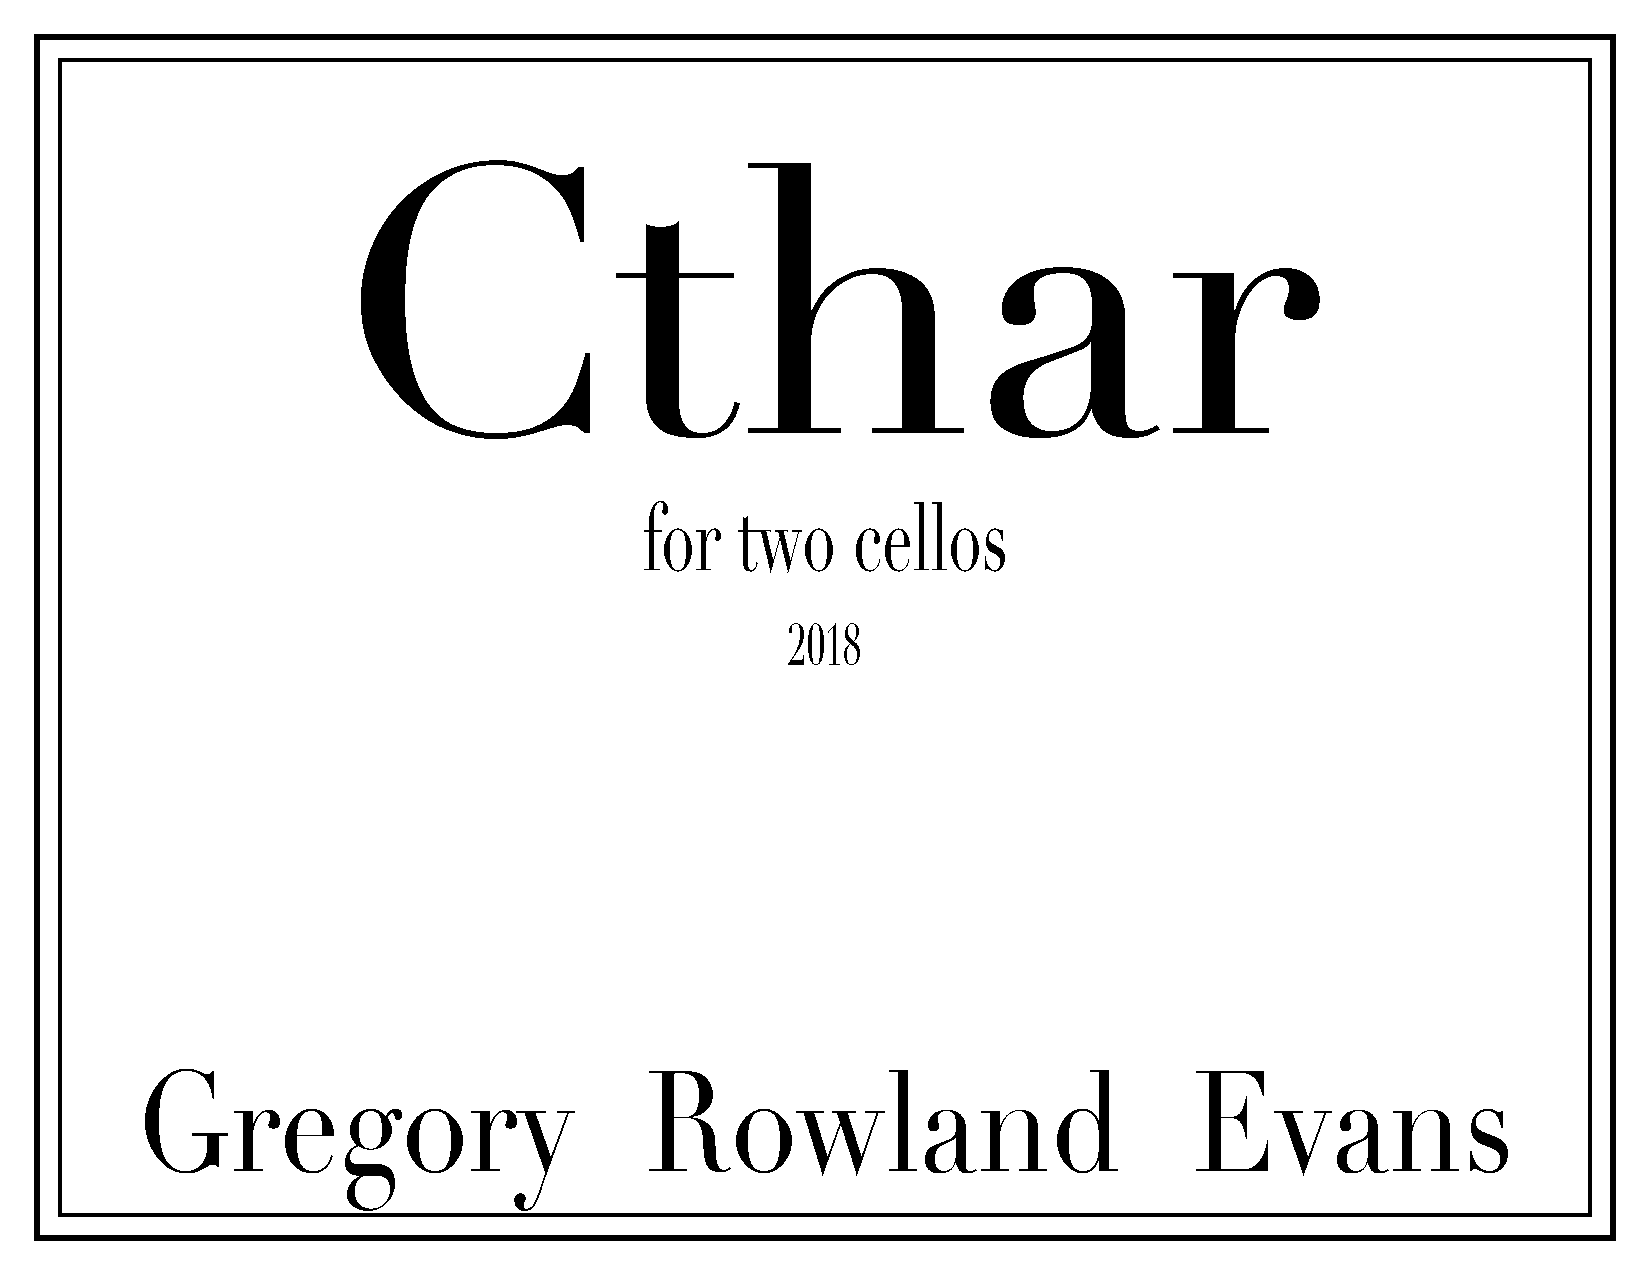
\includepdf[pages=-, pagecommand={}, width=7in,
  height=9.5in, keepaspectratio]{figures/Score/cthar_Score.pdf}

\subsection{Tianshu (for 12 players) Score}

\includepdf[pages=-, pagecommand={},  width=7in,
  height=9.5in, keepaspectratio]{figures/Score/Tianshu_Score.pdf}

\subsection{Four Ages of Sand (for flute, alto saxophone, and violoncello) Score}
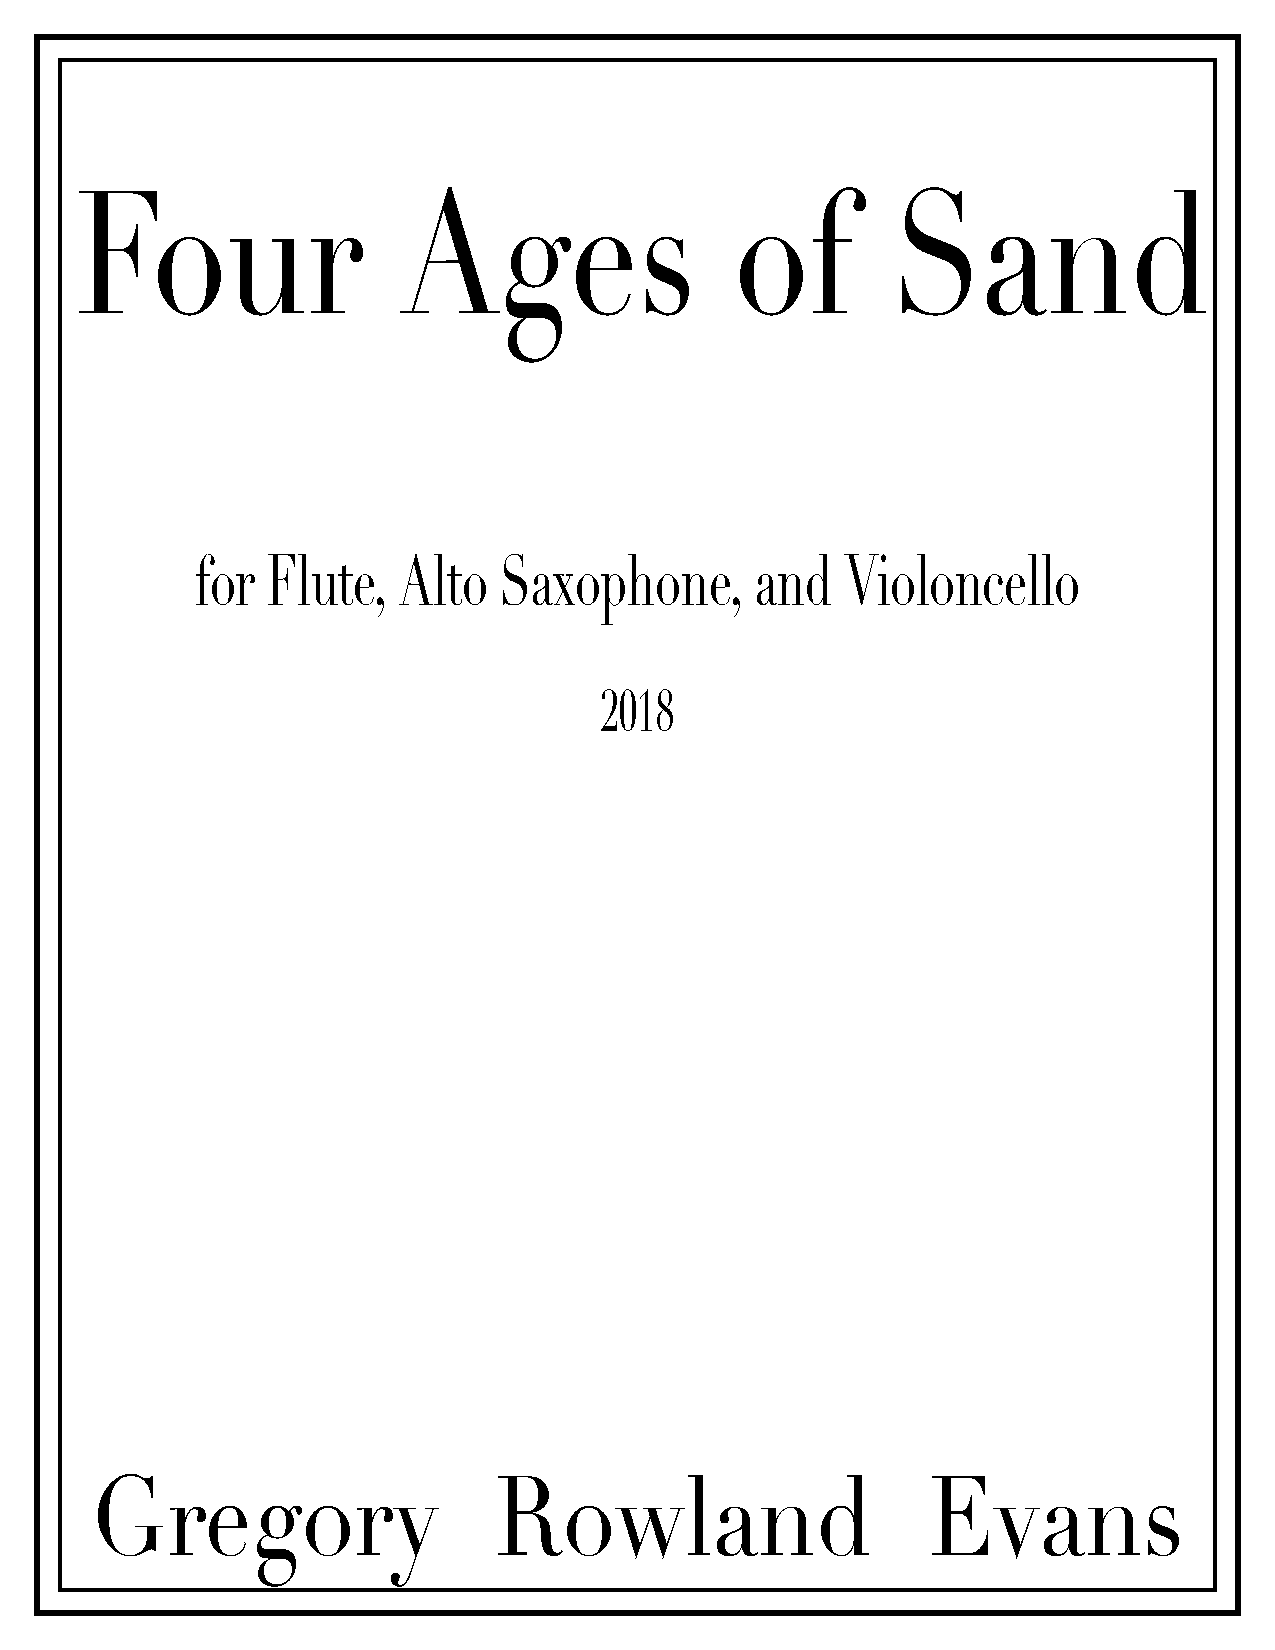
\includepdf[pages=-, pagecommand={},  width=7in,
  height=9.5in, keepaspectratio]{figures/Score/Sand_Score.pdf}

\singlespacing

% the back matter
\clearpage
\bibliography{references}
\addcontentsline{toc}{chapter}{References}
\bibliographystyle{plainnat}
\chapter*{Colophon}

\begin{figure}[h]
    \centering
  
\includegraphics[width=0.50\linewidth]{figures/walk1000.jpg}
  \caption{A 2-dimensional random walk of 1000 iterations by Paul Bourke.}
  \label{fig:1000-iteration random walk}
\end{figure}

\begin{center}
\parbox{200pt}{\raggedright\lettrine[lines=3,slope=-2pt,nindent=-4pt]{\textcolor{Crimson}{T}}{his thesis was typeset} using \LaTeX, originally developed by Leslie Lamport and based on Donald Knuth's \TeX. The body text is set in 12 point Arno Pro, designed by Robert Slimbach in the style of book types from the Aldine Press in Venice, and issued by Adobe in 2007. A template, which can be used to format a PhD thesis with this look and feel, has been released under the permissive \textsc{mit} (\textsc{x}11) license, and can be found online at \href{https://github.com/suchow/}{github.com/suchow/} or from the author at \href{mailto:suchow@fas.harvard.edu}{suchow@post.harvard.edu}.
}
\end{center}

\end{document}
